% Options for packages loaded elsewhere
\PassOptionsToPackage{unicode}{hyperref}
\PassOptionsToPackage{hyphens}{url}
%
\documentclass[
]{article}
\usepackage{amsmath,amssymb}
\usepackage{iftex}
\ifPDFTeX
  \usepackage[T1]{fontenc}
  \usepackage[utf8]{inputenc}
  \usepackage{textcomp} % provide euro and other symbols
\else % if luatex or xetex
  \usepackage{unicode-math} % this also loads fontspec
  \defaultfontfeatures{Scale=MatchLowercase}
  \defaultfontfeatures[\rmfamily]{Ligatures=TeX,Scale=1}
\fi
\usepackage{lmodern}
\ifPDFTeX\else
  % xetex/luatex font selection
\fi
% Use upquote if available, for straight quotes in verbatim environments
\IfFileExists{upquote.sty}{\usepackage{upquote}}{}
\IfFileExists{microtype.sty}{% use microtype if available
  \usepackage[]{microtype}
  \UseMicrotypeSet[protrusion]{basicmath} % disable protrusion for tt fonts
}{}
\makeatletter
\@ifundefined{KOMAClassName}{% if non-KOMA class
  \IfFileExists{parskip.sty}{%
    \usepackage{parskip}
  }{% else
    \setlength{\parindent}{0pt}
    \setlength{\parskip}{6pt plus 2pt minus 1pt}}
}{% if KOMA class
  \KOMAoptions{parskip=half}}
\makeatother
\usepackage{xcolor}
\usepackage[margin=1in]{geometry}
\usepackage{color}
\usepackage{fancyvrb}
\newcommand{\VerbBar}{|}
\newcommand{\VERB}{\Verb[commandchars=\\\{\}]}
\DefineVerbatimEnvironment{Highlighting}{Verbatim}{commandchars=\\\{\}}
% Add ',fontsize=\small' for more characters per line
\usepackage{framed}
\definecolor{shadecolor}{RGB}{248,248,248}
\newenvironment{Shaded}{\begin{snugshade}}{\end{snugshade}}
\newcommand{\AlertTok}[1]{\textcolor[rgb]{0.94,0.16,0.16}{#1}}
\newcommand{\AnnotationTok}[1]{\textcolor[rgb]{0.56,0.35,0.01}{\textbf{\textit{#1}}}}
\newcommand{\AttributeTok}[1]{\textcolor[rgb]{0.13,0.29,0.53}{#1}}
\newcommand{\BaseNTok}[1]{\textcolor[rgb]{0.00,0.00,0.81}{#1}}
\newcommand{\BuiltInTok}[1]{#1}
\newcommand{\CharTok}[1]{\textcolor[rgb]{0.31,0.60,0.02}{#1}}
\newcommand{\CommentTok}[1]{\textcolor[rgb]{0.56,0.35,0.01}{\textit{#1}}}
\newcommand{\CommentVarTok}[1]{\textcolor[rgb]{0.56,0.35,0.01}{\textbf{\textit{#1}}}}
\newcommand{\ConstantTok}[1]{\textcolor[rgb]{0.56,0.35,0.01}{#1}}
\newcommand{\ControlFlowTok}[1]{\textcolor[rgb]{0.13,0.29,0.53}{\textbf{#1}}}
\newcommand{\DataTypeTok}[1]{\textcolor[rgb]{0.13,0.29,0.53}{#1}}
\newcommand{\DecValTok}[1]{\textcolor[rgb]{0.00,0.00,0.81}{#1}}
\newcommand{\DocumentationTok}[1]{\textcolor[rgb]{0.56,0.35,0.01}{\textbf{\textit{#1}}}}
\newcommand{\ErrorTok}[1]{\textcolor[rgb]{0.64,0.00,0.00}{\textbf{#1}}}
\newcommand{\ExtensionTok}[1]{#1}
\newcommand{\FloatTok}[1]{\textcolor[rgb]{0.00,0.00,0.81}{#1}}
\newcommand{\FunctionTok}[1]{\textcolor[rgb]{0.13,0.29,0.53}{\textbf{#1}}}
\newcommand{\ImportTok}[1]{#1}
\newcommand{\InformationTok}[1]{\textcolor[rgb]{0.56,0.35,0.01}{\textbf{\textit{#1}}}}
\newcommand{\KeywordTok}[1]{\textcolor[rgb]{0.13,0.29,0.53}{\textbf{#1}}}
\newcommand{\NormalTok}[1]{#1}
\newcommand{\OperatorTok}[1]{\textcolor[rgb]{0.81,0.36,0.00}{\textbf{#1}}}
\newcommand{\OtherTok}[1]{\textcolor[rgb]{0.56,0.35,0.01}{#1}}
\newcommand{\PreprocessorTok}[1]{\textcolor[rgb]{0.56,0.35,0.01}{\textit{#1}}}
\newcommand{\RegionMarkerTok}[1]{#1}
\newcommand{\SpecialCharTok}[1]{\textcolor[rgb]{0.81,0.36,0.00}{\textbf{#1}}}
\newcommand{\SpecialStringTok}[1]{\textcolor[rgb]{0.31,0.60,0.02}{#1}}
\newcommand{\StringTok}[1]{\textcolor[rgb]{0.31,0.60,0.02}{#1}}
\newcommand{\VariableTok}[1]{\textcolor[rgb]{0.00,0.00,0.00}{#1}}
\newcommand{\VerbatimStringTok}[1]{\textcolor[rgb]{0.31,0.60,0.02}{#1}}
\newcommand{\WarningTok}[1]{\textcolor[rgb]{0.56,0.35,0.01}{\textbf{\textit{#1}}}}
\usepackage{graphicx}
\makeatletter
\def\maxwidth{\ifdim\Gin@nat@width>\linewidth\linewidth\else\Gin@nat@width\fi}
\def\maxheight{\ifdim\Gin@nat@height>\textheight\textheight\else\Gin@nat@height\fi}
\makeatother
% Scale images if necessary, so that they will not overflow the page
% margins by default, and it is still possible to overwrite the defaults
% using explicit options in \includegraphics[width, height, ...]{}
\setkeys{Gin}{width=\maxwidth,height=\maxheight,keepaspectratio}
% Set default figure placement to htbp
\makeatletter
\def\fps@figure{htbp}
\makeatother
\usepackage{soul}
\setlength{\emergencystretch}{3em} % prevent overfull lines
\providecommand{\tightlist}{%
  \setlength{\itemsep}{0pt}\setlength{\parskip}{0pt}}
\setcounter{secnumdepth}{-\maxdimen} % remove section numbering
\ifLuaTeX
  \usepackage{selnolig}  % disable illegal ligatures
\fi
\IfFileExists{bookmark.sty}{\usepackage{bookmark}}{\usepackage{hyperref}}
\IfFileExists{xurl.sty}{\usepackage{xurl}}{} % add URL line breaks if available
\urlstyle{same}
\hypersetup{
  pdftitle={Practica final Aprendizaje Computacional},
  pdfauthor={Manuel Francisco Hidalgo Ros Javier García Masegosa Javier Prior Gomez},
  hidelinks,
  pdfcreator={LaTeX via pandoc}}

\title{Practica final Aprendizaje Computacional}
\author{Manuel Francisco Hidalgo Ros Javier García Masegosa Javier Prior
Gomez}
\date{}

\begin{document}
\maketitle

{
\setcounter{tocdepth}{2}
\tableofcontents
}
\begin{Shaded}
\begin{Highlighting}[]
\CommentTok{\#setwd("/home/manu/FIUM/TERCERO/PrimerCuatri/AC/Proyecto/PracticasAC")}

\ControlFlowTok{if}\NormalTok{(}\SpecialCharTok{!}\FunctionTok{require}\NormalTok{(}\StringTok{"caret"}\NormalTok{)) \{}
  \FunctionTok{install.packages}\NormalTok{(}\StringTok{"caret"}\NormalTok{, }\AttributeTok{dependencies =} \FunctionTok{c}\NormalTok{(}\StringTok{"Depends"}\NormalTok{, }\StringTok{"Suggests"}\NormalTok{))}
  \FunctionTok{require}\NormalTok{(caret)}
\NormalTok{\}}
\end{Highlighting}
\end{Shaded}

\begin{verbatim}
## Loading required package: caret
\end{verbatim}

\begin{verbatim}
## Loading required package: ggplot2
\end{verbatim}

\begin{verbatim}
## Loading required package: lattice
\end{verbatim}

\begin{Shaded}
\begin{Highlighting}[]
\CommentTok{\# Descargamos la base de datos}
\NormalTok{url }\OtherTok{\textless{}{-}} \StringTok{"https://archive.ics.uci.edu/static/public/27/credit+approval.zip"}
\FunctionTok{download.file}\NormalTok{(url, }\AttributeTok{destfile =} \StringTok{"credit\_approval.zip"}\NormalTok{)}


\CommentTok{\# Descomprimimos la base de datos}
\FunctionTok{unzip}\NormalTok{(}\StringTok{"credit\_approval.zip"}\NormalTok{)}


\CommentTok{\# Cargamos la base de datos, na.string = "?" quitamos los datos con ese valor y lo sustituye por NA}
\NormalTok{credit }\OtherTok{\textless{}{-}} \FunctionTok{read.table}\NormalTok{(}\StringTok{"crx.data"}\NormalTok{, }\AttributeTok{header =} \ConstantTok{FALSE}\NormalTok{, }\AttributeTok{sep =} \StringTok{","}\NormalTok{, }\AttributeTok{na.strings =} \StringTok{"?"}\NormalTok{)}


\CommentTok{\# Cargamos en credit.trainIdx la base de datos descargada del UCI}
\NormalTok{credit.trainIdx}\OtherTok{\textless{}{-}}\FunctionTok{readRDS}\NormalTok{(}\StringTok{"credit.trainIdx.rds"}\NormalTok{)}
\NormalTok{credit.Datos.Train}\OtherTok{\textless{}{-}}\NormalTok{credit[credit.trainIdx,]}
\NormalTok{credit.Datos.Test}\OtherTok{\textless{}{-}}\NormalTok{credit[}\SpecialCharTok{{-}}\NormalTok{credit.trainIdx,]}

\CommentTok{\# Crear un indicador para cada conjunto}
\NormalTok{credit.Datos.Train}\SpecialCharTok{$}\NormalTok{Origen }\OtherTok{\textless{}{-}} \StringTok{"train"}
\NormalTok{credit.Datos.Test}\SpecialCharTok{$}\NormalTok{Origen }\OtherTok{\textless{}{-}} \StringTok{"test"}

\CommentTok{\# Combinar los conjuntos}
\NormalTok{combined\_credit }\OtherTok{\textless{}{-}} \FunctionTok{rbind}\NormalTok{(credit.Datos.Train, credit.Datos.Test)}

\CommentTok{\# Librerias usadas durante la practica}
\FunctionTok{library}\NormalTok{(caret)}
\FunctionTok{library}\NormalTok{(randomForest)}
\end{Highlighting}
\end{Shaded}

\begin{verbatim}
## randomForest 4.7-1.2
\end{verbatim}

\begin{verbatim}
## Type rfNews() to see new features/changes/bug fixes.
\end{verbatim}

\begin{verbatim}
## 
## Attaching package: 'randomForest'
\end{verbatim}

\begin{verbatim}
## The following object is masked from 'package:ggplot2':
## 
##     margin
\end{verbatim}

\begin{Shaded}
\begin{Highlighting}[]
\FunctionTok{library}\NormalTok{(nnet)}
\FunctionTok{library}\NormalTok{(pROC)}
\end{Highlighting}
\end{Shaded}

\begin{verbatim}
## Type 'citation("pROC")' for a citation.
\end{verbatim}

\begin{verbatim}
## 
## Attaching package: 'pROC'
\end{verbatim}

\begin{verbatim}
## The following objects are masked from 'package:stats':
## 
##     cov, smooth, var
\end{verbatim}

\begin{Shaded}
\begin{Highlighting}[]
\FunctionTok{library}\NormalTok{(reshape2)}
\FunctionTok{library}\NormalTok{(ggplot2)}
\end{Highlighting}
\end{Shaded}

\hypertarget{introducciuxf3n}{%
\section{Introducción}\label{introducciuxf3n}}

El documento ha cargado automáticamente la base de datos, ahora vamos a
ir haciendo un preprocesado de los datos, primero el siguiente comando
muestra la cantidad de valores NA por columna:

\begin{Shaded}
\begin{Highlighting}[]
\FunctionTok{colSums}\NormalTok{(}\FunctionTok{is.na}\NormalTok{(credit))}
\end{Highlighting}
\end{Shaded}

\begin{verbatim}
##  V1  V2  V3  V4  V5  V6  V7  V8  V9 V10 V11 V12 V13 V14 V15 V16 
##  12  12   0   6   6   9   9   0   0   0   0   0   0  13   0   0
\end{verbatim}

Esto es por si alguna columna tiene demasiados valores NA para
eliminarla

Convertir automáticamente columnas de tipo `chr' a `factor'

\begin{Shaded}
\begin{Highlighting}[]
\NormalTok{credit[}\FunctionTok{sapply}\NormalTok{(credit, is.character)] }\OtherTok{\textless{}{-}} \FunctionTok{lapply}\NormalTok{(credit[}\FunctionTok{sapply}\NormalTok{(credit, is.character)], as.factor)}
\end{Highlighting}
\end{Shaded}

Despues de esto empezamos especulando el significado de cada uno de las
variables. Esto lo vamos a hacer buscando en internet el significado
esperado de cada una, haciendo suposiciones y comprobando que el
análisis de cada una de las variables sea coherente.

\hypertarget{anuxe1lisis-de-variables}{%
\section{Análisis de Variables}\label{anuxe1lisis-de-variables}}

\hypertarget{v1}{%
\subsection{V1}\label{v1}}

Se trata de una variable categórica, con valores en el dominio
\texttt{\{a,\ b\}}. Tiene un significado que podemos intuir de forma
relativamente fácil. De hecho, podemos pensar que ``a'' se trata de
mujeres y ``b'' de hombres. Esto se debe a que la base es de los años
80, y en esa época era más común que los hombres soliciten créditos, y
en el caso de las mujeres, seguramente las que lo solicitaban eran las
que estaban solteras. Se trata de una época con pensamientos cerrados, y
esto es un simple estudio estadístico.

\begin{Shaded}
\begin{Highlighting}[]
\CommentTok{\# Eliminamos niveles no usados}
\NormalTok{credit}\SpecialCharTok{$}\NormalTok{V1 }\OtherTok{\textless{}{-}} \FunctionTok{droplevels}\NormalTok{(credit}\SpecialCharTok{$}\NormalTok{V1)}
\FunctionTok{summary}\NormalTok{(credit}\SpecialCharTok{$}\NormalTok{V1)}
\end{Highlighting}
\end{Shaded}

\begin{verbatim}
##    a    b NA's 
##  210  468   12
\end{verbatim}

Como podemos comprobar nuestra suposición puede ser cierta.

\hypertarget{v2}{%
\subsection{V2}\label{v2}}

Esta columna puede ser la edad del cliente. Es continuo ya que los días
los puede estar teniendo en cuenta de alguna forma. Sin embargo, en
Estados Unidos los menores no pueden solicitar un crédito y hay algunos
valores menores de 18. Vamos a calcular cuantos:

\begin{Shaded}
\begin{Highlighting}[]
\NormalTok{num\_menores\_18 }\OtherTok{\textless{}{-}} \FunctionTok{sum}\NormalTok{(credit}\SpecialCharTok{$}\NormalTok{V2 }\SpecialCharTok{\textless{}} \DecValTok{18}\NormalTok{, }\AttributeTok{na.rm =} \ConstantTok{TRUE}\NormalTok{)}
\NormalTok{total\_valores }\OtherTok{\textless{}{-}} \FunctionTok{sum}\NormalTok{(}\SpecialCharTok{!}\FunctionTok{is.na}\NormalTok{(credit}\SpecialCharTok{$}\NormalTok{V2))}
\NormalTok{porcentaje\_menores\_18 }\OtherTok{\textless{}{-}}\NormalTok{ (num\_menores\_18 }\SpecialCharTok{/}\NormalTok{ total\_valores) }\SpecialCharTok{*} \DecValTok{100}
\NormalTok{porcentaje\_menores\_18}
\end{Highlighting}
\end{Shaded}

\begin{verbatim}
## [1] 5.162242
\end{verbatim}

Comprobamos que aproximadamente el 5\% de los clientes son menores de
edad, al no ser una cifra muy significativa, podemos asumir que son
valores fuera de rango, y que efectivamente podríamos estar ante la
variable de edad. En siguientes apartados veremos qué hacer con estos
valores.

Decidimos que es interesante analizar V2 ya que su media y mediana son
parecidas, lo cual sugiere que la distribución puede ser simétrica
(cercana a normal).

Generamos un histograma base con la función hist() de R para la variable
V2 con probability = TRUE para mostrar la densidad en vez de las
frecuencias absolutas. Además añadimos una línea de densidad para
observar la forma de la distribución de V2, usando la función lines() y
especificando el color ``blue'' para la curva.

\begin{Shaded}
\begin{Highlighting}[]
\FunctionTok{hist}\NormalTok{(credit}\SpecialCharTok{$}\NormalTok{V2, }\AttributeTok{probability =} \ConstantTok{TRUE}\NormalTok{, }\AttributeTok{main =} \StringTok{"Histograma de V2 con Curva de Densidad"}\NormalTok{)}
\FunctionTok{lines}\NormalTok{(}\FunctionTok{density}\NormalTok{(credit}\SpecialCharTok{$}\NormalTok{V2, }\AttributeTok{na.rm =} \ConstantTok{TRUE}\NormalTok{), }\AttributeTok{col =} \StringTok{"blue"}\NormalTok{)}
\end{Highlighting}
\end{Shaded}

\includegraphics{PreprocesadoDeDatos_files/figure-latex/unnamed-chunk-5-1.pdf}

Creamos un histograma con ggplot2 para la variable V2 del dataframe
`credit', estableciendo aesthetic mapping (aes) para usar V2 en el eje x
y ademas y añadimos un histograma con color de contorno naranja y
relleno naranja claro (alpha = 0.2) y definimos intervalos de 5 unidades
usando el argumento breaks.

\begin{Shaded}
\begin{Highlighting}[]
\NormalTok{myHist }\OtherTok{\textless{}{-}} \FunctionTok{ggplot}\NormalTok{(}\AttributeTok{data =}\NormalTok{ credit, }\FunctionTok{aes}\NormalTok{(}\AttributeTok{x =}\NormalTok{ V2)) }\SpecialCharTok{+}
  \FunctionTok{geom\_histogram}\NormalTok{(}\AttributeTok{col =} \StringTok{"orange"}\NormalTok{, }\AttributeTok{fill =} \StringTok{"orange"}\NormalTok{, }\AttributeTok{alpha =} \FloatTok{0.2}\NormalTok{, }\AttributeTok{breaks =} \FunctionTok{seq}\NormalTok{(}\DecValTok{0}\NormalTok{, }\DecValTok{80}\NormalTok{, }\AttributeTok{by =} \DecValTok{5}\NormalTok{)) }\SpecialCharTok{+}
  \FunctionTok{geom\_density}\NormalTok{(}\AttributeTok{col =} \StringTok{"blue"}\NormalTok{, }\AttributeTok{lwd =} \DecValTok{1}\NormalTok{) }\SpecialCharTok{+}
  \FunctionTok{labs}\NormalTok{(}\AttributeTok{title =} \StringTok{"Histograma para la variable V2 con línea de densidad"}\NormalTok{, }\AttributeTok{x =} \StringTok{"V2"}\NormalTok{, }\AttributeTok{y =} \StringTok{"Frecuencia"}\NormalTok{)}

\CommentTok{\# Mostrar el gráfico}
\NormalTok{myHist}
\end{Highlighting}
\end{Shaded}

\begin{verbatim}
## Warning: Removed 12 rows containing non-finite outside the scale range
## (`stat_bin()`).
\end{verbatim}

\begin{verbatim}
## Warning: Removed 12 rows containing non-finite outside the scale range
## (`stat_density()`).
\end{verbatim}

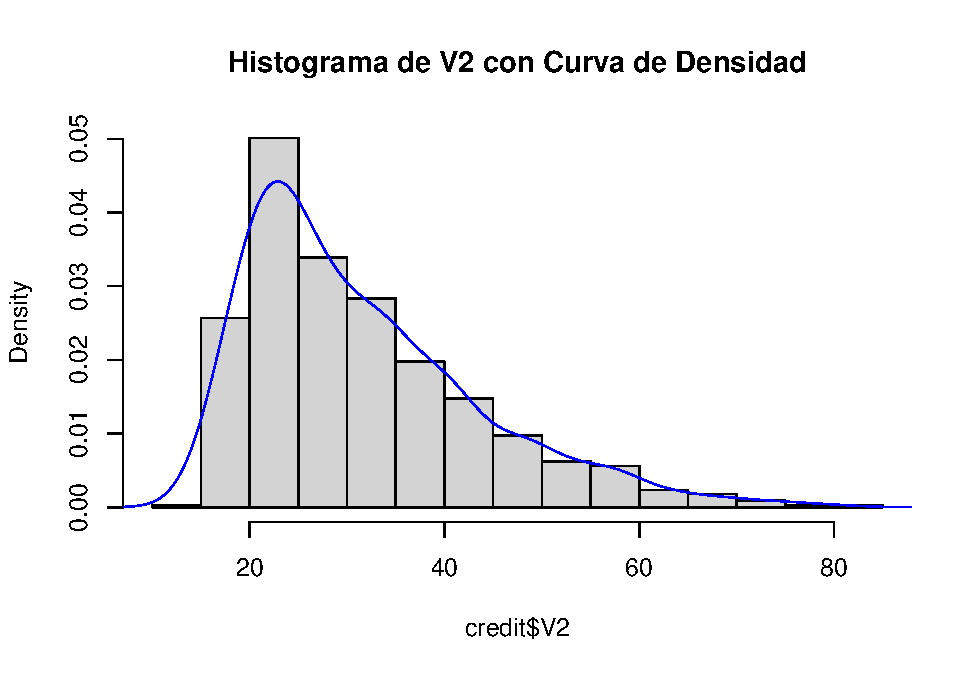
\includegraphics{PreprocesadoDeDatos_files/figure-latex/unnamed-chunk-6-1.pdf}

Añadimos una línea vertical en el histograma de ggplot para marcar la
media de V2 usando geom\_vline() y especificando la posición con
xintercept = mean() y hacemos lo mismo para marcar la mediana.

\begin{Shaded}
\begin{Highlighting}[]
\NormalTok{myHist }\OtherTok{=}\NormalTok{ myHist }\SpecialCharTok{+} \FunctionTok{geom\_vline}\NormalTok{(}\AttributeTok{xintercept =} \FunctionTok{mean}\NormalTok{(credit}\SpecialCharTok{$}\NormalTok{V2, }\AttributeTok{na.rm =} \ConstantTok{TRUE}\NormalTok{), }\AttributeTok{col =} \StringTok{"blue"}\NormalTok{)}
\NormalTok{myHist }\OtherTok{=}\NormalTok{ myHist }\SpecialCharTok{+} \FunctionTok{geom\_vline}\NormalTok{(}\AttributeTok{xintercept =} \FunctionTok{median}\NormalTok{(credit}\SpecialCharTok{$}\NormalTok{V2, }\AttributeTok{na.rm =} \ConstantTok{TRUE}\NormalTok{), }\AttributeTok{col =} \StringTok{"red"}\NormalTok{)}
\end{Highlighting}
\end{Shaded}

Mostramos el gráfico final en ggplot2 con el histograma de V2, junto con
las líneas de media (azul) y mediana (roja).

\begin{Shaded}
\begin{Highlighting}[]
\NormalTok{myHist}
\end{Highlighting}
\end{Shaded}

\begin{verbatim}
## Warning: Removed 12 rows containing non-finite outside the scale range
## (`stat_bin()`).
\end{verbatim}

\begin{verbatim}
## Warning: Removed 12 rows containing non-finite outside the scale range
## (`stat_density()`).
\end{verbatim}

\includegraphics{PreprocesadoDeDatos_files/figure-latex/unnamed-chunk-8-1.pdf}

Como vemos, V2 no sigue exactamente una distribución normal, ya que la
media y la mediana no son idénticas, lo que indica una posible asimetría
en los datos.

Para confirmar formalmente la falta de normalidad, realizaremos un
gráfico Q-Q (Quantile-Quantile), que nos permite comparar la
distribución de V2 con la distribución teórica normal.

\begin{Shaded}
\begin{Highlighting}[]
\CommentTok{\# Creamos el gráfico Q{-}Q para V2 utilizando ggplot2.}
\NormalTok{p1 }\OtherTok{=} \FunctionTok{ggplot}\NormalTok{(}\AttributeTok{data =}\NormalTok{ credit, }\FunctionTok{aes}\NormalTok{(}\AttributeTok{sample =}\NormalTok{ V2)) }\SpecialCharTok{+}
  \CommentTok{\# Añadimos un título al gráfico Q{-}Q.}
  \FunctionTok{ggtitle}\NormalTok{(}\StringTok{"QQ plot para V2"}\NormalTok{) }\SpecialCharTok{+}
  \CommentTok{\# Añadimos los puntos del gráfico Q{-}Q, que compara los cuantiles de la muestra de V2 }
  \CommentTok{\# con los cuantiles teóricos de una distribución normal.}
  \FunctionTok{geom\_qq}\NormalTok{() }\SpecialCharTok{+} 
  \CommentTok{\# Añadimos la línea Q{-}Q teórica (stat\_qq\_line), que muestra cómo se deberían }
  \CommentTok{\# alinear los puntos si la distribución de V2 fuera normal.}
  \FunctionTok{stat\_qq\_line}\NormalTok{() }\SpecialCharTok{+} 
  \CommentTok{\# Etiquetas para los ejes: \textquotesingle{}Distribución teórica\textquotesingle{} en el eje x y \textquotesingle{}Distribución muestral\textquotesingle{} en el eje y.}
  \FunctionTok{xlab}\NormalTok{(}\StringTok{"Distribución teórica"}\NormalTok{) }\SpecialCharTok{+} 
  \FunctionTok{ylab}\NormalTok{(}\StringTok{"Distribución muestral"}\NormalTok{)}
\end{Highlighting}
\end{Shaded}

Mostramos el gráfico Q-Q, que permite ver si los puntos se alinean (lo
que indicaría normalidad) o si se desvían de la línea (indicando falta
de normalidad en la distribución de V2).

\begin{Shaded}
\begin{Highlighting}[]
\NormalTok{p1}
\end{Highlighting}
\end{Shaded}

\begin{verbatim}
## Warning: Removed 12 rows containing non-finite outside the scale range
## (`stat_qq()`).
\end{verbatim}

\begin{verbatim}
## Warning: Removed 12 rows containing non-finite outside the scale range
## (`stat_qq_line()`).
\end{verbatim}

\includegraphics{PreprocesadoDeDatos_files/figure-latex/unnamed-chunk-10-1.pdf}

Como vemos hay una desviación de la diagonal. Por tanto, podemos
concluir que no se trata de una distribución normal.

\hypertarget{v3}{%
\subsection{V3}\label{v3}}

Nuestra especulación en cuanto a esta columna es que se trata de la
cantidad de deuda que tienen los clientes. Sin embargo, no tiene sentido
que el que más debe, el total sea 28\$:

\begin{Shaded}
\begin{Highlighting}[]
\FunctionTok{summary}\NormalTok{(credit}\SpecialCharTok{$}\NormalTok{V3)}
\end{Highlighting}
\end{Shaded}

\begin{verbatim}
##    Min. 1st Qu.  Median    Mean 3rd Qu.    Max. 
##   0.000   1.000   2.750   4.759   7.207  28.000
\end{verbatim}

Por ello, pensamos que pueda estar dividida por \(10^{3}\) o similar. De
igual manera no nos importa la proporción que lleve.

\hypertarget{v4}{%
\subsection{V4}\label{v4}}

En esta columna podríamos estar ante el estado civil de cada uno de los
clientes. Siendo cada uno de los valores \{l=desconocido, u=casados,
y=solteros, t=otros\}. Si calculamos el porcentaje de clientes casados:

\begin{Shaded}
\begin{Highlighting}[]
\NormalTok{num\_mayores\_18 }\OtherTok{\textless{}{-}} \FunctionTok{sum}\NormalTok{(credit}\SpecialCharTok{$}\NormalTok{V2 }\SpecialCharTok{\textgreater{}} \DecValTok{18}\NormalTok{, }\AttributeTok{na.rm =} \ConstantTok{TRUE}\NormalTok{)}
\NormalTok{num\_casados }\OtherTok{\textless{}{-}} \FunctionTok{sum}\NormalTok{(credit}\SpecialCharTok{$}\NormalTok{V4 }\SpecialCharTok{==} \StringTok{"u"}\NormalTok{, }\AttributeTok{na.rm =} \ConstantTok{TRUE}\NormalTok{)}
\NormalTok{porcent\_casados }\OtherTok{\textless{}{-}}\NormalTok{ (num\_casados}\SpecialCharTok{/}\NormalTok{num\_mayores\_18) }\SpecialCharTok{*} \DecValTok{100}
\NormalTok{porcent\_casados}
\end{Highlighting}
\end{Shaded}

\begin{verbatim}
## [1] 80.84112
\end{verbatim}

Si buscamos en internet en torno al 70\% de la población adulta en
Estados Unidos estaba casada. Como podemos ver se aproxima mucho a
nuestro resultado. Esa pequeña diferencia puede deberse a que muchos
matrimonios al casarse, compran una casa, y piden un préstamo para ello.

Observamos en V4 que hay un elemento que no aparece y es necesario
añadir.

\begin{Shaded}
\begin{Highlighting}[]
\CommentTok{\# Eliminamos niveles no usados}
\CommentTok{\#credit$V4 \textless{}{-} droplevels(credit$V4)}

\CommentTok{\# Ahora vamos a añadir un elemento que no aparece y luego lo hacemos factor}
\CommentTok{\#levels(credit$V4)\textless{}{-}c(levels(credit$V4),"t")}
\FunctionTok{str}\NormalTok{(credit}\SpecialCharTok{$}\NormalTok{V4)}
\end{Highlighting}
\end{Shaded}

\begin{verbatim}
##  Factor w/ 3 levels "l","u","y": 2 2 2 2 2 2 2 2 3 3 ...
\end{verbatim}

\hypertarget{v6}{%
\subsection{V6}\label{v6}}

Analizamos la variable categórica V6 para obtener una visión general de
su distribución y composición. Mostramos un resumen estadístico de V6,
que nos indica la frecuencia de cada categoría en esta variable.

\begin{Shaded}
\begin{Highlighting}[]
\FunctionTok{summary}\NormalTok{(credit}\SpecialCharTok{$}\NormalTok{V6)}
\end{Highlighting}
\end{Shaded}

\begin{verbatim}
##   aa    c   cc    d    e   ff    i    j    k    m    q    r    w    x NA's 
##   54  137   41   30   25   53   59   10   51   38   78    3   64   38    9
\end{verbatim}

Verificamos la estructura de V6 para confirmar que es una variable
categórica (factor o carácter).

\begin{Shaded}
\begin{Highlighting}[]
\FunctionTok{str}\NormalTok{(credit}\SpecialCharTok{$}\NormalTok{V6)}
\end{Highlighting}
\end{Shaded}

\begin{verbatim}
##  Factor w/ 14 levels "aa","c","cc",..: 13 11 11 13 13 10 12 3 9 13 ...
\end{verbatim}

Calculamos el porcentaje de cada categoría en V6, para ello primero,
obtenemos la frecuencia de cada categoría con table(credit\$V6) y luego,
usamos prop.table() para calcular la proporción relativa de cada
categoría y multiplicamos por 100 para expresarlo en porcentaje.

\begin{Shaded}
\begin{Highlighting}[]
\NormalTok{porcent }\OtherTok{\textless{}{-}} \FunctionTok{prop.table}\NormalTok{(}\FunctionTok{table}\NormalTok{(credit}\SpecialCharTok{$}\NormalTok{V6)) }\SpecialCharTok{*} \DecValTok{100}
\end{Highlighting}
\end{Shaded}

Creamos una tabla que combina tanto el número total de observaciones
(frecuencia) como el porcentaje de cada categoría: cbind() se usa para
unir la frecuencia y el porcentaje en una tabla única.

\begin{Shaded}
\begin{Highlighting}[]
\NormalTok{porcent\_table }\OtherTok{\textless{}{-}} \FunctionTok{cbind}\NormalTok{(}\AttributeTok{total =} \FunctionTok{table}\NormalTok{(credit}\SpecialCharTok{$}\NormalTok{V6), }\AttributeTok{porcentaje =}\NormalTok{ porcent)}
\end{Highlighting}
\end{Shaded}

Mostramos el vector de porcentajes, lo que nos permite visualizar el
porcentaje de cada categoría en V6.

\begin{Shaded}
\begin{Highlighting}[]
\NormalTok{porcent}
\end{Highlighting}
\end{Shaded}

\begin{verbatim}
## 
##         aa          c         cc          d          e         ff          i 
##  7.9295154 20.1174743  6.0205580  4.4052863  3.6710720  7.7826725  8.6637298 
##          j          k          m          q          r          w          x 
##  1.4684288  7.4889868  5.5800294 11.4537445  0.4405286  9.3979442  5.5800294
\end{verbatim}

Ahora que entendemos la distribución de frecuencias y porcentajes de
cada categoría, generamos un gráfico de sectores para visualizar estos
porcentajes de manera gráfica y comparativa.

Creamos el gráfico de sectores (o ``quesos'') usando la función pie(),
pasándole el vector de porcentajes. Establecemos un título con el
argumento main y aplicamos diferentes colores a cada categoría usando
rainbow().

\begin{Shaded}
\begin{Highlighting}[]
\FunctionTok{pie}\NormalTok{(porcent, }\AttributeTok{main =} \StringTok{"Diagrama de Quesos para V6"}\NormalTok{, }\AttributeTok{col =} \FunctionTok{rainbow}\NormalTok{(}\FunctionTok{length}\NormalTok{(porcent)))}
\end{Highlighting}
\end{Shaded}

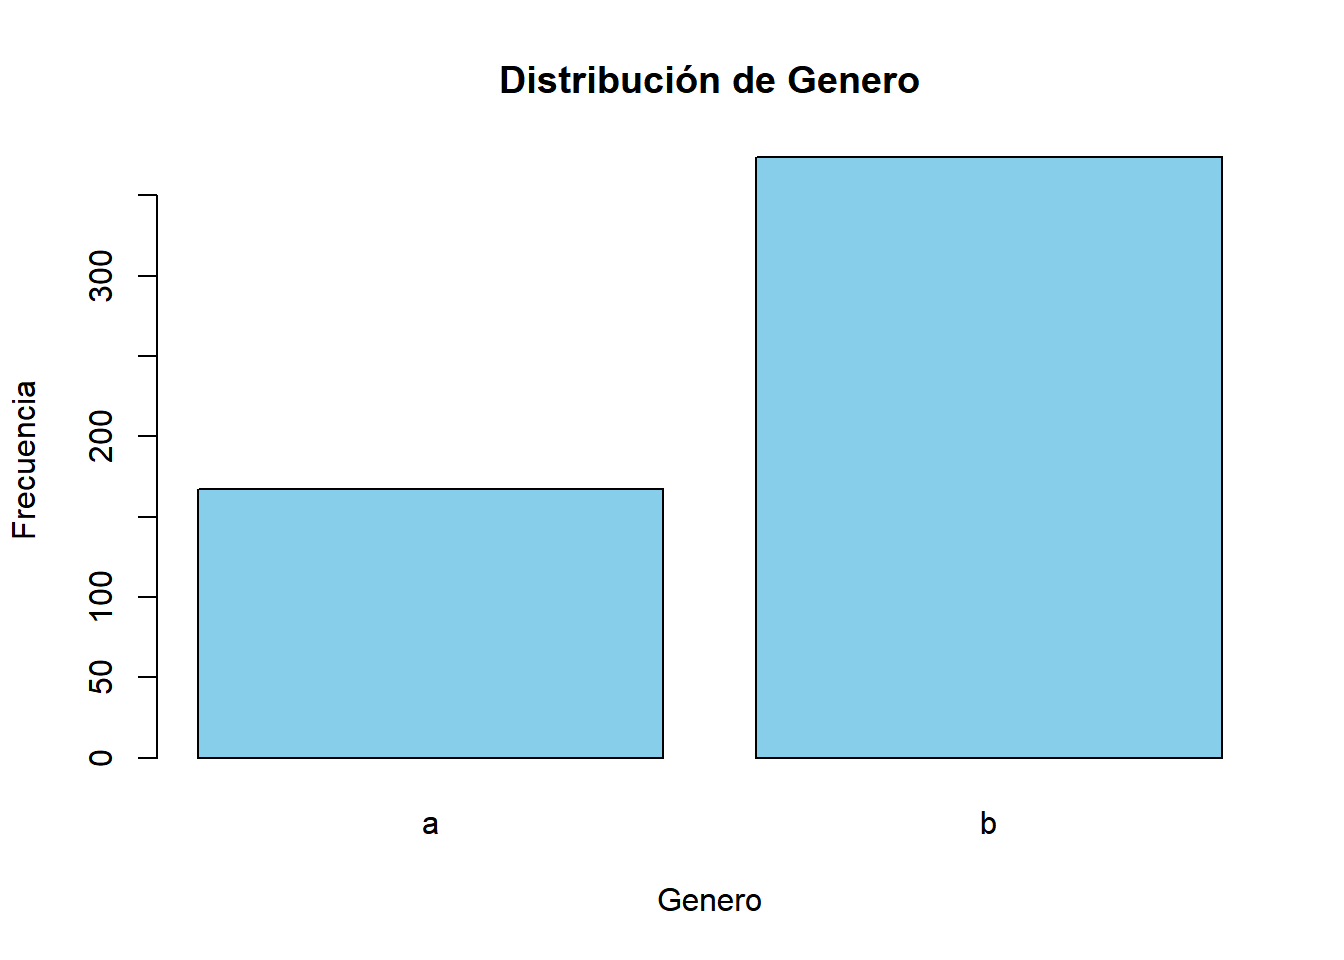
\includegraphics{PreprocesadoDeDatos_files/figure-latex/unnamed-chunk-19-1.pdf}

Mostramos nuevamente el vector de porcentajes para recordar los valores
antes de proceder con el análisis de los valores NA.

\begin{Shaded}
\begin{Highlighting}[]
\NormalTok{porcent}
\end{Highlighting}
\end{Shaded}

\begin{verbatim}
## 
##         aa          c         cc          d          e         ff          i 
##  7.9295154 20.1174743  6.0205580  4.4052863  3.6710720  7.7826725  8.6637298 
##          j          k          m          q          r          w          x 
##  1.4684288  7.4889868  5.5800294 11.4537445  0.4405286  9.3979442  5.5800294
\end{verbatim}

Calculamos la suma del resumen de V6 para confirmar el número total de
observaciones, incluyendo posibles NA.

\begin{Shaded}
\begin{Highlighting}[]
\FunctionTok{sum}\NormalTok{(}\FunctionTok{summary}\NormalTok{(credit}\SpecialCharTok{$}\NormalTok{V6))}
\end{Highlighting}
\end{Shaded}

\begin{verbatim}
## [1] 690
\end{verbatim}

Calculamos el porcentaje de valores NA en la variable V6, asumiendo que
hay 9 valores NA de un total de 690 observaciones.

\begin{Shaded}
\begin{Highlighting}[]
\NormalTok{porcentaje\_na }\OtherTok{\textless{}{-}} \DecValTok{9} \SpecialCharTok{/} \DecValTok{690} \SpecialCharTok{*} \DecValTok{100}
\NormalTok{porcentaje\_na}
\end{Highlighting}
\end{Shaded}

\begin{verbatim}
## [1] 1.304348
\end{verbatim}

Concluimos que, siendo aproximadamente un 1.3\% de valores faltantes
(NA), la eliminación de estas observaciones es razonable, ya que este
porcentaje es bajo y es poco probable que afecte significativamente el
análisis.

\hypertarget{v8}{%
\subsection{V8}\label{v8}}

Esta variable creemos que puede ser los años de empleo. Si nos fijamos
en los valores de las columnas de V8 (años contratado) y las comparamos
por filas con las de V2 (edad) nos podemos dar cuenta que nunca va a
superar la edad. De hecho en muchos casos tiene coherencia la edad con
el número de años contratado. Esto puede ser un claro indicativo que
estamos ante una buena especulación. Aún así vamos a verlo en R:

\begin{Shaded}
\begin{Highlighting}[]
\FunctionTok{summary}\NormalTok{(credit}\SpecialCharTok{$}\NormalTok{V8)}
\end{Highlighting}
\end{Shaded}

\begin{verbatim}
##    Min. 1st Qu.  Median    Mean 3rd Qu.    Max. 
##   0.000   0.165   1.000   2.223   2.625  28.500
\end{verbatim}

Podemos apreciar que el valor máximo no es muy grande. Esto nos puede
despistar un poco, pero basta con informarnos un poco sobre la variable
edad:

\begin{Shaded}
\begin{Highlighting}[]
\FunctionTok{summary}\NormalTok{(credit}\SpecialCharTok{$}\NormalTok{V2)}
\end{Highlighting}
\end{Shaded}

\begin{verbatim}
##    Min. 1st Qu.  Median    Mean 3rd Qu.    Max.    NA's 
##   13.75   22.60   28.46   31.57   38.23   80.25      12
\end{verbatim}

¿Aporta algo este resumen? Por supuesto, de hecho tenemos la razón de
que nuestra variable de años contratados presente datos tan bajos.
Estamos ante un conjunto de clientes jóvenes, y como es lógico no tienen
muchos años como empleados.

\hypertarget{v10}{%
\subsection{V10}\label{v10}}

Esta variable hemos podido intuir junto a alguna investigaciones que
representa si un cliente está actualmente empleado. Esto es muy
interesante de cara al análisis por temas obvios de solvencia. Suponemos
que \{f=empleado, t=no empleado\}. Pero, ¿realmente es consistente la
cifra de empleados? Sí, lo vemos con:

\begin{Shaded}
\begin{Highlighting}[]
\NormalTok{porcentajes\_empleados }\OtherTok{\textless{}{-}} \FunctionTok{prop.table}\NormalTok{(}\FunctionTok{summary}\NormalTok{(credit}\SpecialCharTok{$}\NormalTok{V10))}\SpecialCharTok{*}\DecValTok{100}
\NormalTok{porcentajes\_empleados}
\end{Highlighting}
\end{Shaded}

\begin{verbatim}
##        f        t 
## 57.24638 42.75362
\end{verbatim}

Según hemos podido encontrar en los años ochenta en Estados Unidos había
un 60\% de población activa. Esto es de gran utilidad para hacer una
correlación junto a V16 (aprobada/rechazada).

\hypertarget{v11}{%
\subsection{V11}\label{v11}}

Esta variable es posible que sea ``credit score'', que es es una
expresión numérica que representa la solvencia de un individuo. Según
hemos podido comprobar también ha sido retocada (los valores), ya que
los valores no siguen la notación habitual. Pero sí sabemos que cuanto
mayor es el valor, mayor es la solvencia. En la
Figura\textasciitilde{}\ref{fig:credit_score} podemos encontrar un
gráfico interesante que ilustra este concepto:

\begin{figure}
\centering
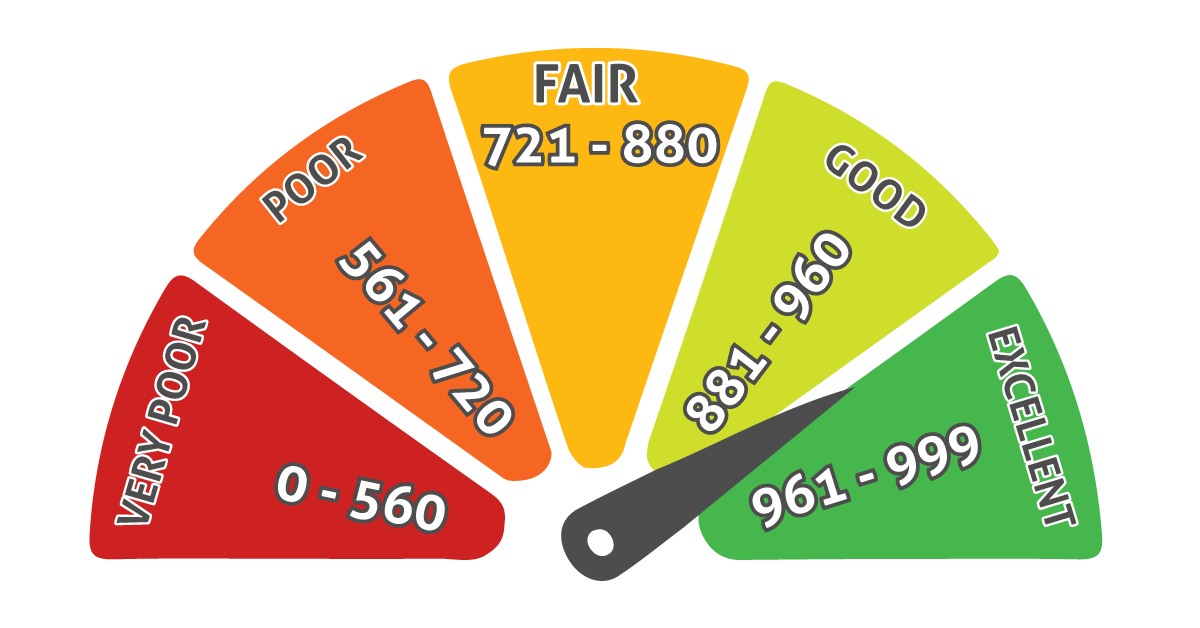
\includegraphics{imagenes/creditScorepx.png}
\caption{Descripción de la imagen}
\end{figure}

Es importante conocer la forma que van a tener nuestros datos de esta
variable:

\begin{Shaded}
\begin{Highlighting}[]
\FunctionTok{hist}\NormalTok{(credit}\SpecialCharTok{$}\NormalTok{V11, }
     \AttributeTok{breaks =} \FunctionTok{seq}\NormalTok{(}\FunctionTok{min}\NormalTok{(credit}\SpecialCharTok{$}\NormalTok{V11, }\AttributeTok{na.rm =} \ConstantTok{TRUE}\NormalTok{), }\FunctionTok{max}\NormalTok{(credit}\SpecialCharTok{$}\NormalTok{V11, }\AttributeTok{na.rm =} \ConstantTok{TRUE}\NormalTok{), }\AttributeTok{by =} \DecValTok{1}\NormalTok{),}
     \AttributeTok{main =} \StringTok{"Histograma de Credit Score V11"}\NormalTok{,}
     \AttributeTok{xlab =} \StringTok{"Valores de V11"}\NormalTok{, }
     \AttributeTok{ylab =} \StringTok{"Frecuencia"}\NormalTok{,}
     \AttributeTok{col =} \StringTok{"lightblue"}\NormalTok{, }
     \AttributeTok{border =} \StringTok{"black"}\NormalTok{)}
\end{Highlighting}
\end{Shaded}

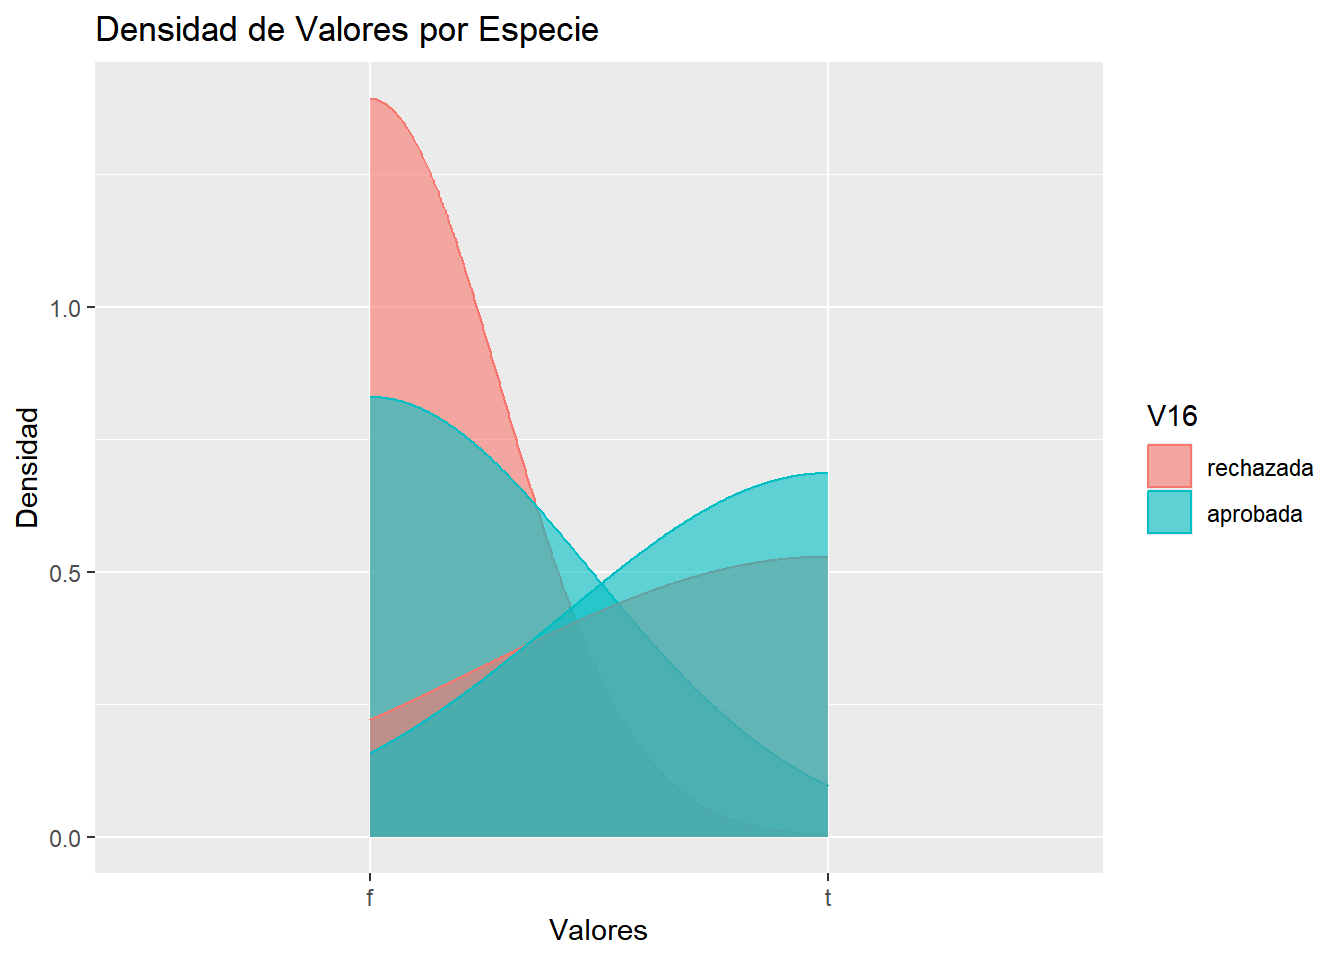
\includegraphics{PreprocesadoDeDatos_files/figure-latex/unnamed-chunk-26-1.pdf}

La mediana indica que hay muchos ceros. Y con el histograma vemos que
esto efectivamente es así:

grafico v11

Lo deberíamos de tener en cuenta a la hora de hacer el análisis
multivariable.

\hypertarget{v13}{%
\subsection{V13}\label{v13}}

Pasamos a analizar la última variable interesante para nuestro análisis.
Esta variable representa composición de la población, clasificando en:
cuidadano, residente permenente o inmigrante. Según consta en los datos,
la distribución es 86\%, 2.6\% y 6.2\%. ¿Se aproximará?

\begin{Shaded}
\begin{Highlighting}[]
\FunctionTok{prop.table}\NormalTok{(}\FunctionTok{summary}\NormalTok{(credit}\SpecialCharTok{$}\NormalTok{V13))}\SpecialCharTok{*}\DecValTok{100}
\end{Highlighting}
\end{Shaded}

\begin{verbatim}
##        g        p        s 
## 90.57971  1.15942  8.26087
\end{verbatim}

Como vemos son muy parecidos. Esto es un indicativo significativo.
Concluimos que \{g=ciudadano, p=residente permanente, s=inmigrante\}.

\hypertarget{razonamiento-para-comparar-v14-y-v16}{%
\subsection{Razonamiento para comparar V14 y
V16}\label{razonamiento-para-comparar-v14-y-v16}}

Una razonamiento útil que podemos hacer es relacionar los códigos
postales con la aprobación de los créditos solicitados. Suponemos que
los códigos postales han sidos modificados de alguna manera para
proteger la privacidad de los datos. Esto lo hacemos porque dependiendo
de la ubicación de los solicitantes, si están en barrios más ricos, o
barrios más humildes, podemos hacer una distinción de gente con más
poder adquisitivo, que por lo general, representarán mayor parte de
solicitudes aprobadas.

\begin{Shaded}
\begin{Highlighting}[]
\FunctionTok{library}\NormalTok{(ggplot2)}
    \FunctionTok{ggplot}\NormalTok{(credit, }\FunctionTok{aes}\NormalTok{(}\AttributeTok{x =}\NormalTok{ V16, }\AttributeTok{y =}\NormalTok{ V14, }\AttributeTok{fill =}\NormalTok{ V16)) }\SpecialCharTok{+} 
        \FunctionTok{geom\_violin}\NormalTok{() }\SpecialCharTok{+}
        \FunctionTok{labs}\NormalTok{(}\AttributeTok{title =} \StringTok{"Distribución de V14 (Edad) por V16 (Decisión de Crédito)"}\NormalTok{,}
            \AttributeTok{x =} \StringTok{"Decisión de Crédito (V16)"}\NormalTok{, }
            \AttributeTok{y =} \StringTok{"Edad (V14)"}\NormalTok{) }\SpecialCharTok{+}
    \FunctionTok{theme\_minimal}\NormalTok{() }\SpecialCharTok{+}
    \FunctionTok{scale\_fill\_manual}\NormalTok{(}\AttributeTok{values =} \FunctionTok{c}\NormalTok{(}\StringTok{"skyblue"}\NormalTok{, }\StringTok{"orange"}\NormalTok{))}
\end{Highlighting}
\end{Shaded}

\begin{verbatim}
## Warning: Removed 13 rows containing non-finite outside the scale range
## (`stat_ydensity()`).
\end{verbatim}

\includegraphics{PreprocesadoDeDatos_files/figure-latex/unnamed-chunk-28-1.pdf}

\hypertarget{v15}{%
\subsection{V15}\label{v15}}

Vamos a analizar la variable V15, que parece tener una distribución con
muchos valores cercanos a 0 pero también valores atípicos elevados, lo
que podría afectar la media.

Realizamos un resumen estadístico de la variable V15 para obtener una
visión general de los valores, incluyendo mínimos, máximos, media y
mediana.

\begin{Shaded}
\begin{Highlighting}[]
\FunctionTok{summary}\NormalTok{(credit}\SpecialCharTok{$}\NormalTok{V15)}
\end{Highlighting}
\end{Shaded}

\begin{verbatim}
##     Min.  1st Qu.   Median     Mean  3rd Qu.     Max. 
##      0.0      0.0      5.0   1017.4    395.5 100000.0
\end{verbatim}

Generamos un histograma básico para observar la distribución de V15.
Usamos probability = TRUE para mostrar el histograma en términos de
densidad. Además añadimos una curva de densidad a la gráfica para
visualizar mejor la forma de la distribución, usando la función
density() con na.rm = TRUE para excluir valores NA.

\begin{Shaded}
\begin{Highlighting}[]
\FunctionTok{hist}\NormalTok{(credit}\SpecialCharTok{$}\NormalTok{V15, }\AttributeTok{probability =} \ConstantTok{TRUE}\NormalTok{,}\AttributeTok{main =} \StringTok{"Histograma de V15 con Curva de Densidad"}\NormalTok{)}
\FunctionTok{lines}\NormalTok{(}\FunctionTok{density}\NormalTok{(credit}\SpecialCharTok{$}\NormalTok{V15, }\AttributeTok{na.rm =} \ConstantTok{TRUE}\NormalTok{), }\AttributeTok{col =} \StringTok{"blue"}\NormalTok{)}
\end{Highlighting}
\end{Shaded}

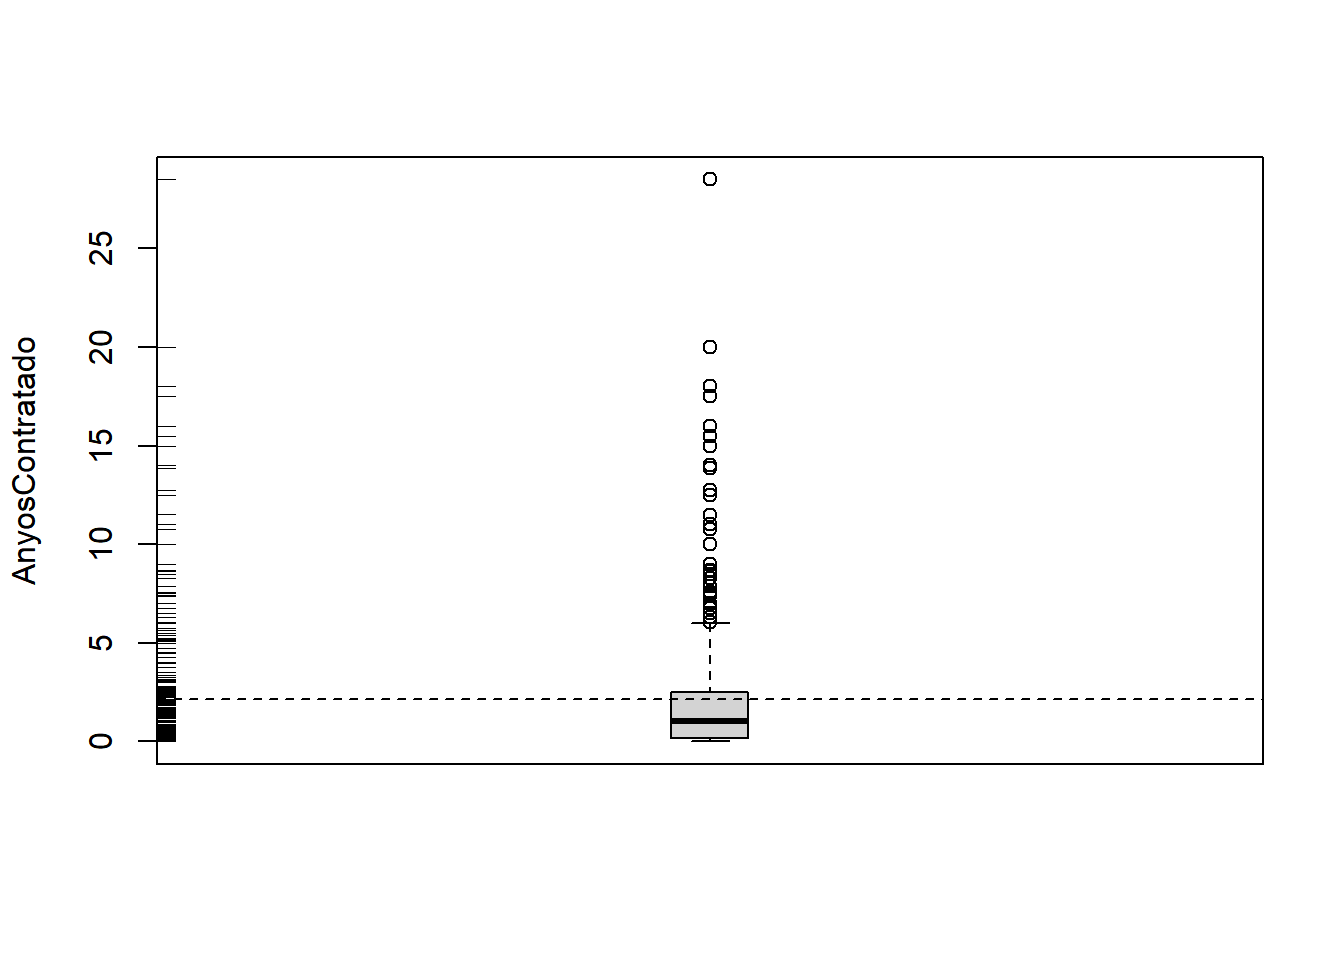
\includegraphics{PreprocesadoDeDatos_files/figure-latex/unnamed-chunk-30-1.pdf}

Observamos que muchos valores altos de V15 hacen difícil ver los valores
menores. Para solucionar esto, usamos ggplot2 para crear un histograma
que enfoque la escala en valores menores, estableciendo los intervalos
hasta 1000 (ajustable según el rango de interés).

Creamos un histograma de V15 con ggplot2, aplicando intervalos de 10 en
el rango de 0 a 1000.

\begin{Shaded}
\begin{Highlighting}[]
\NormalTok{myHist }\OtherTok{=} \FunctionTok{ggplot}\NormalTok{(}\AttributeTok{data =}\NormalTok{ credit, }\FunctionTok{aes}\NormalTok{(credit}\SpecialCharTok{$}\NormalTok{V15)) }\SpecialCharTok{+}
  \FunctionTok{geom\_histogram}\NormalTok{(}\AttributeTok{col =} \StringTok{"orange"}\NormalTok{, }\AttributeTok{fill =} \StringTok{"orange"}\NormalTok{, }\AttributeTok{alpha =} \FloatTok{0.2}\NormalTok{, }\AttributeTok{breaks =} \FunctionTok{seq}\NormalTok{(}\DecValTok{0}\NormalTok{, }\DecValTok{1000}\NormalTok{, }\AttributeTok{by =} \DecValTok{10}\NormalTok{)) }\SpecialCharTok{+}
  \FunctionTok{labs}\NormalTok{(}\AttributeTok{title =} \StringTok{"Histograma para la variable V15 con línea de densidad"}\NormalTok{)}
\end{Highlighting}
\end{Shaded}

Añadimos una línea vertical azul en el histograma para indicar la media
de V15, utilizando mean() y especificando que se ignoren valores NA.

\begin{Shaded}
\begin{Highlighting}[]
\NormalTok{myHist }\OtherTok{=}\NormalTok{ myHist }\SpecialCharTok{+} \FunctionTok{geom\_vline}\NormalTok{(}\AttributeTok{xintercept =} \FunctionTok{mean}\NormalTok{(credit}\SpecialCharTok{$}\NormalTok{V15, }\AttributeTok{na.rm =} \ConstantTok{TRUE}\NormalTok{), }\AttributeTok{col =} \StringTok{"blue"}\NormalTok{)}
\end{Highlighting}
\end{Shaded}

Añadimos una línea vertical roja para indicar la mediana de V15, usando
median().

\begin{Shaded}
\begin{Highlighting}[]
\NormalTok{myHist }\OtherTok{=}\NormalTok{ myHist }\SpecialCharTok{+} \FunctionTok{geom\_vline}\NormalTok{(}\AttributeTok{xintercept =} \FunctionTok{median}\NormalTok{(credit}\SpecialCharTok{$}\NormalTok{V15, }\AttributeTok{na.rm =} \ConstantTok{TRUE}\NormalTok{), }\AttributeTok{col =} \StringTok{"red"}\NormalTok{)}
\end{Highlighting}
\end{Shaded}

Mostramos el gráfico final en ggplot2, que incluye el histograma de V15
y las líneas de media y mediana.

\begin{Shaded}
\begin{Highlighting}[]
\NormalTok{myHist}
\end{Highlighting}
\end{Shaded}

\begin{verbatim}
## Warning: Use of `credit$V15` is discouraged.
## i Use `V15` instead.
\end{verbatim}

\includegraphics{PreprocesadoDeDatos_files/figure-latex/unnamed-chunk-34-1.pdf}

Al observar el histograma, vemos que la mayoría de los valores están
cerca de 0, lo que indica una acumulación de valores bajos. Esto se
confirma con el resumen estadístico: la media es de 1017.4 y la mediana
es 5.0, lo que significa que la mayoría de los valores son pequeños,
pero hay algunos valores muy altos (outliers) que elevan la media,
creando una diferencia significativa entre media y mediana.

\begin{Shaded}
\begin{Highlighting}[]
\NormalTok{p1 }\OtherTok{=} \FunctionTok{ggplot}\NormalTok{(}\AttributeTok{data=}\NormalTok{credit,}\FunctionTok{aes}\NormalTok{(}\AttributeTok{sample=}\NormalTok{V15)) }\SpecialCharTok{+}
  \FunctionTok{ggtitle}\NormalTok{(}\StringTok{"QQ plot para V15"}\NormalTok{) }\SpecialCharTok{+}
  \FunctionTok{geom\_qq}\NormalTok{() }\SpecialCharTok{+} 
  \FunctionTok{stat\_qq\_line}\NormalTok{() }\SpecialCharTok{+} 
  \FunctionTok{xlab}\NormalTok{(}\StringTok{"Distribución teórica"}\NormalTok{) }\SpecialCharTok{+} \FunctionTok{ylab}\NormalTok{(}\StringTok{"Distribución muestral"}\NormalTok{)}
\NormalTok{p1}
\end{Highlighting}
\end{Shaded}

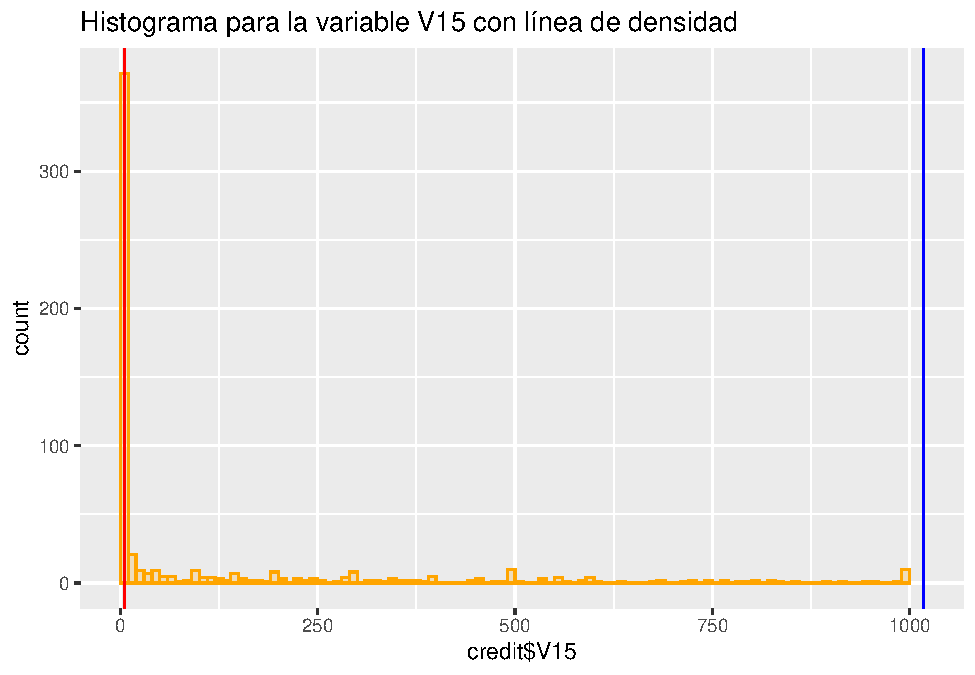
\includegraphics{PreprocesadoDeDatos_files/figure-latex/unnamed-chunk-35-1.pdf}

\hypertarget{v16}{%
\subsection{V16}\label{v16}}

Comenzamos con el análisis de la variable categórica V16, que contiene
las clases objetivo o categorías para nuestro análisis.

Ahora vamos a renombrar algunas columnas para ganar legibilidad

\begin{Shaded}
\begin{Highlighting}[]
\FunctionTok{levels}\NormalTok{(credit}\SpecialCharTok{$}\NormalTok{V16) }\OtherTok{\textless{}{-}} \FunctionTok{c}\NormalTok{(}\StringTok{"rechazada"}\NormalTok{, }\StringTok{"aprobada"}\NormalTok{)}
\end{Highlighting}
\end{Shaded}

Verificamos la estructura de V16 para confirmar que es de tipo factor y
ver las categorías presentes en la variable.

\begin{Shaded}
\begin{Highlighting}[]
\FunctionTok{str}\NormalTok{(credit}\SpecialCharTok{$}\NormalTok{V16)}
\end{Highlighting}
\end{Shaded}

\begin{verbatim}
##  Factor w/ 2 levels "rechazada","aprobada": 2 2 2 2 2 2 2 2 2 2 ...
\end{verbatim}

Calculamos el porcentaje de cada categoría en V16. Primero, usamos
table(credit\$V16) para obtener las frecuencias de cada categoría,
luego, aplicamos prop.table() para obtener la proporción relativa,
multiplicando por 100 para obtener el porcentaje.

\begin{Shaded}
\begin{Highlighting}[]
\NormalTok{porcent }\OtherTok{\textless{}{-}} \FunctionTok{prop.table}\NormalTok{(}\FunctionTok{table}\NormalTok{(credit}\SpecialCharTok{$}\NormalTok{V16)) }\SpecialCharTok{*} \DecValTok{100}
\end{Highlighting}
\end{Shaded}

Creamos una tabla combinada que incluye tanto el número total
(frecuencia) como el porcentaje de cada categoría. Usamos cbind() para
unir el total (frecuencia) y el porcentaje en una tabla.

\begin{Shaded}
\begin{Highlighting}[]
\NormalTok{porcent\_table }\OtherTok{\textless{}{-}} \FunctionTok{cbind}\NormalTok{(}\AttributeTok{total =} \FunctionTok{table}\NormalTok{(credit}\SpecialCharTok{$}\NormalTok{V16), }\AttributeTok{porcentaje =}\NormalTok{ porcent)}
\end{Highlighting}
\end{Shaded}

Mostramos el vector de porcentajes, que nos permite ver el porcentaje de
cada categoría.

\begin{Shaded}
\begin{Highlighting}[]
\NormalTok{porcent}
\end{Highlighting}
\end{Shaded}

\begin{verbatim}
## 
## rechazada  aprobada 
##  55.50725  44.49275
\end{verbatim}

Ahora que entendemos la frecuencia y proporción de cada categoría,
creamos un diagrama de sectores (o ``quesos'') para ilustrarlo de forma
gráfica.

Creamos el gráfico de sectores con pie(), donde usamos el vector de
porcentajes.

\begin{Shaded}
\begin{Highlighting}[]
\FunctionTok{pie}\NormalTok{(porcent, }\AttributeTok{main =} \StringTok{"Diagrama de Quesos para V16"}\NormalTok{, }\AttributeTok{col =} \FunctionTok{rainbow}\NormalTok{(}\FunctionTok{length}\NormalTok{(porcent)))}
\end{Highlighting}
\end{Shaded}

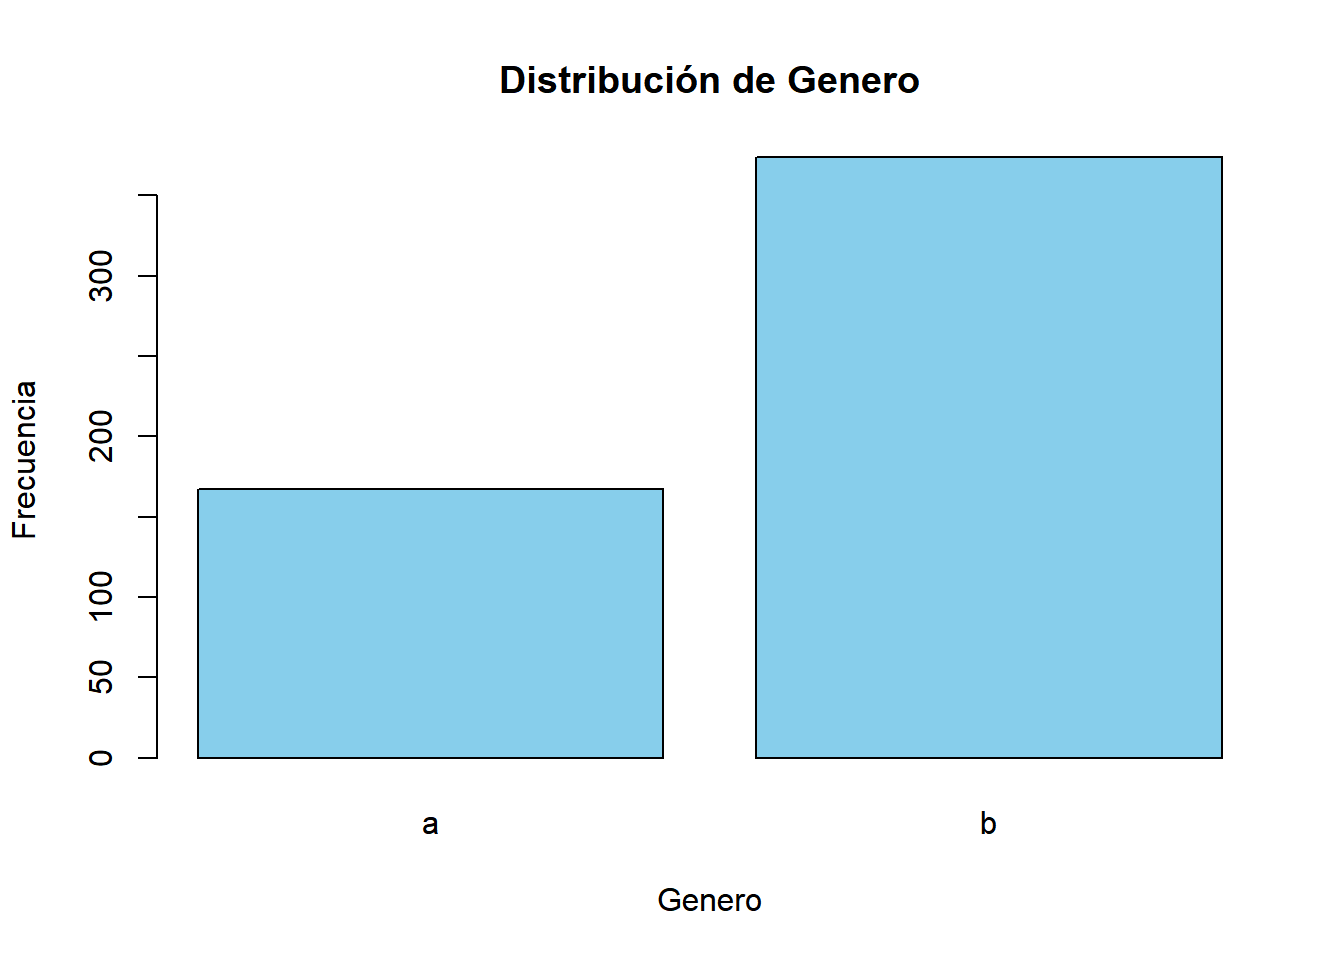
\includegraphics{PreprocesadoDeDatos_files/figure-latex/unnamed-chunk-41-1.pdf}

Con este gráfico de sectores, podemos ver visualmente la distribución de
cada categoría en V16. Dado que las categorías tienen frecuencias
similares, podemos observar que la distribución es aproximadamente
uniforme y no se identifican categorías con frecuencias extremas
(outliers).

\begin{Shaded}
\begin{Highlighting}[]
\NormalTok{melted\_data }\OtherTok{\textless{}{-}} \FunctionTok{melt}\NormalTok{(credit, }\AttributeTok{id.vars =} \StringTok{"V16"}\NormalTok{, }\AttributeTok{measure.vars =} \StringTok{"V2"}\NormalTok{, }\AttributeTok{variable.name =} \StringTok{"Variable"}\NormalTok{, }\AttributeTok{value.name =} \StringTok{"Value"}\NormalTok{)}
\NormalTok{melted\_data}
\end{Highlighting}
\end{Shaded}

\begin{verbatim}
##           V16 Variable Value
## 1    aprobada       V2 30.83
## 2    aprobada       V2 58.67
## 3    aprobada       V2 24.50
## 4    aprobada       V2 27.83
## 5    aprobada       V2 20.17
## 6    aprobada       V2 32.08
## 7    aprobada       V2 33.17
## 8    aprobada       V2 22.92
## 9    aprobada       V2 54.42
## 10   aprobada       V2 42.50
## 11   aprobada       V2 22.08
## 12   aprobada       V2 29.92
## 13   aprobada       V2 38.25
## 14   aprobada       V2 48.08
## 15   aprobada       V2 45.83
## 16   aprobada       V2 36.67
## 17   aprobada       V2 28.25
## 18   aprobada       V2 23.25
## 19   aprobada       V2 21.83
## 20   aprobada       V2 19.17
## 21   aprobada       V2 25.00
## 22   aprobada       V2 23.25
## 23   aprobada       V2 47.75
## 24   aprobada       V2 27.42
## 25   aprobada       V2 41.17
## 26   aprobada       V2 15.83
## 27   aprobada       V2 47.00
## 28   aprobada       V2 56.58
## 29   aprobada       V2 57.42
## 30   aprobada       V2 42.08
## 31   aprobada       V2 29.25
## 32   aprobada       V2 42.00
## 33   aprobada       V2 49.50
## 34   aprobada       V2 36.75
## 35   aprobada       V2 22.58
## 36   aprobada       V2 27.83
## 37   aprobada       V2 27.25
## 38   aprobada       V2 23.00
## 39   aprobada       V2 27.75
## 40   aprobada       V2 54.58
## 41   aprobada       V2 34.17
## 42   aprobada       V2 28.92
## 43   aprobada       V2 29.67
## 44   aprobada       V2 39.58
## 45   aprobada       V2 56.42
## 46   aprobada       V2 54.33
## 47   aprobada       V2 41.00
## 48   aprobada       V2 31.92
## 49   aprobada       V2 41.50
## 50   aprobada       V2 23.92
## 51   aprobada       V2 25.75
## 52   aprobada       V2 26.00
## 53   aprobada       V2 37.42
## 54   aprobada       V2 34.92
## 55   aprobada       V2 34.25
## 56   aprobada       V2 23.33
## 57   aprobada       V2 23.17
## 58   aprobada       V2 44.33
## 59   aprobada       V2 35.17
## 60   aprobada       V2 43.25
## 61   aprobada       V2 56.75
## 62   aprobada       V2 31.67
## 63   aprobada       V2 23.42
## 64   aprobada       V2 20.42
## 65   aprobada       V2 26.67
## 66   aprobada       V2 34.17
## 67   aprobada       V2 36.00
## 68   aprobada       V2 25.50
## 69   aprobada       V2 19.42
## 70   aprobada       V2 35.17
## 71  rechazada       V2 32.33
## 72  rechazada       V2 34.83
## 73  rechazada       V2 38.58
## 74  rechazada       V2 44.25
## 75  rechazada       V2 44.83
## 76  rechazada       V2 20.67
## 77  rechazada       V2 34.08
## 78  rechazada       V2 19.17
## 79  rechazada       V2 21.67
## 80  rechazada       V2 21.50
## 81  rechazada       V2 49.58
## 82  rechazada       V2 27.67
## 83  rechazada       V2 39.83
## 84  rechazada       V2    NA
## 85  rechazada       V2 27.25
## 86  rechazada       V2 37.17
## 87  rechazada       V2    NA
## 88  rechazada       V2 25.67
## 89  rechazada       V2 34.00
## 90  rechazada       V2 49.00
## 91  rechazada       V2 62.50
## 92  rechazada       V2 31.42
## 93  rechazada       V2    NA
## 94  rechazada       V2 52.33
## 95  rechazada       V2 28.75
## 96  rechazada       V2 28.58
## 97  rechazada       V2 23.00
## 98  rechazada       V2    NA
## 99  rechazada       V2 22.50
## 100 rechazada       V2 28.50
## 101 rechazada       V2 37.50
## 102 rechazada       V2 35.25
## 103 rechazada       V2 18.67
## 104 rechazada       V2 25.00
## 105 rechazada       V2 27.83
## 106 rechazada       V2 54.83
## 107 rechazada       V2 28.75
## 108 rechazada       V2 25.00
## 109 rechazada       V2 40.92
## 110 rechazada       V2 19.75
## 111 rechazada       V2 29.17
## 112 rechazada       V2 24.50
## 113 rechazada       V2 24.58
## 114 rechazada       V2 33.75
## 115 rechazada       V2 20.67
## 116 rechazada       V2 25.42
## 117 rechazada       V2 37.75
## 118  aprobada       V2 52.50
## 119  aprobada       V2 57.83
## 120  aprobada       V2 20.75
## 121  aprobada       V2 39.92
## 122  aprobada       V2 25.67
## 123  aprobada       V2 24.75
## 124  aprobada       V2 44.17
## 125  aprobada       V2 23.50
## 126  aprobada       V2 34.92
## 127  aprobada       V2 47.67
## 128  aprobada       V2 22.75
## 129  aprobada       V2 34.42
## 130  aprobada       V2 28.42
## 131  aprobada       V2 67.75
## 132  aprobada       V2 20.42
## 133  aprobada       V2 47.42
## 134  aprobada       V2 36.25
## 135  aprobada       V2 32.67
## 136  aprobada       V2 48.58
## 137  aprobada       V2 39.92
## 138  aprobada       V2 33.58
## 139  aprobada       V2 18.83
## 140  aprobada       V2 26.92
## 141  aprobada       V2 31.25
## 142  aprobada       V2 56.50
## 143  aprobada       V2 43.00
## 144  aprobada       V2 22.33
## 145  aprobada       V2 27.25
## 146  aprobada       V2 32.83
## 147  aprobada       V2 23.25
## 148  aprobada       V2 40.33
## 149  aprobada       V2 30.50
## 150  aprobada       V2 52.83
## 151  aprobada       V2 46.67
## 152  aprobada       V2 58.33
## 153  aprobada       V2 37.33
## 154  aprobada       V2 23.08
## 155  aprobada       V2 32.75
## 156  aprobada       V2 21.67
## 157  aprobada       V2 28.50
## 158  aprobada       V2 68.67
## 159  aprobada       V2 28.00
## 160  aprobada       V2 34.08
## 161  aprobada       V2 27.67
## 162  aprobada       V2 44.00
## 163  aprobada       V2 25.08
## 164  aprobada       V2 32.00
## 165  aprobada       V2 60.58
## 166  aprobada       V2 40.83
## 167  aprobada       V2 19.33
## 168  aprobada       V2 32.33
## 169  aprobada       V2 36.67
## 170  aprobada       V2 37.50
## 171  aprobada       V2 25.08
## 172  aprobada       V2 41.33
## 173  aprobada       V2 56.00
## 174  aprobada       V2 49.83
## 175  aprobada       V2 22.67
## 176  aprobada       V2 27.00
## 177  aprobada       V2 25.00
## 178  aprobada       V2 26.08
## 179  aprobada       V2 18.42
## 180  aprobada       V2 20.17
## 181  aprobada       V2 47.67
## 182  aprobada       V2 21.25
## 183  aprobada       V2 20.67
## 184  aprobada       V2 57.08
## 185  aprobada       V2 22.42
## 186  aprobada       V2 48.75
## 187  aprobada       V2 40.00
## 188  aprobada       V2 40.58
## 189  aprobada       V2 28.67
## 190  aprobada       V2 33.08
## 191  aprobada       V2 21.33
## 192  aprobada       V2 42.00
## 193  aprobada       V2 41.75
## 194  aprobada       V2 22.67
## 195  aprobada       V2 34.50
## 196  aprobada       V2 28.25
## 197  aprobada       V2 33.17
## 198  aprobada       V2 48.17
## 199  aprobada       V2 27.58
## 200  aprobada       V2 22.58
## 201  aprobada       V2 24.08
## 202  aprobada       V2 41.33
## 203  aprobada       V2 24.83
## 204  aprobada       V2 20.75
## 205  aprobada       V2 36.33
## 206  aprobada       V2 35.42
## 207  aprobada       V2 71.58
## 208  aprobada       V2 28.67
## 209  aprobada       V2 35.17
## 210  aprobada       V2 39.50
## 211  aprobada       V2 39.33
## 212  aprobada       V2 24.33
## 213  aprobada       V2 60.08
## 214  aprobada       V2 23.08
## 215  aprobada       V2 26.67
## 216  aprobada       V2 48.17
## 217  aprobada       V2 41.17
## 218  aprobada       V2 55.92
## 219  aprobada       V2 53.92
## 220  aprobada       V2 18.92
## 221  aprobada       V2 50.08
## 222  aprobada       V2 65.42
## 223  aprobada       V2 17.58
## 224  aprobada       V2 18.83
## 225  aprobada       V2 37.75
## 226  aprobada       V2 23.25
## 227  aprobada       V2 18.08
## 228  aprobada       V2 22.50
## 229  aprobada       V2 19.67
## 230  aprobada       V2 22.08
## 231  aprobada       V2 25.17
## 232  aprobada       V2 47.42
## 233  aprobada       V2 33.50
## 234  aprobada       V2 27.67
## 235  aprobada       V2 58.42
## 236  aprobada       V2 20.67
## 237  aprobada       V2 26.17
## 238  aprobada       V2 21.33
## 239  aprobada       V2 42.83
## 240  aprobada       V2 38.17
## 241  aprobada       V2 20.50
## 242  aprobada       V2 48.25
## 243  aprobada       V2 28.33
## 244  aprobada       V2 18.75
## 245  aprobada       V2 18.50
## 246  aprobada       V2 33.17
## 247  aprobada       V2 45.00
## 248  aprobada       V2 19.67
## 249  aprobada       V2 24.50
## 250  aprobada       V2 21.83
## 251  aprobada       V2 40.25
## 252  aprobada       V2 41.42
## 253  aprobada       V2 17.83
## 254  aprobada       V2 23.17
## 255 rechazada       V2    NA
## 256 rechazada       V2 18.17
## 257 rechazada       V2 20.00
## 258 rechazada       V2 20.00
## 259 rechazada       V2 20.75
## 260 rechazada       V2 24.50
## 261 rechazada       V2 32.75
## 262 rechazada       V2 52.17
## 263 rechazada       V2 48.17
## 264 rechazada       V2 20.42
## 265 rechazada       V2 50.75
## 266 rechazada       V2 17.08
## 267 rechazada       V2 18.33
## 268 rechazada       V2 32.00
## 269  aprobada       V2 59.67
## 270  aprobada       V2 18.00
## 271  aprobada       V2 37.58
## 272 rechazada       V2 32.33
## 273 rechazada       V2 18.08
## 274 rechazada       V2 38.25
## 275 rechazada       V2 30.67
## 276 rechazada       V2 18.58
## 277 rechazada       V2 19.17
## 278 rechazada       V2 18.17
## 279 rechazada       V2 24.58
## 280 rechazada       V2 16.25
## 281 rechazada       V2 21.17
## 282 rechazada       V2 23.92
## 283 rechazada       V2 17.67
## 284 rechazada       V2 16.50
## 285 rechazada       V2 23.25
## 286 rechazada       V2 17.58
## 287 rechazada       V2    NA
## 288 rechazada       V2 29.50
## 289 rechazada       V2 18.83
## 290 rechazada       V2 21.75
## 291 rechazada       V2 23.00
## 292 rechazada       V2 18.25
## 293 rechazada       V2 25.42
## 294 rechazada       V2 35.75
## 295 rechazada       V2 16.08
## 296 rechazada       V2 31.92
## 297 rechazada       V2 69.17
## 298 rechazada       V2 32.92
## 299 rechazada       V2 16.33
## 300 rechazada       V2 22.17
## 301 rechazada       V2 57.58
## 302 rechazada       V2 18.25
## 303 rechazada       V2 23.42
## 304 rechazada       V2 15.92
## 305 rechazada       V2 24.75
## 306 rechazada       V2 48.75
## 307 rechazada       V2 23.50
## 308 rechazada       V2 18.58
## 309 rechazada       V2 27.75
## 310 rechazada       V2 31.75
## 311 rechazada       V2 24.83
## 312 rechazada       V2 19.00
## 313 rechazada       V2 16.33
## 314 rechazada       V2 18.58
## 315 rechazada       V2 16.25
## 316 rechazada       V2 23.00
## 317 rechazada       V2 21.17
## 318  aprobada       V2 17.50
## 319  aprobada       V2 19.17
## 320  aprobada       V2 36.75
## 321  aprobada       V2 21.25
## 322  aprobada       V2 18.08
## 323  aprobada       V2 33.67
## 324  aprobada       V2 48.58
## 325 rechazada       V2 33.67
## 326 rechazada       V2 29.50
## 327 rechazada       V2 30.17
## 328 rechazada       V2 40.83
## 329 rechazada       V2 34.83
## 330 rechazada       V2    NA
## 331 rechazada       V2 20.42
## 332 rechazada       V2 33.25
## 333 rechazada       V2 34.08
## 334 rechazada       V2 25.25
## 335 rechazada       V2 34.75
## 336 rechazada       V2 27.67
## 337 rechazada       V2 47.33
## 338 rechazada       V2 34.83
## 339 rechazada       V2 33.25
## 340 rechazada       V2 28.00
## 341 rechazada       V2 39.08
## 342 rechazada       V2 42.75
## 343 rechazada       V2 26.92
## 344 rechazada       V2 33.75
## 345 rechazada       V2 38.92
## 346 rechazada       V2 62.75
## 347 rechazada       V2 32.25
## 348 rechazada       V2 26.75
## 349 rechazada       V2 63.33
## 350 rechazada       V2 27.83
## 351 rechazada       V2 26.17
## 352 rechazada       V2 22.17
## 353 rechazada       V2 22.50
## 354 rechazada       V2 30.75
## 355 rechazada       V2 36.67
## 356 rechazada       V2 16.00
## 357 rechazada       V2 41.17
## 358 rechazada       V2 19.50
## 359 rechazada       V2 32.42
## 360 rechazada       V2 36.75
## 361 rechazada       V2 30.25
## 362 rechazada       V2 23.08
## 363 rechazada       V2 26.83
## 364 rechazada       V2 16.92
## 365 rechazada       V2 24.42
## 366 rechazada       V2 42.83
## 367 rechazada       V2 22.75
## 368 rechazada       V2 39.42
## 369 rechazada       V2 23.58
## 370 rechazada       V2 21.42
## 371 rechazada       V2 33.00
## 372 rechazada       V2 26.33
## 373 rechazada       V2 45.00
## 374 rechazada       V2 26.25
## 375 rechazada       V2 28.17
## 376 rechazada       V2 20.83
## 377 rechazada       V2 28.67
## 378 rechazada       V2 20.67
## 379 rechazada       V2 34.42
## 380 rechazada       V2 33.58
## 381 rechazada       V2 43.17
## 382 rechazada       V2 22.67
## 383 rechazada       V2 24.33
## 384 rechazada       V2 56.83
## 385 rechazada       V2 22.08
## 386 rechazada       V2 34.00
## 387 rechazada       V2 22.58
## 388 rechazada       V2 21.17
## 389 rechazada       V2 26.67
## 390 rechazada       V2 22.92
## 391 rechazada       V2 15.17
## 392 rechazada       V2 39.92
## 393 rechazada       V2 27.42
## 394 rechazada       V2 24.75
## 395 rechazada       V2 41.17
## 396 rechazada       V2 33.08
## 397 rechazada       V2 29.83
## 398 rechazada       V2 23.58
## 399 rechazada       V2 26.17
## 400 rechazada       V2 31.00
## 401 rechazada       V2 20.75
## 402 rechazada       V2 28.92
## 403 rechazada       V2 51.92
## 404 rechazada       V2 22.67
## 405 rechazada       V2 34.00
## 406 rechazada       V2 69.50
## 407 rechazada       V2 40.33
## 408 rechazada       V2 19.58
## 409 rechazada       V2 16.00
## 410 rechazada       V2 17.08
## 411 rechazada       V2 31.25
## 412 rechazada       V2 25.17
## 413 rechazada       V2 22.67
## 414 rechazada       V2 40.58
## 415 rechazada       V2 22.25
## 416 rechazada       V2 22.25
## 417 rechazada       V2 22.50
## 418 rechazada       V2 23.58
## 419 rechazada       V2 38.42
## 420 rechazada       V2 26.58
## 421 rechazada       V2 35.00
## 422 rechazada       V2 20.42
## 423 rechazada       V2 29.42
## 424 rechazada       V2 26.17
## 425 rechazada       V2 33.67
## 426 rechazada       V2 24.58
## 427 rechazada       V2 27.67
## 428 rechazada       V2 37.50
## 429 rechazada       V2 49.17
## 430 rechazada       V2 33.58
## 431 rechazada       V2 51.83
## 432 rechazada       V2 22.92
## 433 rechazada       V2 21.83
## 434 rechazada       V2 25.25
## 435 rechazada       V2 58.58
## 436 rechazada       V2 19.00
## 437 rechazada       V2 19.58
## 438 rechazada       V2 53.33
## 439 rechazada       V2 27.17
## 440 rechazada       V2 25.92
## 441 rechazada       V2 23.08
## 442 rechazada       V2 39.58
## 443 rechazada       V2 30.58
## 444 rechazada       V2 17.25
## 445 rechazada       V2 17.67
## 446 rechazada       V2    NA
## 447 rechazada       V2 16.50
## 448 rechazada       V2 27.33
## 449 rechazada       V2 31.25
## 450 rechazada       V2 20.00
## 451 rechazada       V2    NA
## 452 rechazada       V2 39.50
## 453 rechazada       V2 36.50
## 454 rechazada       V2 29.75
## 455 rechazada       V2 52.42
## 456 rechazada       V2 36.17
## 457 rechazada       V2 34.58
## 458 rechazada       V2 29.67
## 459 rechazada       V2 36.17
## 460 rechazada       V2 25.67
## 461 rechazada       V2 24.50
## 462 rechazada       V2 24.08
## 463 rechazada       V2 21.92
## 464 rechazada       V2 36.58
## 465 rechazada       V2 23.00
## 466 rechazada       V2 27.58
## 467 rechazada       V2 31.08
## 468 rechazada       V2 30.42
## 469 rechazada       V2 22.08
## 470 rechazada       V2 16.33
## 471 rechazada       V2 21.92
## 472 rechazada       V2 21.08
## 473 rechazada       V2 17.42
## 474 rechazada       V2 19.17
## 475 rechazada       V2 20.67
## 476 rechazada       V2 26.75
## 477 rechazada       V2 23.58
## 478 rechazada       V2 39.17
## 479 rechazada       V2 22.75
## 480 rechazada       V2 26.50
## 481 rechazada       V2 16.92
## 482 rechazada       V2 23.50
## 483 rechazada       V2 17.33
## 484 rechazada       V2 23.75
## 485 rechazada       V2 34.67
## 486 rechazada       V2 74.83
## 487 rechazada       V2 28.17
## 488 rechazada       V2 24.50
## 489 rechazada       V2 18.83
## 490 rechazada       V2 45.33
## 491  aprobada       V2 47.25
## 492  aprobada       V2 24.17
## 493  aprobada       V2 39.25
## 494  aprobada       V2 20.50
## 495  aprobada       V2 18.83
## 496  aprobada       V2 19.17
## 497  aprobada       V2 25.00
## 498  aprobada       V2 20.17
## 499  aprobada       V2 25.75
## 500  aprobada       V2 20.42
## 501  aprobada       V2    NA
## 502  aprobada       V2 39.00
## 503  aprobada       V2 64.08
## 504  aprobada       V2 28.25
## 505  aprobada       V2 28.75
## 506  aprobada       V2 31.33
## 507  aprobada       V2 18.92
## 508  aprobada       V2 24.75
## 509  aprobada       V2 30.67
## 510  aprobada       V2 21.00
## 511  aprobada       V2 13.75
## 512  aprobada       V2 46.00
## 513  aprobada       V2 44.33
## 514  aprobada       V2 20.25
## 515  aprobada       V2 22.67
## 516  aprobada       V2    NA
## 517  aprobada       V2 60.92
## 518  aprobada       V2 16.08
## 519  aprobada       V2 28.17
## 520  aprobada       V2 39.17
## 521  aprobada       V2 20.42
## 522  aprobada       V2 30.00
## 523  aprobada       V2 22.83
## 524 rechazada       V2 22.50
## 525 rechazada       V2 28.58
## 526 rechazada       V2 45.17
## 527 rechazada       V2 41.58
## 528 rechazada       V2 57.08
## 529 rechazada       V2 55.75
## 530 rechazada       V2 43.25
## 531 rechazada       V2 25.33
## 532 rechazada       V2 24.58
## 533 rechazada       V2 43.17
## 534 rechazada       V2 40.92
## 535 rechazada       V2 31.83
## 536 rechazada       V2 33.92
## 537 rechazada       V2 24.92
## 538 rechazada       V2 35.25
## 539 rechazada       V2 34.25
## 540 rechazada       V2 80.25
## 541 rechazada       V2 19.42
## 542 rechazada       V2 42.75
## 543 rechazada       V2 19.67
## 544 rechazada       V2 36.33
## 545 rechazada       V2 30.08
## 546 rechazada       V2 44.25
## 547 rechazada       V2 23.58
## 548  aprobada       V2 23.92
## 549  aprobada       V2 33.17
## 550  aprobada       V2 48.33
## 551  aprobada       V2 76.75
## 552  aprobada       V2 51.33
## 553  aprobada       V2 34.75
## 554  aprobada       V2 38.58
## 555  aprobada       V2 22.42
## 556  aprobada       V2 41.92
## 557  aprobada       V2 29.58
## 558  aprobada       V2 32.17
## 559  aprobada       V2 51.42
## 560  aprobada       V2 22.83
## 561  aprobada       V2 25.00
## 562  aprobada       V2 26.75
## 563  aprobada       V2 23.33
## 564  aprobada       V2 24.42
## 565  aprobada       V2 42.17
## 566  aprobada       V2 20.83
## 567  aprobada       V2 23.08
## 568  aprobada       V2 25.17
## 569  aprobada       V2 43.08
## 570  aprobada       V2 35.75
## 571  aprobada       V2 59.50
## 572  aprobada       V2 21.00
## 573  aprobada       V2 21.92
## 574  aprobada       V2 65.17
## 575  aprobada       V2 20.33
## 576  aprobada       V2 32.25
## 577  aprobada       V2 30.17
## 578  aprobada       V2 25.17
## 579  aprobada       V2 39.17
## 580  aprobada       V2 39.08
## 581  aprobada       V2 31.67
## 582  aprobada       V2 41.00
## 583  aprobada       V2 48.50
## 584  aprobada       V2 32.67
## 585  aprobada       V2 28.08
## 586  aprobada       V2 73.42
## 587  aprobada       V2 64.08
## 588  aprobada       V2 51.58
## 589  aprobada       V2 26.67
## 590  aprobada       V2 25.33
## 591  aprobada       V2 30.17
## 592  aprobada       V2 27.00
## 593  aprobada       V2 23.17
## 594  aprobada       V2 34.17
## 595  aprobada       V2 38.67
## 596  aprobada       V2 25.75
## 597  aprobada       V2 46.08
## 598  aprobada       V2 21.50
## 599  aprobada       V2 20.08
## 600  aprobada       V2 20.50
## 601  aprobada       V2 29.50
## 602 rechazada       V2 42.25
## 603 rechazada       V2 29.83
## 604 rechazada       V2 20.08
## 605 rechazada       V2 23.42
## 606 rechazada       V2 29.58
## 607  aprobada       V2 16.17
## 608 rechazada       V2 32.33
## 609 rechazada       V2    NA
## 610 rechazada       V2 47.83
## 611 rechazada       V2 20.00
## 612 rechazada       V2 27.58
## 613 rechazada       V2 22.00
## 614 rechazada       V2 19.33
## 615 rechazada       V2 38.33
## 616 rechazada       V2 29.42
## 617 rechazada       V2 22.67
## 618 rechazada       V2 32.25
## 619 rechazada       V2 29.58
## 620 rechazada       V2 18.42
## 621 rechazada       V2 22.17
## 622  aprobada       V2 22.67
## 623  aprobada       V2 25.58
## 624 rechazada       V2 18.83
## 625 rechazada       V2 21.58
## 626 rechazada       V2 23.75
## 627 rechazada       V2 22.00
## 628 rechazada       V2 36.08
## 629 rechazada       V2 29.25
## 630 rechazada       V2 19.58
## 631 rechazada       V2 22.92
## 632 rechazada       V2 27.25
## 633 rechazada       V2 38.75
## 634 rechazada       V2 32.42
## 635 rechazada       V2 23.75
## 636 rechazada       V2 18.17
## 637 rechazada       V2 40.92
## 638 rechazada       V2 19.50
## 639 rechazada       V2 28.58
## 640 rechazada       V2 35.58
## 641 rechazada       V2 34.17
## 642 rechazada       V2 33.17
## 643 rechazada       V2 31.58
## 644 rechazada       V2 52.50
## 645 rechazada       V2 36.17
## 646 rechazada       V2 37.33
## 647 rechazada       V2 20.83
## 648 rechazada       V2 24.08
## 649 rechazada       V2 25.58
## 650 rechazada       V2 35.17
## 651 rechazada       V2 48.08
## 652 rechazada       V2 15.83
## 653 rechazada       V2 22.50
## 654 rechazada       V2 21.50
## 655 rechazada       V2 23.58
## 656 rechazada       V2 21.08
## 657 rechazada       V2 25.67
## 658 rechazada       V2 38.92
## 659 rechazada       V2 15.75
## 660 rechazada       V2 28.58
## 661 rechazada       V2 22.25
## 662 rechazada       V2 29.83
## 663 rechazada       V2 23.50
## 664 rechazada       V2 32.08
## 665 rechazada       V2 31.08
## 666 rechazada       V2 31.83
## 667 rechazada       V2 21.75
## 668 rechazada       V2 17.92
## 669 rechazada       V2 30.33
## 670 rechazada       V2 51.83
## 671 rechazada       V2 47.17
## 672 rechazada       V2 25.83
## 673 rechazada       V2 50.25
## 674 rechazada       V2 29.50
## 675 rechazada       V2 37.33
## 676 rechazada       V2 41.58
## 677 rechazada       V2 30.58
## 678 rechazada       V2 19.42
## 679 rechazada       V2 17.92
## 680 rechazada       V2 20.08
## 681 rechazada       V2 19.50
## 682 rechazada       V2 27.83
## 683 rechazada       V2 17.08
## 684 rechazada       V2 36.42
## 685 rechazada       V2 40.58
## 686 rechazada       V2 21.08
## 687 rechazada       V2 22.67
## 688 rechazada       V2 25.25
## 689 rechazada       V2 17.92
## 690 rechazada       V2 35.00
\end{verbatim}

\begin{Shaded}
\begin{Highlighting}[]
\FunctionTok{ggplot}\NormalTok{(melted\_data, }\FunctionTok{aes}\NormalTok{(}\AttributeTok{x =}\NormalTok{ V16, }\AttributeTok{y =}\NormalTok{ Value)) }\SpecialCharTok{+}
  \FunctionTok{geom\_boxplot}\NormalTok{() }\SpecialCharTok{+}
  \FunctionTok{xlab}\NormalTok{(}\StringTok{"Categoría de V16"}\NormalTok{) }\SpecialCharTok{+}
  \FunctionTok{ylab}\NormalTok{(}\StringTok{"Valores de V2"}\NormalTok{) }\SpecialCharTok{+}
  \FunctionTok{ggtitle}\NormalTok{(}\StringTok{"Distribución de V2 por Categoría de V16"}\NormalTok{)}
\end{Highlighting}
\end{Shaded}

\begin{verbatim}
## Warning: Removed 12 rows containing non-finite outside the scale range
## (`stat_boxplot()`).
\end{verbatim}

\includegraphics{PreprocesadoDeDatos_files/figure-latex/unnamed-chunk-42-1.pdf}

Observando el boxplot podemos decir que ambos tienen una distribución
simétrica. En cuanto a los outliners, no hay en exceso (en rechazada
algo más).

Ambas tienen un sesgo positivo, ya que los bigotes superiores tienen
mayor longitud.

\begin{Shaded}
\begin{Highlighting}[]
\CommentTok{\# Gráfico de densidad ajustado}
\FunctionTok{ggplot}\NormalTok{(}\AttributeTok{data =}\NormalTok{ melted\_data, }\FunctionTok{aes}\NormalTok{(}\AttributeTok{x =}\NormalTok{ Value, }\AttributeTok{color =}\NormalTok{ V16, }\AttributeTok{fill =}\NormalTok{ V16)) }\SpecialCharTok{+}
  \FunctionTok{geom\_density}\NormalTok{(}\AttributeTok{alpha =} \FloatTok{0.6}\NormalTok{) }\SpecialCharTok{+}
  \FunctionTok{scale\_fill\_discrete}\NormalTok{() }\SpecialCharTok{+}
  \FunctionTok{scale\_color\_discrete}\NormalTok{() }\SpecialCharTok{+}
  \FunctionTok{ylab}\NormalTok{(}\StringTok{"Densidad"}\NormalTok{) }\SpecialCharTok{+}  \CommentTok{\# Etiqueta para el eje y}
  \FunctionTok{xlab}\NormalTok{(}\StringTok{"Valores"}\NormalTok{) }\SpecialCharTok{+}   \CommentTok{\# Etiqueta para el eje x}
  \FunctionTok{ggtitle}\NormalTok{(}\StringTok{"Densidad de Valores por Especie"}\NormalTok{)  }\CommentTok{\# Título del gráfico}
\end{Highlighting}
\end{Shaded}

\begin{verbatim}
## Warning: Removed 12 rows containing non-finite outside the scale range
## (`stat_density()`).
\end{verbatim}

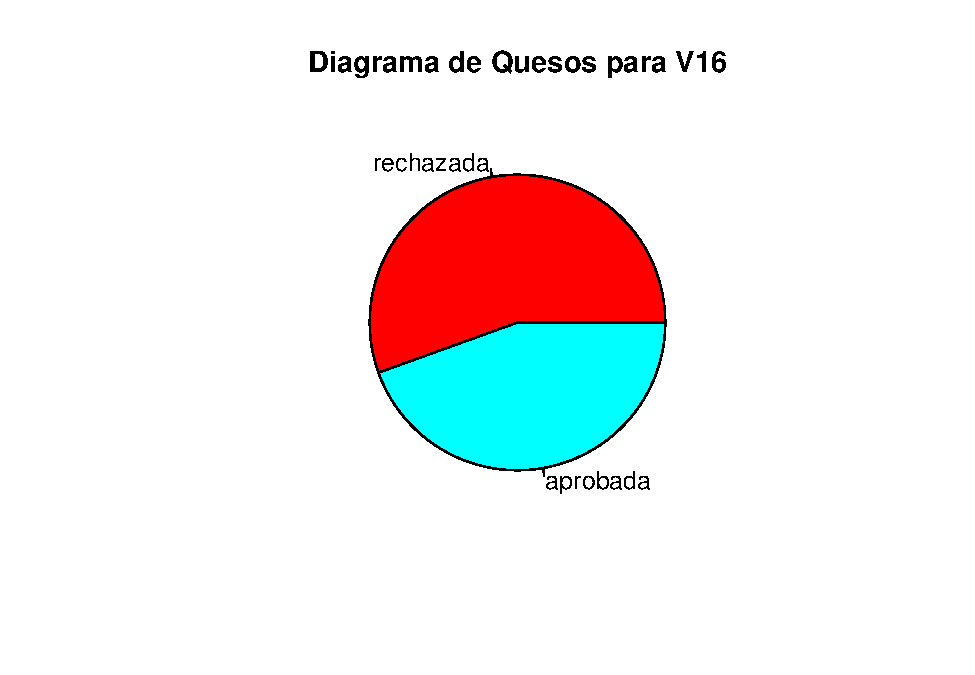
\includegraphics{PreprocesadoDeDatos_files/figure-latex/unnamed-chunk-43-1.pdf}

El análisis de la distribución de V2 muestra que ambas categorías
(rechazada y aprobada) presentan una asimetría positiva, con picos de
densidad más altos en valores bajos y una cola extendida hacia la
derecha. La curva de las solicitudes rechazadas tiene una densidad más
pronunciada cerca de los valores bajos (alrededor de 20), mientras que
la curva de las solicitudes aprobadas es más dispersa y se extiende
hacia valores más altos, sugiriendo que las aprobaciones están asociadas
con un rango más amplio de valores.

La superposición de las dos curvas, especialmente en el rango bajo de
V2, indica que esta variable por sí sola no es un fuerte discriminante
entre aprobaciones y rechazos. Sin embargo, a medida que los valores de
V2 aumentan, las aprobaciones se vuelven más frecuentes.

En resumen, V2 parece influir en la decisión de crédito, pero debido a
la considerable superposición, podría requerir análisis adicionales
junto con otras variables para mejorar la capacidad predictiva.

\begin{Shaded}
\begin{Highlighting}[]
\CommentTok{\# Boxplot chetados con puntos}
\FunctionTok{ggplot}\NormalTok{(melted\_data, }\FunctionTok{aes}\NormalTok{(}\AttributeTok{x =}\NormalTok{ V16, }\AttributeTok{y =}\NormalTok{ Value, }\AttributeTok{color=}\NormalTok{V16, }\AttributeTok{fill=}\NormalTok{V16)) }\SpecialCharTok{+}
  \FunctionTok{geom\_boxplot}\NormalTok{(}\AttributeTok{alpha=}\FloatTok{0.6}\NormalTok{) }\SpecialCharTok{+}
  \FunctionTok{geom\_jitter}\NormalTok{(}\AttributeTok{color=}\StringTok{"black"}\NormalTok{) }\SpecialCharTok{+}
  \FunctionTok{scale\_fill\_discrete}\NormalTok{() }\SpecialCharTok{+}
  \FunctionTok{scale\_color\_discrete}\NormalTok{() }\SpecialCharTok{+}
  \FunctionTok{xlab}\NormalTok{(}\StringTok{"Categoría de V16"}\NormalTok{) }\SpecialCharTok{+}
  \FunctionTok{ylab}\NormalTok{(}\StringTok{"Valores de V2"}\NormalTok{) }\SpecialCharTok{+}
  \FunctionTok{ggtitle}\NormalTok{(}\StringTok{"Distribución de V2 por Categoría de V16"}\NormalTok{)}
\end{Highlighting}
\end{Shaded}

\begin{verbatim}
## Warning: Removed 12 rows containing non-finite outside the scale range
## (`stat_boxplot()`).
\end{verbatim}

\begin{verbatim}
## Warning: Removed 12 rows containing missing values or values outside the scale range
## (`geom_point()`).
\end{verbatim}

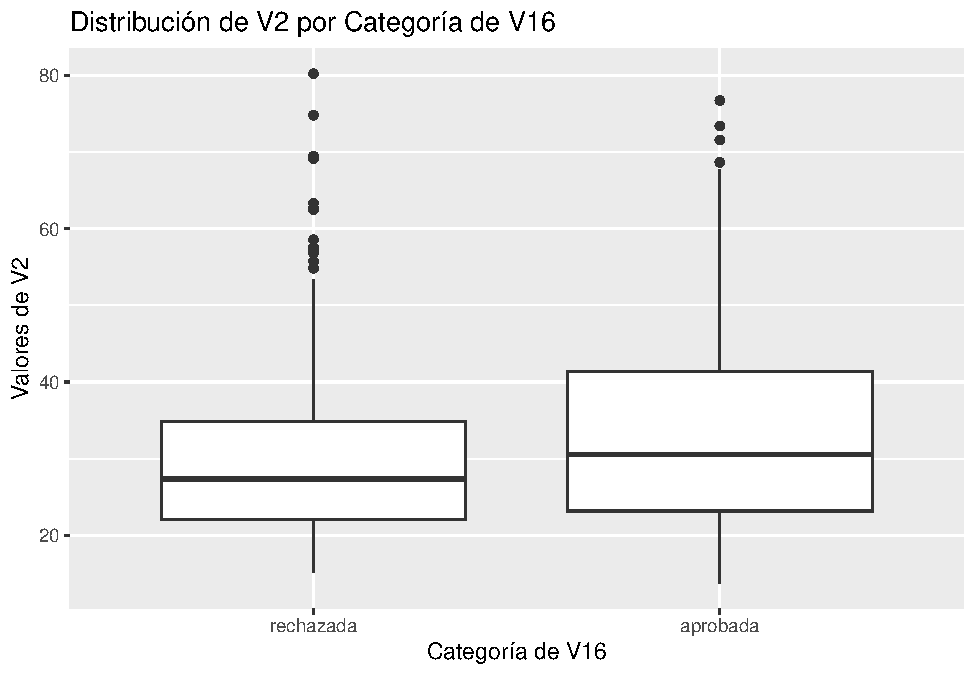
\includegraphics{PreprocesadoDeDatos_files/figure-latex/unnamed-chunk-44-1.pdf}

\hypertarget{analisis-multivariable}{%
\section{Analisis multivariable}\label{analisis-multivariable}}

\hypertarget{v16-v9}{%
\subsection{V16 V9}\label{v16-v9}}

\begin{Shaded}
\begin{Highlighting}[]
\NormalTok{melted\_data }\OtherTok{\textless{}{-}} \FunctionTok{melt}\NormalTok{(credit, }\AttributeTok{id.vars =} \StringTok{"V16"}\NormalTok{, }\AttributeTok{measure.vars =} \StringTok{"V9"}\NormalTok{, }\AttributeTok{variable.name =} \StringTok{"Variable"}\NormalTok{, }\AttributeTok{value.name =} \StringTok{"Value"}\NormalTok{)}

\FunctionTok{ggplot}\NormalTok{(melted\_data, }\FunctionTok{aes}\NormalTok{(}\AttributeTok{x =}\NormalTok{ V16, }\AttributeTok{y =}\NormalTok{ Value)) }\SpecialCharTok{+}
  \FunctionTok{geom\_boxplot}\NormalTok{() }\SpecialCharTok{+}
  \FunctionTok{xlab}\NormalTok{(}\StringTok{"Categoría de V16"}\NormalTok{) }\SpecialCharTok{+}
  \FunctionTok{ylab}\NormalTok{(}\StringTok{"Valores de V2"}\NormalTok{) }\SpecialCharTok{+}
  \FunctionTok{ggtitle}\NormalTok{(}\StringTok{"Distribución de V2 por Categoría de V16"}\NormalTok{)}
\end{Highlighting}
\end{Shaded}

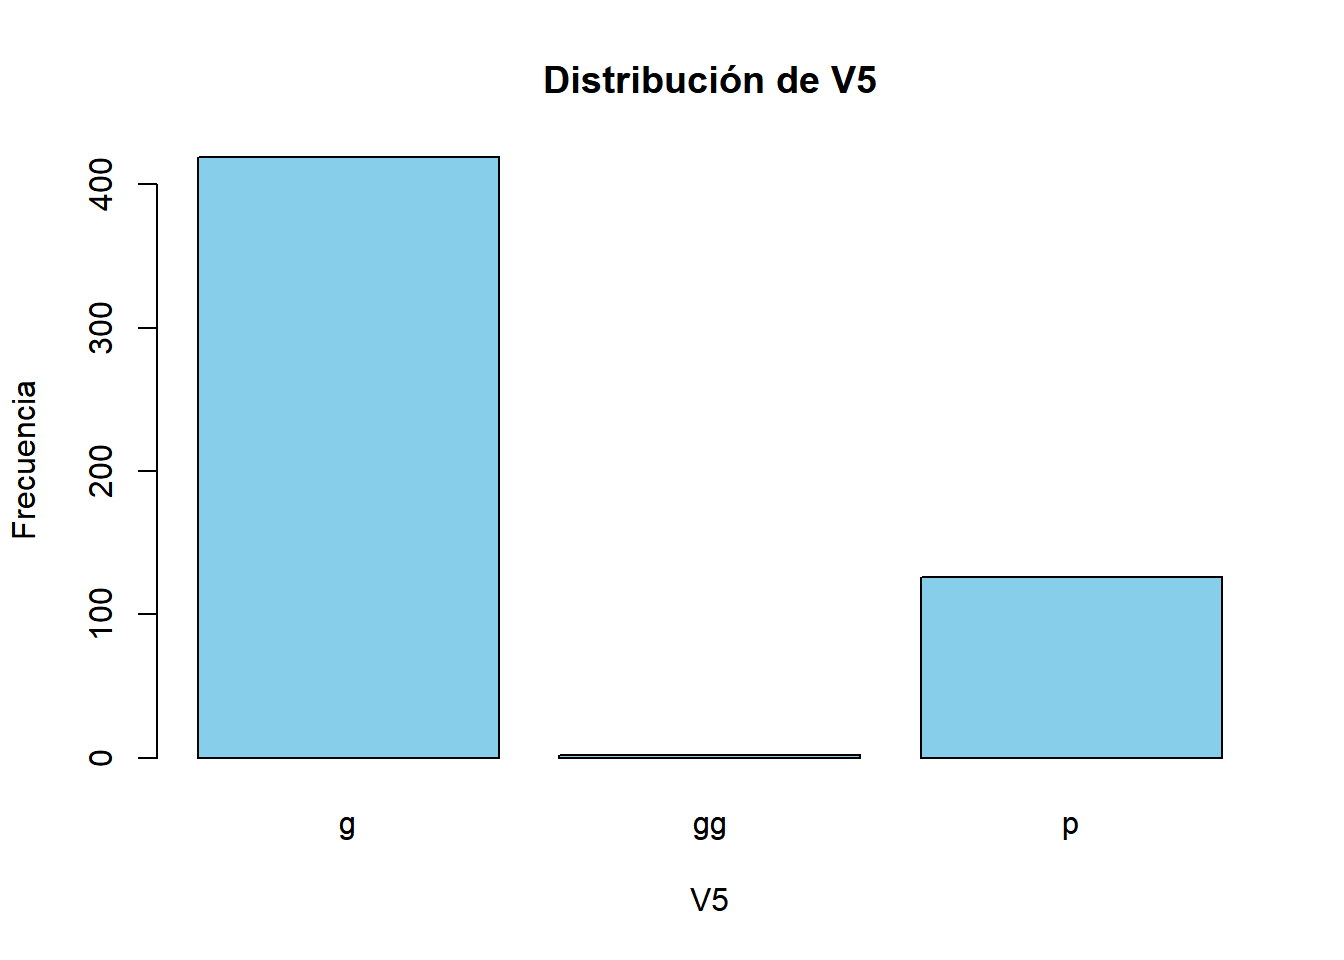
\includegraphics{PreprocesadoDeDatos_files/figure-latex/unnamed-chunk-45-1.pdf}

Observando el boxplot podemos decir que ambos tienen una distribución
simétrica. En cuanto a los outliners, no hay en exceso (en rechazada
algo más). Ambas tienen un sesgo positivo, ya que los bigotes superiores
tienen mayor longitud.

\begin{Shaded}
\begin{Highlighting}[]
\CommentTok{\# Gráfico de densidad ajustado}
\FunctionTok{ggplot}\NormalTok{(}\AttributeTok{data =}\NormalTok{ melted\_data, }\FunctionTok{aes}\NormalTok{(}\AttributeTok{x =}\NormalTok{ Value, }\AttributeTok{color =}\NormalTok{ V16, }\AttributeTok{fill =}\NormalTok{ V16)) }\SpecialCharTok{+}
  \FunctionTok{geom\_density}\NormalTok{(}\AttributeTok{alpha =} \FloatTok{0.6}\NormalTok{) }\SpecialCharTok{+}
  \FunctionTok{scale\_fill\_discrete}\NormalTok{() }\SpecialCharTok{+}
  \FunctionTok{scale\_color\_discrete}\NormalTok{() }\SpecialCharTok{+}
  \FunctionTok{ylab}\NormalTok{(}\StringTok{"Densidad"}\NormalTok{) }\SpecialCharTok{+}  \CommentTok{\# Etiqueta para el eje y}
  \FunctionTok{xlab}\NormalTok{(}\StringTok{"Valores"}\NormalTok{) }\SpecialCharTok{+}   \CommentTok{\# Etiqueta para el eje x}
  \FunctionTok{ggtitle}\NormalTok{(}\StringTok{"Densidad de Valores por Especie"}\NormalTok{)  }\CommentTok{\# Título del gráfico}
\end{Highlighting}
\end{Shaded}

\includegraphics{PreprocesadoDeDatos_files/figure-latex/unnamed-chunk-46-1.pdf}

Es interesante apreciar que hay ciertas zonas en las que se ensancha el
gráfico de aprobadas y adelgaza el gráfico de rechazadas y viceversa.
Por la relación comentada con anterioridad. Puede ser que en los
intervalos {[}0,100{]} y {[}300,500{]} aproximadamente, correspondan a
casas pertenecientes a barrios más adinerados.

\begin{Shaded}
\begin{Highlighting}[]
\CommentTok{\# Convertir automáticamente columnas de tipo \textquotesingle{}chr\textquotesingle{} a \textquotesingle{}factor\textquotesingle{}}
\NormalTok{combined\_credit[}\FunctionTok{sapply}\NormalTok{(combined\_credit, is.character)] }\OtherTok{\textless{}{-}} \FunctionTok{lapply}\NormalTok{(combined\_credit[}\FunctionTok{sapply}\NormalTok{(combined\_credit, is.character)], as.factor)}
\end{Highlighting}
\end{Shaded}

\begin{Shaded}
\begin{Highlighting}[]
\CommentTok{\# Ahora vamos a renombrar algunas columnas para ganar legibilidad}
\FunctionTok{levels}\NormalTok{(combined\_credit}\SpecialCharTok{$}\NormalTok{V16) }\OtherTok{\textless{}{-}} \FunctionTok{c}\NormalTok{(}\StringTok{"rechazada"}\NormalTok{, }\StringTok{"aprobada"}\NormalTok{)}

\CommentTok{\# Comprobamos que no hay missing{-}data:}
\FunctionTok{sum}\NormalTok{(}\SpecialCharTok{!}\FunctionTok{complete.cases}\NormalTok{(combined\_credit))}
\end{Highlighting}
\end{Shaded}

\begin{verbatim}
## [1] 37
\end{verbatim}

\begin{Shaded}
\begin{Highlighting}[]
\CommentTok{\# De momento no haremos nada con estos 37 datos perdidos}
\end{Highlighting}
\end{Shaded}

Vamos a ver qué forma tienen nuestros datos:

\begin{Shaded}
\begin{Highlighting}[]
\FunctionTok{str}\NormalTok{(combined\_credit)}
\end{Highlighting}
\end{Shaded}

\begin{verbatim}
## 'data.frame':    690 obs. of  17 variables:
##  $ V1    : Factor w/ 2 levels "a","b": 2 2 2 2 2 1 2 2 1 2 ...
##  $ V2    : num  30.8 27.8 20.2 32.1 33.2 ...
##  $ V3    : num  0 1.54 5.62 4 1.04 ...
##  $ V4    : Factor w/ 3 levels "l","u","y": 2 2 2 2 2 2 3 3 2 3 ...
##  $ V5    : Factor w/ 3 levels "g","gg","p": 1 1 1 1 1 1 3 3 1 3 ...
##  $ V6    : Factor w/ 14 levels "aa","c","cc",..: 13 13 13 10 12 3 9 13 9 9 ...
##  $ V7    : Factor w/ 9 levels "bb","dd","ff",..: 8 8 8 8 4 8 4 8 8 8 ...
##  $ V8    : num  1.25 3.75 1.71 2.5 6.5 ...
##  $ V9    : Factor w/ 2 levels "f","t": 2 2 2 2 2 2 2 2 2 2 ...
##  $ V10   : Factor w/ 2 levels "f","t": 2 2 1 1 1 1 1 1 1 2 ...
##  $ V11   : int  1 5 0 0 0 0 0 0 0 10 ...
##  $ V12   : Factor w/ 2 levels "f","t": 1 2 1 2 2 1 1 2 2 2 ...
##  $ V13   : Factor w/ 3 levels "g","p","s": 1 1 3 1 1 1 1 1 1 1 ...
##  $ V14   : int  202 100 120 360 164 80 180 52 0 320 ...
##  $ V15   : int  0 3 0 0 31285 1349 314 1442 0 0 ...
##  $ V16   : Factor w/ 2 levels "rechazada","aprobada": 2 2 2 2 2 2 2 2 2 2 ...
##  $ Origen: Factor w/ 2 levels "test","train": 2 2 2 2 2 2 2 2 2 2 ...
\end{verbatim}

\hfill\break

\begin{Shaded}
\begin{Highlighting}[]
\CommentTok{\# Ahora vamos a renombrar algunas columnas para ganar legibilidad}
\FunctionTok{levels}\NormalTok{(combined\_credit}\SpecialCharTok{$}\NormalTok{V16) }\OtherTok{\textless{}{-}} \FunctionTok{c}\NormalTok{(}\StringTok{"rechazada"}\NormalTok{, }\StringTok{"aprobada"}\NormalTok{)}

\CommentTok{\# Comprobamos que no hay missing{-}data:}
\FunctionTok{sum}\NormalTok{(}\SpecialCharTok{!}\FunctionTok{complete.cases}\NormalTok{(combined\_credit))}
\end{Highlighting}
\end{Shaded}

\begin{verbatim}
## [1] 37
\end{verbatim}

\begin{Shaded}
\begin{Highlighting}[]
\CommentTok{\# De momento no haremos nada con estos 37 datos perdidos}
\end{Highlighting}
\end{Shaded}

Vamos a ver qué forma tienen nuestros datos:

\begin{Shaded}
\begin{Highlighting}[]
\FunctionTok{str}\NormalTok{(combined\_credit)}
\end{Highlighting}
\end{Shaded}

\begin{verbatim}
## 'data.frame':    690 obs. of  17 variables:
##  $ V1    : Factor w/ 2 levels "a","b": 2 2 2 2 2 1 2 2 1 2 ...
##  $ V2    : num  30.8 27.8 20.2 32.1 33.2 ...
##  $ V3    : num  0 1.54 5.62 4 1.04 ...
##  $ V4    : Factor w/ 3 levels "l","u","y": 2 2 2 2 2 2 3 3 2 3 ...
##  $ V5    : Factor w/ 3 levels "g","gg","p": 1 1 1 1 1 1 3 3 1 3 ...
##  $ V6    : Factor w/ 14 levels "aa","c","cc",..: 13 13 13 10 12 3 9 13 9 9 ...
##  $ V7    : Factor w/ 9 levels "bb","dd","ff",..: 8 8 8 8 4 8 4 8 8 8 ...
##  $ V8    : num  1.25 3.75 1.71 2.5 6.5 ...
##  $ V9    : Factor w/ 2 levels "f","t": 2 2 2 2 2 2 2 2 2 2 ...
##  $ V10   : Factor w/ 2 levels "f","t": 2 2 1 1 1 1 1 1 1 2 ...
##  $ V11   : int  1 5 0 0 0 0 0 0 0 10 ...
##  $ V12   : Factor w/ 2 levels "f","t": 1 2 1 2 2 1 1 2 2 2 ...
##  $ V13   : Factor w/ 3 levels "g","p","s": 1 1 3 1 1 1 1 1 1 1 ...
##  $ V14   : int  202 100 120 360 164 80 180 52 0 320 ...
##  $ V15   : int  0 3 0 0 31285 1349 314 1442 0 0 ...
##  $ V16   : Factor w/ 2 levels "rechazada","aprobada": 2 2 2 2 2 2 2 2 2 2 ...
##  $ Origen: Factor w/ 2 levels "test","train": 2 2 2 2 2 2 2 2 2 2 ...
\end{verbatim}

\hypertarget{pre-procesado-de-datos-i-tratamiento-de-outliers-y-nulos}{%
\section{Pre-procesado de datos (I): Tratamiento de outliers y
nulos:}\label{pre-procesado-de-datos-i-tratamiento-de-outliers-y-nulos}}

Comenzamos renombrando las columnas en base a la información que
tenemos:

\begin{Shaded}
\begin{Highlighting}[]
\FunctionTok{colnames}\NormalTok{(combined\_credit)[}\FunctionTok{colnames}\NormalTok{(combined\_credit) }\SpecialCharTok{==} \StringTok{"V1"}\NormalTok{] }\OtherTok{\textless{}{-}} \StringTok{"Genero"}
\FunctionTok{colnames}\NormalTok{(combined\_credit)[}\FunctionTok{colnames}\NormalTok{(combined\_credit) }\SpecialCharTok{==} \StringTok{"V2"}\NormalTok{] }\OtherTok{\textless{}{-}} \StringTok{"Edad"}
\FunctionTok{colnames}\NormalTok{(combined\_credit)[}\FunctionTok{colnames}\NormalTok{(combined\_credit) }\SpecialCharTok{==} \StringTok{"V3"}\NormalTok{] }\OtherTok{\textless{}{-}} \StringTok{"Deuda"}
\FunctionTok{colnames}\NormalTok{(combined\_credit)[}\FunctionTok{colnames}\NormalTok{(combined\_credit) }\SpecialCharTok{==} \StringTok{"V4"}\NormalTok{] }\OtherTok{\textless{}{-}} \StringTok{"EstadoCivil"}
\FunctionTok{colnames}\NormalTok{(combined\_credit)[}\FunctionTok{colnames}\NormalTok{(combined\_credit) }\SpecialCharTok{==} \StringTok{"V8"}\NormalTok{] }\OtherTok{\textless{}{-}} \StringTok{"AnyosContratado"}
\FunctionTok{colnames}\NormalTok{(combined\_credit)[}\FunctionTok{colnames}\NormalTok{(combined\_credit) }\SpecialCharTok{==} \StringTok{"V10"}\NormalTok{] }\OtherTok{\textless{}{-}} \StringTok{"Empleado"}
\FunctionTok{colnames}\NormalTok{(combined\_credit)[}\FunctionTok{colnames}\NormalTok{(combined\_credit) }\SpecialCharTok{==} \StringTok{"V11"}\NormalTok{] }\OtherTok{\textless{}{-}} \StringTok{"Solvencia"}
\FunctionTok{colnames}\NormalTok{(combined\_credit)[}\FunctionTok{colnames}\NormalTok{(combined\_credit) }\SpecialCharTok{==} \StringTok{"V13"}\NormalTok{] }\OtherTok{\textless{}{-}} \StringTok{"composicionPoblacion"}
\end{Highlighting}
\end{Shaded}

\ul{\textbf{Tratamiento de valores fuera de rango:}}

Para ello, vamos a diseñar una función que detecte outliners. Como hemos
aprendido a hacerlo es con la siguiente fórmula: si valor \textbf{∈}
{[}Q1 - 1.5 * RI, Q3 + 1.5 * RI{]} se considera outliner. Siendo RI
(Rango Intercuatil). Solo miramos el conjunto de Train para que el
conjunto de Test no se aproveche de dichos datos (p.~independecia de
conjuntos).

\begin{Shaded}
\begin{Highlighting}[]
\NormalTok{credit.Datos.Train }\OtherTok{\textless{}{-}}\NormalTok{ combined\_credit[combined\_credit}\SpecialCharTok{$}\NormalTok{Origen }\SpecialCharTok{==} \StringTok{"train"}\NormalTok{, ]}
\NormalTok{credit.Datos.Test }\OtherTok{\textless{}{-}}\NormalTok{ combined\_credit[combined\_credit}\SpecialCharTok{$}\NormalTok{Origen }\SpecialCharTok{==} \StringTok{"test"}\NormalTok{, ]}

\NormalTok{detectar\_outliers }\OtherTok{\textless{}{-}} \ControlFlowTok{function}\NormalTok{(x) \{}
\NormalTok{  Q1 }\OtherTok{\textless{}{-}} \FunctionTok{quantile}\NormalTok{(x, }\FloatTok{0.25}\NormalTok{, }\AttributeTok{na.rm =} \ConstantTok{TRUE}\NormalTok{)}
\NormalTok{  Q3 }\OtherTok{\textless{}{-}} \FunctionTok{quantile}\NormalTok{(x, }\FloatTok{0.75}\NormalTok{, }\AttributeTok{na.rm =} \ConstantTok{TRUE}\NormalTok{)}
\NormalTok{  RI }\OtherTok{\textless{}{-}}\NormalTok{ Q3 }\SpecialCharTok{{-}}\NormalTok{ Q1}
\NormalTok{  limite\_inferior }\OtherTok{\textless{}{-}}\NormalTok{ Q1 }\SpecialCharTok{{-}} \FloatTok{1.5} \SpecialCharTok{*}\NormalTok{ RI}
\NormalTok{  limite\_superior }\OtherTok{\textless{}{-}}\NormalTok{ Q3 }\SpecialCharTok{+} \FloatTok{1.5} \SpecialCharTok{*}\NormalTok{ RI}
  \FunctionTok{return}\NormalTok{(x }\SpecialCharTok{\textless{}}\NormalTok{ limite\_inferior }\SpecialCharTok{|}\NormalTok{ x }\SpecialCharTok{\textgreater{}}\NormalTok{ limite\_superior)}
\NormalTok{\}}

\NormalTok{credit.Datos.continuas }\OtherTok{\textless{}{-}}\NormalTok{ credit.Datos.Train[, }\FunctionTok{sapply}\NormalTok{(credit.Datos.Train, is.numeric)]}
\NormalTok{outliners }\OtherTok{\textless{}{-}} \FunctionTok{lapply}\NormalTok{(credit.Datos.continuas, detectar\_outliers)}

\CommentTok{\# Contar los outliers por variable}
\NormalTok{sumas\_outliners }\OtherTok{\textless{}{-}} \FunctionTok{sapply}\NormalTok{(outliners, }\ControlFlowTok{function}\NormalTok{(x) }\FunctionTok{sum}\NormalTok{(x, }\AttributeTok{na.rm =} \ConstantTok{TRUE}\NormalTok{))}
\NormalTok{sumas\_outliners}
\end{Highlighting}
\end{Shaded}

\begin{verbatim}
##            Edad           Deuda AnyosContratado       Solvencia             V14 
##              17              15              50              63               9 
##             V15 
##              79
\end{verbatim}

Sin embargo, estos datos no son tan representativos. Necesitamos saber
qué porcentaje son atípicos del total de datos.

\begin{Shaded}
\begin{Highlighting}[]
\NormalTok{numero\_filas }\OtherTok{\textless{}{-}} \FunctionTok{nrow}\NormalTok{(}\FunctionTok{na.omit}\NormalTok{(credit.Datos.Train))}

\NormalTok{proporcion }\OtherTok{\textless{}{-}} \ControlFlowTok{function}\NormalTok{(x) \{}
  \FunctionTok{return}\NormalTok{(x}\SpecialCharTok{/}\NormalTok{numero\_filas}\SpecialCharTok{*}\DecValTok{100}\NormalTok{)}
\NormalTok{\}}

\NormalTok{proporciones }\OtherTok{\textless{}{-}} \FunctionTok{lapply}\NormalTok{(sumas\_outliners, proporcion)}
\NormalTok{proporciones}
\end{Highlighting}
\end{Shaded}

\begin{verbatim}
## $Edad
## [1] 3.294574
## 
## $Deuda
## [1] 2.906977
## 
## $AnyosContratado
## [1] 9.689922
## 
## $Solvencia
## [1] 12.2093
## 
## $V14
## [1] 1.744186
## 
## $V15
## [1] 15.31008
\end{verbatim}

Según hemos estado investigando cuando el porcentaje de outliners es
superior a 5\% hay que tratarlos ya que pueden ser problemáticos. En
este caso como mucho tenemos un 15\% que es un valor alto, pero tampoco
es elevadísimo. Siendo estos: AnyosContratado, Solvencia y V15:

\begin{Shaded}
\begin{Highlighting}[]
\FunctionTok{boxplot}\NormalTok{(credit.Datos.Train}\SpecialCharTok{$}\NormalTok{AnyosContratado,}\AttributeTok{boxwex=}\FloatTok{0.15}\NormalTok{,}\AttributeTok{ylab=}\StringTok{"AnyosContratado"}\NormalTok{)}
\FunctionTok{rug}\NormalTok{(}\FunctionTok{jitter}\NormalTok{(credit.Datos.Train}\SpecialCharTok{$}\NormalTok{AnyosContratado),}\AttributeTok{side=}\DecValTok{2}\NormalTok{)}
\FunctionTok{abline}\NormalTok{(}\AttributeTok{h=}\FunctionTok{mean}\NormalTok{(credit.Datos.Train}\SpecialCharTok{$}\NormalTok{AnyosContratado,}\AttributeTok{na.rm=}\NormalTok{T),}\AttributeTok{lty=}\DecValTok{2}\NormalTok{)}
\end{Highlighting}
\end{Shaded}

\includegraphics{PreprocesadoDeDatos_files/figure-latex/unnamed-chunk-55-1.pdf}

\begin{Shaded}
\begin{Highlighting}[]
\FunctionTok{boxplot}\NormalTok{(credit.Datos.Train}\SpecialCharTok{$}\NormalTok{Solvencia,}\AttributeTok{boxwex=}\FloatTok{0.15}\NormalTok{,}\AttributeTok{ylab=}\StringTok{"Solvencia"}\NormalTok{)}
\FunctionTok{rug}\NormalTok{(}\FunctionTok{jitter}\NormalTok{(credit.Datos.Train}\SpecialCharTok{$}\NormalTok{Solvencia),}\AttributeTok{side=}\DecValTok{2}\NormalTok{)}
\FunctionTok{abline}\NormalTok{(}\AttributeTok{h=}\FunctionTok{mean}\NormalTok{(credit.Datos.Train}\SpecialCharTok{$}\NormalTok{Solvencia,}\AttributeTok{na.rm=}\NormalTok{T),}\AttributeTok{lty=}\DecValTok{2}\NormalTok{)}
\end{Highlighting}
\end{Shaded}

\includegraphics{PreprocesadoDeDatos_files/figure-latex/unnamed-chunk-55-2.pdf}

\begin{Shaded}
\begin{Highlighting}[]
\FunctionTok{boxplot}\NormalTok{(credit.Datos.Train}\SpecialCharTok{$}\NormalTok{V15,}\AttributeTok{boxwex=}\FloatTok{0.15}\NormalTok{,}\AttributeTok{ylab=}\StringTok{"V15"}\NormalTok{)}
\FunctionTok{rug}\NormalTok{(}\FunctionTok{jitter}\NormalTok{(credit.Datos.Train}\SpecialCharTok{$}\NormalTok{V15),}\AttributeTok{side=}\DecValTok{2}\NormalTok{)}
\FunctionTok{abline}\NormalTok{(}\AttributeTok{h=}\FunctionTok{mean}\NormalTok{(credit.Datos.Train}\SpecialCharTok{$}\NormalTok{V15,}\AttributeTok{na.rm=}\NormalTok{T),}\AttributeTok{lty=}\DecValTok{2}\NormalTok{)}
\end{Highlighting}
\end{Shaded}

\includegraphics{PreprocesadoDeDatos_files/figure-latex/unnamed-chunk-55-3.pdf}

Decidimos que queremos equiparar a los valores fuera de rango con los
valores extremos. Esto se llama winsorización:\\

\begin{Shaded}
\begin{Highlighting}[]
\CommentTok{\# Función para calcular límites de winsorización (IR)}
\NormalTok{calcular\_limites }\OtherTok{\textless{}{-}} \ControlFlowTok{function}\NormalTok{(x) \{}
\NormalTok{  Q1 }\OtherTok{\textless{}{-}} \FunctionTok{quantile}\NormalTok{(x, }\FloatTok{0.25}\NormalTok{, }\AttributeTok{na.rm =} \ConstantTok{TRUE}\NormalTok{)}
\NormalTok{  Q3 }\OtherTok{\textless{}{-}} \FunctionTok{quantile}\NormalTok{(x, }\FloatTok{0.75}\NormalTok{, }\AttributeTok{na.rm =} \ConstantTok{TRUE}\NormalTok{)}
\NormalTok{  RI }\OtherTok{\textless{}{-}}\NormalTok{ Q3 }\SpecialCharTok{{-}}\NormalTok{ Q1}
\NormalTok{  limite\_inferior }\OtherTok{\textless{}{-}}\NormalTok{ Q1 }\SpecialCharTok{{-}} \FloatTok{1.5} \SpecialCharTok{*}\NormalTok{ RI}
\NormalTok{  limite\_superior }\OtherTok{\textless{}{-}}\NormalTok{ Q3 }\SpecialCharTok{+} \FloatTok{1.5} \SpecialCharTok{*}\NormalTok{ RI}
  \FunctionTok{return}\NormalTok{(}\FunctionTok{c}\NormalTok{(limite\_inferior, limite\_superior))}
\NormalTok{\}}

\CommentTok{\# Función para aplicar winsorización con límites definidos}
\NormalTok{winsorizar\_con\_limites }\OtherTok{\textless{}{-}} \ControlFlowTok{function}\NormalTok{(x, limites) \{}
\NormalTok{  limite\_inferior }\OtherTok{\textless{}{-}}\NormalTok{ limites[}\DecValTok{1}\NormalTok{]}
\NormalTok{  limite\_superior }\OtherTok{\textless{}{-}}\NormalTok{ limites[}\DecValTok{2}\NormalTok{]}
\NormalTok{  x[x }\SpecialCharTok{\textless{}}\NormalTok{ limite\_inferior] }\OtherTok{\textless{}{-}}\NormalTok{ limite\_inferior}
\NormalTok{  x[x }\SpecialCharTok{\textgreater{}}\NormalTok{ limite\_superior] }\OtherTok{\textless{}{-}}\NormalTok{ limite\_superior}
  \FunctionTok{return}\NormalTok{(x)}
\NormalTok{\}}

\NormalTok{columnas\_a\_winsorizar }\OtherTok{\textless{}{-}} \FunctionTok{c}\NormalTok{(}\StringTok{"AnyosContratado"}\NormalTok{, }\StringTok{"Solvencia"}\NormalTok{, }\StringTok{"V15"}\NormalTok{)}

\NormalTok{credit.Datos.Train.wins }\OtherTok{\textless{}{-}}\NormalTok{ credit.Datos.Train}
\NormalTok{credit.Datos.Test.wins }\OtherTok{\textless{}{-}}\NormalTok{ credit.Datos.Test}

\CommentTok{\# Calcular límites en el conjunto de entrenamiento}
\NormalTok{limites\_winsorizacion }\OtherTok{\textless{}{-}} \FunctionTok{lapply}\NormalTok{(credit.Datos.Train.wins[, columnas\_a\_winsorizar], calcular\_limites)}

\CommentTok{\# Winsorizar el conjunto de entrenamiento}
\ControlFlowTok{for}\NormalTok{ (col }\ControlFlowTok{in}\NormalTok{ columnas\_a\_winsorizar) \{}
\NormalTok{  credit.Datos.Train.wins[[col]] }\OtherTok{\textless{}{-}} \FunctionTok{winsorizar\_con\_limites}\NormalTok{(credit.Datos.Train.wins[[col]], limites\_winsorizacion[[col]])}
\NormalTok{\}}

\CommentTok{\# Aplicar los mismos límites al conjunto de prueba (p. de independencia de conjuntos)}
\ControlFlowTok{for}\NormalTok{ (col }\ControlFlowTok{in}\NormalTok{ columnas\_a\_winsorizar) \{}
\NormalTok{  credit.Datos.Test.wins[[col]] }\OtherTok{\textless{}{-}} \FunctionTok{winsorizar\_con\_limites}\NormalTok{(credit.Datos.Test.wins[[col]], limites\_winsorizacion[[col]])}
\NormalTok{\}}
\end{Highlighting}
\end{Shaded}

En el caso de que NO queramos usar la winsorización solo debemos de
comentar líneas:

\begin{Shaded}
\begin{Highlighting}[]
\NormalTok{credit.Datos.Train }\OtherTok{\textless{}{-}}\NormalTok{ credit.Datos.Train.wins}
\NormalTok{credit.Datos.Test }\OtherTok{\textless{}{-}}\NormalTok{ credit.Datos.Test.wins}
\end{Highlighting}
\end{Shaded}

Comprobamos que ya no hay valores fuera de rango, excepto en ``Edad'',
``Deuda'' y ``V14'' que el porcentaje es muy bajo.

\begin{Shaded}
\begin{Highlighting}[]
\NormalTok{credit.Datos.continuas }\OtherTok{\textless{}{-}}\NormalTok{ credit.Datos.Train[, }\FunctionTok{sapply}\NormalTok{(credit.Datos.Train, is.numeric)]}
\NormalTok{outliners }\OtherTok{\textless{}{-}} \FunctionTok{lapply}\NormalTok{(credit.Datos.continuas, detectar\_outliers)}

\CommentTok{\# Contar los outliers por variable}
\NormalTok{sumas\_outliners }\OtherTok{\textless{}{-}} \FunctionTok{sapply}\NormalTok{(outliners, }\ControlFlowTok{function}\NormalTok{(x) }\FunctionTok{sum}\NormalTok{(x, }\AttributeTok{na.rm =} \ConstantTok{TRUE}\NormalTok{))}
\NormalTok{sumas\_outliners}
\end{Highlighting}
\end{Shaded}

\begin{verbatim}
##            Edad           Deuda AnyosContratado       Solvencia             V14 
##              17              15               0               0               9 
##             V15 
##               0
\end{verbatim}

Sin embargo, debemos de analizar si en ``Edad'', ``Deuda'' y ``V14'' hay
errores evidentes que puedan perjudicar el rendimiento del modelo:

\begin{Shaded}
\begin{Highlighting}[]
\FunctionTok{summary}\NormalTok{(credit.Datos.Train}\SpecialCharTok{$}\NormalTok{Edad)}
\end{Highlighting}
\end{Shaded}

\begin{verbatim}
##    Min. 1st Qu.  Median    Mean 3rd Qu.    Max.    NA's 
##   13.75   22.50   27.83   31.32   37.33   80.25      12
\end{verbatim}

\begin{Shaded}
\begin{Highlighting}[]
\FunctionTok{summary}\NormalTok{(credit.Datos.Train}\SpecialCharTok{$}\NormalTok{Deuda)}
\end{Highlighting}
\end{Shaded}

\begin{verbatim}
##    Min. 1st Qu.  Median    Mean 3rd Qu.    Max. 
##   0.000   1.000   2.750   4.795   7.500  28.000
\end{verbatim}

\begin{Shaded}
\begin{Highlighting}[]
\FunctionTok{summary}\NormalTok{(credit.Datos.Train}\SpecialCharTok{$}\NormalTok{V14)}
\end{Highlighting}
\end{Shaded}

\begin{verbatim}
##    Min. 1st Qu.  Median    Mean 3rd Qu.    Max.    NA's 
##     0.0    73.0   160.0   183.5   280.0  2000.0      13
\end{verbatim}

En Deuda y V14 no parece que haya valores incorrectos. Sobre todo en
Deuda no parece que haya nada raro, en cuanto a V14 no podemos decir
mucho ya que no conocemos (especulado) su significado.

Sin embargo en Edad nos podemos dar cuenta que hay valores erroneos, ya
que los menores de edad en Estados Unidos no pueden solicitar créditos.
Por tanto, podemos sustituir los valores menos a 18, por 18:

\begin{Shaded}
\begin{Highlighting}[]
\NormalTok{ajustar\_edad }\OtherTok{\textless{}{-}} \ControlFlowTok{function}\NormalTok{(x) \{}
\NormalTok{  x[x }\SpecialCharTok{\textless{}} \DecValTok{18}\NormalTok{] }\OtherTok{\textless{}{-}} \DecValTok{18}
  \FunctionTok{return}\NormalTok{(x)}
\NormalTok{\}}

\NormalTok{credit.Datos.Train}\SpecialCharTok{$}\NormalTok{Edad }\OtherTok{\textless{}{-}} \FunctionTok{ajustar\_edad}\NormalTok{(credit.Datos.Train}\SpecialCharTok{$}\NormalTok{Edad)}
\NormalTok{credit.Datos.Test}\SpecialCharTok{$}\NormalTok{Edad }\OtherTok{\textless{}{-}} \FunctionTok{ajustar\_edad}\NormalTok{(credit.Datos.Test}\SpecialCharTok{$}\NormalTok{Edad)}

\FunctionTok{summary}\NormalTok{(credit.Datos.Train}\SpecialCharTok{$}\NormalTok{Edad)}
\end{Highlighting}
\end{Shaded}

\begin{verbatim}
##    Min. 1st Qu.  Median    Mean 3rd Qu.    Max.    NA's 
##   18.00   22.50   27.83   31.39   37.33   80.25      12
\end{verbatim}

\begin{Shaded}
\begin{Highlighting}[]
\FunctionTok{summary}\NormalTok{(credit.Datos.Test}\SpecialCharTok{$}\NormalTok{Edad)}
\end{Highlighting}
\end{Shaded}

\begin{verbatim}
##    Min. 1st Qu.  Median    Mean 3rd Qu.    Max. 
##   18.00   23.25   29.92   32.61   40.58   67.75
\end{verbatim}

Como vemos hemos conseguido transformarlo de forma correcta.

\ul{\textbf{Tratamiento de valores nulos:}}

Primero vamos a ver cuántos valores nulos tiene cada variable. Esto nos
indica que variables hay que transformar:

\begin{Shaded}
\begin{Highlighting}[]
\NormalTok{combined\_credit }\OtherTok{\textless{}{-}} \FunctionTok{rbind}\NormalTok{(credit.Datos.Train, credit.Datos.Test)}
\NormalTok{num\_na }\OtherTok{\textless{}{-}} \FunctionTok{sapply}\NormalTok{(combined\_credit, }\ControlFlowTok{function}\NormalTok{(x) }\FunctionTok{sum}\NormalTok{(}\FunctionTok{is.na}\NormalTok{(x)))}
\FunctionTok{print}\NormalTok{(num\_na)}
\end{Highlighting}
\end{Shaded}

\begin{verbatim}
##               Genero                 Edad                Deuda 
##                   12                   12                    0 
##          EstadoCivil                   V5                   V6 
##                    6                    6                    9 
##                   V7      AnyosContratado                   V9 
##                    9                    0                    0 
##             Empleado            Solvencia                  V12 
##                    0                    0                    0 
## composicionPoblacion                  V14                  V15 
##                    0                   13                    0 
##                  V16               Origen 
##                    0                    0
\end{verbatim}

Primero de todo, vamos a analizar las variables continuas para analizar
su distribución y elegir el tipo de sustitución idónea para cada una de
ellas. Pero antes debemos de asegurarnos de no violar el principio de
independencia de conjuntos, es necesario volver a separar los datos,
para tener actualizadas las bases de datos de entrenamiento y
validación:

\textbf{Breve inciso:} Realmente, no hace falta separar la base de
datos, ya que en la base de datos de validación no hay nulos. Sin
embargo, hemos considerado que se trata de una buena práctica, para
siempre caer en ese detalle.

\begin{Shaded}
\begin{Highlighting}[]
\NormalTok{credit.Datos.Train }\OtherTok{\textless{}{-}}\NormalTok{ combined\_credit[combined\_credit}\SpecialCharTok{$}\NormalTok{Origen }\SpecialCharTok{==} \StringTok{"train"}\NormalTok{, ]}
\NormalTok{credit.Datos.Test }\OtherTok{\textless{}{-}}\NormalTok{ combined\_credit[combined\_credit}\SpecialCharTok{$}\NormalTok{Origen }\SpecialCharTok{==} \StringTok{"test"}\NormalTok{, ]}

\CommentTok{\# Verificar dimensiones}
\FunctionTok{dim}\NormalTok{(credit.Datos.Train)  }\CommentTok{\# Debe coincidir con la tabla original de entrenamiento}
\end{Highlighting}
\end{Shaded}

\begin{verbatim}
## [1] 553  17
\end{verbatim}

\begin{Shaded}
\begin{Highlighting}[]
\FunctionTok{dim}\NormalTok{(credit.Datos.Test)   }\CommentTok{\# Debe coincidir con la tabla original de validación}
\end{Highlighting}
\end{Shaded}

\begin{verbatim}
## [1] 137  17
\end{verbatim}

Como vemos las dimensiones son las correctas. De hecho tenemos una
columna más, ya que con ella distinguimos si se trata de un conjunto de
validación y testing.

Ahora si podemos analizar las variables de credit:\\

\begin{Shaded}
\begin{Highlighting}[]
\CommentTok{\# histograma enriquecido para Edad}
\FunctionTok{hist}\NormalTok{(credit.Datos.Train}\SpecialCharTok{$}\NormalTok{Edad, }\AttributeTok{xlab=}\StringTok{""}\NormalTok{,}
\AttributeTok{main=}\StringTok{"Máximo valor de Edad"}\NormalTok{, }\AttributeTok{ylim=}\FunctionTok{c}\NormalTok{(}\DecValTok{0}\NormalTok{,}\FloatTok{0.07}\NormalTok{),}\AttributeTok{probability=}\NormalTok{T)}
\FunctionTok{lines}\NormalTok{(}\FunctionTok{density}\NormalTok{(credit.Datos.Train}\SpecialCharTok{$}\NormalTok{Edad,}\AttributeTok{na.rm=}\NormalTok{T))}
\FunctionTok{rug}\NormalTok{(}\FunctionTok{jitter}\NormalTok{(credit.Datos.Train}\SpecialCharTok{$}\NormalTok{Edad))}
\end{Highlighting}
\end{Shaded}

\includegraphics{PreprocesadoDeDatos_files/figure-latex/unnamed-chunk-63-1.pdf}

La mediana es robusta frente a sesgos y outliers, lo que la hace ideal
para distribuciones asimétricas como esta. Mantendrá el equilibrio en el
rango más común (20--40 años). Tampoco es necesario complicar la
imputación ya que hay pocos valores nulos. En este caso 12.

\begin{Shaded}
\begin{Highlighting}[]
\FunctionTok{library}\NormalTok{(caret)}

\NormalTok{credit.Datos.Test.imp }\OtherTok{\textless{}{-}}\NormalTok{ credit.Datos.Test}
\NormalTok{credit.Datos.Train.imp }\OtherTok{\textless{}{-}}\NormalTok{ credit.Datos.Train}

\CommentTok{\# Calcular la mediana en el conjunto de entrenamiento}
\NormalTok{mediana\_edad }\OtherTok{\textless{}{-}} \FunctionTok{median}\NormalTok{(credit.Datos.Train.imp}\SpecialCharTok{$}\NormalTok{Edad, }\AttributeTok{na.rm =} \ConstantTok{TRUE}\NormalTok{)}

\CommentTok{\# Imputar en el conjunto de entrenamiento}
\NormalTok{credit.Datos.Train.imp}\SpecialCharTok{$}\NormalTok{Edad[}\FunctionTok{is.na}\NormalTok{(credit.Datos.Train.imp}\SpecialCharTok{$}\NormalTok{Edad)] }\OtherTok{\textless{}{-}}\NormalTok{ mediana\_edad}

\CommentTok{\# Imputar en el conjunto de validación usando la mediana del entrenamiento}
\NormalTok{credit.Datos.Test.imp}\SpecialCharTok{$}\NormalTok{Edad[}\FunctionTok{is.na}\NormalTok{(credit.Datos.Test.imp}\SpecialCharTok{$}\NormalTok{Edad)] }\OtherTok{\textless{}{-}}\NormalTok{ mediana\_edad}

\NormalTok{test\_imp\_num\_na }\OtherTok{\textless{}{-}} \FunctionTok{sapply}\NormalTok{(credit.Datos.Test.imp, }\ControlFlowTok{function}\NormalTok{(x) }\FunctionTok{sum}\NormalTok{(}\FunctionTok{is.na}\NormalTok{(x)))}
\NormalTok{train\_imp\_num\_na }\OtherTok{\textless{}{-}} \FunctionTok{sapply}\NormalTok{(credit.Datos.Train.imp, }\ControlFlowTok{function}\NormalTok{(x) }\FunctionTok{sum}\NormalTok{(}\FunctionTok{is.na}\NormalTok{(x)))}
\FunctionTok{print}\NormalTok{(train\_imp\_num\_na}\SpecialCharTok{+}\NormalTok{test\_imp\_num\_na)}
\end{Highlighting}
\end{Shaded}

\begin{verbatim}
##               Genero                 Edad                Deuda 
##                   12                    0                    0 
##          EstadoCivil                   V5                   V6 
##                    6                    6                    9 
##                   V7      AnyosContratado                   V9 
##                    9                    0                    0 
##             Empleado            Solvencia                  V12 
##                    0                    0                    0 
## composicionPoblacion                  V14                  V15 
##                    0                   13                    0 
##                  V16               Origen 
##                    0                    0
\end{verbatim}

Ahora vamos a analizar la variable V14 (continua).

\begin{Shaded}
\begin{Highlighting}[]
\CommentTok{\# histograma enriquecido para V14}
\FunctionTok{hist}\NormalTok{(credit.Datos.Train}\SpecialCharTok{$}\NormalTok{V14, }\AttributeTok{xlab=}\StringTok{""}\NormalTok{,}
\AttributeTok{main=}\StringTok{"Máximo valor de V14"}\NormalTok{, }\AttributeTok{ylim=}\FunctionTok{c}\NormalTok{(}\DecValTok{0}\NormalTok{,}\FloatTok{0.004}\NormalTok{),}\AttributeTok{probability=}\NormalTok{T)}
\FunctionTok{lines}\NormalTok{(}\FunctionTok{density}\NormalTok{(credit.Datos.Train}\SpecialCharTok{$}\NormalTok{V14,}\AttributeTok{na.rm=}\NormalTok{T))}
\FunctionTok{rug}\NormalTok{(}\FunctionTok{jitter}\NormalTok{(credit.Datos.Train}\SpecialCharTok{$}\NormalTok{V14))}
\end{Highlighting}
\end{Shaded}

\includegraphics{PreprocesadoDeDatos_files/figure-latex/unnamed-chunk-65-1.pdf}

\begin{Shaded}
\begin{Highlighting}[]
\FunctionTok{summary}\NormalTok{(credit.Datos.Train}\SpecialCharTok{$}\NormalTok{V14)}
\end{Highlighting}
\end{Shaded}

\begin{verbatim}
##    Min. 1st Qu.  Median    Mean 3rd Qu.    Max.    NA's 
##     0.0    73.0   160.0   183.5   280.0  2000.0      13
\end{verbatim}

La variable V14, según la gráfica y el resumen estadístico, presenta una
distribución muy asimétrica, con la mayoría de los valores concentrados
en el rango bajo (entre 0 y 280), pero con algunos valores muy altos
(hasta 2000, outliners). Dado que hay 13 valores faltantes (NA), que no
son muchos, pero sí más que las anteriores, debemos de elegir una buena
ténica de imputación:

\begin{Shaded}
\begin{Highlighting}[]
\CommentTok{\# Calcular la mediana solo en el conjunto de entrenamiento}
\NormalTok{mediana\_v14 }\OtherTok{\textless{}{-}} \FunctionTok{median}\NormalTok{(credit.Datos.Train.imp}\SpecialCharTok{$}\NormalTok{V14, }\AttributeTok{na.rm =} \ConstantTok{TRUE}\NormalTok{)}

\CommentTok{\# Imputar NA en el conjunto de entrenamiento}
\NormalTok{credit.Datos.Train.imp}\SpecialCharTok{$}\NormalTok{V14[}\FunctionTok{is.na}\NormalTok{(credit.Datos.Train.imp}\SpecialCharTok{$}\NormalTok{V14)] }\OtherTok{\textless{}{-}}\NormalTok{ mediana\_v14}

\CommentTok{\# Imputar NA en el conjunto de validación}
\NormalTok{credit.Datos.Test.imp}\SpecialCharTok{$}\NormalTok{V14[}\FunctionTok{is.na}\NormalTok{(credit.Datos.Test.imp}\SpecialCharTok{$}\NormalTok{V14)] }\OtherTok{\textless{}{-}}\NormalTok{ mediana\_v14}

\NormalTok{test\_imp\_num\_na }\OtherTok{\textless{}{-}} \FunctionTok{sapply}\NormalTok{(credit.Datos.Test.imp, }\ControlFlowTok{function}\NormalTok{(x) }\FunctionTok{sum}\NormalTok{(}\FunctionTok{is.na}\NormalTok{(x)))}
\NormalTok{train\_imp\_num\_na }\OtherTok{\textless{}{-}} \FunctionTok{sapply}\NormalTok{(credit.Datos.Train.imp, }\ControlFlowTok{function}\NormalTok{(x) }\FunctionTok{sum}\NormalTok{(}\FunctionTok{is.na}\NormalTok{(x)))}
\FunctionTok{print}\NormalTok{(train\_imp\_num\_na}\SpecialCharTok{+}\NormalTok{test\_imp\_num\_na)}
\end{Highlighting}
\end{Shaded}

\begin{verbatim}
##               Genero                 Edad                Deuda 
##                   12                    0                    0 
##          EstadoCivil                   V5                   V6 
##                    6                    6                    9 
##                   V7      AnyosContratado                   V9 
##                    9                    0                    0 
##             Empleado            Solvencia                  V12 
##                    0                    0                    0 
## composicionPoblacion                  V14                  V15 
##                    0                    0                    0 
##                  V16               Origen 
##                    0                    0
\end{verbatim}

Ahora solo nos quedan variables categóricas.

Procedemos con la primera variable cetegórica, Género:\\

\begin{Shaded}
\begin{Highlighting}[]
\NormalTok{frecuencias }\OtherTok{\textless{}{-}} \FunctionTok{table}\NormalTok{(credit.Datos.Train}\SpecialCharTok{$}\NormalTok{Genero)}

\FunctionTok{barplot}\NormalTok{(frecuencias, }
        \AttributeTok{main =} \StringTok{"Distribución de Genero"}\NormalTok{, }
        \AttributeTok{xlab =} \StringTok{"Genero"}\NormalTok{, }
        \AttributeTok{ylab =} \StringTok{"Frecuencia"}\NormalTok{, }
        \AttributeTok{col =} \StringTok{"skyblue"}\NormalTok{)}
\end{Highlighting}
\end{Shaded}

\includegraphics{PreprocesadoDeDatos_files/figure-latex/unnamed-chunk-67-1.pdf}

Debido al bajo número de NA y sabiendo que la categoría altamente
dominante de b (hombres, según hemos especulado). Pensamos que lo más
apropiado es asumir que son hombres, imputación por la moda. Imputar por
``unknown'' pensamos que no beneficia en absoluto el algoritmo.

\begin{Shaded}
\begin{Highlighting}[]
\NormalTok{moda\_genero }\OtherTok{\textless{}{-}} \StringTok{"b"}

\CommentTok{\# Imputar en el conjunto de entrenamiento}
\NormalTok{credit.Datos.Train.imp}\SpecialCharTok{$}\NormalTok{Genero[}\FunctionTok{is.na}\NormalTok{(credit.Datos.Train.imp}\SpecialCharTok{$}\NormalTok{Genero)] }\OtherTok{\textless{}{-}}\NormalTok{ moda\_genero}

\CommentTok{\# Imputar en el conjunto de validación}
\NormalTok{credit.Datos.Test.imp}\SpecialCharTok{$}\NormalTok{Genero[}\FunctionTok{is.na}\NormalTok{(credit.Datos.Test.imp}\SpecialCharTok{$}\NormalTok{Genero)] }\OtherTok{\textless{}{-}}\NormalTok{ moda\_genero}

\NormalTok{test\_imp\_num\_na }\OtherTok{\textless{}{-}} \FunctionTok{sapply}\NormalTok{(credit.Datos.Test.imp, }\ControlFlowTok{function}\NormalTok{(x) }\FunctionTok{sum}\NormalTok{(}\FunctionTok{is.na}\NormalTok{(x)))}
\NormalTok{train\_imp\_num\_na }\OtherTok{\textless{}{-}} \FunctionTok{sapply}\NormalTok{(credit.Datos.Train.imp, }\ControlFlowTok{function}\NormalTok{(x) }\FunctionTok{sum}\NormalTok{(}\FunctionTok{is.na}\NormalTok{(x)))}
\FunctionTok{print}\NormalTok{(train\_imp\_num\_na}\SpecialCharTok{+}\NormalTok{test\_imp\_num\_na)}
\end{Highlighting}
\end{Shaded}

\begin{verbatim}
##               Genero                 Edad                Deuda 
##                    0                    0                    0 
##          EstadoCivil                   V5                   V6 
##                    6                    6                    9 
##                   V7      AnyosContratado                   V9 
##                    9                    0                    0 
##             Empleado            Solvencia                  V12 
##                    0                    0                    0 
## composicionPoblacion                  V14                  V15 
##                    0                    0                    0 
##                  V16               Origen 
##                    0                    0
\end{verbatim}

La siguiente es la variable ``EstadoCivil''. Variable categórica con 3
valores categóricos, siendo su dominio \{l,u,y\}. Vamos a ver la
distribución que sigue:

\begin{Shaded}
\begin{Highlighting}[]
\NormalTok{frecuencias }\OtherTok{\textless{}{-}} \FunctionTok{table}\NormalTok{(credit.Datos.Train}\SpecialCharTok{$}\NormalTok{EstadoCivil)}

\FunctionTok{barplot}\NormalTok{(frecuencias, }
        \AttributeTok{main =} \StringTok{"Distribución de EstadoCivil"}\NormalTok{, }
        \AttributeTok{xlab =} \StringTok{"EstadoCivil"}\NormalTok{, }
        \AttributeTok{ylab =} \StringTok{"Frecuencia"}\NormalTok{, }
        \AttributeTok{col =} \StringTok{"skyblue"}\NormalTok{)}
\end{Highlighting}
\end{Shaded}

\includegraphics{PreprocesadoDeDatos_files/figure-latex/unnamed-chunk-69-1.pdf}

Como en el caso anterior, y con más razón aún, vamos a imputar por la
moda. Es evidente que hay una categoría muy dominante, y el bajo número
de NA hace que no vaya a variar prácticamente la distribución:

\begin{Shaded}
\begin{Highlighting}[]
\NormalTok{moda\_genero }\OtherTok{\textless{}{-}} \StringTok{"u"}

\CommentTok{\# Imputar en el conjunto de entrenamiento}
\NormalTok{credit.Datos.Train.imp}\SpecialCharTok{$}\NormalTok{EstadoCivil[}\FunctionTok{is.na}\NormalTok{(credit.Datos.Train.imp}\SpecialCharTok{$}\NormalTok{EstadoCivil)] }\OtherTok{\textless{}{-}}\NormalTok{ moda\_genero}

\CommentTok{\# Imputar en el conjunto de validación}
\NormalTok{credit.Datos.Test.imp}\SpecialCharTok{$}\NormalTok{EstadoCivil[}\FunctionTok{is.na}\NormalTok{(credit.Datos.Test.imp}\SpecialCharTok{$}\NormalTok{EstadoCivil)] }\OtherTok{\textless{}{-}}\NormalTok{ moda\_genero}

\NormalTok{test\_imp\_num\_na }\OtherTok{\textless{}{-}} \FunctionTok{sapply}\NormalTok{(credit.Datos.Test.imp, }\ControlFlowTok{function}\NormalTok{(x) }\FunctionTok{sum}\NormalTok{(}\FunctionTok{is.na}\NormalTok{(x)))}
\NormalTok{train\_imp\_num\_na }\OtherTok{\textless{}{-}} \FunctionTok{sapply}\NormalTok{(credit.Datos.Train.imp, }\ControlFlowTok{function}\NormalTok{(x) }\FunctionTok{sum}\NormalTok{(}\FunctionTok{is.na}\NormalTok{(x)))}
\FunctionTok{print}\NormalTok{(train\_imp\_num\_na}\SpecialCharTok{+}\NormalTok{test\_imp\_num\_na)}
\end{Highlighting}
\end{Shaded}

\begin{verbatim}
##               Genero                 Edad                Deuda 
##                    0                    0                    0 
##          EstadoCivil                   V5                   V6 
##                    0                    6                    9 
##                   V7      AnyosContratado                   V9 
##                    9                    0                    0 
##             Empleado            Solvencia                  V12 
##                    0                    0                    0 
## composicionPoblacion                  V14                  V15 
##                    0                    0                    0 
##                  V16               Origen 
##                    0                    0
\end{verbatim}

Analizamos la variable categórica V5 para saber qué forma tienen los
datos:

\begin{Shaded}
\begin{Highlighting}[]
\NormalTok{frecuencias }\OtherTok{\textless{}{-}} \FunctionTok{table}\NormalTok{(credit.Datos.Train}\SpecialCharTok{$}\NormalTok{V5)}

\FunctionTok{barplot}\NormalTok{(frecuencias, }
        \AttributeTok{main =} \StringTok{"Distribución de V5"}\NormalTok{, }
        \AttributeTok{xlab =} \StringTok{"V5"}\NormalTok{, }
        \AttributeTok{ylab =} \StringTok{"Frecuencia"}\NormalTok{, }
        \AttributeTok{col =} \StringTok{"skyblue"}\NormalTok{)}
\end{Highlighting}
\end{Shaded}

\includegraphics{PreprocesadoDeDatos_files/figure-latex/unnamed-chunk-71-1.pdf}

Podemos imputar por la moda, ya que la categoría ``g'' es claramente
dominante, y no cambiará mucho la distribución:

\begin{Shaded}
\begin{Highlighting}[]
\NormalTok{moda\_genero }\OtherTok{\textless{}{-}} \StringTok{"g"}

\CommentTok{\# Imputar en el conjunto de entrenamiento}
\NormalTok{credit.Datos.Train.imp}\SpecialCharTok{$}\NormalTok{V5[}\FunctionTok{is.na}\NormalTok{(credit.Datos.Train.imp}\SpecialCharTok{$}\NormalTok{V5)] }\OtherTok{\textless{}{-}}\NormalTok{ moda\_genero}

\CommentTok{\# Imputar en el conjunto de validación}
\NormalTok{credit.Datos.Test.imp}\SpecialCharTok{$}\NormalTok{V5[}\FunctionTok{is.na}\NormalTok{(credit.Datos.Test.imp}\SpecialCharTok{$}\NormalTok{V5)] }\OtherTok{\textless{}{-}}\NormalTok{ moda\_genero}

\NormalTok{test\_imp\_num\_na }\OtherTok{\textless{}{-}} \FunctionTok{sapply}\NormalTok{(credit.Datos.Test.imp, }\ControlFlowTok{function}\NormalTok{(x) }\FunctionTok{sum}\NormalTok{(}\FunctionTok{is.na}\NormalTok{(x)))}
\NormalTok{train\_imp\_num\_na }\OtherTok{\textless{}{-}} \FunctionTok{sapply}\NormalTok{(credit.Datos.Train.imp, }\ControlFlowTok{function}\NormalTok{(x) }\FunctionTok{sum}\NormalTok{(}\FunctionTok{is.na}\NormalTok{(x)))}
\FunctionTok{print}\NormalTok{(train\_imp\_num\_na}\SpecialCharTok{+}\NormalTok{test\_imp\_num\_na)}
\end{Highlighting}
\end{Shaded}

\begin{verbatim}
##               Genero                 Edad                Deuda 
##                    0                    0                    0 
##          EstadoCivil                   V5                   V6 
##                    0                    0                    9 
##                   V7      AnyosContratado                   V9 
##                    9                    0                    0 
##             Empleado            Solvencia                  V12 
##                    0                    0                    0 
## composicionPoblacion                  V14                  V15 
##                    0                    0                    0 
##                  V16               Origen 
##                    0                    0
\end{verbatim}

Procedemos a evaluar V6 (categórica):

\begin{Shaded}
\begin{Highlighting}[]
\NormalTok{frecuencias }\OtherTok{\textless{}{-}} \FunctionTok{table}\NormalTok{(credit.Datos.Train}\SpecialCharTok{$}\NormalTok{V6)}

\FunctionTok{barplot}\NormalTok{(frecuencias, }
        \AttributeTok{main =} \StringTok{"Distribución de V6"}\NormalTok{, }
        \AttributeTok{xlab =} \StringTok{"V6"}\NormalTok{, }
        \AttributeTok{ylab =} \StringTok{"Frecuencia"}\NormalTok{, }
        \AttributeTok{col =} \StringTok{"skyblue"}\NormalTok{)}
\end{Highlighting}
\end{Shaded}

\includegraphics{PreprocesadoDeDatos_files/figure-latex/unnamed-chunk-73-1.pdf}

Como V6 no tiene categorías tan predominantes, por tanto, necesitamos
emplear otra técnica. Como tenemos 9 NA, que no son muchos, tampoco
tenemos por qué complicarlo mucho. Algo interesante que podemos hacer es
imputación aleatoria ponderada. Como su propio nombre indica consiste en
generar categorías de forma aleatoria teniendo en cuenta su
participación en la variable.

\begin{Shaded}
\begin{Highlighting}[]
\FunctionTok{set.seed}\NormalTok{(}\DecValTok{123}\NormalTok{)}
\NormalTok{categorias }\OtherTok{\textless{}{-}} \FunctionTok{names}\NormalTok{(}\FunctionTok{table}\NormalTok{(credit.Datos.Train.imp}\SpecialCharTok{$}\NormalTok{V6))}
\NormalTok{probabilidades }\OtherTok{\textless{}{-}} \FunctionTok{prop.table}\NormalTok{(}\FunctionTok{table}\NormalTok{(credit.Datos.Train.imp}\SpecialCharTok{$}\NormalTok{V6))}

\CommentTok{\# Imputar valores NA}
\NormalTok{credit.Datos.Train.imp}\SpecialCharTok{$}\NormalTok{V6[}\FunctionTok{is.na}\NormalTok{(credit.Datos.Train.imp}\SpecialCharTok{$}\NormalTok{V6)] }\OtherTok{\textless{}{-}} \FunctionTok{sample}\NormalTok{(categorias, }\AttributeTok{size =} \FunctionTok{sum}\NormalTok{(}\FunctionTok{is.na}\NormalTok{(credit.Datos.Train.imp}\SpecialCharTok{$}\NormalTok{V6)), }\AttributeTok{replace =} \ConstantTok{TRUE}\NormalTok{, }\AttributeTok{prob =}\NormalTok{ probabilidades)}

\FunctionTok{sum}\NormalTok{(}\FunctionTok{is.na}\NormalTok{(credit.Datos.Train.imp}\SpecialCharTok{$}\NormalTok{V6))}
\end{Highlighting}
\end{Shaded}

\begin{verbatim}
## [1] 0
\end{verbatim}

\begin{Shaded}
\begin{Highlighting}[]
\NormalTok{test\_imp\_num\_na }\OtherTok{\textless{}{-}} \FunctionTok{sapply}\NormalTok{(credit.Datos.Test.imp, }\ControlFlowTok{function}\NormalTok{(x) }\FunctionTok{sum}\NormalTok{(}\FunctionTok{is.na}\NormalTok{(x)))}
\NormalTok{train\_imp\_num\_na }\OtherTok{\textless{}{-}} \FunctionTok{sapply}\NormalTok{(credit.Datos.Train.imp, }\ControlFlowTok{function}\NormalTok{(x) }\FunctionTok{sum}\NormalTok{(}\FunctionTok{is.na}\NormalTok{(x)))}
\FunctionTok{print}\NormalTok{(train\_imp\_num\_na}\SpecialCharTok{+}\NormalTok{test\_imp\_num\_na)}
\end{Highlighting}
\end{Shaded}

\begin{verbatim}
##               Genero                 Edad                Deuda 
##                    0                    0                    0 
##          EstadoCivil                   V5                   V6 
##                    0                    0                    0 
##                   V7      AnyosContratado                   V9 
##                    9                    0                    0 
##             Empleado            Solvencia                  V12 
##                    0                    0                    0 
## composicionPoblacion                  V14                  V15 
##                    0                    0                    0 
##                  V16               Origen 
##                    0                    0
\end{verbatim}

Por último, analizamos la variable categórica V7:

\begin{Shaded}
\begin{Highlighting}[]
\NormalTok{frecuencias }\OtherTok{\textless{}{-}} \FunctionTok{table}\NormalTok{(credit.Datos.Train}\SpecialCharTok{$}\NormalTok{V7)}

\FunctionTok{barplot}\NormalTok{(frecuencias, }
        \AttributeTok{main =} \StringTok{"Distribución de V7"}\NormalTok{, }
        \AttributeTok{xlab =} \StringTok{"V7"}\NormalTok{, }
        \AttributeTok{ylab =} \StringTok{"Frecuencia"}\NormalTok{, }
        \AttributeTok{col =} \StringTok{"skyblue"}\NormalTok{)}
\end{Highlighting}
\end{Shaded}

\includegraphics{PreprocesadoDeDatos_files/figure-latex/unnamed-chunk-75-1.pdf}

Es evidente que una sustitución por la moda es muy interesante en esta
variable también:

\begin{Shaded}
\begin{Highlighting}[]
\NormalTok{moda\_genero }\OtherTok{\textless{}{-}} \StringTok{"v"}

\CommentTok{\# Imputar en el conjunto de entrenamiento}
\NormalTok{credit.Datos.Train.imp}\SpecialCharTok{$}\NormalTok{V7[}\FunctionTok{is.na}\NormalTok{(credit.Datos.Train.imp}\SpecialCharTok{$}\NormalTok{V7)] }\OtherTok{\textless{}{-}}\NormalTok{ moda\_genero}

\CommentTok{\# Imputar en el conjunto de validación}
\NormalTok{credit.Datos.Test.imp}\SpecialCharTok{$}\NormalTok{V7[}\FunctionTok{is.na}\NormalTok{(credit.Datos.Test.imp}\SpecialCharTok{$}\NormalTok{V7)] }\OtherTok{\textless{}{-}}\NormalTok{ moda\_genero}

\NormalTok{test\_imp\_num\_na }\OtherTok{\textless{}{-}} \FunctionTok{sapply}\NormalTok{(credit.Datos.Test.imp, }\ControlFlowTok{function}\NormalTok{(x) }\FunctionTok{sum}\NormalTok{(}\FunctionTok{is.na}\NormalTok{(x)))}
\NormalTok{train\_imp\_num\_na }\OtherTok{\textless{}{-}} \FunctionTok{sapply}\NormalTok{(credit.Datos.Train.imp, }\ControlFlowTok{function}\NormalTok{(x) }\FunctionTok{sum}\NormalTok{(}\FunctionTok{is.na}\NormalTok{(x)))}
\FunctionTok{print}\NormalTok{(train\_imp\_num\_na}\SpecialCharTok{+}\NormalTok{test\_imp\_num\_na)}
\end{Highlighting}
\end{Shaded}

\begin{verbatim}
##               Genero                 Edad                Deuda 
##                    0                    0                    0 
##          EstadoCivil                   V5                   V6 
##                    0                    0                    0 
##                   V7      AnyosContratado                   V9 
##                    0                    0                    0 
##             Empleado            Solvencia                  V12 
##                    0                    0                    0 
## composicionPoblacion                  V14                  V15 
##                    0                    0                    0 
##                  V16               Origen 
##                    0                    0
\end{verbatim}

A continuación, vamos a comprobar que la distribución de las variables
imputadas, siguen siendo casi iguales (no hayan cambiado mucho):

\begin{Shaded}
\begin{Highlighting}[]
\CommentTok{\# Configurar la ventana gráfica para dos gráficos lado a lado}
\FunctionTok{par}\NormalTok{(}\AttributeTok{mfrow =} \FunctionTok{c}\NormalTok{(}\DecValTok{1}\NormalTok{, }\DecValTok{2}\NormalTok{))  }\CommentTok{\# 1 fila, 2 columnas}

\CommentTok{\#\_\_\_\_\_\_\_\_\_\_\_\_\_\_\_\_\_\_\_\_Genero\_\_\_\_\_\_\_\_\_\_\_\_\_\_\_\_\_\_\_\_\_\_\_\_\_}
\NormalTok{frecuencias }\OtherTok{\textless{}{-}} \FunctionTok{table}\NormalTok{(credit.Datos.Train}\SpecialCharTok{$}\NormalTok{Genero)}
\FunctionTok{barplot}\NormalTok{(frecuencias, }
        \AttributeTok{main =} \StringTok{"Distribución de Genero"}\NormalTok{, }
        \AttributeTok{xlab =} \StringTok{"Genero"}\NormalTok{, }
        \AttributeTok{ylab =} \StringTok{"Frecuencia"}\NormalTok{, }
        \AttributeTok{col =} \StringTok{"skyblue"}\NormalTok{)}

\NormalTok{frecuencias }\OtherTok{\textless{}{-}} \FunctionTok{table}\NormalTok{(credit.Datos.Train.imp}\SpecialCharTok{$}\NormalTok{Genero)}
\FunctionTok{barplot}\NormalTok{(frecuencias, }
        \AttributeTok{main =} \StringTok{"Distribución de Genero"}\NormalTok{, }
        \AttributeTok{xlab =} \StringTok{"Genero"}\NormalTok{, }
        \AttributeTok{ylab =} \StringTok{"Frecuencia"}\NormalTok{, }
        \AttributeTok{col =} \StringTok{"lightgreen"}\NormalTok{)}
\end{Highlighting}
\end{Shaded}

\includegraphics{PreprocesadoDeDatos_files/figure-latex/unnamed-chunk-77-1.pdf}

\begin{Shaded}
\begin{Highlighting}[]
\CommentTok{\#\_\_\_\_\_\_\_\_\_\_\_\_\_\_\_\_\_\_\_\_Edad\_\_\_\_\_\_\_\_\_\_\_\_\_\_\_\_\_\_\_\_\_\_\_\_\_}
\FunctionTok{hist}\NormalTok{(credit.Datos.Train}\SpecialCharTok{$}\NormalTok{Edad, }
     \AttributeTok{main =} \StringTok{"Histograma de Edad"}\NormalTok{, }
     \AttributeTok{xlab =} \StringTok{"Edad"}\NormalTok{, }
     \AttributeTok{col =} \StringTok{"skyblue"}\NormalTok{)}

\FunctionTok{hist}\NormalTok{(credit.Datos.Train.imp}\SpecialCharTok{$}\NormalTok{Edad, }
     \AttributeTok{main =} \StringTok{"Histograma de Edad"}\NormalTok{, }
     \AttributeTok{xlab =} \StringTok{"Edad"}\NormalTok{, }
     \AttributeTok{col =} \StringTok{"lightgreen"}\NormalTok{)}
\end{Highlighting}
\end{Shaded}

\includegraphics{PreprocesadoDeDatos_files/figure-latex/unnamed-chunk-77-2.pdf}

\begin{Shaded}
\begin{Highlighting}[]
\CommentTok{\#\_\_\_\_\_\_\_\_\_\_\_\_\_\_\_\_\_\_\_\_\_\_\_\_EstadoCivil\_\_\_\_\_\_\_\_\_\_\_\_\_\_\_\_\_\_\_\_\_\_}
\NormalTok{frecuencias }\OtherTok{\textless{}{-}} \FunctionTok{table}\NormalTok{(credit.Datos.Train}\SpecialCharTok{$}\NormalTok{EstadoCivil)}
\FunctionTok{barplot}\NormalTok{(frecuencias, }
        \AttributeTok{main =} \StringTok{"Distribución de EstadoCivil"}\NormalTok{, }
        \AttributeTok{xlab =} \StringTok{"EstadoCivil"}\NormalTok{, }
        \AttributeTok{ylab =} \StringTok{"Frecuencia"}\NormalTok{, }
        \AttributeTok{col =} \StringTok{"skyblue"}\NormalTok{)}

\NormalTok{frecuencias }\OtherTok{\textless{}{-}} \FunctionTok{table}\NormalTok{(credit.Datos.Train.imp}\SpecialCharTok{$}\NormalTok{EstadoCivil)}
\FunctionTok{barplot}\NormalTok{(frecuencias, }
        \AttributeTok{main =} \StringTok{"Distribución de EstadoCivil"}\NormalTok{, }
        \AttributeTok{xlab =} \StringTok{"EstadoCivil"}\NormalTok{, }
        \AttributeTok{ylab =} \StringTok{"Frecuencia"}\NormalTok{, }
        \AttributeTok{col =} \StringTok{"lightgreen"}\NormalTok{)}
\end{Highlighting}
\end{Shaded}

\includegraphics{PreprocesadoDeDatos_files/figure-latex/unnamed-chunk-77-3.pdf}

\begin{Shaded}
\begin{Highlighting}[]
\CommentTok{\#\_\_\_\_\_\_\_\_\_\_\_\_\_\_\_\_\_\_\_\_V5\_\_\_\_\_\_\_\_\_\_\_\_\_\_\_}
\NormalTok{frecuencias }\OtherTok{\textless{}{-}} \FunctionTok{table}\NormalTok{(credit.Datos.Train}\SpecialCharTok{$}\NormalTok{V5)}
\FunctionTok{barplot}\NormalTok{(frecuencias, }
        \AttributeTok{main =} \StringTok{"Distribución de V5"}\NormalTok{, }
        \AttributeTok{xlab =} \StringTok{"V5"}\NormalTok{, }
        \AttributeTok{ylab =} \StringTok{"Frecuencia"}\NormalTok{, }
        \AttributeTok{col =} \StringTok{"skyblue"}\NormalTok{)}

\NormalTok{frecuencias }\OtherTok{\textless{}{-}} \FunctionTok{table}\NormalTok{(credit.Datos.Train.imp}\SpecialCharTok{$}\NormalTok{V5)}
\FunctionTok{barplot}\NormalTok{(frecuencias, }
        \AttributeTok{main =} \StringTok{"Distribución de V5"}\NormalTok{, }
        \AttributeTok{xlab =} \StringTok{"V5"}\NormalTok{, }
        \AttributeTok{ylab =} \StringTok{"Frecuencia"}\NormalTok{, }
        \AttributeTok{col =} \StringTok{"lightgreen"}\NormalTok{)}
\end{Highlighting}
\end{Shaded}

\includegraphics{PreprocesadoDeDatos_files/figure-latex/unnamed-chunk-77-4.pdf}

\begin{Shaded}
\begin{Highlighting}[]
\CommentTok{\#\_\_\_\_\_\_\_\_\_\_\_\_\_\_\_\_\_\_\_\_V6\_\_\_\_\_\_\_\_\_\_\_\_\_\_\_}
\NormalTok{frecuencias }\OtherTok{\textless{}{-}} \FunctionTok{table}\NormalTok{(credit.Datos.Train}\SpecialCharTok{$}\NormalTok{V6)}
\FunctionTok{barplot}\NormalTok{(frecuencias, }
        \AttributeTok{main =} \StringTok{"Distribución de V6"}\NormalTok{, }
        \AttributeTok{xlab =} \StringTok{"V6"}\NormalTok{, }
        \AttributeTok{ylab =} \StringTok{"Frecuencia"}\NormalTok{, }
        \AttributeTok{col =} \StringTok{"skyblue"}\NormalTok{)}

\NormalTok{frecuencias }\OtherTok{\textless{}{-}} \FunctionTok{table}\NormalTok{(credit.Datos.Train.imp}\SpecialCharTok{$}\NormalTok{V6)}
\FunctionTok{barplot}\NormalTok{(frecuencias, }
        \AttributeTok{main =} \StringTok{"Distribución de V6"}\NormalTok{, }
        \AttributeTok{xlab =} \StringTok{"V6"}\NormalTok{, }
        \AttributeTok{ylab =} \StringTok{"Frecuencia"}\NormalTok{, }
        \AttributeTok{col =} \StringTok{"lightgreen"}\NormalTok{)}
\end{Highlighting}
\end{Shaded}

\includegraphics{PreprocesadoDeDatos_files/figure-latex/unnamed-chunk-77-5.pdf}

\begin{Shaded}
\begin{Highlighting}[]
\CommentTok{\#\_\_\_\_\_\_\_\_\_\_\_\_\_\_\_\_\_\_\_\_V7\_\_\_\_\_\_\_\_\_\_\_\_\_\_\_}
\NormalTok{frecuencias }\OtherTok{\textless{}{-}} \FunctionTok{table}\NormalTok{(credit.Datos.Train}\SpecialCharTok{$}\NormalTok{V7)}
\FunctionTok{barplot}\NormalTok{(frecuencias, }
        \AttributeTok{main =} \StringTok{"Distribución de V7"}\NormalTok{, }
        \AttributeTok{xlab =} \StringTok{"V7"}\NormalTok{, }
        \AttributeTok{ylab =} \StringTok{"Frecuencia"}\NormalTok{, }
        \AttributeTok{col =} \StringTok{"skyblue"}\NormalTok{)}

\NormalTok{frecuencias }\OtherTok{\textless{}{-}} \FunctionTok{table}\NormalTok{(credit.Datos.Train.imp}\SpecialCharTok{$}\NormalTok{V7)}
\FunctionTok{barplot}\NormalTok{(frecuencias, }
        \AttributeTok{main =} \StringTok{"Distribución de V7"}\NormalTok{, }
        \AttributeTok{xlab =} \StringTok{"V7"}\NormalTok{, }
        \AttributeTok{ylab =} \StringTok{"Frecuencia"}\NormalTok{, }
        \AttributeTok{col =} \StringTok{"lightgreen"}\NormalTok{)}
\end{Highlighting}
\end{Shaded}

\includegraphics{PreprocesadoDeDatos_files/figure-latex/unnamed-chunk-77-6.pdf}

\begin{Shaded}
\begin{Highlighting}[]
\CommentTok{\#\_\_\_\_\_\_\_\_\_\_\_\_\_\_\_\_\_\_\_\_V14\_\_\_\_\_\_\_\_\_\_\_\_\_\_\_}
\FunctionTok{hist}\NormalTok{(credit.Datos.Train}\SpecialCharTok{$}\NormalTok{V14, }
     \AttributeTok{main =} \StringTok{"Histograma de V14"}\NormalTok{, }
     \AttributeTok{xlab =} \StringTok{"V14"}\NormalTok{, }
     \AttributeTok{col =} \StringTok{"skyblue"}\NormalTok{)}

\FunctionTok{hist}\NormalTok{(credit.Datos.Train.imp}\SpecialCharTok{$}\NormalTok{V14, }
     \AttributeTok{main =} \StringTok{"Histograma de V14"}\NormalTok{, }
     \AttributeTok{xlab =} \StringTok{"V14"}\NormalTok{, }
     \AttributeTok{col =} \StringTok{"lightgreen"}\NormalTok{)}
\end{Highlighting}
\end{Shaded}

\includegraphics{PreprocesadoDeDatos_files/figure-latex/unnamed-chunk-77-7.pdf}

Como es evidente no ha cambiado casi nada (inapreciable). Entre otras
cosas, debido al bajo número de NA.

En cuanto a la sustitución mediante estudio de correlaciones, podemos
ver si hay alguna de la siguiente manera (lo hacemos con los datos sin
imputar para justificar que no era necesario usarlo):

\begin{Shaded}
\begin{Highlighting}[]
\CommentTok{\# Solo las columnas numéricas}
\NormalTok{credit.Datos.numericas }\OtherTok{\textless{}{-}}\NormalTok{ credit.Datos.Train[, }\FunctionTok{sapply}\NormalTok{(credit.Datos.Train, is.numeric)]}

\NormalTok{matriz\_correlacion }\OtherTok{\textless{}{-}} \FunctionTok{cor}\NormalTok{(credit.Datos.numericas, }\AttributeTok{use =} \StringTok{"complete.obs"}\NormalTok{)}

\FunctionTok{print}\NormalTok{(matriz\_correlacion)}
\end{Highlighting}
\end{Shaded}

\begin{verbatim}
##                        Edad      Deuda AnyosContratado  Solvencia         V14
## Edad             1.00000000  0.2285522      0.33280076  0.1778291 -0.08941137
## Deuda            0.22855222  1.0000000      0.24493606  0.2171899 -0.23748347
## AnyosContratado  0.33280076  0.2449361      1.00000000  0.3246872 -0.02287527
## Solvencia        0.17782905  0.2171899      0.32468718  1.0000000 -0.11703347
## V14             -0.08941137 -0.2374835     -0.02287527 -0.1170335  1.00000000
## V15              0.11198221  0.1462029      0.17696894  0.3934957 -0.06038619
##                         V15
## Edad             0.11198221
## Deuda            0.14620294
## AnyosContratado  0.17696894
## Solvencia        0.39349573
## V14             -0.06038619
## V15              1.00000000
\end{verbatim}

Es evidente que no hay ninguna fuerte correlación entre variables, por
tanto, hemos excluido esta opción de imputación. Al no haber correlación
tampoco es interesante la sustitución de variables numéricas mediante
clustering (knn).

\begin{Shaded}
\begin{Highlighting}[]
\NormalTok{gen\_plots }\OtherTok{\textless{}{-}} \ControlFlowTok{function}\NormalTok{() \{}

\NormalTok{  credit.Datos.continuas }\OtherTok{\textless{}{-}}\NormalTok{ credit.Datos.Train.imp[, }\FunctionTok{sapply}\NormalTok{(credit.Datos.Train.imp, is.numeric)]}
  
  \ControlFlowTok{for}\NormalTok{ (name }\ControlFlowTok{in} \FunctionTok{colnames}\NormalTok{(credit.Datos.continuas)) \{}
    \FunctionTok{hist}\NormalTok{(credit.Datos.continuas[[name]], }
         \AttributeTok{main =} \FunctionTok{paste}\NormalTok{(}\StringTok{"Histograma de"}\NormalTok{, name),}
         \AttributeTok{xlab =}\NormalTok{ name,}
         \AttributeTok{col =} \StringTok{"lightgreen"}\NormalTok{)}
\NormalTok{  \}}
\NormalTok{\}}

\CommentTok{\# Ejecutar la función}
\FunctionTok{gen\_plots}\NormalTok{()}
\end{Highlighting}
\end{Shaded}

\includegraphics{PreprocesadoDeDatos_files/figure-latex/unnamed-chunk-79-1.pdf}
\includegraphics{PreprocesadoDeDatos_files/figure-latex/unnamed-chunk-79-2.pdf}
\includegraphics{PreprocesadoDeDatos_files/figure-latex/unnamed-chunk-79-3.pdf}
\includegraphics{PreprocesadoDeDatos_files/figure-latex/unnamed-chunk-79-4.pdf}
\includegraphics{PreprocesadoDeDatos_files/figure-latex/unnamed-chunk-79-5.pdf}
\includegraphics{PreprocesadoDeDatos_files/figure-latex/unnamed-chunk-79-6.pdf}

En el caso en el que queramos quitar toda la imputación, comentar este
código:

\begin{Shaded}
\begin{Highlighting}[]
\NormalTok{credit.Datos.Test }\OtherTok{\textless{}{-}}\NormalTok{ credit.Datos.Test.imp}
\NormalTok{credit.Datos.Train }\OtherTok{\textless{}{-}}\NormalTok{ credit.Datos.Train.imp}
\end{Highlighting}
\end{Shaded}

\hypertarget{pre-procesado-de-datos-ii-eliminar-predictores-correlados-o-de-poca-varianza}{%
\section{Pre-procesado de datos (II): Eliminar predictores correlados o
de poca
Varianza}\label{pre-procesado-de-datos-ii-eliminar-predictores-correlados-o-de-poca-varianza}}

\hypertarget{eliminar-variables-con-poca-varianza}{%
\subsection{Eliminar variables con poca
Varianza}\label{eliminar-variables-con-poca-varianza}}

Debemos de comprobar si la base de datos tiene columnas con poca
varianza. Esto lo podemos comprobar con nearZero():

\textbf{Aclaración:} No tenemos en cuenta la última columna con valores
\{train, test\} ya que no cuentan para el análisis.

\begin{Shaded}
\begin{Highlighting}[]
\FunctionTok{nearZeroVar}\NormalTok{(credit.Datos.Train[, }\DecValTok{1}\SpecialCharTok{:}\DecValTok{16}\NormalTok{])}
\end{Highlighting}
\end{Shaded}

\begin{verbatim}
## integer(0)
\end{verbatim}

\begin{Shaded}
\begin{Highlighting}[]
\FunctionTok{nearZeroVar}\NormalTok{(credit.Datos.Test[, }\DecValTok{1}\SpecialCharTok{:}\DecValTok{16}\NormalTok{])}
\end{Highlighting}
\end{Shaded}

\begin{verbatim}
## integer(0)
\end{verbatim}

Como vemos no hay ninguna columna que tenga varianza cercana a cero, lo
que nos indica que los datos están ya bastante ``limpios''.

Quitamos la última columna

\begin{Shaded}
\begin{Highlighting}[]
\NormalTok{credit.Datos.Train}\SpecialCharTok{$}\NormalTok{Origen }\OtherTok{\textless{}{-}} \ConstantTok{NULL}
\NormalTok{credit.Datos.Test}\SpecialCharTok{$}\NormalTok{Origen }\OtherTok{\textless{}{-}} \ConstantTok{NULL}
\end{Highlighting}
\end{Shaded}

\hypertarget{entrenamiento-de-modelos-que-proporciona-caret}{%
\section{Entrenamiento de modelos que proporciona
Caret}\label{entrenamiento-de-modelos-que-proporciona-caret}}

\hypertarget{gbm}{%
\subsection{\texorpdfstring{\textbf{GBM}}{GBM}}\label{gbm}}

Lo primero que debemos de buscar son las características de este modelo
para ver si es interesante para nuestro caso. En este enlace podemos
encontrar mucha información acerca del mismo:\\
\url{https://www.linkedin.com/pulse/ai-algorithms-deep-dive-gradient-boosting-machines-gbm-vasu-rao-snesc}

En dicho enlace, en el apartado ``Applications of GBM in Enterprises'',
recomienda usarlo para ``Credit Scoring'':

\begin{itemize}
\tightlist
\item
  \textbf{Credit Scoring:} Financial institutions use GBM to predict the
  creditworthiness of loan applicants, enabling informed lending
  decisions and minimizing risk.
\end{itemize}

También contamos con información sobre sus debilidades, y es importante
tenerlas en cuenta:

While GBM is a powerful tool, it's not without its limitations:

\begin{itemize}
\item
  \textbf{Computational Intensity:} Training GBM models can be
  computationally expensive, especially when dealing with large datasets
  and many boosting stages (iterations).
\item
  \textbf{Risk of Overfitting:} Without proper tuning and regularization
  techniques, GBM models can overfit, particularly on noisy data.
  Overfitting occurs when the model performs well on the training data
  but poorly on unseen data.
\item
  \textbf{Parameter Sensitivity:} The performance of GBM models is
  highly dependent on the chosen hyperparameters. Careful tuning is
  necessary to achieve optimal results.
\end{itemize}

Por lo tanto, puede ser una buena opción. Una vez hemos investigado
sobre su funcionamiento, es importante ver con qué requisitos de
preprocesado gbm se encuentra más cómodo. En el enlace anterior
recomiendan:

\begin{enumerate}
\def\labelenumi{\arabic{enumi}.}
\tightlist
\item
  \textbf{Data Preprocessing:} Clean your data to ensure optimal GBM
  performance. This includes handling missing values, normalizing
  numerical features, and encoding categorical variables.
\end{enumerate}

Hacemos una copia de la base de datos para no sobrescribirla.

\begin{Shaded}
\begin{Highlighting}[]
\NormalTok{credit.Datos.gbm.Train }\OtherTok{\textless{}{-}}\NormalTok{ credit.Datos.Train}
\NormalTok{credit.Datos.gbm.Test }\OtherTok{\textless{}{-}}\NormalTok{ credit.Datos.Test}
\end{Highlighting}
\end{Shaded}

Nota: Para poder hacer muchas pruebas y automatizar todo el proceso de
configuraciones de preprocesado hemos ideado una automatización
(comprobada experimentalmente) que te permite probar todas las
configuraciones existentes, entrenar con cada una de ellas y seleccionar
la ``mejor'' en cuanto al intervalo de confianza de cada una de las
configuraciones. A continuación le mostramos como se hace:

Para empezar vamos a mencionar cada una de los elementos de preprocesado
que van a estar presentes en las configuraciones, y por qué lo hacemos:

\begin{enumerate}
\def\labelenumi{\arabic{enumi}.}
\item
  \ul{\textbf{Dummy:}} Preprocesado prometedor. Siguiendo las
  recomendaciones del enlace anterior, se recomienda encarecidamente
  hacer dummy.
\item
  \ul{\textbf{PCA:}} Pese a no indicar en ningún sitio que PCA/ICA sea
  necesario en gbm, debemos de comprobarlo experimentalmente. Por lo
  tanto, lo incluimos en nuestro preprocesado.
\item
  \ul{\textbf{ICA:}} Igual que PCA.
\item
  \ul{\textbf{Normalización Range:}} En la web anterior recomiendan
  normalizar los datos antes del entrenamiento, sin embargo, como
  sabemos gbm está basado en árboles de decisión, y la normalización no
  les afecta mucho. Como podemos encontrar en:
  \protect\hyperlink{0}{https://datascience.stackexchange.com/questions/6721/how-to-preprocess-different-kinds-of-data-continuous-discrete-categorical-be}

  \emph{``In fact, the results should be consistent regardless of any
  scaling or translational normalization, since the trees can choose
  equivalent splitting points''}

  Por lo tanto, ante esta contradicción, la única forma de comprobarlo
  es realizando los dos tipos de normalización que encontramos en el
  documento de caret y viendo resultados.
\item
  \ul{\textbf{Normalización Center-Scale:}} Igual que Range.
\end{enumerate}

Nota: En PCA, debido a la opción fullRank=TRUE, se está eliminando una
categoría de cada variable categórica después de crear las dummies.

\hypertarget{declaraciuxf3n-de-funciones-necesarias-para-configuraciones}{%
\subsubsection{Declaración de funciones necesarias para
configuraciones:}\label{declaraciuxf3n-de-funciones-necesarias-para-configuraciones}}

\hypertarget{dummy}{%
\paragraph{Dummy}\label{dummy}}

\begin{Shaded}
\begin{Highlighting}[]
\NormalTok{dummy }\OtherTok{\textless{}{-}} \ControlFlowTok{function}\NormalTok{(train, test) \{}
\NormalTok{  credit.Datos.gbm.dummy.Train }\OtherTok{\textless{}{-}} \FunctionTok{get}\NormalTok{(train, }\AttributeTok{envir =}\NormalTok{ .GlobalEnv)}
\NormalTok{  credit.Datos.gbm.dummy.Test }\OtherTok{\textless{}{-}} \FunctionTok{get}\NormalTok{(test, }\AttributeTok{envir =}\NormalTok{ .GlobalEnv)}
  
  \CommentTok{\#DUMMY}
  \CommentTok{\# Definir la variable de salida y las variables de entrada}
\NormalTok{  credit.Var.Salida.Usada }\OtherTok{\textless{}{-}} \StringTok{"V16"}
\NormalTok{  credit.Vars.Entrada.Usadas }\OtherTok{\textless{}{-}} \FunctionTok{setdiff}\NormalTok{(}\FunctionTok{names}\NormalTok{(credit.Datos.gbm.dummy.Train), credit.Var.Salida.Usada)}
  
  \CommentTok{\# Convertir la variable de salida a factor (para clasificación)}
\NormalTok{  credit.Datos.gbm.dummy.Train[[credit.Var.Salida.Usada]] }\OtherTok{\textless{}{-}} \FunctionTok{as.factor}\NormalTok{(credit.Datos.gbm.dummy.Train[[credit.Var.Salida.Usada]])}
\NormalTok{  credit.Datos.gbm.dummy.Test[[credit.Var.Salida.Usada]] }\OtherTok{\textless{}{-}} \FunctionTok{as.factor}\NormalTok{(credit.Datos.gbm.dummy.Test[[credit.Var.Salida.Usada]])}
  
  \CommentTok{\# Crear el modelo dummy solo para las variables de entrada}
\NormalTok{  dummy\_model }\OtherTok{\textless{}{-}} \FunctionTok{dummyVars}\NormalTok{(}\SpecialCharTok{\textasciitilde{}}\NormalTok{ ., }\AttributeTok{data =}\NormalTok{ credit.Datos.gbm.dummy.Train[, credit.Vars.Entrada.Usadas], }\AttributeTok{fullRank =} \ConstantTok{TRUE}\NormalTok{)}
  
  \CommentTok{\# Transformar las variables de entrada a dummies (sin tocar la salida)}
\NormalTok{  credit.Datos.Train.Dummies }\OtherTok{\textless{}{-}} \FunctionTok{data.frame}\NormalTok{(}\FunctionTok{predict}\NormalTok{(dummy\_model, credit.Datos.gbm.dummy.Train[, credit.Vars.Entrada.Usadas]))}
\NormalTok{  credit.Datos.Test.Dummies }\OtherTok{\textless{}{-}} \FunctionTok{data.frame}\NormalTok{(}\FunctionTok{predict}\NormalTok{(dummy\_model, credit.Datos.gbm.dummy.Test[, credit.Vars.Entrada.Usadas]))}
  
  \CommentTok{\# Añadir la variable de salida de nuevo a los conjuntos transformados}
\NormalTok{  credit.Datos.Train.Dummies[[credit.Var.Salida.Usada]] }\OtherTok{\textless{}{-}}\NormalTok{ credit.Datos.gbm.dummy.Train[[credit.Var.Salida.Usada]]}
\NormalTok{  credit.Datos.Test.Dummies[[credit.Var.Salida.Usada]] }\OtherTok{\textless{}{-}}\NormalTok{ credit.Datos.gbm.dummy.Test[[credit.Var.Salida.Usada]]}
  
  \FunctionTok{assign}\NormalTok{(train, credit.Datos.Train.Dummies, }\AttributeTok{envir =}\NormalTok{ .GlobalEnv)}
  \FunctionTok{assign}\NormalTok{(test, credit.Datos.Test.Dummies, }\AttributeTok{envir =}\NormalTok{ .GlobalEnv)}
\NormalTok{\}}
\end{Highlighting}
\end{Shaded}

\hypertarget{pca}{%
\paragraph{PCA}\label{pca}}

\begin{Shaded}
\begin{Highlighting}[]
\NormalTok{pca }\OtherTok{\textless{}{-}} \ControlFlowTok{function}\NormalTok{(train, test) \{}
\NormalTok{  credit.Datos.gbm.pca.Train }\OtherTok{\textless{}{-}} \FunctionTok{get}\NormalTok{(train, }\AttributeTok{envir =}\NormalTok{ .GlobalEnv)}
\NormalTok{  credit.Datos.gbm.pca.Test }\OtherTok{\textless{}{-}} \FunctionTok{get}\NormalTok{(test, }\AttributeTok{envir =}\NormalTok{ .GlobalEnv)}
  
  \CommentTok{\# PCA}
\NormalTok{  credit.PreProc.Pca.Mod }\OtherTok{\textless{}{-}} \FunctionTok{preProcess}\NormalTok{(credit.Datos.gbm.pca.Train, }\AttributeTok{method =} \StringTok{"pca"}\NormalTok{, }\AttributeTok{thresh =} \FloatTok{0.95}\NormalTok{)  }\CommentTok{\# 95\% de la varianza explicada}
  \FunctionTok{print}\NormalTok{(credit.PreProc.Pca.Mod)}
\NormalTok{  credit.Datos.Train.Pca }\OtherTok{\textless{}{-}} \FunctionTok{predict}\NormalTok{(credit.PreProc.Pca.Mod, credit.Datos.gbm.pca.Train)}
\NormalTok{  credit.Datos.Test.Pca }\OtherTok{\textless{}{-}} \FunctionTok{predict}\NormalTok{(credit.PreProc.Pca.Mod, credit.Datos.gbm.pca.Test)}
  
  \FunctionTok{assign}\NormalTok{(train, credit.Datos.Train.Pca, }\AttributeTok{envir =}\NormalTok{ .GlobalEnv)}
  \FunctionTok{assign}\NormalTok{(test, credit.Datos.Test.Pca, }\AttributeTok{envir =}\NormalTok{ .GlobalEnv)}
\NormalTok{\}}
\end{Highlighting}
\end{Shaded}

\hypertarget{ica}{%
\paragraph{ICA}\label{ica}}

\begin{Shaded}
\begin{Highlighting}[]
\NormalTok{ica }\OtherTok{\textless{}{-}} \ControlFlowTok{function}\NormalTok{(train, test) \{}
\NormalTok{  credit.Datos.gbm.ica.Train }\OtherTok{\textless{}{-}} \FunctionTok{get}\NormalTok{(train, }\AttributeTok{envir =}\NormalTok{ .GlobalEnv)}
\NormalTok{  credit.Datos.gbm.ica.Test }\OtherTok{\textless{}{-}} \FunctionTok{get}\NormalTok{(test, }\AttributeTok{envir =}\NormalTok{ .GlobalEnv)}
  
  \CommentTok{\# ICA}
\NormalTok{  credit.PreProc.Ica.Mod }\OtherTok{\textless{}{-}} \FunctionTok{preProcess}\NormalTok{(credit.Datos.gbm.ica.Train, }\AttributeTok{method =} \StringTok{"ica"}\NormalTok{, }\AttributeTok{n.comp =} \DecValTok{10}\NormalTok{)  }\CommentTok{\# 10 componentes independientes}
\NormalTok{  credit.PreProc.Ica.Mod}
\NormalTok{  credit.Datos.Train.Ica }\OtherTok{\textless{}{-}} \FunctionTok{predict}\NormalTok{(credit.PreProc.Ica.Mod, credit.Datos.gbm.ica.Train)}
\NormalTok{  credit.Datos.Test.Ica }\OtherTok{\textless{}{-}} \FunctionTok{predict}\NormalTok{(credit.PreProc.Ica.Mod, credit.Datos.gbm.ica.Test)}
  
  \FunctionTok{assign}\NormalTok{(train, credit.Datos.Train.Ica, }\AttributeTok{envir =}\NormalTok{ .GlobalEnv)}
  \FunctionTok{assign}\NormalTok{(test, credit.Datos.Test.Ica, }\AttributeTok{envir =}\NormalTok{ .GlobalEnv)}
\NormalTok{\}}
\end{Highlighting}
\end{Shaded}

\hypertarget{normalizaciuxf3n-range}{%
\paragraph{Normalización range}\label{normalizaciuxf3n-range}}

\begin{Shaded}
\begin{Highlighting}[]
\NormalTok{norm\_range }\OtherTok{\textless{}{-}} \ControlFlowTok{function}\NormalTok{(train, test) \{}
\NormalTok{  credit.Datos.gbm.norm.range.Train }\OtherTok{\textless{}{-}} \FunctionTok{get}\NormalTok{(train, }\AttributeTok{envir =}\NormalTok{ .GlobalEnv)}
\NormalTok{  credit.Datos.gbm.norm.range.Test }\OtherTok{\textless{}{-}} \FunctionTok{get}\NormalTok{(test, }\AttributeTok{envir =}\NormalTok{ .GlobalEnv)}
  
  \CommentTok{\# Normalización range}
  \CommentTok{\# Identificar las variables numéricas del conjunto de entrenamiento}
\NormalTok{  numeric\_vars }\OtherTok{\textless{}{-}} \FunctionTok{names}\NormalTok{(credit.Datos.gbm.norm.range.Train)[}\FunctionTok{sapply}\NormalTok{(credit.Datos.gbm.norm.range.Train, is.numeric)]}
  
  \CommentTok{\# Ajustar el modelo de preprocesamiento en el entrenamiento (normalización Min{-}Max)}
  \CommentTok{\# "range" realiza una normalización entre 0 y 1}
\NormalTok{  preProcParams }\OtherTok{\textless{}{-}} \FunctionTok{preProcess}\NormalTok{(credit.Datos.gbm.norm.range.Train[, numeric\_vars], }\AttributeTok{method =} \FunctionTok{c}\NormalTok{(}\StringTok{"range"}\NormalTok{))}
  
  \CommentTok{\# Aplicar la normalización al conjunto de entrenamiento}
\NormalTok{  credit.Datos.Train.norm }\OtherTok{\textless{}{-}} \FunctionTok{predict}\NormalTok{(preProcParams, credit.Datos.gbm.norm.range.Train)}
  
  \CommentTok{\# Aplicar la misma transformación al conjunto de test}
\NormalTok{  credit.Datos.Test.norm }\OtherTok{\textless{}{-}} \FunctionTok{predict}\NormalTok{(preProcParams, credit.Datos.gbm.norm.range.Test)}
  
  \FunctionTok{assign}\NormalTok{(train, credit.Datos.Train.norm, }\AttributeTok{envir =}\NormalTok{ .GlobalEnv)}
  \FunctionTok{assign}\NormalTok{(test, credit.Datos.Test.norm, }\AttributeTok{envir =}\NormalTok{ .GlobalEnv)}
\NormalTok{\}}
\end{Highlighting}
\end{Shaded}

\hypertarget{normalizaciuxf3n-center-scale}{%
\paragraph{Normalización
Center-Scale}\label{normalizaciuxf3n-center-scale}}

\begin{Shaded}
\begin{Highlighting}[]
\NormalTok{norm\_center\_scale }\OtherTok{\textless{}{-}} \ControlFlowTok{function}\NormalTok{(train, test) \{}
\NormalTok{  credit.Datos.gbm.norm.cs.Train }\OtherTok{\textless{}{-}} \FunctionTok{get}\NormalTok{(train, }\AttributeTok{envir =}\NormalTok{ .GlobalEnv)}
\NormalTok{  credit.Datos.gbm.norm.cs.Test }\OtherTok{\textless{}{-}} \FunctionTok{get}\NormalTok{(test, }\AttributeTok{envir =}\NormalTok{ .GlobalEnv)}
  
  \CommentTok{\# Normalización center{-}scale}
\NormalTok{  credit.Var.Salida.Usada }\OtherTok{\textless{}{-}} \FunctionTok{c}\NormalTok{(}\StringTok{"V16"}\NormalTok{)}
\NormalTok{  credit.Var.Entrada.Usadas }\OtherTok{\textless{}{-}} \FunctionTok{setdiff}\NormalTok{(}\FunctionTok{names}\NormalTok{(credit.Datos.gbm.norm.cs.Train),credit.Var.Salida.Usada)}
  
\NormalTok{  credit.preProc.CS.Mod}\OtherTok{\textless{}{-}}\FunctionTok{preProcess}\NormalTok{(credit.Datos.gbm.norm.cs.Train[credit.Var.Entrada.Usadas],}
                                    \AttributeTok{method=}\FunctionTok{c}\NormalTok{(}\StringTok{"center"}\NormalTok{,}\StringTok{"scale"}\NormalTok{))}
\NormalTok{  credit.Datos.Train.CS }\OtherTok{\textless{}{-}} \FunctionTok{predict}\NormalTok{(credit.preProc.CS.Mod,credit.Datos.gbm.norm.cs.Train)}
\NormalTok{  credit.Datos.Test.CS }\OtherTok{\textless{}{-}} \FunctionTok{predict}\NormalTok{(credit.preProc.CS.Mod,credit.Datos.gbm.norm.cs.Test)}
  
  \FunctionTok{assign}\NormalTok{(train, credit.Datos.Train.CS, }\AttributeTok{envir =}\NormalTok{ .GlobalEnv)}
  \FunctionTok{assign}\NormalTok{(test, credit.Datos.Test.CS, }\AttributeTok{envir =}\NormalTok{ .GlobalEnv)}
\NormalTok{\}}
\end{Highlighting}
\end{Shaded}

\hypertarget{configuraciuxf3n}{%
\subsubsection{Configuración}\label{configuraciuxf3n}}

\begin{Shaded}
\begin{Highlighting}[]
\NormalTok{configuracion }\OtherTok{\textless{}{-}} \FunctionTok{list}\NormalTok{(}
  \AttributeTok{conf1  =} \FunctionTok{list}\NormalTok{(}\StringTok{"dummy"}\NormalTok{),}
  \AttributeTok{conf2  =} \FunctionTok{list}\NormalTok{(}\StringTok{"pca"}\NormalTok{),}
  \AttributeTok{conf3  =} \FunctionTok{list}\NormalTok{(}\StringTok{"ica"}\NormalTok{),}
  \AttributeTok{conf4  =} \FunctionTok{list}\NormalTok{(}\StringTok{"norm\_range"}\NormalTok{),}
  \AttributeTok{conf5  =} \FunctionTok{list}\NormalTok{(}\StringTok{"norm\_center\_scale"}\NormalTok{),}
  
  \CommentTok{\# Combinaciones de Dummy}
  \AttributeTok{conf6  =} \FunctionTok{list}\NormalTok{(}\StringTok{"dummy"}\NormalTok{, }\StringTok{"pca"}\NormalTok{),}
  \AttributeTok{conf7  =} \FunctionTok{list}\NormalTok{(}\StringTok{"dummy"}\NormalTok{, }\StringTok{"ica"}\NormalTok{),}
  \AttributeTok{conf8  =} \FunctionTok{list}\NormalTok{(}\StringTok{"dummy"}\NormalTok{, }\StringTok{"norm\_range"}\NormalTok{),}
  \AttributeTok{conf9  =} \FunctionTok{list}\NormalTok{(}\StringTok{"dummy"}\NormalTok{, }\StringTok{"norm\_center\_scale"}\NormalTok{),}
  
  \CommentTok{\# Combinaciones con PCA}
  \AttributeTok{conf10 =} \FunctionTok{list}\NormalTok{(}\StringTok{"pca"}\NormalTok{, }\StringTok{"norm\_range"}\NormalTok{),}
  \AttributeTok{conf11 =} \FunctionTok{list}\NormalTok{(}\StringTok{"pca"}\NormalTok{, }\StringTok{"norm\_center\_scale"}\NormalTok{),}
  
  \CommentTok{\# Combinaciones con ICA}
  \AttributeTok{conf12 =} \FunctionTok{list}\NormalTok{(}\StringTok{"ica"}\NormalTok{, }\StringTok{"norm\_range"}\NormalTok{),}
  \AttributeTok{conf13 =} \FunctionTok{list}\NormalTok{(}\StringTok{"ica"}\NormalTok{, }\StringTok{"norm\_center\_scale"}\NormalTok{),}
  
  \CommentTok{\# Combinaciones triples}
  \AttributeTok{conf14 =} \FunctionTok{list}\NormalTok{(}\StringTok{"dummy"}\NormalTok{, }\StringTok{"pca"}\NormalTok{, }\StringTok{"norm\_range"}\NormalTok{),}
  \AttributeTok{conf15 =} \FunctionTok{list}\NormalTok{(}\StringTok{"dummy"}\NormalTok{, }\StringTok{"pca"}\NormalTok{, }\StringTok{"norm\_center\_scale"}\NormalTok{),}
  \AttributeTok{conf16 =} \FunctionTok{list}\NormalTok{(}\StringTok{"dummy"}\NormalTok{, }\StringTok{"ica"}\NormalTok{, }\StringTok{"norm\_range"}\NormalTok{),}
  \AttributeTok{conf17 =} \FunctionTok{list}\NormalTok{(}\StringTok{"dummy"}\NormalTok{, }\StringTok{"ica"}\NormalTok{, }\StringTok{"norm\_center\_scale"}\NormalTok{),}
  
  \CommentTok{\# Combinaciones Cuádruples}
  \AttributeTok{conf18 =} \FunctionTok{list}\NormalTok{(}\StringTok{"dummy"}\NormalTok{, }\StringTok{"pca"}\NormalTok{, }\StringTok{"norm\_range"}\NormalTok{, }\StringTok{"ica"}\NormalTok{),}
  \AttributeTok{conf19 =} \FunctionTok{list}\NormalTok{(}\StringTok{"dummy"}\NormalTok{, }\StringTok{"ica"}\NormalTok{, }\StringTok{"norm\_center\_scale"}\NormalTok{, }\StringTok{"norm\_range"}\NormalTok{)}
\NormalTok{)}
\end{Highlighting}
\end{Shaded}

\hypertarget{eliminar-variables-con-varianza-cercana-a-cero}{%
\subsubsection{Eliminar variables con varianza cercana a
cero}\label{eliminar-variables-con-varianza-cercana-a-cero}}

\begin{Shaded}
\begin{Highlighting}[]
\NormalTok{eliminar\_varianza\_cero }\OtherTok{\textless{}{-}} \ControlFlowTok{function}\NormalTok{(train\_data, test\_data) \{}
  
  \CommentTok{\# Detectar columnas con varianza cero}
\NormalTok{  cols\_varianza\_cero }\OtherTok{\textless{}{-}} \FunctionTok{nearZeroVar}\NormalTok{(train\_data, }\AttributeTok{saveMetrics =} \ConstantTok{TRUE}\NormalTok{)}
  
  \CommentTok{\# Mostrar columnas eliminadas}
  \FunctionTok{print}\NormalTok{(}\StringTok{"Columnas Eliminadas por Varianza Cero:"}\NormalTok{)}
  \FunctionTok{print}\NormalTok{(}\FunctionTok{rownames}\NormalTok{(cols\_varianza\_cero[cols\_varianza\_cero}\SpecialCharTok{$}\NormalTok{nzv }\SpecialCharTok{==} \ConstantTok{TRUE}\NormalTok{, ]))}
  
  \CommentTok{\# Eliminar columnas de Train y Test}
\NormalTok{  train\_data }\OtherTok{\textless{}{-}}\NormalTok{ train\_data[, }\SpecialCharTok{!}\NormalTok{cols\_varianza\_cero}\SpecialCharTok{$}\NormalTok{nzv]}
\NormalTok{  test\_data }\OtherTok{\textless{}{-}}\NormalTok{ test\_data[, }\SpecialCharTok{!}\NormalTok{cols\_varianza\_cero}\SpecialCharTok{$}\NormalTok{nzv]}
  
  \CommentTok{\# Verificar que no queden columnas con varianza cero}
  \FunctionTok{print}\NormalTok{(}\StringTok{"Verificación {-} Varianza Cero después de Eliminación:"}\NormalTok{)}
  \FunctionTok{print}\NormalTok{(}\FunctionTok{paste}\NormalTok{(}\StringTok{"Train:"}\NormalTok{, }\FunctionTok{length}\NormalTok{(}\FunctionTok{nearZeroVar}\NormalTok{(train\_data))))}
  \FunctionTok{print}\NormalTok{(}\FunctionTok{paste}\NormalTok{(}\StringTok{"Test:"}\NormalTok{, }\FunctionTok{length}\NormalTok{(}\FunctionTok{nearZeroVar}\NormalTok{(test\_data))))}
  
  \CommentTok{\# Retornar los datos actualizados}
  \FunctionTok{return}\NormalTok{(}\FunctionTok{list}\NormalTok{(}\AttributeTok{train =}\NormalTok{ train\_data, }\AttributeTok{test =}\NormalTok{ test\_data))}
\NormalTok{\}}
\end{Highlighting}
\end{Shaded}

\hypertarget{ejecutar-funciones-seguxfan-configuraciuxf3n}{%
\subsubsection{Ejecutar funciones según
configuración}\label{ejecutar-funciones-seguxfan-configuraciuxf3n}}

\begin{Shaded}
\begin{Highlighting}[]
\NormalTok{ejecutar\_configuracion }\OtherTok{\textless{}{-}} \ControlFlowTok{function}\NormalTok{(config, train, test) \{}
  \ControlFlowTok{if}\NormalTok{ (}\StringTok{"dummy"} \SpecialCharTok{\%in\%}\NormalTok{ config) }\FunctionTok{dummy}\NormalTok{(train, test)}
  \ControlFlowTok{if}\NormalTok{ (}\StringTok{"pca"} \SpecialCharTok{\%in\%}\NormalTok{ config) }\FunctionTok{pca}\NormalTok{(train, test)}
  \ControlFlowTok{if}\NormalTok{ (}\StringTok{"ica"} \SpecialCharTok{\%in\%}\NormalTok{ config) }\FunctionTok{ica}\NormalTok{(train, test)}
  \ControlFlowTok{if}\NormalTok{ (}\StringTok{"norm\_range"} \SpecialCharTok{\%in\%}\NormalTok{ config) }\FunctionTok{norm\_range}\NormalTok{(train, test)}
  \ControlFlowTok{if}\NormalTok{ (}\StringTok{"norm\_center\_scale"} \SpecialCharTok{\%in\%}\NormalTok{ config) }\FunctionTok{norm\_center\_scale}\NormalTok{(train, test)}
\NormalTok{\}}
\end{Highlighting}
\end{Shaded}

\hypertarget{almacenar-modelos-entrenados}{%
\subsubsection{Almacenar modelos
entrenados}\label{almacenar-modelos-entrenados}}

\begin{Shaded}
\begin{Highlighting}[]
\NormalTok{modelos\_entrenados }\OtherTok{\textless{}{-}} \FunctionTok{list}\NormalTok{()}
\end{Highlighting}
\end{Shaded}

\hypertarget{definir-control-de-entrenamiento}{%
\subsubsection{Definir control de
entrenamiento}\label{definir-control-de-entrenamiento}}

\begin{Shaded}
\begin{Highlighting}[]
\CommentTok{\# Definir control de entrenamiento}
\NormalTok{credit.trainCtrl }\OtherTok{\textless{}{-}} \FunctionTok{trainControl}\NormalTok{(}
  \AttributeTok{method =} \StringTok{"repeatedcv"}\NormalTok{,  }\CommentTok{\# Validación cruzada repetida}
  \AttributeTok{number =} \DecValTok{10}\NormalTok{,            }\CommentTok{\# 10 folds}
  \AttributeTok{repeats =} \DecValTok{3}\NormalTok{,            }\CommentTok{\# 3 repeticiones}
  \AttributeTok{classProbs =} \ConstantTok{TRUE}\NormalTok{,      }\CommentTok{\# Probabilidades de clase para métricas avanzadas}
  \AttributeTok{summaryFunction =}\NormalTok{ defaultSummary  }\CommentTok{\# ROC, Sensibilidad, Especificidad}
\NormalTok{)}
\end{Highlighting}
\end{Shaded}

\hypertarget{ejecutamos-todas-las-configuraciones}{%
\subsubsection{Ejecutamos todas las
configuraciones}\label{ejecutamos-todas-las-configuraciones}}

\begin{Shaded}
\begin{Highlighting}[]
\ControlFlowTok{for}\NormalTok{ (i }\ControlFlowTok{in} \FunctionTok{seq\_along}\NormalTok{(configuracion)) \{}
  \CommentTok{\# Crear nombre de configuración}
\NormalTok{  nombre\_config }\OtherTok{\textless{}{-}} \FunctionTok{names}\NormalTok{(configuracion)[i]}
\NormalTok{  preprocesamientos }\OtherTok{\textless{}{-}}\NormalTok{ configuracion[[i]]}
  
  \CommentTok{\# Restaurar bases de datos originales}
\NormalTok{  credit.Datos.gbm.Train }\OtherTok{\textless{}{-}}\NormalTok{ credit.Datos.Train}
\NormalTok{  credit.Datos.gbm.Test }\OtherTok{\textless{}{-}}\NormalTok{ credit.Datos.Test}
  
  \CommentTok{\# Aplicar configuración}
  \FunctionTok{ejecutar\_configuracion}\NormalTok{(preprocesamientos, }\StringTok{"credit.Datos.gbm.Train"}\NormalTok{, }\StringTok{"credit.Datos.gbm.Test"}\NormalTok{)}
  
  \CommentTok{\# Quitar variables con varianza cercana a cero}
\NormalTok{  resultados }\OtherTok{\textless{}{-}} \FunctionTok{eliminar\_varianza\_cero}\NormalTok{(credit.Datos.gbm.Train, credit.Datos.gbm.Test)}

  \CommentTok{\# Actualizar los conjuntos de datos}
\NormalTok{  credit.Datos.gbm.Train }\OtherTok{\textless{}{-}}\NormalTok{ resultados}\SpecialCharTok{$}\NormalTok{train}
\NormalTok{  credit.Datos.gbm.Test }\OtherTok{\textless{}{-}}\NormalTok{ resultados}\SpecialCharTok{$}\NormalTok{test}

  
  \CommentTok{\# Definir variables de entrada y salida}
\NormalTok{  credit.Var.Salida.Usada }\OtherTok{\textless{}{-}} \StringTok{"V16"}
\NormalTok{  credit.Vars.Entrada.Usadas }\OtherTok{\textless{}{-}} \FunctionTok{setdiff}\NormalTok{(}\FunctionTok{names}\NormalTok{(credit.Datos.gbm.Train), credit.Var.Salida.Usada)}
  
  \CommentTok{\# Entrenar el modelo}
\NormalTok{  modelo\_entrenado }\OtherTok{\textless{}{-}} \FunctionTok{train}\NormalTok{(}
    \AttributeTok{x =}\NormalTok{ credit.Datos.gbm.Train[, credit.Vars.Entrada.Usadas],}
    \AttributeTok{y =}\NormalTok{ credit.Datos.gbm.Train[[credit.Var.Salida.Usada]],}
    \AttributeTok{method =} \StringTok{"gbm"}\NormalTok{,}
    \AttributeTok{trControl =}\NormalTok{ credit.trainCtrl,}
    \AttributeTok{tuneGrid =} \FunctionTok{data.frame}\NormalTok{(}
      \AttributeTok{n.trees =} \DecValTok{500}\NormalTok{,}
      \AttributeTok{interaction.depth =} \DecValTok{5}\NormalTok{,}
      \AttributeTok{shrinkage =} \FloatTok{0.01}\NormalTok{,}
      \AttributeTok{n.minobsinnode =} \DecValTok{10}
\NormalTok{    ),}
    \AttributeTok{metric =} \StringTok{"Accuracy"}\NormalTok{,}
    \AttributeTok{verbose =} \ConstantTok{FALSE}
\NormalTok{  )}
  
  \CommentTok{\# Guardar modelo}
\NormalTok{  modelos\_entrenados[[nombre\_config]] }\OtherTok{\textless{}{-}}\NormalTok{ modelo\_entrenado}
  
  \CommentTok{\# Mostrar información del modelo actual}
  \FunctionTok{print}\NormalTok{(}\FunctionTok{paste}\NormalTok{(}\StringTok{"Modelo entrenado para la configuración:"}\NormalTok{, nombre\_config))}
\NormalTok{\}}
\end{Highlighting}
\end{Shaded}

\begin{verbatim}
## [1] "Columnas Eliminadas por Varianza Cero:"
##  [1] "V5.gg"                  "V6.d"                   "V6.e"                  
##  [4] "V6.j"                   "V6.r"                   "V7.dd"                 
##  [7] "V7.j"                   "V7.n"                   "V7.o"                  
## [10] "V7.z"                   "composicionPoblacion.p"
## [1] "Verificación - Varianza Cero después de Eliminación:"
## [1] "Train: 0"
## [1] "Test: 1"
## [1] "Modelo entrenado para la configuración: conf1"
## Created from 553 samples and 16 variables
## 
## Pre-processing:
##   - centered (6)
##   - ignored (10)
##   - principal component signal extraction (6)
##   - scaled (6)
## 
## PCA needed 6 components to capture 95 percent of the variance
## [1] "Columnas Eliminadas por Varianza Cero:"
## character(0)
## [1] "Verificación - Varianza Cero después de Eliminación:"
## [1] "Train: 0"
## [1] "Test: 0"
## [1] "Modelo entrenado para la configuración: conf2"
\end{verbatim}

\begin{verbatim}
## 'n.comp' is too large: reset to 6
\end{verbatim}

\begin{verbatim}
## [1] "Columnas Eliminadas por Varianza Cero:"
## character(0)
## [1] "Verificación - Varianza Cero después de Eliminación:"
## [1] "Train: 0"
## [1] "Test: 0"
## [1] "Modelo entrenado para la configuración: conf3"
## [1] "Columnas Eliminadas por Varianza Cero:"
## character(0)
## [1] "Verificación - Varianza Cero después de Eliminación:"
## [1] "Train: 0"
## [1] "Test: 0"
## [1] "Modelo entrenado para la configuración: conf4"
## [1] "Columnas Eliminadas por Varianza Cero:"
## character(0)
## [1] "Verificación - Varianza Cero después de Eliminación:"
## [1] "Train: 0"
## [1] "Test: 0"
## [1] "Modelo entrenado para la configuración: conf5"
## Created from 553 samples and 38 variables
## 
## Pre-processing:
##   - centered (37)
##   - ignored (1)
##   - principal component signal extraction (37)
##   - scaled (37)
## 
## PCA needed 27 components to capture 95 percent of the variance
## [1] "Columnas Eliminadas por Varianza Cero:"
## character(0)
## [1] "Verificación - Varianza Cero después de Eliminación:"
## [1] "Train: 0"
## [1] "Test: 0"
## [1] "Modelo entrenado para la configuración: conf6"
## [1] "Columnas Eliminadas por Varianza Cero:"
## character(0)
## [1] "Verificación - Varianza Cero después de Eliminación:"
## [1] "Train: 0"
## [1] "Test: 0"
## [1] "Modelo entrenado para la configuración: conf7"
## [1] "Columnas Eliminadas por Varianza Cero:"
##  [1] "V5.gg"                  "V6.d"                   "V6.e"                  
##  [4] "V6.j"                   "V6.r"                   "V7.dd"                 
##  [7] "V7.j"                   "V7.n"                   "V7.o"                  
## [10] "V7.z"                   "composicionPoblacion.p"
## [1] "Verificación - Varianza Cero después de Eliminación:"
## [1] "Train: 0"
## [1] "Test: 1"
## [1] "Modelo entrenado para la configuración: conf8"
## [1] "Columnas Eliminadas por Varianza Cero:"
##  [1] "V5.gg"                  "V6.d"                   "V6.e"                  
##  [4] "V6.j"                   "V6.r"                   "V7.dd"                 
##  [7] "V7.j"                   "V7.n"                   "V7.o"                  
## [10] "V7.z"                   "composicionPoblacion.p"
## [1] "Verificación - Varianza Cero después de Eliminación:"
## [1] "Train: 0"
## [1] "Test: 1"
## [1] "Modelo entrenado para la configuración: conf9"
## Created from 553 samples and 16 variables
## 
## Pre-processing:
##   - centered (6)
##   - ignored (10)
##   - principal component signal extraction (6)
##   - scaled (6)
## 
## PCA needed 6 components to capture 95 percent of the variance
## [1] "Columnas Eliminadas por Varianza Cero:"
## character(0)
## [1] "Verificación - Varianza Cero después de Eliminación:"
## [1] "Train: 0"
## [1] "Test: 0"
## [1] "Modelo entrenado para la configuración: conf10"
## Created from 553 samples and 16 variables
## 
## Pre-processing:
##   - centered (6)
##   - ignored (10)
##   - principal component signal extraction (6)
##   - scaled (6)
## 
## PCA needed 6 components to capture 95 percent of the variance
## [1] "Columnas Eliminadas por Varianza Cero:"
## character(0)
## [1] "Verificación - Varianza Cero después de Eliminación:"
## [1] "Train: 0"
## [1] "Test: 0"
## [1] "Modelo entrenado para la configuración: conf11"
\end{verbatim}

\begin{verbatim}
## 'n.comp' is too large: reset to 6
\end{verbatim}

\begin{verbatim}
## [1] "Columnas Eliminadas por Varianza Cero:"
## character(0)
## [1] "Verificación - Varianza Cero después de Eliminación:"
## [1] "Train: 0"
## [1] "Test: 0"
## [1] "Modelo entrenado para la configuración: conf12"
\end{verbatim}

\begin{verbatim}
## 'n.comp' is too large: reset to 6
\end{verbatim}

\begin{verbatim}
## [1] "Columnas Eliminadas por Varianza Cero:"
## character(0)
## [1] "Verificación - Varianza Cero después de Eliminación:"
## [1] "Train: 0"
## [1] "Test: 0"
## [1] "Modelo entrenado para la configuración: conf13"
## Created from 553 samples and 38 variables
## 
## Pre-processing:
##   - centered (37)
##   - ignored (1)
##   - principal component signal extraction (37)
##   - scaled (37)
## 
## PCA needed 27 components to capture 95 percent of the variance
## [1] "Columnas Eliminadas por Varianza Cero:"
## character(0)
## [1] "Verificación - Varianza Cero después de Eliminación:"
## [1] "Train: 0"
## [1] "Test: 0"
## [1] "Modelo entrenado para la configuración: conf14"
## Created from 553 samples and 38 variables
## 
## Pre-processing:
##   - centered (37)
##   - ignored (1)
##   - principal component signal extraction (37)
##   - scaled (37)
## 
## PCA needed 27 components to capture 95 percent of the variance
## [1] "Columnas Eliminadas por Varianza Cero:"
## character(0)
## [1] "Verificación - Varianza Cero después de Eliminación:"
## [1] "Train: 0"
## [1] "Test: 0"
## [1] "Modelo entrenado para la configuración: conf15"
## [1] "Columnas Eliminadas por Varianza Cero:"
## character(0)
## [1] "Verificación - Varianza Cero después de Eliminación:"
## [1] "Train: 0"
## [1] "Test: 0"
## [1] "Modelo entrenado para la configuración: conf16"
## [1] "Columnas Eliminadas por Varianza Cero:"
## character(0)
## [1] "Verificación - Varianza Cero después de Eliminación:"
## [1] "Train: 0"
## [1] "Test: 0"
## [1] "Modelo entrenado para la configuración: conf17"
## Created from 553 samples and 38 variables
## 
## Pre-processing:
##   - centered (37)
##   - ignored (1)
##   - principal component signal extraction (37)
##   - scaled (37)
## 
## PCA needed 27 components to capture 95 percent of the variance
## [1] "Columnas Eliminadas por Varianza Cero:"
## character(0)
## [1] "Verificación - Varianza Cero después de Eliminación:"
## [1] "Train: 0"
## [1] "Test: 0"
## [1] "Modelo entrenado para la configuración: conf18"
## [1] "Columnas Eliminadas por Varianza Cero:"
## character(0)
## [1] "Verificación - Varianza Cero después de Eliminación:"
## [1] "Train: 0"
## [1] "Test: 0"
## [1] "Modelo entrenado para la configuración: conf19"
\end{verbatim}

\hypertarget{interpretamos-los-resultados-obtenidos}{%
\subsubsection{Interpretamos los resultados
obtenidos}\label{interpretamos-los-resultados-obtenidos}}

\begin{Shaded}
\begin{Highlighting}[]
\CommentTok{\# Comparar modelos usando resamples()}
\NormalTok{resultados\_resampling }\OtherTok{\textless{}{-}} \FunctionTok{resamples}\NormalTok{(modelos\_entrenados)}

\CommentTok{\# Mostrar estadísticas resumidas}
\FunctionTok{summary}\NormalTok{(resultados\_resampling)}
\end{Highlighting}
\end{Shaded}

\begin{verbatim}
## 
## Call:
## summary.resamples(object = resultados_resampling)
## 
## Models: conf1, conf2, conf3, conf4, conf5, conf6, conf7, conf8, conf9, conf10, conf11, conf12, conf13, conf14, conf15, conf16, conf17, conf18, conf19 
## Number of resamples: 30 
## 
## Accuracy 
##             Min.   1st Qu.    Median      Mean   3rd Qu.      Max. NA's
## conf1  0.8000000 0.8571429 0.8808081 0.8793975 0.9037698 0.9642857    0
## conf2  0.8000000 0.8392857 0.8531987 0.8560089 0.8744318 0.9272727    0
## conf3  0.7636364 0.8409091 0.8727273 0.8685823 0.9090909 0.9464286    0
## conf4  0.8000000 0.8392857 0.8715488 0.8656197 0.8923701 0.9272727    0
## conf5  0.7636364 0.8392857 0.8715488 0.8662638 0.8923701 0.9285714    0
## conf6  0.7818182 0.8214286 0.8558442 0.8564534 0.8909091 0.9285714    0
## conf7  0.7500000 0.8181818 0.8288961 0.8336909 0.8670635 0.9107143    0
## conf8  0.8035714 0.8363636 0.8727273 0.8715520 0.9103084 0.9642857    0
## conf9  0.8035714 0.8415584 0.8898990 0.8755195 0.8928571 0.9814815    0
## conf10 0.7777778 0.8219697 0.8548280 0.8570102 0.8854167 0.9272727    0
## conf11 0.7500000 0.8214286 0.8637566 0.8602249 0.8909091 0.9636364    0
## conf12 0.7818182 0.8392857 0.8571429 0.8577986 0.8904040 0.9107143    0
## conf13 0.7454545 0.8545455 0.8829545 0.8649182 0.8928571 0.9272727    0
## conf14 0.7636364 0.8363636 0.8558442 0.8552497 0.8928571 0.9272727    0
## conf15 0.7592593 0.8214286 0.8545455 0.8540276 0.8869318 0.9464286    0
## conf16 0.7678571 0.8148148 0.8378247 0.8385839 0.8571429 0.9444444    0
## conf17 0.7090909 0.8017677 0.8214286 0.8203752 0.8392857 0.8888889    0
## conf18 0.6250000 0.6995942 0.7454545 0.7458249 0.7990741 0.8750000    0
## conf19 0.6666667 0.7892857 0.8348485 0.8244661 0.8688312 0.9090909    0
## 
## Kappa 
##             Min.   1st Qu.    Median      Mean   3rd Qu.      Max. NA's
## conf1  0.5979112 0.7087126 0.7599321 0.7558979 0.8054194 0.9277419    0
## conf2  0.5953177 0.6710183 0.7033902 0.7079757 0.7487160 0.8521505    0
## conf3  0.5261763 0.6776960 0.7453694 0.7337879 0.8143147 0.8911917    0
## conf4  0.5980066 0.6717160 0.7380744 0.7277031 0.7806105 0.8521505    0
## conf5  0.5217391 0.6735754 0.7385712 0.7289580 0.7837416 0.8543563    0
## conf6  0.5570470 0.6372894 0.7087446 0.7080014 0.7781872 0.8565941    0
## conf7  0.4821664 0.6264823 0.6490176 0.6602028 0.7278787 0.8200514    0
## conf8  0.6071429 0.6677546 0.7421133 0.7401330 0.8182977 0.9282971    0
## conf9  0.6010363 0.6782777 0.7756675 0.7480900 0.7842488 0.9626556    0
## conf10 0.5609756 0.6488119 0.7074866 0.7104892 0.7663645 0.8521505    0
## conf11 0.5019060 0.6344481 0.7236847 0.7167009 0.7784491 0.9261745    0
## conf12 0.5605859 0.6694268 0.7107470 0.7116523 0.7773035 0.8172324    0
## conf13 0.4825269 0.7006393 0.7620957 0.7264952 0.7828030 0.8493151    0
## conf14 0.5172181 0.6694268 0.7057077 0.7058222 0.7840520 0.8535286    0
## conf15 0.5185185 0.6330275 0.7043965 0.7028732 0.7700642 0.8903394    0
## conf16 0.5284974 0.6186441 0.6686587 0.6703706 0.7082988 0.8860759    0
## conf17 0.4093960 0.5898645 0.6414853 0.6326221 0.6754632 0.7731092    0
## conf18 0.2201592 0.3751151 0.4828742 0.4797511 0.5957477 0.7441253    0
## conf19 0.3250000 0.5718975 0.6646217 0.6416160 0.7314154 0.8160535    0
\end{verbatim}

\begin{Shaded}
\begin{Highlighting}[]
\CommentTok{\# Graficar resultados}
\FunctionTok{bwplot}\NormalTok{(resultados\_resampling, }\AttributeTok{metric =} \StringTok{"Accuracy"}\NormalTok{)}
\end{Highlighting}
\end{Shaded}

\includegraphics{PreprocesadoDeDatos_files/figure-latex/unnamed-chunk-95-1.pdf}

\begin{Shaded}
\begin{Highlighting}[]
\FunctionTok{dotplot}\NormalTok{(resultados\_resampling, }\AttributeTok{metric =} \StringTok{"Accuracy"}\NormalTok{)}
\end{Highlighting}
\end{Shaded}

\includegraphics{PreprocesadoDeDatos_files/figure-latex/unnamed-chunk-95-2.pdf}

\begin{Shaded}
\begin{Highlighting}[]
\CommentTok{\# Prueba estadística de diferencias}
\NormalTok{diferencias\_modelos }\OtherTok{\textless{}{-}} \FunctionTok{diff}\NormalTok{(resultados\_resampling)}
\FunctionTok{summary}\NormalTok{(diferencias\_modelos)}
\end{Highlighting}
\end{Shaded}

\begin{verbatim}
## 
## Call:
## summary.diff.resamples(object = diferencias_modelos)
## 
## p-value adjustment: bonferroni 
## Upper diagonal: estimates of the difference
## Lower diagonal: p-value for H0: difference = 0
## 
## Accuracy 
##        conf1     conf2      conf3      conf4      conf5      conf6     
## conf1             0.0233886  0.0108153  0.0137779  0.0131337  0.0229441
## conf2  1.0000000            -0.0125734 -0.0096108 -0.0102549 -0.0004445
## conf3  1.0000000 1.0000000              0.0029626  0.0023184  0.0121288
## conf4  1.0000000 1.0000000  1.0000000             -0.0006441  0.0091663
## conf5  1.0000000 1.0000000  1.0000000  1.0000000              0.0098104
## conf6  1.0000000 1.0000000  1.0000000  1.0000000  1.0000000            
## conf7  0.0387128 0.8078947  0.5303363  0.9955575  1.0000000  1.0000000 
## conf8  1.0000000 1.0000000  1.0000000  1.0000000  1.0000000  1.0000000 
## conf9  1.0000000 1.0000000  1.0000000  1.0000000  1.0000000  1.0000000 
## conf10 1.0000000 1.0000000  1.0000000  1.0000000  1.0000000  1.0000000 
## conf11 1.0000000 1.0000000  1.0000000  1.0000000  1.0000000  1.0000000 
## conf12 1.0000000 1.0000000  1.0000000  1.0000000  1.0000000  1.0000000 
## conf13 1.0000000 1.0000000  1.0000000  1.0000000  1.0000000  1.0000000 
## conf14 1.0000000 1.0000000  1.0000000  1.0000000  1.0000000  1.0000000 
## conf15 1.0000000 1.0000000  1.0000000  1.0000000  1.0000000  1.0000000 
## conf16 0.6084051 1.0000000  0.4103036  1.0000000  1.0000000  1.0000000 
## conf17 0.0011441 0.2359006  0.0147072  0.0554859  0.0196455  0.6778973 
## conf18 2.054e-09 5.958e-06  3.906e-08  3.916e-07  1.422e-07  3.613e-06 
## conf19 0.1730282 1.0000000  0.6914252  0.3985252  1.0000000  1.0000000 
##        conf7      conf8      conf9      conf10     conf11     conf12    
## conf1   0.0457067  0.0078455  0.0038781  0.0223874  0.0191727  0.0215989
## conf2   0.0223180 -0.0155431 -0.0195106 -0.0010013 -0.0042160 -0.0017897
## conf3   0.0348914 -0.0029698 -0.0069372  0.0115721  0.0083574  0.0107836
## conf4   0.0319288 -0.0059323 -0.0098998  0.0086095  0.0053948  0.0078211
## conf5   0.0325730 -0.0052882 -0.0092557  0.0092536  0.0060390  0.0084652
## conf6   0.0227625 -0.0150986 -0.0190661 -0.0005568 -0.0037714 -0.0013452
## conf7             -0.0378612 -0.0418286 -0.0233193 -0.0265340 -0.0241077
## conf8  0.2399019             -0.0039675  0.0145418  0.0113272  0.0137534
## conf9  0.0596733  1.0000000              0.0185093  0.0152946  0.0177209
## conf10 1.0000000  1.0000000  1.0000000             -0.0032147 -0.0007884
## conf11 1.0000000  1.0000000  1.0000000  1.0000000              0.0024262
## conf12 1.0000000  1.0000000  1.0000000  1.0000000  1.0000000            
## conf13 1.0000000  1.0000000  1.0000000  1.0000000  1.0000000  1.0000000 
## conf14 1.0000000  1.0000000  1.0000000  1.0000000  1.0000000  1.0000000 
## conf15 1.0000000  1.0000000  1.0000000  1.0000000  1.0000000  1.0000000 
## conf16 1.0000000  1.0000000  0.8806509  1.0000000  1.0000000  1.0000000 
## conf17 1.0000000  0.0283509  5.857e-06  1.0000000  1.0000000  0.3743877 
## conf18 0.0012490  2.498e-07  5.753e-07  1.835e-07  1.155e-05  2.582e-09 
## conf19 1.0000000  0.2921293  0.1986347  1.0000000  1.0000000  0.9228174 
##        conf13     conf14     conf15     conf16     conf17     conf18    
## conf1   0.0144793  0.0241478  0.0253700  0.0408137  0.0590224  0.1335726
## conf2  -0.0089093  0.0007592  0.0019813  0.0174250  0.0356337  0.1101840
## conf3   0.0036640  0.0133325  0.0145547  0.0299984  0.0482071  0.1227573
## conf4   0.0007015  0.0103700  0.0115921  0.0270358  0.0452445  0.1197948
## conf5   0.0013456  0.0110141  0.0122363  0.0276800  0.0458886  0.1204389
## conf6  -0.0084648  0.0012037  0.0024258  0.0178696  0.0360782  0.1106285
## conf7  -0.0312274 -0.0215588 -0.0203367 -0.0048930  0.0133157  0.0878660
## conf8   0.0066338  0.0163023  0.0175245  0.0329682  0.0511768  0.1257271
## conf9   0.0106013  0.0202698  0.0214919  0.0369356  0.0551443  0.1296946
## conf10 -0.0079080  0.0017605  0.0029826  0.0184263  0.0366350  0.1111853
## conf11 -0.0046934  0.0049751  0.0061973  0.0216410  0.0398497  0.1144000
## conf12 -0.0071196  0.0025489  0.0037710  0.0192148  0.0374234  0.1119737
## conf13             0.0096685  0.0108907  0.0263344  0.0445430  0.1190933
## conf14 1.0000000              0.0012221  0.0166659  0.0348745  0.1094248
## conf15 1.0000000  1.0000000              0.0154437  0.0336524  0.1082027
## conf16 1.0000000  1.0000000  1.0000000              0.0182087  0.0927589
## conf17 0.0362843  0.8945309  0.7554336  1.0000000              0.0745503
## conf18 1.755e-06  1.375e-06  1.897e-05  0.0001345  0.0084268            
## conf19 0.7052083  1.0000000  1.0000000  1.0000000  1.0000000  0.0028198 
##        conf19    
## conf1   0.0549315
## conf2   0.0315428
## conf3   0.0441162
## conf4   0.0411536
## conf5   0.0417977
## conf6   0.0319873
## conf7   0.0092248
## conf8   0.0470859
## conf9   0.0510534
## conf10  0.0325441
## conf11  0.0357588
## conf12  0.0333325
## conf13  0.0404521
## conf14  0.0307836
## conf15  0.0295615
## conf16  0.0141178
## conf17 -0.0040909
## conf18 -0.0786412
## conf19           
## 
## Kappa 
##        conf1     conf2      conf3      conf4      conf5      conf6     
## conf1             4.792e-02  2.211e-02  2.819e-02  2.694e-02  4.790e-02
## conf2  1.0000000            -2.581e-02 -1.973e-02 -2.098e-02 -2.573e-05
## conf3  1.0000000 1.0000000              6.085e-03  4.830e-03  2.579e-02
## conf4  1.0000000 1.0000000  1.0000000             -1.255e-03  1.970e-02
## conf5  1.0000000 1.0000000  1.0000000  1.0000000              2.096e-02
## conf6  1.0000000 1.0000000  1.0000000  1.0000000  1.0000000            
## conf7  0.0288934 0.5419725  0.4176201  0.7669043  1.0000000  1.0000000 
## conf8  1.0000000 1.0000000  1.0000000  1.0000000  1.0000000  1.0000000 
## conf9  1.0000000 1.0000000  1.0000000  1.0000000  1.0000000  1.0000000 
## conf10 1.0000000 1.0000000  1.0000000  1.0000000  1.0000000  1.0000000 
## conf11 1.0000000 1.0000000  1.0000000  1.0000000  1.0000000  1.0000000 
## conf12 1.0000000 1.0000000  1.0000000  1.0000000  1.0000000  1.0000000 
## conf13 1.0000000 1.0000000  1.0000000  1.0000000  1.0000000  1.0000000 
## conf14 1.0000000 1.0000000  1.0000000  1.0000000  1.0000000  1.0000000 
## conf15 1.0000000 1.0000000  1.0000000  1.0000000  1.0000000  1.0000000 
## conf16 0.4684983 1.0000000  0.2833687  1.0000000  1.0000000  1.0000000 
## conf17 0.0008645 0.1692727  0.0118183  0.0366334  0.0127460  0.5997937 
## conf18 1.659e-09 5.021e-06  3.939e-08  2.797e-07  1.229e-07  3.038e-06 
## conf19 0.1309281 1.0000000  0.5465851  0.2810225  0.9130541  1.0000000 
##        conf7      conf8      conf9      conf10     conf11     conf12    
## conf1   9.570e-02  1.576e-02  7.808e-03  4.541e-02  3.920e-02  4.425e-02
## conf2   4.777e-02 -3.216e-02 -4.011e-02 -2.514e-03 -8.725e-03 -3.677e-03
## conf3   7.359e-02 -6.345e-03 -1.430e-02  2.330e-02  1.709e-02  2.214e-02
## conf4   6.750e-02 -1.243e-02 -2.039e-02  1.721e-02  1.100e-02  1.605e-02
## conf5   6.876e-02 -1.118e-02 -1.913e-02  1.847e-02  1.226e-02  1.731e-02
## conf6   4.780e-02 -3.213e-02 -4.009e-02 -2.488e-03 -8.699e-03 -3.651e-03
## conf7             -7.993e-02 -8.789e-02 -5.029e-02 -5.650e-02 -5.145e-02
## conf8  0.1874620             -7.957e-03  2.964e-02  2.343e-02  2.848e-02
## conf9  0.0433268  1.0000000              3.760e-02  3.139e-02  3.644e-02
## conf10 1.0000000  1.0000000  1.0000000             -6.212e-03 -1.163e-03
## conf11 1.0000000  1.0000000  1.0000000  1.0000000              5.049e-03
## conf12 1.0000000  1.0000000  1.0000000  1.0000000  1.0000000            
## conf13 1.0000000  1.0000000  1.0000000  1.0000000  1.0000000  1.0000000 
## conf14 1.0000000  1.0000000  1.0000000  1.0000000  1.0000000  1.0000000 
## conf15 1.0000000  1.0000000  1.0000000  1.0000000  1.0000000  1.0000000 
## conf16 1.0000000  0.9261656  0.6941609  1.0000000  1.0000000  1.0000000 
## conf17 1.0000000  0.0161331  5.008e-06  0.7373178  0.8011285  0.2684099 
## conf18 0.0015371  1.982e-07  5.016e-07  1.634e-07  1.146e-05  2.051e-09 
## conf19 1.0000000  0.2050534  0.1498486  1.0000000  1.0000000  0.7600443 
##        conf13     conf14     conf15     conf16     conf17     conf18    
## conf1   2.940e-02  5.008e-02  5.302e-02  8.553e-02  1.233e-01  2.761e-01
## conf2  -1.852e-02  2.153e-03  5.102e-03  3.761e-02  7.535e-02  2.282e-01
## conf3   7.293e-03  2.797e-02  3.091e-02  6.342e-02  1.012e-01  2.540e-01
## conf4   1.208e-03  2.188e-02  2.483e-02  5.733e-02  9.508e-02  2.480e-01
## conf5   2.463e-03  2.314e-02  2.608e-02  5.859e-02  9.634e-02  2.492e-01
## conf6  -1.849e-02  2.179e-03  5.128e-03  3.763e-02  7.538e-02  2.283e-01
## conf7  -6.629e-02 -4.562e-02 -4.267e-02 -1.017e-02  2.758e-02  1.805e-01
## conf8   1.364e-02  3.431e-02  3.726e-02  6.976e-02  1.075e-01  2.604e-01
## conf9   2.159e-02  4.227e-02  4.522e-02  7.772e-02  1.155e-01  2.683e-01
## conf10 -1.601e-02  4.667e-03  7.616e-03  4.012e-02  7.787e-02  2.307e-01
## conf11 -9.794e-03  1.088e-02  1.383e-02  4.633e-02  8.408e-02  2.369e-01
## conf12 -1.484e-02  5.830e-03  8.779e-03  4.128e-02  7.903e-02  2.319e-01
## conf13             2.067e-02  2.362e-02  5.612e-02  9.387e-02  2.467e-01
## conf14 1.0000000              2.949e-03  3.545e-02  7.320e-02  2.261e-01
## conf15 1.0000000  1.0000000              3.250e-02  7.025e-02  2.231e-01
## conf16 1.0000000  1.0000000  1.0000000              3.775e-02  1.906e-01
## conf17 0.0216798  0.6745679  0.6549553  1.0000000              1.529e-01
## conf18 1.313e-06  1.139e-06  1.677e-05  0.0001366  0.0089238            
## conf19 0.4787179  1.0000000  1.0000000  1.0000000  1.0000000  0.0022502 
##        conf19    
## conf1   1.143e-01
## conf2   6.636e-02
## conf3   9.217e-02
## conf4   8.609e-02
## conf5   8.734e-02
## conf6   6.639e-02
## conf7   1.859e-02
## conf8   9.852e-02
## conf9   1.065e-01
## conf10  6.887e-02
## conf11  7.508e-02
## conf12  7.004e-02
## conf13  8.488e-02
## conf14  6.421e-02
## conf15  6.126e-02
## conf16  2.875e-02
## conf17 -8.994e-03
## conf18 -1.619e-01
## conf19
\end{verbatim}

Basándonos en el gráfico, \textbf{conf1} parece ser la mejor
configuración porque tiene la mayor media de Accuracy con un intervalo
de confianza relativamente pequeño. Como podemos ver en la matriz de
configuraciones, conf1 se corresponde al uso exclusivo de dummy.

Por lo tanto, antes de encontrar los mejores hiper-parámetros, debemos
de guardar la configuración definitiva, que hemos dicho que será solo
aplicando dummy:

\begin{Shaded}
\begin{Highlighting}[]
\NormalTok{credit.Datos.gbm.Train }\OtherTok{\textless{}{-}}\NormalTok{ credit.Datos.Train}
\NormalTok{credit.Datos.gbm.Test }\OtherTok{\textless{}{-}}\NormalTok{ credit.Datos.Test}

\FunctionTok{dummy}\NormalTok{(}\StringTok{"credit.Datos.gbm.Train"}\NormalTok{, }\StringTok{"credit.Datos.gbm.Test"}\NormalTok{)}

\CommentTok{\# Quitar variables con varianza cercana a cero}
\NormalTok{resultados }\OtherTok{\textless{}{-}} \FunctionTok{eliminar\_varianza\_cero}\NormalTok{(credit.Datos.gbm.Train, credit.Datos.gbm.Test)}
\end{Highlighting}
\end{Shaded}

\begin{verbatim}
## [1] "Columnas Eliminadas por Varianza Cero:"
##  [1] "V5.gg"                  "V6.d"                   "V6.e"                  
##  [4] "V6.j"                   "V6.r"                   "V7.dd"                 
##  [7] "V7.j"                   "V7.n"                   "V7.o"                  
## [10] "V7.z"                   "composicionPoblacion.p"
## [1] "Verificación - Varianza Cero después de Eliminación:"
## [1] "Train: 0"
## [1] "Test: 1"
\end{verbatim}

\begin{Shaded}
\begin{Highlighting}[]
\CommentTok{\# Actualizar los conjuntos de datos}
\NormalTok{credit.Datos.gbm.Train }\OtherTok{\textless{}{-}}\NormalTok{ resultados}\SpecialCharTok{$}\NormalTok{train}
\NormalTok{credit.Datos.gbm.Test }\OtherTok{\textless{}{-}}\NormalTok{ resultados}\SpecialCharTok{$}\NormalTok{test}
\end{Highlighting}
\end{Shaded}

\hypertarget{encontrar-los-mejores-hiper-paruxe1metros-y-ajustar-modelo-final}{%
\subsubsection{Encontrar los mejores hiper-parámetros y ajustar modelo
final}\label{encontrar-los-mejores-hiper-paruxe1metros-y-ajustar-modelo-final}}

\begin{Shaded}
\begin{Highlighting}[]
\FunctionTok{library}\NormalTok{(caret)}
\FunctionTok{library}\NormalTok{(gbm)}
\end{Highlighting}
\end{Shaded}

\begin{verbatim}
## Loaded gbm 2.2.2
\end{verbatim}

\begin{verbatim}
## This version of gbm is no longer under development. Consider transitioning to gbm3, https://github.com/gbm-developers/gbm3
\end{verbatim}

\begin{Shaded}
\begin{Highlighting}[]
\CommentTok{\# Configuración de la validación cruzada}
\CommentTok{\# Hemos probado varias y la que mejor resultado ha dado es "repeatedcv"}
\NormalTok{credit.trainCtrl}\FloatTok{.3}\NormalTok{cv10.resampAll }\OtherTok{\textless{}{-}} \FunctionTok{trainControl}\NormalTok{(}
  \AttributeTok{method =} \StringTok{"repeatedcv"}\NormalTok{, }\CommentTok{\# Validación cruzada de 10 pliegues}
  \AttributeTok{number =} \DecValTok{10}\NormalTok{,           }\CommentTok{\# Número de pliegues}
  \AttributeTok{repeats =} \DecValTok{3}\NormalTok{,           }\CommentTok{\# Repeticiones}
  \AttributeTok{verboseIter =}\NormalTok{ F,       }\CommentTok{\# Voy a quitar Verbose porque inunda toda la pantalla}
  \AttributeTok{returnResamp =} \StringTok{"all"}   \CommentTok{\# Guardar todos los resultados}
\NormalTok{)}

\CommentTok{\# Rnago de hiperparámetros para GBM}
\NormalTok{gbm.grid }\OtherTok{\textless{}{-}} \FunctionTok{expand.grid}\NormalTok{(}
  \AttributeTok{n.trees =} \FunctionTok{c}\NormalTok{(}\DecValTok{100}\NormalTok{, }\DecValTok{500}\NormalTok{),              }\CommentTok{\# Árboles limitados}
  \AttributeTok{shrinkage =} \FunctionTok{c}\NormalTok{(}\FloatTok{0.01}\NormalTok{, }\FloatTok{0.1}\NormalTok{),           }\CommentTok{\# Tasas de aprendizaje clave}
  \AttributeTok{n.minobsinnode =} \FunctionTok{c}\NormalTok{(}\DecValTok{5}\NormalTok{, }\DecValTok{10}\NormalTok{),          }\CommentTok{\# Nodos hijos mínimos}
  \AttributeTok{interaction.depth =} \FunctionTok{c}\NormalTok{(}\DecValTok{3}\NormalTok{, }\DecValTok{5}\NormalTok{)         }\CommentTok{\# Profundidad limitada}
\NormalTok{)}

\CommentTok{\# Definir variables predictoras y objetivo}
\NormalTok{credit.Var.Salida.Usada }\OtherTok{\textless{}{-}} \StringTok{"V16"}
\NormalTok{credit.Vars.Entrada.Usadas }\OtherTok{\textless{}{-}} \FunctionTok{setdiff}\NormalTok{(}\FunctionTok{names}\NormalTok{(credit.Datos.gbm.Train), credit.Var.Salida.Usada)}

\FunctionTok{set.seed}\NormalTok{(}\DecValTok{2}\NormalTok{)}
\NormalTok{credit.modelo}\FloatTok{.3}\NormalTok{cv10.grid.gbm}\OtherTok{\textless{}{-}}\FunctionTok{train}\NormalTok{(}
\NormalTok{  credit.Datos.gbm.Train[credit.Vars.Entrada.Usadas],}
\NormalTok{  credit.Datos.gbm.Train[[credit.Var.Salida.Usada]],}
  \AttributeTok{method=}\StringTok{"gbm"}\NormalTok{, }\AttributeTok{trControl=}\NormalTok{credit.trainCtrl}\FloatTok{.3}\NormalTok{cv10.resampAll,}
  \AttributeTok{tuneGrid =}\NormalTok{ gbm.grid}
\NormalTok{,}\AttributeTok{verbose=}\NormalTok{F}
\NormalTok{)}

\CommentTok{\# Mostrar resultados}
\FunctionTok{print}\NormalTok{(credit.modelo}\FloatTok{.3}\NormalTok{cv10.grid.gbm)}
\end{Highlighting}
\end{Shaded}

\begin{verbatim}
## Stochastic Gradient Boosting 
## 
## 553 samples
##  26 predictor
##   2 classes: 'rechazada', 'aprobada' 
## 
## No pre-processing
## Resampling: Cross-Validated (10 fold, repeated 3 times) 
## Summary of sample sizes: 497, 498, 497, 497, 497, 497, ... 
## Resampling results across tuning parameters:
## 
##   shrinkage  interaction.depth  n.minobsinnode  n.trees  Accuracy   Kappa    
##   0.01       3                   5              100      0.8673489  0.7329379
##   0.01       3                   5              500      0.8710185  0.7392794
##   0.01       3                  10              100      0.8685943  0.7348412
##   0.01       3                  10              500      0.8721978  0.7415202
##   0.01       5                   5              100      0.8764514  0.7500820
##   0.01       5                   5              500      0.8649892  0.7267668
##   0.01       5                  10              100      0.8752393  0.7473822
##   0.01       5                  10              500      0.8770471  0.7509803
##   0.10       3                   5              100      0.8644380  0.7256783
##   0.10       3                   5              500      0.8529754  0.7024230
##   0.10       3                  10              100      0.8710285  0.7385894
##   0.10       3                  10              500      0.8516863  0.6994508
##   0.10       5                   5              100      0.8686043  0.7340229
##   0.10       5                   5              500      0.8643707  0.7256952
##   0.10       5                  10              100      0.8698593  0.7366190
##   0.10       5                  10              500      0.8589490  0.7148276
## 
## Accuracy was used to select the optimal model using the largest value.
## The final values used for the model were n.trees = 500, interaction.depth =
##  5, shrinkage = 0.01 and n.minobsinnode = 10.
\end{verbatim}

\begin{Shaded}
\begin{Highlighting}[]
\CommentTok{\# Evaluación en el conjunto de test}
\NormalTok{predictions }\OtherTok{\textless{}{-}} \FunctionTok{predict}\NormalTok{(credit.modelo}\FloatTok{.3}\NormalTok{cv10.grid.gbm, credit.Datos.gbm.Test)}

\CommentTok{\# Calcular matriz de confusión y Accuracy}
\NormalTok{conf\_mat }\OtherTok{\textless{}{-}} \FunctionTok{confusionMatrix}\NormalTok{(predictions, credit.Datos.gbm.Test[[credit.Var.Salida.Usada]])}

\CommentTok{\# Mostrar el porcentaje de acierto}
\NormalTok{accuracy }\OtherTok{\textless{}{-}}\NormalTok{ conf\_mat}\SpecialCharTok{$}\NormalTok{overall[}\StringTok{"Accuracy"}\NormalTok{]}
\FunctionTok{print}\NormalTok{(}\FunctionTok{paste}\NormalTok{(}\StringTok{"Porcentaje de Acierto:"}\NormalTok{, }\FunctionTok{round}\NormalTok{(accuracy }\SpecialCharTok{*} \DecValTok{100}\NormalTok{, }\DecValTok{2}\NormalTok{), }\StringTok{"\%"}\NormalTok{))}
\end{Highlighting}
\end{Shaded}

\begin{verbatim}
## [1] "Porcentaje de Acierto: 86.86 %"
\end{verbatim}

Obtenemos un porcentaje de acierto de un 86.86\% pero va a tener algo de
peeking. Por lo tanto, vamos a hacer un entrenamiento final con
hiper-parámetros fijos.

\hypertarget{entrenamos-con-hiper-paruxe1metros-fijos}{%
\subsubsection{Entrenamos con hiper-parámetros
fijos}\label{entrenamos-con-hiper-paruxe1metros-fijos}}

Una vez hemos encontrado los mejores hiper-parámetros debemos de
entrenar con dichos hiper-parámetros. Los que mejor resultado han dado
son:\\
\strut \\
Árboles seleccionados: 500\\
Profundidad máxima: 5\\
Tasa de aprendizaje: 0.01\\
Mínimos nodos por hoja: 10\\
\strut \\
Por lo tanto, vamos a entrenar con dichos hiper-parámetros:

\begin{Shaded}
\begin{Highlighting}[]
\CommentTok{\# Configuración para entrenamiento final}
\NormalTok{credit.trainCtrl.none }\OtherTok{\textless{}{-}} \FunctionTok{trainControl}\NormalTok{(}
  \AttributeTok{method =} \StringTok{"none"}\NormalTok{,  }\CommentTok{\# Sin remuestreo}
  \AttributeTok{classProbs =} \ConstantTok{TRUE} \CommentTok{\# Para calcular métricas de clasificación}
\NormalTok{)}

\CommentTok{\# Hiperparámetros seleccionados previamente}
\NormalTok{best\_hyperparams }\OtherTok{\textless{}{-}} \FunctionTok{data.frame}\NormalTok{(}
  \AttributeTok{n.trees =} \DecValTok{500}\NormalTok{,              }\CommentTok{\# Número de árboles}
  \AttributeTok{interaction.depth =} \DecValTok{5}\NormalTok{,      }\CommentTok{\# Profundidad máxima}
  \AttributeTok{shrinkage =} \FloatTok{0.01}\NormalTok{,           }\CommentTok{\# Tasa de aprendizaje}
  \AttributeTok{n.minobsinnode =} \DecValTok{10}         \CommentTok{\# Nodos mínimos por hoja}
\NormalTok{)}

\CommentTok{\# Definir variables predictoras y objetivo}
\NormalTok{credit.Var.Salida.Usada }\OtherTok{\textless{}{-}} \StringTok{"V16"}
\NormalTok{credit.Vars.Entrada.Usadas }\OtherTok{\textless{}{-}} \FunctionTok{setdiff}\NormalTok{(}\FunctionTok{names}\NormalTok{(credit.Datos.gbm.Train), credit.Var.Salida.Usada)}

\CommentTok{\# Entrenar el modelo final con los hiperparámetros fijos}
\FunctionTok{set.seed}\NormalTok{(}\DecValTok{123}\NormalTok{)}
\NormalTok{modelo\_final\_gbm }\OtherTok{\textless{}{-}} \FunctionTok{train}\NormalTok{(}
  \AttributeTok{x =}\NormalTok{ credit.Datos.gbm.Train[, credit.Vars.Entrada.Usadas],}
  \AttributeTok{y =}\NormalTok{ credit.Datos.gbm.Train[[credit.Var.Salida.Usada]],}
  \AttributeTok{method =} \StringTok{"gbm"}\NormalTok{,}
  \AttributeTok{trControl =}\NormalTok{ credit.trainCtrl.none,}
  \AttributeTok{tuneGrid =}\NormalTok{ best\_hyperparams,  }\CommentTok{\# Hiperparámetros fijos}
  \AttributeTok{metric =} \StringTok{"Accuracy"}\NormalTok{,          }\CommentTok{\# Métrica de evaluación}
  \AttributeTok{verbose =} \ConstantTok{FALSE}               \CommentTok{\# Sin salida en consola}
\NormalTok{)}

\CommentTok{\# Evaluar el modelo final en el conjunto de prueba}
\NormalTok{predicciones }\OtherTok{\textless{}{-}} \FunctionTok{predict}\NormalTok{(modelo\_final\_gbm, credit.Datos.gbm.Test)}

\CommentTok{\# Calcular métricas de evaluación en el conjunto de prueba}
\FunctionTok{library}\NormalTok{(caret)}
\NormalTok{confusion\_matriz }\OtherTok{\textless{}{-}} \FunctionTok{confusionMatrix}\NormalTok{(predicciones, credit.Datos.gbm.Test[[credit.Var.Salida.Usada]])}

\CommentTok{\# Mostrar métricas de rendimiento}
\FunctionTok{print}\NormalTok{(confusion\_matriz)}
\end{Highlighting}
\end{Shaded}

\begin{verbatim}
## Confusion Matrix and Statistics
## 
##            Reference
## Prediction  rechazada aprobada
##   rechazada        63        6
##   aprobada         13       55
##                                           
##                Accuracy : 0.8613          
##                  95% CI : (0.7919, 0.9144)
##     No Information Rate : 0.5547          
##     P-Value [Acc > NIR] : 1.464e-14       
##                                           
##                   Kappa : 0.7224          
##                                           
##  Mcnemar's Test P-Value : 0.1687          
##                                           
##             Sensitivity : 0.8289          
##             Specificity : 0.9016          
##          Pos Pred Value : 0.9130          
##          Neg Pred Value : 0.8088          
##              Prevalence : 0.5547          
##          Detection Rate : 0.4599          
##    Detection Prevalence : 0.5036          
##       Balanced Accuracy : 0.8653          
##                                           
##        'Positive' Class : rechazada       
## 
\end{verbatim}

\begin{Shaded}
\begin{Highlighting}[]
\FunctionTok{print}\NormalTok{(}\FunctionTok{paste}\NormalTok{(}\StringTok{"Porcentaje de Acierto:"}\NormalTok{, }\FunctionTok{round}\NormalTok{(confusion\_matriz}\SpecialCharTok{$}\NormalTok{overall[}\StringTok{"Accuracy"}\NormalTok{] }\SpecialCharTok{*} \DecValTok{100}\NormalTok{, }\DecValTok{2}\NormalTok{), }\StringTok{"\%"}\NormalTok{))}
\end{Highlighting}
\end{Shaded}

\begin{verbatim}
## [1] "Porcentaje de Acierto: 86.13 %"
\end{verbatim}

\textbf{Es importante destacar que:\\
}Es curioso que en la búsqueda de hiper-parámetros obtengamos diferentes
rendimientos que cuando ``replicamos'' el entrenamiento seleccionando ya
los parámetros. Mientras en el primero obtenemos 86.86\% en el otro
obtenemos un 86.13\%.

El 86.13\% es probablemente el acierto real en el conjunto de prueba,
mientras que el 86.86\% es un resultado estimado basado en la validación
cruzada repetida, en la que se introduce peeking. El procentaje estimado
en la búsqueda de hiper-parámetros suele ser más optimista, mientras que
el entrenamiento final refleja mejor el rendimiento real.

Para concluir, para gbm lo único realmente necesario es hacer Dummy, lo
demás, para este caso y este modelo es innecesario.

Según hemos podido encontrar en esta página web:
\url{https://www.619.io/blog/2017/06/30/preliminary-investigation-pca-and-boosting/}\\

``It is a bit disappointing to observe no improvement after reducing the
number of features using PCA; and even worse, we get some noticeable
degradation of the baseline result. Sometimes things like that
happen\ldots{} A more thorough feature tinkering might help here to
reduce the number of features and achieve better performance!''

\hypertarget{conclusiuxf3n}{%
\subsubsection{Conclusión:}\label{conclusiuxf3n}}

Terminamos este entrenamiento habiendo probado muchísimas
configuraciones de preprocesado (de forma automática), eligiendo la más
prometedora, y buscando los parámetros idóneos que debería de tener
nuestro modelo para obtener buenas predicciones. Siendo nuestro
porcentaje de acierto experimental: 86.13\%.

\textbf{Nota:} Cabe destacar que hemos probado otro tipo de
preprocesados como la eliminación de variables no usadas con frecuencia,
sin conseguir prácticamente ninguna mejora, por eso consideramos no
ponerlo.

\hypertarget{svm}{%
\subsection{SVM}\label{svm}}

En primer lugar vamos a tratar de buscar información a cerca de las
características del modelo. Gran parte de la información obtenida es de
la siguiente pagina.\\
\url{https://medium.com/@vdeshpande551/understanding-the-inner-workings-of-svm-from-data-preprocessing-to-model-deployment-cdc9d72a2d34}\strut \\
El modelo SVM (Support Vector Machines) funciona buscando el hiperplano
óptimo que maximiza la separación entre las clases en el espacio de
características. Por esta razón, SVM es sensible a la escala de los
datos, ya que utiliza medidas de distancia. Por ello, probaremos varios
modelos con diferentes métodos de escalado.

Además, es importante tener en cuenta que SVM no trabaja directamente
con variables categóricas, por lo que será necesario transformarlas en
dummies. Supondremos que todas las variables categóricas son de tipo
ranked.

Otro aspecto necesario para que nuestro modelo funcione es eliminar las
variables con poca correlación con la variable objetivo. También
realizaremos otras pruebas, como:

\begin{itemize}
\item
  Reducir la dimensionalidad con diferentes métodos.
\item
  Tratar los datos desbalanceados.
\item
  Eliminar ciertas variables que no tengan importancia en el modelo
  final.
\end{itemize}

De este modo, porbaremos distintos preprocesados de datos con el
objetivo de encontrar el que mejor rendimiento proporcione a nuestro
model.

\begin{Shaded}
\begin{Highlighting}[]
\NormalTok{credit.Datos.svm.Train }\OtherTok{\textless{}{-}}\NormalTok{ credit.Datos.Train}
\NormalTok{credit.Datos.svm.Test }\OtherTok{\textless{}{-}}\NormalTok{ credit.Datos.Test}
\end{Highlighting}
\end{Shaded}

\hypertarget{declaracion-de-funciones.}{%
\subsubsection{Declaracion de
funciones.}\label{declaracion-de-funciones.}}

Para entrenar nuestro modelo, utilizaremos las funciones definidas en
GBM. Sin embargo, añadiremos una nueva función para eliminar las
variables con varianza igual a cero, de modo que podamos ejecutarla
cuando sea necesario, en lugar de eliminar estas variables antes de
entrenar el modelo, como se hacía en GBM.

\begin{Shaded}
\begin{Highlighting}[]
\NormalTok{eliminar\_varianza\_cero\_svm }\OtherTok{\textless{}{-}} \ControlFlowTok{function}\NormalTok{(train\_name, test\_name) \{}
\NormalTok{  train\_data }\OtherTok{\textless{}{-}} \FunctionTok{get}\NormalTok{(train\_name, }\AttributeTok{envir =}\NormalTok{ .GlobalEnv)}
\NormalTok{  test\_data }\OtherTok{\textless{}{-}} \FunctionTok{get}\NormalTok{(test\_name, }\AttributeTok{envir =}\NormalTok{ .GlobalEnv)}
  
  
\NormalTok{  nzv }\OtherTok{\textless{}{-}} \FunctionTok{nearZeroVar}\NormalTok{(train\_data)}
\NormalTok{  train\_data\_clean }\OtherTok{\textless{}{-}}\NormalTok{ train\_data[, }\SpecialCharTok{{-}}\NormalTok{nzv]}
\NormalTok{  test\_data\_clean }\OtherTok{\textless{}{-}}\NormalTok{ test\_data[, }\FunctionTok{names}\NormalTok{(train\_data\_clean)]}
  
  \FunctionTok{assign}\NormalTok{(train\_name, train\_data\_clean, }\AttributeTok{envir =}\NormalTok{ .GlobalEnv)}
  \FunctionTok{assign}\NormalTok{(test\_name, test\_data\_clean, }\AttributeTok{envir =}\NormalTok{ .GlobalEnv)}
\NormalTok{\}}
\end{Highlighting}
\end{Shaded}

\hypertarget{configuraciuxf3n-1}{%
\subsubsection{Configuración}\label{configuraciuxf3n-1}}

\begin{Shaded}
\begin{Highlighting}[]
\NormalTok{configuracion\_svm }\OtherTok{\textless{}{-}} \FunctionTok{list}\NormalTok{(}
  \AttributeTok{conf1  =} \FunctionTok{list}\NormalTok{(}\StringTok{"dummy"}\NormalTok{, }\StringTok{"var\_cero"}\NormalTok{),}
  \AttributeTok{conf2  =} \FunctionTok{list}\NormalTok{(}\StringTok{"norm\_center\_scale"}\NormalTok{, }\StringTok{"dummy"}\NormalTok{, }\StringTok{"var\_cero"}\NormalTok{),}
  \AttributeTok{conf3  =} \FunctionTok{list}\NormalTok{(}\StringTok{"norm\_range"}\NormalTok{, }\StringTok{"dummy"}\NormalTok{, }\StringTok{"var\_cero"}\NormalTok{),}
  \AttributeTok{conf4  =} \FunctionTok{list}\NormalTok{(}\StringTok{"dummy"}\NormalTok{, }\StringTok{"var\_cero"}\NormalTok{, }\StringTok{"pca"}\NormalTok{),}
  \AttributeTok{conf5  =} \FunctionTok{list}\NormalTok{(}\StringTok{"dummy"}\NormalTok{, }\StringTok{"var\_cero"}\NormalTok{, }\StringTok{"ica"}\NormalTok{),}
  \AttributeTok{conf6  =} \FunctionTok{list}\NormalTok{(}\StringTok{"norm\_center\_scale"}\NormalTok{, }\StringTok{"dummy"}\NormalTok{, }\StringTok{"var\_cero"}\NormalTok{, }\StringTok{"pca"}\NormalTok{),}
  \AttributeTok{conf7  =} \FunctionTok{list}\NormalTok{(}\StringTok{"norm\_center\_scale"}\NormalTok{, }\StringTok{"dummy"}\NormalTok{, }\StringTok{"var\_cero"}\NormalTok{, }\StringTok{"ica"}\NormalTok{),}
  \AttributeTok{conf8  =} \FunctionTok{list}\NormalTok{(}\StringTok{"norm\_range"}\NormalTok{, }\StringTok{"dummy"}\NormalTok{, }\StringTok{"var\_cero"}\NormalTok{, }\StringTok{"pca"}\NormalTok{),}
  \AttributeTok{conf9  =} \FunctionTok{list}\NormalTok{(}\StringTok{"norm\_range"}\NormalTok{, }\StringTok{"dummy"}\NormalTok{, }\StringTok{"var\_cero"}\NormalTok{, }\StringTok{"ica"}\NormalTok{)}
\NormalTok{)}
\end{Highlighting}
\end{Shaded}

\hypertarget{ejecutar-funciones-seguxfan-configuraciuxf3n-1}{%
\subsubsection{Ejecutar funciones según
configuración}\label{ejecutar-funciones-seguxfan-configuraciuxf3n-1}}

\begin{Shaded}
\begin{Highlighting}[]
\NormalTok{ejecutar\_configuracion\_svm }\OtherTok{\textless{}{-}} \ControlFlowTok{function}\NormalTok{(config, train, test) \{}
  \ControlFlowTok{if}\NormalTok{ (}\StringTok{"norm\_range"} \SpecialCharTok{\%in\%}\NormalTok{ config) }\FunctionTok{norm\_range}\NormalTok{(train, test)}
  \ControlFlowTok{if}\NormalTok{ (}\StringTok{"norm\_center\_scale"} \SpecialCharTok{\%in\%}\NormalTok{ config) }\FunctionTok{norm\_center\_scale}\NormalTok{(train, test)}
  \ControlFlowTok{if}\NormalTok{ (}\StringTok{"dummy"} \SpecialCharTok{\%in\%}\NormalTok{ config) }\FunctionTok{dummy}\NormalTok{(train, test)}
  \ControlFlowTok{if}\NormalTok{ (}\StringTok{"var\_cero"} \SpecialCharTok{\%in\%}\NormalTok{ config) }\FunctionTok{eliminar\_varianza\_cero\_svm}\NormalTok{(train, test)}
  \ControlFlowTok{if}\NormalTok{ (}\StringTok{"pca"} \SpecialCharTok{\%in\%}\NormalTok{ config) }\FunctionTok{pca}\NormalTok{(train, test)}
  \ControlFlowTok{if}\NormalTok{ (}\StringTok{"ica"} \SpecialCharTok{\%in\%}\NormalTok{ config) }\FunctionTok{ica}\NormalTok{(train, test)}
\NormalTok{\}}
\end{Highlighting}
\end{Shaded}

\hypertarget{almacenar-modelos-entrenados-1}{%
\subsubsection{Almacenar modelos
entrenados}\label{almacenar-modelos-entrenados-1}}

\begin{Shaded}
\begin{Highlighting}[]
\NormalTok{modelos\_entrenados\_svm }\OtherTok{\textless{}{-}} \FunctionTok{list}\NormalTok{()}
\end{Highlighting}
\end{Shaded}

\hypertarget{ejecutamos-todas-las-configuraciones-1}{%
\subsubsection{Ejecutamos todas las
configuraciones}\label{ejecutamos-todas-las-configuraciones-1}}

\begin{Shaded}
\begin{Highlighting}[]
\ControlFlowTok{for}\NormalTok{ (i }\ControlFlowTok{in} \FunctionTok{seq\_along}\NormalTok{(configuracion\_svm)) \{}
  \CommentTok{\# Crear nombre de configuración}
\NormalTok{  nombre\_config }\OtherTok{\textless{}{-}} \FunctionTok{names}\NormalTok{(configuracion\_svm)[i]}
\NormalTok{  preprocesamientos }\OtherTok{\textless{}{-}}\NormalTok{ configuracion\_svm[[i]]}
  
  \CommentTok{\# Restaurar bases de datos originales}
\NormalTok{  credit.Datos.svm.Train }\OtherTok{\textless{}{-}}\NormalTok{ credit.Datos.Train}
\NormalTok{  credit.Datos.svm.Test }\OtherTok{\textless{}{-}}\NormalTok{ credit.Datos.Test}
  
  \CommentTok{\# Aplicar configuración}
  \FunctionTok{ejecutar\_configuracion\_svm}\NormalTok{(preprocesamientos, }\StringTok{"credit.Datos.svm.Train"}\NormalTok{, }\StringTok{"credit.Datos.svm.Test"}\NormalTok{)}
  
  \CommentTok{\# Definir variables de entrada y salida}
\NormalTok{  credit.Var.Salida.Usada }\OtherTok{\textless{}{-}} \StringTok{"V16"}
\NormalTok{  credit.Vars.Entrada.Usadas }\OtherTok{\textless{}{-}} \FunctionTok{setdiff}\NormalTok{(}\FunctionTok{names}\NormalTok{(credit.Datos.svm.Train), credit.Var.Salida.Usada)}
  
  \CommentTok{\# Entrenar el modelo}
  \FunctionTok{set.seed}\NormalTok{(}\DecValTok{1234}\NormalTok{)}
\NormalTok{  modelo\_entrenado }\OtherTok{\textless{}{-}} \FunctionTok{train}\NormalTok{(}
    \AttributeTok{x =}\NormalTok{ credit.Datos.svm.Train[, credit.Vars.Entrada.Usadas],}
    \AttributeTok{y =}\NormalTok{ credit.Datos.svm.Train[[credit.Var.Salida.Usada]],}
    \AttributeTok{method =} \StringTok{"svmRadial"}\NormalTok{,}
    \AttributeTok{trControl =}\NormalTok{ credit.trainCtrl}\FloatTok{.3}\NormalTok{cv10.resampAll,}
    \AttributeTok{tuneGrid =} \FunctionTok{data.frame}\NormalTok{(}
      \AttributeTok{sigma =} \FloatTok{0.03951598}\NormalTok{,              }
      \AttributeTok{C =} \DecValTok{1}         
\NormalTok{    ),}
    \AttributeTok{metric =} \StringTok{"Accuracy"}\NormalTok{,}
    \AttributeTok{verbose =} \ConstantTok{FALSE}
\NormalTok{  )}
  
  \CommentTok{\# Guardar modelo}
\NormalTok{  modelos\_entrenados\_svm[[nombre\_config]] }\OtherTok{\textless{}{-}}\NormalTok{ modelo\_entrenado}
  
  \CommentTok{\# Mostrar información del modelo actual}
  \FunctionTok{print}\NormalTok{(}\FunctionTok{paste}\NormalTok{(}\StringTok{"Modelo entrenado para la configuración:"}\NormalTok{, nombre\_config))}
\NormalTok{\}}
\end{Highlighting}
\end{Shaded}

\begin{verbatim}
## [1] "Modelo entrenado para la configuración: conf1"
## [1] "Modelo entrenado para la configuración: conf2"
## [1] "Modelo entrenado para la configuración: conf3"
## Created from 553 samples and 27 variables
## 
## Pre-processing:
##   - centered (26)
##   - ignored (1)
##   - principal component signal extraction (26)
##   - scaled (26)
## 
## PCA needed 19 components to capture 95 percent of the variance
## [1] "Modelo entrenado para la configuración: conf4"
## [1] "Modelo entrenado para la configuración: conf5"
## Created from 553 samples and 27 variables
## 
## Pre-processing:
##   - centered (26)
##   - ignored (1)
##   - principal component signal extraction (26)
##   - scaled (26)
## 
## PCA needed 19 components to capture 95 percent of the variance
## [1] "Modelo entrenado para la configuración: conf6"
## [1] "Modelo entrenado para la configuración: conf7"
## Created from 553 samples and 27 variables
## 
## Pre-processing:
##   - centered (26)
##   - ignored (1)
##   - principal component signal extraction (26)
##   - scaled (26)
## 
## PCA needed 19 components to capture 95 percent of the variance
## [1] "Modelo entrenado para la configuración: conf8"
## [1] "Modelo entrenado para la configuración: conf9"
\end{verbatim}

\hypertarget{interpretamos-los-resultados-obtenidos-1}{%
\subsubsection{Interpretamos los resultados
obtenidos}\label{interpretamos-los-resultados-obtenidos-1}}

\begin{Shaded}
\begin{Highlighting}[]
\CommentTok{\# Comparar modelos usando resamples()}
\NormalTok{resultados\_resampling }\OtherTok{\textless{}{-}} \FunctionTok{resamples}\NormalTok{(modelos\_entrenados\_svm)}
\end{Highlighting}
\end{Shaded}

\begin{verbatim}
## Warning in resamples.default(modelos_entrenados_svm): 'conf1' did not have
## 'returnResamp="final"; the optimal tuning parameters are used
\end{verbatim}

\begin{verbatim}
## Warning in resamples.default(modelos_entrenados_svm): 'conf2' did not have
## 'returnResamp="final"; the optimal tuning parameters are used
\end{verbatim}

\begin{verbatim}
## Warning in resamples.default(modelos_entrenados_svm): 'conf3' did not have
## 'returnResamp="final"; the optimal tuning parameters are used
\end{verbatim}

\begin{verbatim}
## Warning in resamples.default(modelos_entrenados_svm): 'conf4' did not have
## 'returnResamp="final"; the optimal tuning parameters are used
\end{verbatim}

\begin{verbatim}
## Warning in resamples.default(modelos_entrenados_svm): 'conf5' did not have
## 'returnResamp="final"; the optimal tuning parameters are used
\end{verbatim}

\begin{verbatim}
## Warning in resamples.default(modelos_entrenados_svm): 'conf6' did not have
## 'returnResamp="final"; the optimal tuning parameters are used
\end{verbatim}

\begin{verbatim}
## Warning in resamples.default(modelos_entrenados_svm): 'conf7' did not have
## 'returnResamp="final"; the optimal tuning parameters are used
\end{verbatim}

\begin{verbatim}
## Warning in resamples.default(modelos_entrenados_svm): 'conf8' did not have
## 'returnResamp="final"; the optimal tuning parameters are used
\end{verbatim}

\begin{verbatim}
## Warning in resamples.default(modelos_entrenados_svm): 'conf9' did not have
## 'returnResamp="final"; the optimal tuning parameters are used
\end{verbatim}

\begin{Shaded}
\begin{Highlighting}[]
\CommentTok{\# Mostrar estadísticas resumidas}
\FunctionTok{summary}\NormalTok{(resultados\_resampling)}
\end{Highlighting}
\end{Shaded}

\begin{verbatim}
## 
## Call:
## summary.resamples(object = resultados_resampling)
## 
## Models: conf1, conf2, conf3, conf4, conf5, conf6, conf7, conf8, conf9 
## Number of resamples: 30 
## 
## Accuracy 
##            Min.   1st Qu.    Median      Mean   3rd Qu.      Max. NA's
## conf1 0.7636364 0.8551948 0.8750000 0.8752225 0.9062500 0.9636364    0
## conf2 0.7636364 0.8551948 0.8750000 0.8752225 0.9062500 0.9636364    0
## conf3 0.7636364 0.8551948 0.8750000 0.8752225 0.9062500 0.9636364    0
## conf4 0.7090909 0.8008929 0.8363636 0.8336408 0.8688312 0.9074074    0
## conf5 0.7090909 0.8189935 0.8378247 0.8354926 0.8688312 0.9074074    0
## conf6 0.7090909 0.8008929 0.8363636 0.8336408 0.8688312 0.9074074    0
## conf7 0.7090909 0.8189935 0.8378247 0.8348866 0.8564935 0.9074074    0
## conf8 0.7090909 0.8008929 0.8363636 0.8336408 0.8688312 0.9074074    0
## conf9 0.7090909 0.8189935 0.8378247 0.8354926 0.8688312 0.9074074    0
## 
## Kappa 
##            Min.   1st Qu.    Median      Mean   3rd Qu.      Max. NA's
## conf1 0.5126108 0.7072571 0.7470930 0.7478531 0.8106224 0.9266667    0
## conf2 0.5126108 0.7072571 0.7470930 0.7478531 0.8106224 0.9266667    0
## conf3 0.5126108 0.7072571 0.7470930 0.7478531 0.8106224 0.9266667    0
## conf4 0.3914246 0.5909544 0.6693174 0.6582630 0.7284514 0.8117155    0
## conf5 0.3914246 0.6276446 0.6670937 0.6616077 0.7290152 0.8117155    0
## conf6 0.3914246 0.5909544 0.6693174 0.6582630 0.7284514 0.8117155    0
## conf7 0.3914246 0.6276446 0.6670937 0.6602971 0.7099901 0.8117155    0
## conf8 0.3914246 0.5909544 0.6693174 0.6582630 0.7284514 0.8117155    0
## conf9 0.3914246 0.6276446 0.6670937 0.6616077 0.7290152 0.8117155    0
\end{verbatim}

\begin{Shaded}
\begin{Highlighting}[]
\CommentTok{\# Graficar resultados}
\FunctionTok{bwplot}\NormalTok{(resultados\_resampling, }\AttributeTok{metric =} \StringTok{"Accuracy"}\NormalTok{)}
\end{Highlighting}
\end{Shaded}

\includegraphics{PreprocesadoDeDatos_files/figure-latex/unnamed-chunk-105-1.pdf}

\begin{Shaded}
\begin{Highlighting}[]
\FunctionTok{dotplot}\NormalTok{(resultados\_resampling, }\AttributeTok{metric =} \StringTok{"Accuracy"}\NormalTok{)}
\end{Highlighting}
\end{Shaded}

\includegraphics{PreprocesadoDeDatos_files/figure-latex/unnamed-chunk-105-2.pdf}

\begin{Shaded}
\begin{Highlighting}[]
\CommentTok{\# Prueba estadística de diferencias}
\NormalTok{diferencias\_modelos }\OtherTok{\textless{}{-}} \FunctionTok{diff}\NormalTok{(resultados\_resampling)}
\FunctionTok{summary}\NormalTok{(diferencias\_modelos)}
\end{Highlighting}
\end{Shaded}

\begin{verbatim}
## 
## Call:
## summary.diff.resamples(object = diferencias_modelos)
## 
## p-value adjustment: bonferroni 
## Upper diagonal: estimates of the difference
## Lower diagonal: p-value for H0: difference = 0
## 
## Accuracy 
##       conf1     conf2      conf3      conf4      conf5      conf6     
## conf1            0.0000000  0.0000000  0.0415817  0.0397298  0.0415817
## conf2 NA                    0.0000000  0.0415817  0.0397298  0.0415817
## conf3 NA        NA                     0.0415817  0.0397298  0.0415817
## conf4 6.049e-05 6.049e-05  6.049e-05             -0.0018519  0.0000000
## conf5 3.243e-06 3.243e-06  3.243e-06  1                      0.0018519
## conf6 6.049e-05 6.049e-05  6.049e-05  NA         1                    
## conf7 1.315e-06 1.315e-06  1.315e-06  1          1          1         
## conf8 6.049e-05 6.049e-05  6.049e-05  NA         1          NA        
## conf9 3.243e-06 3.243e-06  3.243e-06  1          NA         1         
##       conf7      conf8      conf9     
## conf1  0.0403359  0.0415817  0.0397298
## conf2  0.0403359  0.0415817  0.0397298
## conf3  0.0403359  0.0415817  0.0397298
## conf4 -0.0012458  0.0000000 -0.0018519
## conf5  0.0006061  0.0018519  0.0000000
## conf6 -0.0012458  0.0000000 -0.0018519
## conf7             0.0012458 -0.0006061
## conf8 1                     -0.0018519
## conf9 1          1                    
## 
## Kappa 
##       conf1     conf2     conf3     conf4     conf5     conf6     conf7    
## conf1            0.000000  0.000000  0.089590  0.086245  0.089590  0.087556
## conf2 NA                   0.000000  0.089590  0.086245  0.089590  0.087556
## conf3 NA        NA                   0.089590  0.086245  0.089590  0.087556
## conf4 2.063e-05 2.063e-05 2.063e-05           -0.003345  0.000000 -0.002034
## conf5 6.479e-07 6.479e-07 6.479e-07 1                    0.003345  0.001311
## conf6 2.063e-05 2.063e-05 2.063e-05 NA        1                   -0.002034
## conf7 2.460e-07 2.460e-07 2.460e-07 1         1         1                  
## conf8 2.063e-05 2.063e-05 2.063e-05 NA        1         NA        1        
## conf9 6.479e-07 6.479e-07 6.479e-07 1         NA        1         1        
##       conf8     conf9    
## conf1  0.089590  0.086245
## conf2  0.089590  0.086245
## conf3  0.089590  0.086245
## conf4  0.000000 -0.003345
## conf5  0.003345  0.000000
## conf6  0.000000 -0.003345
## conf7  0.002034 -0.001311
## conf8           -0.003345
## conf9 1
\end{verbatim}

Aunque no podemos asegurar caul es la mejor ya que los intervalos
coincide, de acerdo con la información busacada nos vamos a quedar con
conf4.

\begin{Shaded}
\begin{Highlighting}[]
\NormalTok{credit.Datos.svm.Train }\OtherTok{\textless{}{-}}\NormalTok{ credit.Datos.Train}
\NormalTok{credit.Datos.svm.Test }\OtherTok{\textless{}{-}}\NormalTok{ credit.Datos.Test}

\FunctionTok{dummy}\NormalTok{(}\StringTok{"credit.Datos.svm.Train"}\NormalTok{, }\StringTok{"credit.Datos.svm.Test"}\NormalTok{)}
\FunctionTok{eliminar\_varianza\_cero\_svm}\NormalTok{(}\StringTok{"credit.Datos.svm.Train"}\NormalTok{, }\StringTok{"credit.Datos.svm.Test"}\NormalTok{)}
\FunctionTok{pca}\NormalTok{(}\StringTok{"credit.Datos.svm.Train"}\NormalTok{, }\StringTok{"credit.Datos.svm.Test"}\NormalTok{)}
\end{Highlighting}
\end{Shaded}

\begin{verbatim}
## Created from 553 samples and 27 variables
## 
## Pre-processing:
##   - centered (26)
##   - ignored (1)
##   - principal component signal extraction (26)
##   - scaled (26)
## 
## PCA needed 19 components to capture 95 percent of the variance
\end{verbatim}

\hypertarget{encontrar-los-mejores-hiper-paruxe1metros-y-ajustar-modelo-final-1}{%
\subsubsection{Encontrar los mejores hiper-parámetros y ajustar modelo
final}\label{encontrar-los-mejores-hiper-paruxe1metros-y-ajustar-modelo-final-1}}

\begin{Shaded}
\begin{Highlighting}[]
\FunctionTok{set.seed}\NormalTok{(}\DecValTok{1234}\NormalTok{)}
\NormalTok{credit.modelo.svm }\OtherTok{\textless{}{-}} \FunctionTok{train}\NormalTok{(}
\NormalTok{  V16 }\SpecialCharTok{\textasciitilde{}}\NormalTok{ .,}
  \AttributeTok{data =}\NormalTok{ credit.Datos.svm.Train,                    }\CommentTok{\# Datos de entrenamiento}
  \AttributeTok{method =} \StringTok{"svmRadial"}\NormalTok{,                             }
  \AttributeTok{trControl =}\NormalTok{ credit.trainCtrl}\FloatTok{.3}\NormalTok{cv10.resampAll,   }\CommentTok{\# Validación cruzada d}
  \AttributeTok{tuneLength =} \DecValTok{20}                                         \CommentTok{\# Probar diferentes valores de parámetros}
\NormalTok{)}

\CommentTok{\#Mostrar porcentaje final}
\CommentTok{\# Realizar predicciones en el conjunto de prueba}
\NormalTok{predicciones\_test }\OtherTok{\textless{}{-}} \FunctionTok{predict}\NormalTok{(credit.modelo.svm, credit.Datos.svm.Test)}

\CommentTok{\# Generar la matriz de confusión}
\NormalTok{matriz\_confusion }\OtherTok{\textless{}{-}} \FunctionTok{confusionMatrix}\NormalTok{(predicciones\_test, credit.Datos.svm.Test[[credit.Var.Salida.Usada]])}

\CommentTok{\# Extraer el porcentaje de acierto}
\NormalTok{porcentaje\_acierto }\OtherTok{\textless{}{-}}\NormalTok{ matriz\_confusion}\SpecialCharTok{$}\NormalTok{overall[}\StringTok{"Accuracy"}\NormalTok{] }\SpecialCharTok{*} \DecValTok{100}

\CommentTok{\# Mostrar el porcentaje de acierto}
\FunctionTok{print}\NormalTok{(}\FunctionTok{paste}\NormalTok{(}\StringTok{"Porcentaje de acierto:"}\NormalTok{, }\FunctionTok{round}\NormalTok{(porcentaje\_acierto, }\DecValTok{2}\NormalTok{), }\StringTok{"\%"}\NormalTok{))}
\end{Highlighting}
\end{Shaded}

\begin{verbatim}
## [1] "Porcentaje de acierto: 86.13 %"
\end{verbatim}

Obtenemos un porcentaje de acierto de un 86.13\% pero va a tener algo de
peeking. Por lo tanto, vamos a hacer un entrenamiento final con
hiper-parámetros fijos.

\hypertarget{entrenamos-con-hiper-paruxe1metros-fijos-1}{%
\subsubsection{Entrenamos con hiper-parámetros
fijos}\label{entrenamos-con-hiper-paruxe1metros-fijos-1}}

Tras probar 20 combinaciones de hiper-parametros vamos a cuales han sido
los que finalmente se han elegido para el modelo final.

\begin{Shaded}
\begin{Highlighting}[]
\FunctionTok{modelLookup}\NormalTok{((}\StringTok{"svmRadial"}\NormalTok{))}
\end{Highlighting}
\end{Shaded}

\begin{verbatim}
##       model parameter label forReg forClass probModel
## 1 svmRadial     sigma Sigma   TRUE     TRUE      TRUE
## 2 svmRadial         C  Cost   TRUE     TRUE      TRUE
\end{verbatim}

El parámetro C es el parámetro de penalización, cuanto más altos sean
los valores que este tome más estricto será, dando prioridad a
clasificar correctamente todos los puntos. Con valores mas pequeños
permite un margen más amplio, tolerando así más errores de
clasificación.

El parámetro sigma, al igual que C cuanto mayor es su valor más cercanos
serán los puntos considerados frontera de decisión y viceversa.

\url{https://stackabuse.com/understanding-svm-hyperparameters/}

Los hiper-parámetros de nuestro modelo final son los siguientes:

\begin{Shaded}
\begin{Highlighting}[]
\NormalTok{credit.modelo.svm}\SpecialCharTok{$}\NormalTok{bestTune}
\end{Highlighting}
\end{Shaded}

\begin{verbatim}
##        sigma C
## 3 0.03951598 1
\end{verbatim}

\begin{Shaded}
\begin{Highlighting}[]
\FunctionTok{set.seed}\NormalTok{(}\DecValTok{2}\NormalTok{)}
\NormalTok{credit.modelo.final.svm }\OtherTok{\textless{}{-}} \FunctionTok{train}\NormalTok{(}
\NormalTok{  V16 }\SpecialCharTok{\textasciitilde{}}\NormalTok{ .,}
  \AttributeTok{data =}\NormalTok{ credit.Datos.svm.Train,}
  \AttributeTok{method =} \StringTok{"svmRadial"}\NormalTok{,}
  \AttributeTok{trControl =}\NormalTok{  credit.trainCtrl.none,}
  \AttributeTok{tuneGrid =} \FunctionTok{data.frame}\NormalTok{(}
    \AttributeTok{sigma =} \FloatTok{0.03951598}\NormalTok{,              }
    \AttributeTok{C =} \DecValTok{1}         
\NormalTok{  ),}
  \AttributeTok{metric =} \StringTok{"Accuracy"}\NormalTok{,          }\CommentTok{\# Métrica de evaluación}
  \AttributeTok{verbose =} \ConstantTok{FALSE}               \CommentTok{\# Sin salida en consola}
\NormalTok{)}

\CommentTok{\# Evaluación en el conjunto de prueba}
\NormalTok{predictions }\OtherTok{\textless{}{-}} \FunctionTok{predict}\NormalTok{(credit.modelo.final.svm, credit.Datos.svm.Test)}

\CommentTok{\# Calcular matriz de confusión y accuracy}
\NormalTok{conf\_mat }\OtherTok{\textless{}{-}} \FunctionTok{confusionMatrix}\NormalTok{(predictions, credit.Datos.svm.Test[[credit.Var.Salida.Usada]])}
\NormalTok{accuracy }\OtherTok{\textless{}{-}}\NormalTok{ conf\_mat}\SpecialCharTok{$}\NormalTok{overall[}\StringTok{"Accuracy"}\NormalTok{]}

\CommentTok{\# Mostrar resultados}
\FunctionTok{print}\NormalTok{(credit.modelo.final.svm)}
\end{Highlighting}
\end{Shaded}

\begin{verbatim}
## Support Vector Machines with Radial Basis Function Kernel 
## 
## 553 samples
##  19 predictor
##   2 classes: 'rechazada', 'aprobada' 
## 
## No pre-processing
## Resampling: None
\end{verbatim}

\begin{Shaded}
\begin{Highlighting}[]
\FunctionTok{print}\NormalTok{(}\FunctionTok{paste}\NormalTok{(}\StringTok{"Porcentaje de Acierto (Modelo Final):"}\NormalTok{, }\FunctionTok{round}\NormalTok{(accuracy }\SpecialCharTok{*} \DecValTok{100}\NormalTok{, }\DecValTok{2}\NormalTok{), }\StringTok{"\%"}\NormalTok{))}
\end{Highlighting}
\end{Shaded}

\begin{verbatim}
## [1] "Porcentaje de Acierto (Modelo Final): 85.4 %"
\end{verbatim}

\hypertarget{submuestreo-con-clases-desvalanceadas}{%
\subsubsection{Submuestreo con clases
desvalanceadas}\label{submuestreo-con-clases-desvalanceadas}}

Para ver si nuestro modelo mejora vamos a tratar las clases
desvalanceadas en el conjunto de los datos de entrenamiento.

\begin{Shaded}
\begin{Highlighting}[]
\NormalTok{credit.Var.Salida.Usada }\OtherTok{\textless{}{-}} \FunctionTok{c}\NormalTok{(}\StringTok{"V16"}\NormalTok{)}
\NormalTok{credit.Vars.Entrada.Usadas }\OtherTok{\textless{}{-}} \FunctionTok{setdiff}\NormalTok{(}\FunctionTok{names}\NormalTok{(credit.Datos.svm.Train),credit.Var.Salida.Usada)}
\end{Highlighting}
\end{Shaded}

\hypertarget{down-sampling}{%
\paragraph{down-sampling:}\label{down-sampling}}

Consiste en reducir el número de ejemplos de las clases más frecuentes
para igualar la clase menos frecuente.

\begin{Shaded}
\begin{Highlighting}[]
\FunctionTok{set.seed}\NormalTok{(}\DecValTok{12345}\NormalTok{)}
\NormalTok{credit.Datos.Train.svm.downsmpld}\OtherTok{\textless{}{-}}\FunctionTok{downSample}\NormalTok{(}\AttributeTok{x=}\NormalTok{credit.Datos.svm.Train[credit.Vars.Entrada.Usadas],}
                                       \AttributeTok{y=}\NormalTok{credit.Datos.svm.Train[[credit.Var.Salida.Usada]],}
                                       \AttributeTok{yname=}\NormalTok{credit.Var.Salida.Usada)}
\NormalTok{credit.Datos.Test.svm.downsmpld }\OtherTok{\textless{}{-}}\NormalTok{ credit.Datos.svm.Test}
\end{Highlighting}
\end{Shaded}

\hypertarget{up-sampling}{%
\paragraph{up-sampling:}\label{up-sampling}}

En este caso hace lo contrario, remuestrea (con reemplazamiento) la
clase minoritaria para igualarla a la mayoritaria (repite varios datos).

\begin{Shaded}
\begin{Highlighting}[]
\FunctionTok{set.seed}\NormalTok{(}\DecValTok{1234}\NormalTok{)}
\NormalTok{credit.Datos.Train.svm.upsmpld}\OtherTok{\textless{}{-}}\FunctionTok{upSample}\NormalTok{(}\AttributeTok{x=}\NormalTok{credit.Datos.svm.Train[credit.Vars.Entrada.Usadas],}
                                   \AttributeTok{y=}\NormalTok{credit.Datos.svm.Train[[credit.Var.Salida.Usada]],}
                                   \AttributeTok{yname=}\NormalTok{credit.Var.Salida.Usada)}
\NormalTok{credit.Datos.Test.svm.upsmpld}\OtherTok{\textless{}{-}}\NormalTok{ credit.Datos.svm.Test}
\end{Highlighting}
\end{Shaded}

Creamos y probamos un modelo para cada una de estas configuraciones:

\begin{Shaded}
\begin{Highlighting}[]
\FunctionTok{set.seed}\NormalTok{(}\DecValTok{1234}\NormalTok{)}
\NormalTok{credit.modelo.svm.downsmpld }\OtherTok{\textless{}{-}} \FunctionTok{train}\NormalTok{(}
\NormalTok{  V16 }\SpecialCharTok{\textasciitilde{}}\NormalTok{ .,  }\CommentTok{\# Variable de salida \textasciitilde{} Variables de entrada}
  \AttributeTok{data =}\NormalTok{ credit.Datos.Train.svm.downsmpld,                                    }\CommentTok{\# Datos de entrenamiento}
  \AttributeTok{method =} \StringTok{"svmRadial"}\NormalTok{,}
  \AttributeTok{trControl =}\NormalTok{  credit.trainCtrl.none,}
  \AttributeTok{tuneGrid =} \FunctionTok{data.frame}\NormalTok{(}
    \AttributeTok{sigma =} \FloatTok{0.03951598}\NormalTok{,              }
    \AttributeTok{C =} \DecValTok{1}         
\NormalTok{  ),}
  \AttributeTok{metric =} \StringTok{"Accuracy"}\NormalTok{,          }\CommentTok{\# Métrica de evaluación}
  \AttributeTok{verbose =} \ConstantTok{FALSE}
\NormalTok{)}
\CommentTok{\#Mostrar porcentaje final}
\CommentTok{\# Realizar predicciones en el conjunto de prueba}
\NormalTok{predicciones\_test }\OtherTok{\textless{}{-}} \FunctionTok{predict}\NormalTok{(credit.modelo.svm.downsmpld, credit.Datos.Test.svm.downsmpld)}

\CommentTok{\# Generar la matriz de confusión}
\NormalTok{matriz\_confusion }\OtherTok{\textless{}{-}} \FunctionTok{confusionMatrix}\NormalTok{(predicciones\_test, credit.Datos.Test.svm.downsmpld[[credit.Var.Salida.Usada]])}

\CommentTok{\# Extraer el porcentaje de acierto}
\NormalTok{porcentaje\_acierto }\OtherTok{\textless{}{-}}\NormalTok{ matriz\_confusion}\SpecialCharTok{$}\NormalTok{overall[}\StringTok{"Accuracy"}\NormalTok{] }\SpecialCharTok{*} \DecValTok{100}

\CommentTok{\# Mostrar el porcentaje de acierto}
\FunctionTok{print}\NormalTok{(}\FunctionTok{paste}\NormalTok{(}\StringTok{"Porcentaje de acierto:"}\NormalTok{, }\FunctionTok{round}\NormalTok{(porcentaje\_acierto, }\DecValTok{2}\NormalTok{), }\StringTok{"\%"}\NormalTok{))}
\end{Highlighting}
\end{Shaded}

\begin{verbatim}
## [1] "Porcentaje de acierto: 82.48 %"
\end{verbatim}

\begin{Shaded}
\begin{Highlighting}[]
\FunctionTok{set.seed}\NormalTok{(}\DecValTok{1234}\NormalTok{)}
\NormalTok{credit.modelo.svm.upsmpld }\OtherTok{\textless{}{-}} \FunctionTok{train}\NormalTok{(}
\NormalTok{  V16 }\SpecialCharTok{\textasciitilde{}}\NormalTok{ .,  }\CommentTok{\# Variable de salida \textasciitilde{} Variables de entrada}
  \AttributeTok{data =}\NormalTok{ credit.Datos.Train.svm.upsmpld,                                    }\CommentTok{\# Datos de entrenamiento}
  \AttributeTok{method =} \StringTok{"svmRadial"}\NormalTok{,}
  \AttributeTok{trControl =}\NormalTok{  credit.trainCtrl.none,}
  \AttributeTok{tuneGrid =} \FunctionTok{data.frame}\NormalTok{(}
    \AttributeTok{sigma =} \FloatTok{0.03951598}\NormalTok{,              }
    \AttributeTok{C =} \DecValTok{1}         
\NormalTok{  ),}
  \AttributeTok{metric =} \StringTok{"Accuracy"}\NormalTok{,          }\CommentTok{\# Métrica de evaluación}
  \AttributeTok{verbose =} \ConstantTok{FALSE}
\NormalTok{)}
\CommentTok{\#Mostrar porcentaje final}
\CommentTok{\# Realizar predicciones en el conjunto de prueba}
\NormalTok{predicciones\_test }\OtherTok{\textless{}{-}} \FunctionTok{predict}\NormalTok{(credit.modelo.svm.upsmpld, credit.Datos.Test.svm.upsmpld)}

\CommentTok{\# Generar la matriz de confusión}
\NormalTok{matriz\_confusion }\OtherTok{\textless{}{-}} \FunctionTok{confusionMatrix}\NormalTok{(predicciones\_test, credit.Datos.Test.svm.upsmpld[[credit.Var.Salida.Usada]])}

\CommentTok{\# Extraer el porcentaje de acierto}
\NormalTok{porcentaje\_acierto }\OtherTok{\textless{}{-}}\NormalTok{ matriz\_confusion}\SpecialCharTok{$}\NormalTok{overall[}\StringTok{"Accuracy"}\NormalTok{] }\SpecialCharTok{*} \DecValTok{100}

\CommentTok{\# Mostrar el porcentaje de acierto}
\FunctionTok{print}\NormalTok{(}\FunctionTok{paste}\NormalTok{(}\StringTok{"Porcentaje de acierto:"}\NormalTok{, }\FunctionTok{round}\NormalTok{(porcentaje\_acierto, }\DecValTok{2}\NormalTok{), }\StringTok{"\%"}\NormalTok{))}
\end{Highlighting}
\end{Shaded}

\begin{verbatim}
## [1] "Porcentaje de acierto: 81.75 %"
\end{verbatim}

Como vemos, estos modelos no mejoran el porcentaje de acierto que
teniamos.

\hypertarget{eliminaciuxf3n-de-variables}{%
\subsubsection{Eliminación de
variables}\label{eliminaciuxf3n-de-variables}}

\begin{Shaded}
\begin{Highlighting}[]
\CommentTok{\#Ver importancia de las variables de entrada}
\CommentTok{\#Metodo {-}\textgreater{} varImp()}
\FunctionTok{varImp}\NormalTok{(credit.modelo.final.svm)}
\end{Highlighting}
\end{Shaded}

\begin{verbatim}
## ROC curve variable importance
## 
##      Importance
## PC1    100.0000
## PC3     63.7263
## PC2     44.8465
## PC6     13.2947
## PC18    11.6747
## PC12    10.9810
## PC4     10.4371
## PC15     9.0379
## PC14     6.8464
## PC17     5.7704
## PC11     4.9860
## PC16     3.8114
## PC7      3.0901
## PC10     2.5541
## PC19     2.0102
## PC13     1.6751
## PC9      1.0090
## PC8      0.5991
## PC5      0.0000
\end{verbatim}

\begin{Shaded}
\begin{Highlighting}[]
\CommentTok{\#Ver seleccion de variables del modelo }
\CommentTok{\#Metodo {-}\textgreater{} predictors(modelo$finalModel)}
\FunctionTok{predictors}\NormalTok{(credit.modelo.final.svm)}
\end{Highlighting}
\end{Shaded}

\begin{verbatim}
##  [1] "PC1"  "PC2"  "PC3"  "PC4"  "PC5"  "PC6"  "PC7"  "PC8"  "PC9"  "PC10"
## [11] "PC11" "PC12" "PC13" "PC14" "PC15" "PC16" "PC17" "PC18" "PC19"
\end{verbatim}

Como vemos la variable PC5 no tiene importancia a la hora de realizar la
clasificación. Vamos a probar a eliminarla para ver si nuestro modelo
mejora.

\begin{Shaded}
\begin{Highlighting}[]
\NormalTok{credit.Datos.Train.svm.Reduc }\OtherTok{\textless{}{-}}\NormalTok{ credit.Datos.svm.Train}
\NormalTok{credit.Datos.Test.svm.Reduc }\OtherTok{\textless{}{-}}\NormalTok{ credit.Datos.svm.Test}
\NormalTok{credit.Datos.Train.svm.Reduc}\SpecialCharTok{$}\NormalTok{PC5 }\OtherTok{\textless{}{-}} \ConstantTok{NULL}
\NormalTok{credit.Datos.Test.svm.Reduc}\SpecialCharTok{$}\NormalTok{PC5 }\OtherTok{\textless{}{-}} \ConstantTok{NULL}
\end{Highlighting}
\end{Shaded}

\begin{Shaded}
\begin{Highlighting}[]
\FunctionTok{set.seed}\NormalTok{(}\DecValTok{1234}\NormalTok{)}
\NormalTok{credit.modelo.svm.Reduc }\OtherTok{\textless{}{-}} \FunctionTok{train}\NormalTok{(}
\NormalTok{  V16 }\SpecialCharTok{\textasciitilde{}}\NormalTok{ .,  }\CommentTok{\# Variable de salida \textasciitilde{} Variables de entrada}
  \AttributeTok{data =}\NormalTok{ credit.Datos.Train.svm.Reduc,                                    }\CommentTok{\# Datos de entrenamiento}
  \AttributeTok{method =} \StringTok{"svmRadial"}\NormalTok{,}
  \AttributeTok{trControl =}\NormalTok{  credit.trainCtrl.none,}
  \AttributeTok{tuneGrid =} \FunctionTok{data.frame}\NormalTok{(}
    \AttributeTok{sigma =} \FloatTok{0.03951598}\NormalTok{,              }
    \AttributeTok{C =} \DecValTok{1}         
\NormalTok{  ),}
  \AttributeTok{metric =} \StringTok{"Accuracy"}\NormalTok{,          }\CommentTok{\# Métrica de evaluación}
  \AttributeTok{verbose =} \ConstantTok{FALSE}
\NormalTok{)}

\NormalTok{predicciones\_test }\OtherTok{\textless{}{-}} \FunctionTok{predict}\NormalTok{(credit.modelo.svm.Reduc, credit.Datos.Test.svm.Reduc)}

\CommentTok{\# Generar la matriz de confusión}
\NormalTok{matriz\_confusion }\OtherTok{\textless{}{-}} \FunctionTok{confusionMatrix}\NormalTok{(predicciones\_test, credit.Datos.Test.svm.Reduc[[credit.Var.Salida.Usada]])}

\CommentTok{\# Extraer el porcentaje de acierto}
\NormalTok{porcentaje\_acierto }\OtherTok{\textless{}{-}}\NormalTok{ matriz\_confusion}\SpecialCharTok{$}\NormalTok{overall[}\StringTok{"Accuracy"}\NormalTok{] }\SpecialCharTok{*} \DecValTok{100}

\CommentTok{\# Mostrar el porcentaje de acierto}
\FunctionTok{print}\NormalTok{(}\FunctionTok{paste}\NormalTok{(}\StringTok{"Porcentaje de acierto:"}\NormalTok{, }\FunctionTok{round}\NormalTok{(porcentaje\_acierto, }\DecValTok{2}\NormalTok{), }\StringTok{"\%"}\NormalTok{))}
\end{Highlighting}
\end{Shaded}

\begin{verbatim}
## [1] "Porcentaje de acierto: 82.48 %"
\end{verbatim}

Como podemos observar la eliminación de la variable PC5, que no tenía
impotancia el modelo final entrenado, no supone un aumento en el
porcentaje de acierto.

\hypertarget{conclusiuxf3n-1}{%
\subsubsection{Conclusión}\label{conclusiuxf3n-1}}

Para la configuración de nuestro modelo SVM, el mejor resultado lo
obtienen los datos tras haber hecho Dummys, eliminado las variables con
poca varianza y habiendo aplicado PCA. De esta forma obtenemos un
porcentaje de acierto de 85.4\%.

El modelo final sería:

\begin{Shaded}
\begin{Highlighting}[]
\FunctionTok{print}\NormalTok{(credit.modelo.final.svm)}
\end{Highlighting}
\end{Shaded}

\begin{verbatim}
## Support Vector Machines with Radial Basis Function Kernel 
## 
## 553 samples
##  19 predictor
##   2 classes: 'rechazada', 'aprobada' 
## 
## No pre-processing
## Resampling: None
\end{verbatim}

\hypertarget{knn}{%
\subsection{KNN}\label{knn}}

K-Nearest Neighbors (KNN) es un algoritmo de clasificación que predice
la clase de una observación en función de las k observaciones más
cercanas en el espacio de características. En nuestro caso, nos interesa
aplicar KNN para clasificación.

Debido a la forma en que funciona KNN, la normalización de los datos
será fundamental, ya que el algoritmo depende de las distancias entre
las observaciones. También será necesario transformar las variables
categóricas en dummys, para que el modelo pueda manejarlas
adecuadamente.

No nos centraremos tanto en la reducción de la dimensionalidad, ya que
KNN no se ve tan afectado por la cantidad de características como otros
algoritmos, aunque podría aplicarse si se considera necesario. Por
último, realizaremos pruebas eliminando variables poco importantes y
también trataremos el desbalanceo de clases o sesgos en los datos.

\url{https://www.datacamp.com/tutorial/k-nearest-neighbors-knn-classification-with-r-tutorial}

\url{https://www.datacamp.com/tutorial/preprocessing-in-data-science-part-1-centering-scaling-and-knn}

\begin{Shaded}
\begin{Highlighting}[]
\NormalTok{credit.Datos.knn.Train }\OtherTok{\textless{}{-}}\NormalTok{ credit.Datos.Train}
\NormalTok{credit.Datos.knn.Test }\OtherTok{\textless{}{-}}\NormalTok{ credit.Datos.Test}
\end{Highlighting}
\end{Shaded}

\hypertarget{configuraciuxf3n-2}{%
\subsubsection{Configuración}\label{configuraciuxf3n-2}}

Para la configuración de knn vamos a usar la misma que svm

\begin{Shaded}
\begin{Highlighting}[]
\NormalTok{configuracion\_knn }\OtherTok{\textless{}{-}} \FunctionTok{list}\NormalTok{(}
  \AttributeTok{conf1  =} \FunctionTok{list}\NormalTok{(}\StringTok{"dummy"}\NormalTok{),}
  \AttributeTok{conf2  =} \FunctionTok{list}\NormalTok{(}\StringTok{"norm\_center\_scale"}\NormalTok{, }\StringTok{"dummy"}\NormalTok{),}
  \AttributeTok{conf3  =} \FunctionTok{list}\NormalTok{(}\StringTok{"norm\_range"}\NormalTok{, }\StringTok{"dummy"}\NormalTok{),}
  \AttributeTok{conf4  =} \FunctionTok{list}\NormalTok{(}\StringTok{"dummy"}\NormalTok{, }\StringTok{"pca"}\NormalTok{),}
  \AttributeTok{conf5  =} \FunctionTok{list}\NormalTok{(}\StringTok{"dummy"}\NormalTok{, }\StringTok{"ica"}\NormalTok{),}
  \AttributeTok{conf6  =} \FunctionTok{list}\NormalTok{(}\StringTok{"norm\_center\_scale"}\NormalTok{, }\StringTok{"dummy"}\NormalTok{, }\StringTok{"pca"}\NormalTok{),}
  \AttributeTok{conf7  =} \FunctionTok{list}\NormalTok{(}\StringTok{"norm\_center\_scale"}\NormalTok{, }\StringTok{"dummy"}\NormalTok{, }\StringTok{"ica"}\NormalTok{),}
  \AttributeTok{conf8  =} \FunctionTok{list}\NormalTok{(}\StringTok{"norm\_range"}\NormalTok{, }\StringTok{"dummy"}\NormalTok{, }\StringTok{"var\_cero"}\NormalTok{, }\StringTok{"pca"}\NormalTok{),}
  \AttributeTok{conf9  =} \FunctionTok{list}\NormalTok{(}\StringTok{"norm\_range"}\NormalTok{, }\StringTok{"dummy"}\NormalTok{, }\StringTok{"var\_cero"}\NormalTok{, }\StringTok{"ica"}\NormalTok{),}
  \AttributeTok{conf10 =} \FunctionTok{list}\NormalTok{(}\StringTok{"norm\_center\_scale"}\NormalTok{, }\StringTok{"dummy"}\NormalTok{, }\StringTok{"var\_cero"}\NormalTok{),}
  \AttributeTok{conf11 =} \FunctionTok{list}\NormalTok{(}\StringTok{"norm\_range"}\NormalTok{, }\StringTok{"dummy"}\NormalTok{, }\StringTok{"var\_cero"}\NormalTok{),}
  \AttributeTok{conf12 =} \FunctionTok{list}\NormalTok{(}\StringTok{"dummy"}\NormalTok{, }\StringTok{"var\_cero"}\NormalTok{, }\StringTok{"pca"}\NormalTok{),}
  \AttributeTok{conf13 =} \FunctionTok{list}\NormalTok{(}\StringTok{"dummy"}\NormalTok{, }\StringTok{"var\_cero"}\NormalTok{, }\StringTok{"ica"}\NormalTok{)}
\NormalTok{)}
\end{Highlighting}
\end{Shaded}

\hypertarget{almacenar-modelos-entrenados-2}{%
\subsubsection{Almacenar modelos
entrenados}\label{almacenar-modelos-entrenados-2}}

\begin{Shaded}
\begin{Highlighting}[]
\NormalTok{modelos\_entrenados\_knn }\OtherTok{\textless{}{-}} \FunctionTok{list}\NormalTok{()}
\end{Highlighting}
\end{Shaded}

\hypertarget{ejecutamos-todas-las-configuraciones-2}{%
\subsubsection{Ejecutamos todas las
configuraciones}\label{ejecutamos-todas-las-configuraciones-2}}

\begin{Shaded}
\begin{Highlighting}[]
\ControlFlowTok{for}\NormalTok{ (i }\ControlFlowTok{in} \FunctionTok{seq\_along}\NormalTok{(configuracion\_knn)) \{}
  \CommentTok{\# Crear nombre de configuración}
\NormalTok{  nombre\_config }\OtherTok{\textless{}{-}} \FunctionTok{names}\NormalTok{(configuracion\_knn)[i]}
\NormalTok{  preprocesamientos }\OtherTok{\textless{}{-}}\NormalTok{ configuracion\_knn[[i]]}
  
  \CommentTok{\# Restaurar bases de datos originales}
\NormalTok{  credit.Datos.knn.Train }\OtherTok{\textless{}{-}}\NormalTok{ credit.Datos.Train}
\NormalTok{  credit.Datos.knn.Test }\OtherTok{\textless{}{-}}\NormalTok{ credit.Datos.Test}
  
  \CommentTok{\# Aplicar configuración}
  \FunctionTok{ejecutar\_configuracion\_svm}\NormalTok{(preprocesamientos, }\StringTok{"credit.Datos.knn.Train"}\NormalTok{, }\StringTok{"credit.Datos.knn.Test"}\NormalTok{)}

  
  \CommentTok{\# Definir variables de entrada y salida}
\NormalTok{  credit.Var.Salida.Usada }\OtherTok{\textless{}{-}} \StringTok{"V16"}
\NormalTok{  credit.Vars.Entrada.Usadas }\OtherTok{\textless{}{-}} \FunctionTok{setdiff}\NormalTok{(}\FunctionTok{names}\NormalTok{(credit.Datos.knn.Train), credit.Var.Salida.Usada)}
  
  \CommentTok{\# Entrenar el modelo}
\NormalTok{  modelo\_entrenado }\OtherTok{\textless{}{-}} \FunctionTok{train}\NormalTok{(}
    \AttributeTok{x =}\NormalTok{ credit.Datos.knn.Train[, credit.Vars.Entrada.Usadas],}
    \AttributeTok{y =}\NormalTok{ credit.Datos.knn.Train[[credit.Var.Salida.Usada]],}
    \AttributeTok{method =} \StringTok{"knn"}\NormalTok{,}
    \AttributeTok{trControl =}\NormalTok{ credit.trainCtrl,}
    \AttributeTok{tuneGrid =} \FunctionTok{data.frame}\NormalTok{(}
      \AttributeTok{k =} \DecValTok{13}       
\NormalTok{    ),}
    \AttributeTok{metric =} \StringTok{"Accuracy"}
\NormalTok{  )}
  
  \CommentTok{\# Guardar modelo}
\NormalTok{  modelos\_entrenados\_knn[[nombre\_config]] }\OtherTok{\textless{}{-}}\NormalTok{ modelo\_entrenado}
  
  \CommentTok{\# Mostrar información del modelo actual}
  \FunctionTok{print}\NormalTok{(}\FunctionTok{paste}\NormalTok{(}\StringTok{"Modelo entrenado para la configuración:"}\NormalTok{, nombre\_config))}
\NormalTok{\}}
\end{Highlighting}
\end{Shaded}

\begin{verbatim}
## [1] "Modelo entrenado para la configuración: conf1"
## [1] "Modelo entrenado para la configuración: conf2"
## [1] "Modelo entrenado para la configuración: conf3"
## Created from 553 samples and 38 variables
## 
## Pre-processing:
##   - centered (37)
##   - ignored (1)
##   - principal component signal extraction (37)
##   - scaled (37)
## 
## PCA needed 27 components to capture 95 percent of the variance
## [1] "Modelo entrenado para la configuración: conf4"
## [1] "Modelo entrenado para la configuración: conf5"
## Created from 553 samples and 38 variables
## 
## Pre-processing:
##   - centered (37)
##   - ignored (1)
##   - principal component signal extraction (37)
##   - scaled (37)
## 
## PCA needed 27 components to capture 95 percent of the variance
## [1] "Modelo entrenado para la configuración: conf6"
## [1] "Modelo entrenado para la configuración: conf7"
## Created from 553 samples and 27 variables
## 
## Pre-processing:
##   - centered (26)
##   - ignored (1)
##   - principal component signal extraction (26)
##   - scaled (26)
## 
## PCA needed 19 components to capture 95 percent of the variance
## [1] "Modelo entrenado para la configuración: conf8"
## [1] "Modelo entrenado para la configuración: conf9"
## [1] "Modelo entrenado para la configuración: conf10"
## [1] "Modelo entrenado para la configuración: conf11"
## Created from 553 samples and 27 variables
## 
## Pre-processing:
##   - centered (26)
##   - ignored (1)
##   - principal component signal extraction (26)
##   - scaled (26)
## 
## PCA needed 19 components to capture 95 percent of the variance
## [1] "Modelo entrenado para la configuración: conf12"
## [1] "Modelo entrenado para la configuración: conf13"
\end{verbatim}

\hypertarget{interpretamos-los-resultados-obtenidos-2}{%
\subsubsection{Interpretamos los resultados
obtenidos}\label{interpretamos-los-resultados-obtenidos-2}}

\begin{Shaded}
\begin{Highlighting}[]
\CommentTok{\# Comparar modelos usando resamples()}
\NormalTok{resultados\_resampling }\OtherTok{\textless{}{-}} \FunctionTok{resamples}\NormalTok{(modelos\_entrenados\_knn)}

\CommentTok{\# Mostrar estadísticas resumidas}
\FunctionTok{summary}\NormalTok{(resultados\_resampling)}
\end{Highlighting}
\end{Shaded}

\begin{verbatim}
## 
## Call:
## summary.resamples(object = resultados_resampling)
## 
## Models: conf1, conf2, conf3, conf4, conf5, conf6, conf7, conf8, conf9, conf10, conf11, conf12, conf13 
## Number of resamples: 30 
## 
## Accuracy 
##             Min.   1st Qu.    Median      Mean   3rd Qu.      Max. NA's
## conf1  0.5535714 0.6198864 0.6455026 0.6540055 0.6878247 0.7678571    0
## conf2  0.7090909 0.7883598 0.8198052 0.8240717 0.8571429 0.9285714    0
## conf3  0.7500000 0.8035714 0.8571429 0.8504662 0.8923701 0.9285714    0
## conf4  0.7222222 0.7500000 0.8198052 0.8081702 0.8392857 0.9107143    0
## conf5  0.6785714 0.8000000 0.8214286 0.8295867 0.8721380 0.9272727    0
## conf6  0.6785714 0.7827922 0.8198052 0.8113260 0.8487103 0.8750000    0
## conf7  0.7037037 0.7962963 0.8214286 0.8239614 0.8643669 0.8928571    0
## conf8  0.7090909 0.7534091 0.8000000 0.7948088 0.8206169 0.9107143    0
## conf9  0.7142857 0.7818182 0.8164983 0.8149054 0.8507305 0.8928571    0
## conf10 0.7407407 0.7818182 0.8198052 0.8141366 0.8392857 0.8750000    0
## conf11 0.7818182 0.8363636 0.8531987 0.8522194 0.8744318 0.9285714    0
## conf12 0.7142857 0.7636364 0.7981481 0.7963051 0.8214286 0.9090909    0
## conf13 0.6909091 0.7857143 0.8198052 0.8149387 0.8487103 0.9090909    0
## 
## Kappa 
##              Min.   1st Qu.    Median      Mean   3rd Qu.      Max. NA's
## conf1  0.09798658 0.2247607 0.2809691 0.2949975 0.3606520 0.5172414    0
## conf2  0.39310345 0.5617879 0.6270147 0.6358066 0.7064220 0.8532110    0
## conf3  0.47802929 0.5986925 0.7017310 0.6913905 0.7803654 0.8554839    0
## conf4  0.42060086 0.4872407 0.6270147 0.6038126 0.6710183 0.8186528    0
## conf5  0.32889481 0.5877541 0.6300957 0.6491044 0.7380091 0.8521505    0
## conf6  0.32889481 0.5529609 0.6294389 0.6099163 0.6908293 0.7441253    0
## conf7  0.39495798 0.5723483 0.6344591 0.6375433 0.7221929 0.7815345    0
## conf8  0.37940762 0.4874066 0.5856069 0.5752428 0.6323803 0.8186528    0
## conf9  0.40346205 0.5498103 0.6193361 0.6203907 0.6932648 0.7832258    0
## conf10 0.45217391 0.5463758 0.6265071 0.6142562 0.6679825 0.7441253    0
## conf11 0.54166667 0.6550027 0.6940100 0.6956366 0.7415891 0.8554839    0
## conf12 0.42637644 0.5053317 0.5811718 0.5782929 0.6323004 0.8125426    0
## conf13 0.37873754 0.5534831 0.6307030 0.6208170 0.6915030 0.8125426    0
\end{verbatim}

\begin{Shaded}
\begin{Highlighting}[]
\CommentTok{\# Graficar resultados}
\FunctionTok{bwplot}\NormalTok{(resultados\_resampling, }\AttributeTok{metric =} \StringTok{"Accuracy"}\NormalTok{)}
\end{Highlighting}
\end{Shaded}

\includegraphics{PreprocesadoDeDatos_files/figure-latex/unnamed-chunk-124-1.pdf}

\begin{Shaded}
\begin{Highlighting}[]
\FunctionTok{dotplot}\NormalTok{(resultados\_resampling, }\AttributeTok{metric =} \StringTok{"Accuracy"}\NormalTok{)}
\end{Highlighting}
\end{Shaded}

\includegraphics{PreprocesadoDeDatos_files/figure-latex/unnamed-chunk-124-2.pdf}

\begin{Shaded}
\begin{Highlighting}[]
\CommentTok{\# Prueba estadística de diferencias}
\NormalTok{diferencias\_modelos }\OtherTok{\textless{}{-}} \FunctionTok{diff}\NormalTok{(resultados\_resampling)}
\FunctionTok{summary}\NormalTok{(diferencias\_modelos)}
\end{Highlighting}
\end{Shaded}

\begin{verbatim}
## 
## Call:
## summary.diff.resamples(object = diferencias_modelos)
## 
## p-value adjustment: bonferroni 
## Upper diagonal: estimates of the difference
## Lower diagonal: p-value for H0: difference = 0
## 
## Accuracy 
##        conf1     conf2      conf3      conf4      conf5      conf6     
## conf1            -1.701e-01 -1.965e-01 -1.542e-01 -1.756e-01 -1.573e-01
## conf2  1.462e-12            -2.639e-02  1.590e-02 -5.515e-03  1.275e-02
## conf3  2.829e-12 1.000000               4.230e-02  2.088e-02  3.914e-02
## conf4  9.565e-09 1.000000   0.157248              -2.142e-02 -3.156e-03
## conf5  7.526e-11 1.000000   1.000000   1.000000               1.826e-02
## conf6  9.313e-11 1.000000   0.301576   1.000000   1.000000             
## conf7  2.390e-11 1.000000   1.000000   1.000000   1.000000   1.000000  
## conf8  3.844e-09 1.000000   0.042415   1.000000   1.000000   1.000000  
## conf9  2.860e-11 1.000000   1.000000   1.000000   1.000000   1.000000  
## conf10 8.462e-12 1.000000   0.292885   1.000000   1.000000   1.000000  
## conf11 2.181e-14 1.000000   1.000000   0.433790   1.000000   0.113708  
## conf12 2.681e-09 1.000000   0.020611   1.000000   0.753028   1.000000  
## conf13 3.860e-12 1.000000   1.000000   1.000000   1.000000   1.000000  
##        conf7      conf8      conf9      conf10     conf11     conf12    
## conf1  -1.700e-01 -1.408e-01 -1.609e-01 -1.601e-01 -1.982e-01 -1.423e-01
## conf2   1.102e-04  2.926e-02  9.166e-03  9.935e-03 -2.815e-02  2.777e-02
## conf3   2.650e-02  5.566e-02  3.556e-02  3.633e-02 -1.753e-03  5.416e-02
## conf4  -1.579e-02  1.336e-02 -6.735e-03 -5.966e-03 -4.405e-02  1.187e-02
## conf5   5.625e-03  3.478e-02  1.468e-02  1.545e-02 -2.263e-02  3.328e-02
## conf6  -1.264e-02  1.652e-02 -3.579e-03 -2.811e-03 -4.089e-02  1.502e-02
## conf7              2.915e-02  9.056e-03  9.825e-03 -2.826e-02  2.766e-02
## conf8  0.739301              -2.010e-02 -1.933e-02 -5.741e-02 -1.496e-03
## conf9  1.000000   1.000000               7.688e-04 -3.731e-02  1.860e-02
## conf10 1.000000   1.000000   1.000000              -3.808e-02  1.783e-02
## conf11 1.000000   0.002358   0.186752   0.098314               5.591e-02
## conf12 1.000000   1.000000   1.000000   1.000000   0.002612             
## conf13 1.000000   1.000000   1.000000   1.000000   0.358255   1.000000  
##        conf13    
## conf1  -1.609e-01
## conf2   9.133e-03
## conf3   3.553e-02
## conf4  -6.768e-03
## conf5   1.465e-02
## conf6  -3.613e-03
## conf7   9.023e-03
## conf8  -2.013e-02
## conf9  -3.327e-05
## conf10 -8.021e-04
## conf11  3.728e-02
## conf12 -1.863e-02
## conf13           
## 
## Kappa 
##        conf1     conf2      conf3      conf4      conf5      conf6     
## conf1            -0.3408091 -0.3963929 -0.3088151 -0.3541068 -0.3149188
## conf2  1.780e-12            -0.0555838  0.0319940 -0.0132977  0.0258904
## conf3  4.853e-12 1.000000               0.0875778  0.0422861  0.0814742
## conf4  1.773e-08 1.000000   0.184443              -0.0452918 -0.0061037
## conf5  4.624e-11 1.000000   1.000000   1.000000               0.0391881
## conf6  2.355e-10 1.000000   0.306956   1.000000   1.000000             
## conf7  2.729e-11 1.000000   1.000000   1.000000   1.000000   1.000000  
## conf8  9.033e-09 1.000000   0.049365   1.000000   1.000000   1.000000  
## conf9  5.267e-11 1.000000   1.000000   1.000000   1.000000   1.000000  
## conf10 7.760e-12 1.000000   0.273833   1.000000   1.000000   1.000000  
## conf11 3.132e-14 1.000000   1.000000   0.456133   1.000000   0.110083  
## conf12 3.696e-09 1.000000   0.023701   1.000000   0.620765   1.000000  
## conf13 4.517e-12 1.000000   1.000000   1.000000   1.000000   1.000000  
##        conf7      conf8      conf9      conf10     conf11     conf12    
## conf1  -0.3425458 -0.2802453 -0.3253932 -0.3192587 -0.4006391 -0.2832954
## conf2  -0.0017367  0.0605639  0.0154159  0.0215504 -0.0598299  0.0575137
## conf3   0.0538472  0.1161477  0.0709997  0.0771342 -0.0042461  0.1130975
## conf4  -0.0337307  0.0285698 -0.0165781 -0.0104436 -0.0918240  0.0255197
## conf5   0.0115611  0.0738616  0.0287137  0.0348481 -0.0465322  0.0708114
## conf6  -0.0276270  0.0346735 -0.0104744 -0.0043400 -0.0857203  0.0316234
## conf7              0.0623005  0.0171526  0.0232871 -0.0580933  0.0592504
## conf8  0.693843              -0.0451479 -0.0390135 -0.1203938 -0.0030501
## conf9  1.000000   1.000000               0.0061345 -0.0752459  0.0420978
## conf10 1.000000   1.000000   1.000000              -0.0813803  0.0359633
## conf11 1.000000   0.002833   0.215161   0.090001               0.1173437
## conf12 1.000000   1.000000   1.000000   1.000000   0.002137             
## conf13 1.000000   1.000000   1.000000   1.000000   0.453989   1.000000  
##        conf13    
## conf1  -0.3258195
## conf2   0.0149896
## conf3   0.0705734
## conf4  -0.0170044
## conf5   0.0282873
## conf6  -0.0109008
## conf7   0.0167262
## conf8  -0.0455743
## conf9  -0.0004263
## conf10 -0.0065608
## conf11  0.0748195
## conf12 -0.0425241
## conf13
\end{verbatim}

Aunque no podemos asegurar caul es la mejor ya que los intervalos
coincide, nos vamos a quedar con la tercera configuración.

\begin{Shaded}
\begin{Highlighting}[]
\NormalTok{credit.Datos.knn.Train }\OtherTok{\textless{}{-}}\NormalTok{ credit.Datos.Train}
\NormalTok{credit.Datos.knn.Test }\OtherTok{\textless{}{-}}\NormalTok{ credit.Datos.Test}

\FunctionTok{norm\_range}\NormalTok{(}\StringTok{"credit.Datos.knn.Train"}\NormalTok{, }\StringTok{"credit.Datos.knn.Test"}\NormalTok{)}
\FunctionTok{dummy}\NormalTok{(}\StringTok{"credit.Datos.knn.Train"}\NormalTok{, }\StringTok{"credit.Datos.knn.Test"}\NormalTok{)}
\FunctionTok{eliminar\_varianza\_cero\_svm}\NormalTok{(}\StringTok{"credit.Datos.knn.Train"}\NormalTok{, }\StringTok{"credit.Datos.knn.Test"}\NormalTok{)}
\end{Highlighting}
\end{Shaded}

\hypertarget{encontrar-los-mejores-hiper-paruxe1metros-y-ajustar-modelo-final-2}{%
\subsubsection{Encontrar los mejores hiper-parámetros y ajustar modelo
final}\label{encontrar-los-mejores-hiper-paruxe1metros-y-ajustar-modelo-final-2}}

\begin{Shaded}
\begin{Highlighting}[]
\CommentTok{\# Configurar el modelo KNN}
\FunctionTok{set.seed}\NormalTok{(}\DecValTok{1234}\NormalTok{)}
\CommentTok{\# Entrenamiento del modelo k{-}NN}
\NormalTok{credit.modelo.knn }\OtherTok{\textless{}{-}} \FunctionTok{train}\NormalTok{(}
\NormalTok{  V16 }\SpecialCharTok{\textasciitilde{}}\NormalTok{ .,  }
  \AttributeTok{data =}\NormalTok{ credit.Datos.knn.Train,  }
  \AttributeTok{method =} \StringTok{"knn"}\NormalTok{,  }\CommentTok{\# Especificamos k{-}NN}
  \AttributeTok{trControl =}\NormalTok{ credit.trainCtrl,   }
  \AttributeTok{tuneLength =} \DecValTok{20}\NormalTok{)}

\CommentTok{\#Mostrar porcentaje final}
\CommentTok{\# Realizar predicciones en el conjunto de prueba}
\NormalTok{predicciones\_test }\OtherTok{\textless{}{-}} \FunctionTok{predict}\NormalTok{(credit.modelo.knn, credit.Datos.knn.Test)}

\CommentTok{\# Generar la matriz de confusión}
\NormalTok{matriz\_confusion }\OtherTok{\textless{}{-}} \FunctionTok{confusionMatrix}\NormalTok{(predicciones\_test, credit.Datos.knn.Test[[credit.Var.Salida.Usada]])}

\CommentTok{\# Extraer el porcentaje de acierto}
\NormalTok{porcentaje\_acierto }\OtherTok{\textless{}{-}}\NormalTok{ matriz\_confusion}\SpecialCharTok{$}\NormalTok{overall[}\StringTok{"Accuracy"}\NormalTok{] }\SpecialCharTok{*} \DecValTok{100}

\CommentTok{\# Mostrar el porcentaje de acierto}
\FunctionTok{print}\NormalTok{(}\FunctionTok{paste}\NormalTok{(}\StringTok{"Porcentaje de acierto:"}\NormalTok{, }\FunctionTok{round}\NormalTok{(porcentaje\_acierto, }\DecValTok{2}\NormalTok{), }\StringTok{"\%"}\NormalTok{))}
\end{Highlighting}
\end{Shaded}

\begin{verbatim}
## [1] "Porcentaje de acierto: 87.59 %"
\end{verbatim}

\hypertarget{entrenamos-con-hiper-paruxe1metros-fijos-2}{%
\subsubsection{Entrenamos con hiper-parámetros
fijos}\label{entrenamos-con-hiper-paruxe1metros-fijos-2}}

Tras probar 20 combinaciones de hiper-parametros vamos a cuales han sido
los que finalmente se han elegido para el modelo final.

\begin{Shaded}
\begin{Highlighting}[]
\FunctionTok{modelLookup}\NormalTok{((}\StringTok{"knn"}\NormalTok{))}
\end{Highlighting}
\end{Shaded}

\begin{verbatim}
##   model parameter      label forReg forClass probModel
## 1   knn         k #Neighbors   TRUE     TRUE      TRUE
\end{verbatim}

El parámetro k en K-Nearest Neighbors (KNN) representa el número de
vecinos más cercanos que se consideran para hacer una predicción.

\begin{itemize}
\item
  Valor pequeño de k: El modelo es más sensible al ruido y puede
  sobreajustarse, ya que se basa solo en los pocos vecinos más cercanos.
\item
  Valor grande de k: El modelo es más general y robusto, ya que
  considera una mayor cantidad de vecinos, pero puede subajustarse si se
  elige un valor demasiado grande.
\end{itemize}

\begin{Shaded}
\begin{Highlighting}[]
\NormalTok{credit.modelo.knn}\SpecialCharTok{$}\NormalTok{bestTune}
\end{Highlighting}
\end{Shaded}

\begin{verbatim}
##   k
## 2 7
\end{verbatim}

En nuestro caso k=7 proporcionara un equilibrio entre la sensibilidad al
ruido y la generalidad.

Vamos a entrenar un modelo finjando el número de vecinos mas cercano.

\begin{Shaded}
\begin{Highlighting}[]
\FunctionTok{set.seed}\NormalTok{(}\DecValTok{2}\NormalTok{)}
\NormalTok{credit.modelo.final.knn }\OtherTok{\textless{}{-}} \FunctionTok{train}\NormalTok{(}
\NormalTok{  V16 }\SpecialCharTok{\textasciitilde{}}\NormalTok{ .,}
  \AttributeTok{data =}\NormalTok{ credit.Datos.knn.Train,}
  \AttributeTok{method =} \StringTok{"knn"}\NormalTok{,}
  \AttributeTok{trControl =}\NormalTok{  credit.trainCtrl.none,}
  \AttributeTok{tuneGrid =} \FunctionTok{data.frame}\NormalTok{(}
    \AttributeTok{k =} \DecValTok{7}         
\NormalTok{  ),}
  \AttributeTok{metric =} \StringTok{"Accuracy"}          \CommentTok{\# Métrica de evaluación}
\NormalTok{)}

\CommentTok{\# Evaluación en el conjunto de prueba}
\NormalTok{predictions }\OtherTok{\textless{}{-}} \FunctionTok{predict}\NormalTok{(credit.modelo.final.knn, credit.Datos.knn.Test)}

\CommentTok{\# Calcular matriz de confusión y accuracy}
\NormalTok{conf\_mat }\OtherTok{\textless{}{-}} \FunctionTok{confusionMatrix}\NormalTok{(predictions, credit.Datos.knn.Test[[credit.Var.Salida.Usada]])}
\NormalTok{accuracy }\OtherTok{\textless{}{-}}\NormalTok{ conf\_mat}\SpecialCharTok{$}\NormalTok{overall[}\StringTok{"Accuracy"}\NormalTok{]}

\CommentTok{\# Mostrar resultados}
\FunctionTok{print}\NormalTok{(credit.modelo.final.knn)}
\end{Highlighting}
\end{Shaded}

\begin{verbatim}
## k-Nearest Neighbors 
## 
## 553 samples
##  26 predictor
##   2 classes: 'rechazada', 'aprobada' 
## 
## No pre-processing
## Resampling: None
\end{verbatim}

\begin{Shaded}
\begin{Highlighting}[]
\FunctionTok{print}\NormalTok{(}\FunctionTok{paste}\NormalTok{(}\StringTok{"Porcentaje de Acierto (Modelo Final):"}\NormalTok{, }\FunctionTok{round}\NormalTok{(accuracy }\SpecialCharTok{*} \DecValTok{100}\NormalTok{, }\DecValTok{2}\NormalTok{), }\StringTok{"\%"}\NormalTok{))}
\end{Highlighting}
\end{Shaded}

\begin{verbatim}
## [1] "Porcentaje de Acierto (Modelo Final): 87.59 %"
\end{verbatim}

\hypertarget{submuestreo-con-clases-desvalanceadas-1}{%
\subsubsection{Submuestreo con clases
desvalanceadas}\label{submuestreo-con-clases-desvalanceadas-1}}

Para ver si nuestro modelo mejora vamos a tratar las clases
desvalanceadas en el conjunto de los datos de entrenamiento.

\begin{Shaded}
\begin{Highlighting}[]
\NormalTok{credit.Var.Salida.Usada }\OtherTok{\textless{}{-}} \FunctionTok{c}\NormalTok{(}\StringTok{"V16"}\NormalTok{)}
\NormalTok{credit.Vars.Entrada.Usadas }\OtherTok{\textless{}{-}} \FunctionTok{setdiff}\NormalTok{(}\FunctionTok{names}\NormalTok{(credit.Datos.knn.Train),credit.Var.Salida.Usada)}
\end{Highlighting}
\end{Shaded}

\hypertarget{down-sampling-1}{%
\paragraph{down-sampling:}\label{down-sampling-1}}

Consiste en reducir el número de ejemplos de las clases más frecuentes
para igualar la clase menos frecuente.

\begin{Shaded}
\begin{Highlighting}[]
\FunctionTok{set.seed}\NormalTok{(}\DecValTok{12345}\NormalTok{)}
\NormalTok{credit.Datos.Train.knn.downsmpld}\OtherTok{\textless{}{-}}\FunctionTok{downSample}\NormalTok{(}\AttributeTok{x=}\NormalTok{credit.Datos.knn.Train[credit.Vars.Entrada.Usadas],}
                                       \AttributeTok{y=}\NormalTok{credit.Datos.knn.Train[[credit.Var.Salida.Usada]],}
                                       \AttributeTok{yname=}\NormalTok{credit.Var.Salida.Usada)}
\NormalTok{credit.Datos.Test.knn.downsmpld }\OtherTok{\textless{}{-}}\NormalTok{ credit.Datos.knn.Test}
\end{Highlighting}
\end{Shaded}

\hypertarget{up-sampling-1}{%
\paragraph{up-sampling:}\label{up-sampling-1}}

En este caso hace lo contrario, remuestrea (con reemplazamiento) la
clase minoritaria para igualarla a la mayoritaria (repite varios datos).

\begin{Shaded}
\begin{Highlighting}[]
\FunctionTok{set.seed}\NormalTok{(}\DecValTok{1234}\NormalTok{)}
\NormalTok{credit.Datos.Train.knn.upsmpld}\OtherTok{\textless{}{-}}\FunctionTok{upSample}\NormalTok{(}\AttributeTok{x=}\NormalTok{credit.Datos.knn.Train[credit.Vars.Entrada.Usadas],}
                                   \AttributeTok{y=}\NormalTok{credit.Datos.knn.Train[[credit.Var.Salida.Usada]],}
                                   \AttributeTok{yname=}\NormalTok{credit.Var.Salida.Usada)}
\NormalTok{credit.Datos.Test.knn.upsmpld}\OtherTok{\textless{}{-}}\NormalTok{ credit.Datos.knn.Test}
\end{Highlighting}
\end{Shaded}

Creamos y probamos un modelo para cada una de estas configuraciones:

\begin{Shaded}
\begin{Highlighting}[]
\FunctionTok{set.seed}\NormalTok{(}\DecValTok{1234}\NormalTok{)}
\NormalTok{credit.modelo.knn.downsmpld }\OtherTok{\textless{}{-}} \FunctionTok{train}\NormalTok{(}
\NormalTok{  V16 }\SpecialCharTok{\textasciitilde{}}\NormalTok{ .,  }\CommentTok{\# Variable de salida \textasciitilde{} Variables de entrada}
  \AttributeTok{data =}\NormalTok{ credit.Datos.Train.knn.downsmpld,                                    }\CommentTok{\# Datos de entrenamiento}
  \AttributeTok{method =} \StringTok{"knn"}\NormalTok{,}
  \AttributeTok{trControl =}\NormalTok{  credit.trainCtrl.none,}
  \AttributeTok{tuneGrid =} \FunctionTok{data.frame}\NormalTok{(}
    \AttributeTok{k =} \DecValTok{7}         
\NormalTok{  ),}
  \AttributeTok{metric =} \StringTok{"Accuracy"} 
\NormalTok{)}
\CommentTok{\#Mostrar porcentaje final}
\CommentTok{\# Realizar predicciones en el conjunto de prueba}
\NormalTok{predicciones\_test }\OtherTok{\textless{}{-}} \FunctionTok{predict}\NormalTok{(credit.modelo.knn.downsmpld, credit.Datos.Test.knn.downsmpld)}

\CommentTok{\# Generar la matriz de confusión}
\NormalTok{matriz\_confusion }\OtherTok{\textless{}{-}} \FunctionTok{confusionMatrix}\NormalTok{(predicciones\_test, credit.Datos.Test.knn.downsmpld[[credit.Var.Salida.Usada]])}

\CommentTok{\# Extraer el porcentaje de acierto}
\NormalTok{porcentaje\_acierto }\OtherTok{\textless{}{-}}\NormalTok{ matriz\_confusion}\SpecialCharTok{$}\NormalTok{overall[}\StringTok{"Accuracy"}\NormalTok{] }\SpecialCharTok{*} \DecValTok{100}

\CommentTok{\# Mostrar el porcentaje de acierto}
\FunctionTok{print}\NormalTok{(}\FunctionTok{paste}\NormalTok{(}\StringTok{"Porcentaje de acierto:"}\NormalTok{, }\FunctionTok{round}\NormalTok{(porcentaje\_acierto, }\DecValTok{2}\NormalTok{), }\StringTok{"\%"}\NormalTok{))}
\end{Highlighting}
\end{Shaded}

\begin{verbatim}
## [1] "Porcentaje de acierto: 86.86 %"
\end{verbatim}

\begin{Shaded}
\begin{Highlighting}[]
\FunctionTok{set.seed}\NormalTok{(}\DecValTok{1234}\NormalTok{)}
\NormalTok{credit.modelo.knn.upsmpld }\OtherTok{\textless{}{-}} \FunctionTok{train}\NormalTok{(}
\NormalTok{  V16 }\SpecialCharTok{\textasciitilde{}}\NormalTok{ .,  }\CommentTok{\# Variable de salida \textasciitilde{} Variables de entrada}
  \AttributeTok{data =}\NormalTok{ credit.Datos.Train.knn.upsmpld,                                    }\CommentTok{\# Datos de entrenamiento}
  \AttributeTok{method =} \StringTok{"knn"}\NormalTok{,}
  \AttributeTok{trControl =}\NormalTok{  credit.trainCtrl.none,}
  \AttributeTok{tuneGrid =} \FunctionTok{data.frame}\NormalTok{(}
    \AttributeTok{k =} \DecValTok{7}         
\NormalTok{  ),}
  \AttributeTok{metric =} \StringTok{"Accuracy"} 
\NormalTok{)}
\CommentTok{\#Mostrar porcentaje final}
\CommentTok{\# Realizar predicciones en el conjunto de prueba}
\NormalTok{predicciones\_test }\OtherTok{\textless{}{-}} \FunctionTok{predict}\NormalTok{(credit.modelo.knn.upsmpld, credit.Datos.Test.knn.upsmpld)}

\CommentTok{\# Generar la matriz de confusión}
\NormalTok{matriz\_confusion }\OtherTok{\textless{}{-}} \FunctionTok{confusionMatrix}\NormalTok{(predicciones\_test, credit.Datos.Test.knn.upsmpld[[credit.Var.Salida.Usada]])}

\CommentTok{\# Extraer el porcentaje de acierto}
\NormalTok{porcentaje\_acierto }\OtherTok{\textless{}{-}}\NormalTok{ matriz\_confusion}\SpecialCharTok{$}\NormalTok{overall[}\StringTok{"Accuracy"}\NormalTok{] }\SpecialCharTok{*} \DecValTok{100}

\CommentTok{\# Mostrar el porcentaje de acierto}
\FunctionTok{print}\NormalTok{(}\FunctionTok{paste}\NormalTok{(}\StringTok{"Porcentaje de acierto:"}\NormalTok{, }\FunctionTok{round}\NormalTok{(porcentaje\_acierto, }\DecValTok{2}\NormalTok{), }\StringTok{"\%"}\NormalTok{))}
\end{Highlighting}
\end{Shaded}

\begin{verbatim}
## [1] "Porcentaje de acierto: 86.13 %"
\end{verbatim}

\hypertarget{eliminaciuxf3n-de-variables-1}{%
\subsubsection{Eliminación de
variables}\label{eliminaciuxf3n-de-variables-1}}

\begin{Shaded}
\begin{Highlighting}[]
\CommentTok{\#Ver importancia de las variables de entrada}
\CommentTok{\#Metodo {-}\textgreater{} varImp()}
\FunctionTok{varImp}\NormalTok{(credit.modelo.final.knn)}
\end{Highlighting}
\end{Shaded}

\begin{verbatim}
## ROC curve variable importance
## 
##   only 20 most important variables shown (out of 26)
## 
##                        Importance
## V9.t                      100.000
## Solvencia                  70.887
## Empleado.t                 60.933
## AnyosContratado            59.030
## V15                        40.886
## Deuda                      30.604
## Edad                       21.993
## V5.p                       20.759
## EstadoCivil.y              20.759
## V14                        20.220
## V7.h                       19.771
## EstadoCivil.u              19.640
## V7.ff                      14.008
## V6.ff                      13.000
## V6.x                       12.856
## V6.q                       11.389
## V6.cc                      10.503
## V6.i                       10.202
## V6.k                        8.853
## composicionPoblacion.s      8.742
\end{verbatim}

\begin{Shaded}
\begin{Highlighting}[]
\CommentTok{\#Ver seleccion de variables del modelo }
\CommentTok{\#Metodo {-}\textgreater{} predictors(modelo$finalModel)}
\FunctionTok{predictors}\NormalTok{(credit.modelo.final.knn)}
\end{Highlighting}
\end{Shaded}

\begin{verbatim}
##  [1] "Genero.b"               "Edad"                   "Deuda"                 
##  [4] "EstadoCivil.u"          "EstadoCivil.y"          "V5.p"                  
##  [7] "V6.c"                   "V6.cc"                  "V6.ff"                 
## [10] "V6.i"                   "V6.k"                   "V6.m"                  
## [13] "V6.q"                   "V6.w"                   "V6.x"                  
## [16] "V7.ff"                  "V7.h"                   "V7.v"                  
## [19] "AnyosContratado"        "V9.t"                   "Empleado.t"            
## [22] "Solvencia"              "V12.t"                  "composicionPoblacion.s"
## [25] "V14"                    "V15"
\end{verbatim}

En este caso, no hay variables que no se empleen o que tengan poca
importancia.

\hypertarget{conclusiuxf3n-2}{%
\subsubsection{Conclusión}\label{conclusiuxf3n-2}}

Para el modelo de Knn, el mejor resultado lo obtenemos tras una
normalización y la transformación de las variables categóricas y la
eliminación de la variables con varianza 0. El modelo obtendría un
porcentaje de acierto de 87.59 \%.

\begin{Shaded}
\begin{Highlighting}[]
\FunctionTok{print}\NormalTok{(credit.modelo.knn)}
\end{Highlighting}
\end{Shaded}

\begin{verbatim}
## k-Nearest Neighbors 
## 
## 553 samples
##  26 predictor
##   2 classes: 'rechazada', 'aprobada' 
## 
## No pre-processing
## Resampling: Cross-Validated (10 fold, repeated 3 times) 
## Summary of sample sizes: 497, 498, 497, 497, 498, 498, ... 
## Resampling results across tuning parameters:
## 
##   k   Accuracy   Kappa    
##    5  0.8571922  0.7064877
##    7  0.8625277  0.7175296
##    9  0.8571493  0.7059818
##   11  0.8589562  0.7096859
##   13  0.8571268  0.7054754
##   15  0.8541290  0.6990554
##   17  0.8535121  0.6978592
##   19  0.8523000  0.6950949
##   21  0.8498974  0.6900871
##   23  0.8462939  0.6825298
##   25  0.8474948  0.6850719
##   27  0.8474731  0.6849710
##   29  0.8468891  0.6834372
##   31  0.8457095  0.6810442
##   33  0.8481121  0.6859770
##   35  0.8487077  0.6871020
##   37  0.8475060  0.6845193
##   39  0.8462831  0.6818609
##   41  0.8456874  0.6806155
##   43  0.8462827  0.6817656
## 
## Accuracy was used to select the optimal model using the largest value.
## The final value used for the model was k = 7.
\end{verbatim}

\hypertarget{random-forest}{%
\subsection{Random Forest}\label{random-forest}}

El Random Forest es un algoritmo de aprendizaje automático basado en un
conjunto de árboles de decisión. Es especialmente util para tareas de
clasificacion por lo tanto es un buen candidato para usarlo en esta
tarea.

Para empezar vamos a ver que hiperparametros nos ofrece caret del random
forest..

\begin{Shaded}
\begin{Highlighting}[]
\FunctionTok{modelLookup}\NormalTok{((}\StringTok{"rf"}\NormalTok{))}
\end{Highlighting}
\end{Shaded}

\begin{verbatim}
##   model parameter                         label forReg forClass probModel
## 1    rf      mtry #Randomly Selected Predictors   TRUE     TRUE      TRUE
\end{verbatim}

En este caso solo disponemos de un hiperparámetro gestionado por caret,
esto significa que en tuneGrid no podemos sponer mas hiperparametros de
random forest porque caret no lo sabe gestionar por lo que tendremos que
introducirlos manualmente en el train(). Dentro de los demas
hiperparamentros existentes vamos a probar tambien ntree que es el
numero de arboles de decision, para ello crearemos un bucle y
entrenaremos modelos segun para cada numero de arboles.

\hypertarget{preprocesado-de-datos}{%
\subsubsection{Preprocesado de datos}\label{preprocesado-de-datos}}

En cuanto al preprocesado de datos para random forest no es muy
exigente. RF no se ve afectado por la escala de las variables porque
utiliza arboles de decision por lo tanto obviamos la normalizacion. RF
tambien maneja bastante bien las variables altamente correlacionadas.

Lo que no sabe gestioniar RF son los valores NA por lo que ahi si que
haremos un preprocesado de los datos. Trataremos este tema de dos formas
distintas, imputando los valores NA y eliminandolos y asi veremos cual
de las dos tecnicas ofrece mejores resultados.

\hypertarget{imputando-valores-na}{%
\paragraph{Imputando valores NA}\label{imputando-valores-na}}

El modelo random forest no permite valores NA por lo que usaremos la
base de datos cuyos valores NA estan imputados, comprobamos que
efectivamente no existe valores NA en la base de datos que vamos a usar.

\begin{Shaded}
\begin{Highlighting}[]
\FunctionTok{any}\NormalTok{(}\FunctionTok{is.na}\NormalTok{(credit.Datos.Train.imp))}
\end{Highlighting}
\end{Shaded}

\begin{verbatim}
## [1] FALSE
\end{verbatim}

Vemos que efectivamente no hay datos NA por lo que creamos nuestra
variable objtivo y nuestras variables predictoras.

\begin{Shaded}
\begin{Highlighting}[]
\NormalTok{varObjetivo }\OtherTok{\textless{}{-}} \StringTok{"V16"}
\NormalTok{varsPredictoras }\OtherTok{\textless{}{-}} \FunctionTok{setdiff}\NormalTok{(}\FunctionTok{names}\NormalTok{(credit.Datos.Train.imp), varObjetivo)}
\end{Highlighting}
\end{Shaded}

\hypertarget{eliminando-valores-na}{%
\paragraph{Eliminando valores NA}\label{eliminando-valores-na}}

Otra manera de preprocesar los datos para el random forest es eliminando
los valores NA, para ello usamos lo siguiente.

\begin{Shaded}
\begin{Highlighting}[]
\NormalTok{credit.Datos.Train.EliminadoNA }\OtherTok{\textless{}{-}} \FunctionTok{na.omit}\NormalTok{(credit.Datos.Train)}
\NormalTok{credit.Datos.Test.EliminadoNA }\OtherTok{\textless{}{-}} \FunctionTok{na.omit}\NormalTok{(credit.Datos.Test)}
\end{Highlighting}
\end{Shaded}

Podemos comprobar tambien que no hay valores NA

\begin{Shaded}
\begin{Highlighting}[]
\FunctionTok{any}\NormalTok{(}\FunctionTok{is.na}\NormalTok{(credit.Datos.Train.EliminadoNA))}
\end{Highlighting}
\end{Shaded}

\begin{verbatim}
## [1] FALSE
\end{verbatim}

Como hemos comprobado no hay valores NA por lo que creamos nuestra
variable objetivo y nuestras variables predictoras.

\begin{Shaded}
\begin{Highlighting}[]
\NormalTok{varObjetivo }\OtherTok{\textless{}{-}} \StringTok{"V16"}
\NormalTok{varsPredictoras }\OtherTok{\textless{}{-}} \FunctionTok{setdiff}\NormalTok{(}\FunctionTok{names}\NormalTok{(credit.Datos.Train.EliminadoNA), varObjetivo)}
\end{Highlighting}
\end{Shaded}

\hypertarget{entrenamiento}{%
\subsubsection{Entrenamiento}\label{entrenamiento}}

Vamos usar trainControl() para configurar procesos del entrenamiento
donde vamos a poner una configuracion habitual recomendada por el caret
la cual consiste en cross validacion cruzada de 10 plieges y 3
repeticiones. Ademas vamos a usar twoClassSummary junto con ROC ya que
proporciona métricas robustas que evalúan el desempeño del modelo
considerando todos los posibles umbrales de decisión. ROC es
especialmente útil para comparar modelos, ya que mide la capacidad de
separar correctamente las clases positivas y negativas,
independientemente del balanceo entre ellas.

\begin{Shaded}
\begin{Highlighting}[]
\NormalTok{rf.trainControl}\FloatTok{.3}\NormalTok{cv10.twoSummary.roc }\OtherTok{\textless{}{-}} \FunctionTok{trainControl}\NormalTok{(}
  \AttributeTok{method =} \StringTok{"repeatedcv"}\NormalTok{,}
  \AttributeTok{number =} \DecValTok{10}\NormalTok{,}
  \AttributeTok{repeats =} \DecValTok{3}\NormalTok{,}
  \CommentTok{\# No mostramos el proceso porque seria muy extenso}
  \AttributeTok{verboseIter =} \ConstantTok{FALSE}\NormalTok{,}
  \CommentTok{\# Métricas adicionales como ROC (para clasificación binaria)}
  \AttributeTok{summaryFunction =}\NormalTok{ twoClassSummary,}
  \CommentTok{\# Necesario si queremos usar roc}
  \AttributeTok{classProbs =} \ConstantTok{TRUE}\NormalTok{,}
  \CommentTok{\# Guardamos todo para hacer diagramas}
  \AttributeTok{returnResamp =} \StringTok{"all"}
\NormalTok{)}
\end{Highlighting}
\end{Shaded}

Creamos el grid para el hiperparametros mtry.

\begin{Shaded}
\begin{Highlighting}[]
\NormalTok{rf.grid }\OtherTok{\textless{}{-}} \FunctionTok{expand.grid}\NormalTok{(}\AttributeTok{mtry =} \FunctionTok{c}\NormalTok{(}\DecValTok{1}\NormalTok{, }\DecValTok{2}\NormalTok{, }\DecValTok{4}\NormalTok{, }\DecValTok{6}\NormalTok{, }\DecValTok{10}\NormalTok{))}
\end{Highlighting}
\end{Shaded}

Ahora procederemos a entrenar modelos de random forest, vamos a
distinguir dos subsecciones de entrenamiento. El entrenamiento con los
valores NA imputados y el entrenamiento con los valores NA eliminados.

\hypertarget{datos-na-imputados}{%
\paragraph{Datos NA imputados}\label{datos-na-imputados}}

Ahora procedemos a entrenar nuestro primer modelo de random forest.
Vamos a realizar tres entrenamientos cada uno con un número de arboles
distinto, ya que como hemos mencionado anteriormente al ser el numero de
arboles un hiperparametros que no gestiona caret hay que ponerlo
directamente en el train().

\begin{Shaded}
\begin{Highlighting}[]
\CommentTok{\# Entrenamiento para 100 arboles}
\FunctionTok{set.seed}\NormalTok{(}\DecValTok{123}\NormalTok{)}
\NormalTok{rf.modelo}\FloatTok{.3}\NormalTok{cv10.twoSummary.roc}\FloatTok{.100} \OtherTok{\textless{}{-}} \FunctionTok{train}\NormalTok{(}
  \AttributeTok{x =}\NormalTok{ credit.Datos.Train.imp[varsPredictoras],}
  \AttributeTok{y =}\NormalTok{ credit.Datos.Train.imp[[varObjetivo]],}
  \AttributeTok{method =} \StringTok{"rf"}\NormalTok{, }
  \AttributeTok{metric =} \StringTok{"ROC"}\NormalTok{,}
  \AttributeTok{trControl =}\NormalTok{ rf.trainControl}\FloatTok{.3}\NormalTok{cv10.twoSummary.roc,}
  \AttributeTok{tuneGrid =}\NormalTok{ rf.grid,}
  \AttributeTok{ntree =} \DecValTok{100}
\NormalTok{)}

\CommentTok{\# Entrenamiento para 500 arboles}
\FunctionTok{set.seed}\NormalTok{(}\DecValTok{123}\NormalTok{)}
\NormalTok{rf.modelo}\FloatTok{.3}\NormalTok{cv10.twoSummary.roc}\FloatTok{.500} \OtherTok{\textless{}{-}} \FunctionTok{train}\NormalTok{(}
  \AttributeTok{x =}\NormalTok{ credit.Datos.Train.imp[varsPredictoras],}
  \AttributeTok{y =}\NormalTok{ credit.Datos.Train.imp[[varObjetivo]],}
  \AttributeTok{method =} \StringTok{"rf"}\NormalTok{, }
  \AttributeTok{metric =} \StringTok{"ROC"}\NormalTok{,}
  \AttributeTok{trControl =}\NormalTok{ rf.trainControl}\FloatTok{.3}\NormalTok{cv10.twoSummary.roc,}
  \AttributeTok{tuneGrid =}\NormalTok{ rf.grid,}
  \AttributeTok{ntree =} \DecValTok{500}
\NormalTok{)}

\CommentTok{\# Entrenamiento para 1000 arboles}
\FunctionTok{set.seed}\NormalTok{(}\DecValTok{123}\NormalTok{)}
\NormalTok{rf.modelo}\FloatTok{.3}\NormalTok{cv10.twoSummary.roc}\FloatTok{.1000} \OtherTok{\textless{}{-}} \FunctionTok{train}\NormalTok{(}
  \AttributeTok{x =}\NormalTok{ credit.Datos.Train.imp[varsPredictoras],}
  \AttributeTok{y =}\NormalTok{ credit.Datos.Train.imp[[varObjetivo]],}
  \AttributeTok{method =} \StringTok{"rf"}\NormalTok{, }
  \AttributeTok{metric =} \StringTok{"ROC"}\NormalTok{,}
  \AttributeTok{trControl =}\NormalTok{ rf.trainControl}\FloatTok{.3}\NormalTok{cv10.twoSummary.roc,}
  \AttributeTok{tuneGrid =}\NormalTok{ rf.grid,}
  \AttributeTok{ntree =} \DecValTok{1000}
\NormalTok{)}
\end{Highlighting}
\end{Shaded}

Vamos a ver con el siguiente código cual es el maximo ROC de cada uno de
los modelos y para que hiperparametro, recordemos que cuanto más
cercanos sea el ROC a uno mejores predicciones tendrá el modelo.

\begin{Shaded}
\begin{Highlighting}[]
\NormalTok{maxIndexRf100 }\OtherTok{\textless{}{-}} \FunctionTok{which.max}\NormalTok{(rf.modelo}\FloatTok{.3}\NormalTok{cv10.twoSummary.roc}\FloatTok{.100}\SpecialCharTok{$}\NormalTok{results}\SpecialCharTok{$}\NormalTok{ROC)}

\CommentTok{\# Obtener los valores correspondientes}
\NormalTok{maxRocRf100 }\OtherTok{\textless{}{-}}\NormalTok{ rf.modelo}\FloatTok{.3}\NormalTok{cv10.twoSummary.roc}\FloatTok{.100}\SpecialCharTok{$}\NormalTok{results}\SpecialCharTok{$}\NormalTok{ROC[maxIndexRf100]}

\NormalTok{mtry100 }\OtherTok{\textless{}{-}}\NormalTok{ rf.modelo}\FloatTok{.3}\NormalTok{cv10.twoSummary.roc}\FloatTok{.100}\SpecialCharTok{$}\NormalTok{results}\SpecialCharTok{$}\NormalTok{mtry[maxIndexRf100]}

\CommentTok{\# Imprimir los resultados}
\FunctionTok{cat}\NormalTok{(}\StringTok{"El valor más alto de ROC para 100 arboles es:"}\NormalTok{, maxRocRf100, }\StringTok{"}\SpecialCharTok{\textbackslash{}n}\StringTok{"}\NormalTok{)}
\end{Highlighting}
\end{Shaded}

\begin{verbatim}
## El valor más alto de ROC para 100 arboles es: 0.9329733
\end{verbatim}

\begin{Shaded}
\begin{Highlighting}[]
\FunctionTok{cat}\NormalTok{(}\StringTok{"Corresponde a mtry:"}\NormalTok{, mtry100, }\StringTok{"}\SpecialCharTok{\textbackslash{}n}\StringTok{"}\NormalTok{)}
\end{Highlighting}
\end{Shaded}

\begin{verbatim}
## Corresponde a mtry: 2
\end{verbatim}

\begin{Shaded}
\begin{Highlighting}[]
\NormalTok{maxIndexRf500 }\OtherTok{\textless{}{-}} \FunctionTok{which.max}\NormalTok{(rf.modelo}\FloatTok{.3}\NormalTok{cv10.twoSummary.roc}\FloatTok{.500}\SpecialCharTok{$}\NormalTok{results}\SpecialCharTok{$}\NormalTok{ROC)}

\CommentTok{\# Obtener los valores correspondientes}
\NormalTok{maxRocRf500 }\OtherTok{\textless{}{-}}\NormalTok{ rf.modelo}\FloatTok{.3}\NormalTok{cv10.twoSummary.roc}\FloatTok{.500}\SpecialCharTok{$}\NormalTok{results}\SpecialCharTok{$}\NormalTok{ROC[maxIndexRf500]}

\NormalTok{mtry500 }\OtherTok{\textless{}{-}}\NormalTok{ rf.modelo}\FloatTok{.3}\NormalTok{cv10.twoSummary.roc}\FloatTok{.500}\SpecialCharTok{$}\NormalTok{results}\SpecialCharTok{$}\NormalTok{mtry[maxIndexRf500]}

\CommentTok{\# Imprimir los resultados}
\FunctionTok{cat}\NormalTok{(}\StringTok{"El valor más alto de ROC para 500 arboles es:"}\NormalTok{, maxRocRf500, }\StringTok{"}\SpecialCharTok{\textbackslash{}n}\StringTok{"}\NormalTok{)}
\end{Highlighting}
\end{Shaded}

\begin{verbatim}
## El valor más alto de ROC para 500 arboles es: 0.9347473
\end{verbatim}

\begin{Shaded}
\begin{Highlighting}[]
\FunctionTok{cat}\NormalTok{(}\StringTok{"Corresponde a mtry:"}\NormalTok{, mtry500, }\StringTok{"}\SpecialCharTok{\textbackslash{}n}\StringTok{"}\NormalTok{)}
\end{Highlighting}
\end{Shaded}

\begin{verbatim}
## Corresponde a mtry: 4
\end{verbatim}

\begin{Shaded}
\begin{Highlighting}[]
\NormalTok{maxIndexRf1000 }\OtherTok{\textless{}{-}} \FunctionTok{which.max}\NormalTok{(rf.modelo}\FloatTok{.3}\NormalTok{cv10.twoSummary.roc}\FloatTok{.1000}\SpecialCharTok{$}\NormalTok{results}\SpecialCharTok{$}\NormalTok{ROC)}

\CommentTok{\# Obtener los valores correspondientes}
\NormalTok{maxRocRf1000 }\OtherTok{\textless{}{-}}\NormalTok{ rf.modelo}\FloatTok{.3}\NormalTok{cv10.twoSummary.roc}\FloatTok{.1000}\SpecialCharTok{$}\NormalTok{results}\SpecialCharTok{$}\NormalTok{ROC[maxIndexRf1000]}

\NormalTok{mtry1000 }\OtherTok{\textless{}{-}}\NormalTok{ rf.modelo}\FloatTok{.3}\NormalTok{cv10.twoSummary.roc}\FloatTok{.1000}\SpecialCharTok{$}\NormalTok{results}\SpecialCharTok{$}\NormalTok{mtry[maxIndexRf1000]}

\CommentTok{\# Imprimir los resultados}
\FunctionTok{cat}\NormalTok{(}\StringTok{"El valor más alto de ROC para 1000 arboles es:"}\NormalTok{, maxRocRf1000, }\StringTok{"}\SpecialCharTok{\textbackslash{}n}\StringTok{"}\NormalTok{)}
\end{Highlighting}
\end{Shaded}

\begin{verbatim}
## El valor más alto de ROC para 1000 arboles es: 0.9346985
\end{verbatim}

\begin{Shaded}
\begin{Highlighting}[]
\FunctionTok{cat}\NormalTok{(}\StringTok{"Corresponde a mtry:"}\NormalTok{, mtry1000, }\StringTok{"}\SpecialCharTok{\textbackslash{}n}\StringTok{"}\NormalTok{)}
\end{Highlighting}
\end{Shaded}

\begin{verbatim}
## Corresponde a mtry: 4
\end{verbatim}

Vemos que probablemente el modelo se comporta mejor con valores de entre
2 y 4 de mtry.

Ahora veamos una comparativa segun el nummero de arboles.

\begin{Shaded}
\begin{Highlighting}[]
\CommentTok{\# Crear un data.frame con los resultados}
\NormalTok{resultados\_df }\OtherTok{\textless{}{-}} \FunctionTok{data.frame}\NormalTok{(}
  \AttributeTok{mtry =} \FunctionTok{rep}\NormalTok{(}\FunctionTok{c}\NormalTok{(}\DecValTok{1}\NormalTok{, }\DecValTok{2}\NormalTok{, }\DecValTok{4}\NormalTok{, }\DecValTok{6}\NormalTok{, }\DecValTok{10}\NormalTok{), }\AttributeTok{times =} \DecValTok{3}\NormalTok{), }\CommentTok{\# Repetimos 5 valores de mtry, una vez por modelo}
  \AttributeTok{ntree =} \FunctionTok{rep}\NormalTok{(}\FunctionTok{c}\NormalTok{(}\DecValTok{100}\NormalTok{, }\DecValTok{500}\NormalTok{, }\DecValTok{1000}\NormalTok{), }\AttributeTok{each =} \DecValTok{5}\NormalTok{), }\CommentTok{\# 3 modelos, cada uno con 5 valores de mtry}
  \AttributeTok{ROC =} \FunctionTok{c}\NormalTok{(}
\NormalTok{    rf.modelo}\FloatTok{.3}\NormalTok{cv10.twoSummary.roc}\FloatTok{.100}\SpecialCharTok{$}\NormalTok{results}\SpecialCharTok{$}\NormalTok{ROC[}\DecValTok{1}\SpecialCharTok{:}\DecValTok{5}\NormalTok{], }
\NormalTok{    rf.modelo}\FloatTok{.3}\NormalTok{cv10.twoSummary.roc}\FloatTok{.500}\SpecialCharTok{$}\NormalTok{results}\SpecialCharTok{$}\NormalTok{ROC[}\DecValTok{1}\SpecialCharTok{:}\DecValTok{5}\NormalTok{], }
\NormalTok{    rf.modelo}\FloatTok{.3}\NormalTok{cv10.twoSummary.roc}\FloatTok{.1000}\SpecialCharTok{$}\NormalTok{results}\SpecialCharTok{$}\NormalTok{ROC[}\DecValTok{1}\SpecialCharTok{:}\DecValTok{5}\NormalTok{]}
\NormalTok{  )   }
\NormalTok{)}

\CommentTok{\# Crear el histograma}
\FunctionTok{ggplot}\NormalTok{(resultados\_df, }\FunctionTok{aes}\NormalTok{(}\AttributeTok{x =} \FunctionTok{as.factor}\NormalTok{(mtry), }\AttributeTok{y =}\NormalTok{ ROC, }\AttributeTok{fill =} \FunctionTok{as.factor}\NormalTok{(ntree))) }\SpecialCharTok{+}
  \FunctionTok{geom\_bar}\NormalTok{(}\AttributeTok{stat =} \StringTok{"identity"}\NormalTok{, }\AttributeTok{position =} \StringTok{"dodge"}\NormalTok{) }\SpecialCharTok{+}
  \FunctionTok{labs}\NormalTok{(}
    \AttributeTok{title =} \StringTok{"ROC según Número de mtry y Número de Árboles (imputados NA)"}\NormalTok{,}
    \AttributeTok{x =} \StringTok{"Número de mtry"}\NormalTok{,}
    \AttributeTok{y =} \StringTok{"ROC"}\NormalTok{,}
    \AttributeTok{fill =} \StringTok{"Número de Árboles (ntree)"}
\NormalTok{  ) }\SpecialCharTok{+}
  \FunctionTok{scale\_fill\_manual}\NormalTok{(}\AttributeTok{values =} \FunctionTok{c}\NormalTok{(}\StringTok{"100"} \OtherTok{=} \StringTok{"green"}\NormalTok{, }\StringTok{"500"} \OtherTok{=} \StringTok{"purple"}\NormalTok{, }\StringTok{"1000"} \OtherTok{=} \StringTok{"red"}\NormalTok{)) }\SpecialCharTok{+}
  \FunctionTok{theme\_minimal}\NormalTok{() }\SpecialCharTok{+}
  \FunctionTok{theme}\NormalTok{(}\AttributeTok{legend.position =} \StringTok{"bottom"}\NormalTok{) }\SpecialCharTok{+}
  \FunctionTok{coord\_cartesian}\NormalTok{(}\AttributeTok{ylim =} \FunctionTok{c}\NormalTok{(}\FloatTok{0.9}\NormalTok{, }\DecValTok{1}\NormalTok{))  }\CommentTok{\# Ajustar el rango del eje Y}
\end{Highlighting}
\end{Shaded}

\includegraphics{PreprocesadoDeDatos_files/figure-latex/unnamed-chunk-147-1.pdf}

\begin{Shaded}
\begin{Highlighting}[]
  \CommentTok{\# Ajustar el rango del eje Y}
\end{Highlighting}
\end{Shaded}

Se puede ver que la diferencia entre 500 y 1000 arboles es muy pequeña
por lo que poner 1000 arboles no merece la pena ya que conlleva mucho
tiempo de ejecución.

\hypertarget{datos-na-eliminados}{%
\paragraph{Datos NA eliminados}\label{datos-na-eliminados}}

Repetimos el mismo codigo pero esta vez para la base con los datos NA
eliminados.

\begin{Shaded}
\begin{Highlighting}[]
\CommentTok{\# Entrenamiento para 100 arboles}
\FunctionTok{set.seed}\NormalTok{(}\DecValTok{123}\NormalTok{)}
\NormalTok{rf.modelo}\FloatTok{.3}\NormalTok{cv10.twoSummary.roc.}\FloatTok{100.}\NormalTok{eliminadoNA }\OtherTok{\textless{}{-}} \FunctionTok{train}\NormalTok{(}
  \AttributeTok{x =}\NormalTok{ credit.Datos.Train.EliminadoNA[varsPredictoras],}
  \AttributeTok{y =}\NormalTok{ credit.Datos.Train.EliminadoNA[[varObjetivo]],}
  \AttributeTok{method =} \StringTok{"rf"}\NormalTok{, }
  \AttributeTok{metric =} \StringTok{"ROC"}\NormalTok{,}
  \AttributeTok{trControl =}\NormalTok{ rf.trainControl}\FloatTok{.3}\NormalTok{cv10.twoSummary.roc,}
  \AttributeTok{tuneGrid =}\NormalTok{ rf.grid,}
  \AttributeTok{ntree =} \DecValTok{100}
\NormalTok{)}

\CommentTok{\# Entrenamiento para 500 arboles}
\FunctionTok{set.seed}\NormalTok{(}\DecValTok{123}\NormalTok{)}
\NormalTok{rf.modelo}\FloatTok{.3}\NormalTok{cv10.twoSummary.roc.}\FloatTok{500.}\NormalTok{eliminadoNA }\OtherTok{\textless{}{-}} \FunctionTok{train}\NormalTok{(}
  \AttributeTok{x =}\NormalTok{ credit.Datos.Train.EliminadoNA[varsPredictoras],}
  \AttributeTok{y =}\NormalTok{ credit.Datos.Train.EliminadoNA[[varObjetivo]],}
  \AttributeTok{method =} \StringTok{"rf"}\NormalTok{, }
  \AttributeTok{metric =} \StringTok{"ROC"}\NormalTok{,}
  \AttributeTok{trControl =}\NormalTok{ rf.trainControl}\FloatTok{.3}\NormalTok{cv10.twoSummary.roc,}
  \AttributeTok{tuneGrid =}\NormalTok{ rf.grid,}
  \AttributeTok{ntree =} \DecValTok{500}
\NormalTok{)}

\CommentTok{\# Entrenamiento para 1000 arboles}
\FunctionTok{set.seed}\NormalTok{(}\DecValTok{123}\NormalTok{)}
\NormalTok{rf.modelo}\FloatTok{.3}\NormalTok{cv10.twoSummary.roc.}\FloatTok{1000.}\NormalTok{eliminadoNA }\OtherTok{\textless{}{-}} \FunctionTok{train}\NormalTok{(}
  \AttributeTok{x =}\NormalTok{ credit.Datos.Train.EliminadoNA[varsPredictoras],}
  \AttributeTok{y =}\NormalTok{ credit.Datos.Train.EliminadoNA[[varObjetivo]],}
  \AttributeTok{method =} \StringTok{"rf"}\NormalTok{, }
  \AttributeTok{metric =} \StringTok{"ROC"}\NormalTok{,}
  \AttributeTok{trControl =}\NormalTok{ rf.trainControl}\FloatTok{.3}\NormalTok{cv10.twoSummary.roc,}
  \AttributeTok{tuneGrid =}\NormalTok{ rf.grid,}
  \AttributeTok{ntree =} \DecValTok{1000}
\NormalTok{)}
\end{Highlighting}
\end{Shaded}

Como en la subseccion anterior vemos que valor de mytry ha dado el
valores mas alto.

\begin{Shaded}
\begin{Highlighting}[]
\NormalTok{maxIndexRf100Eliminado }\OtherTok{\textless{}{-}} \FunctionTok{which.max}\NormalTok{(rf.modelo}\FloatTok{.3}\NormalTok{cv10.twoSummary.roc.}\FloatTok{100.}\NormalTok{eliminadoNA}\SpecialCharTok{$}\NormalTok{results}\SpecialCharTok{$}\NormalTok{ROC)}

\CommentTok{\# Obtener los valores correspondientes}
\NormalTok{maxRocRf100Eliminado }\OtherTok{\textless{}{-}}\NormalTok{ rf.modelo}\FloatTok{.3}\NormalTok{cv10.twoSummary.roc.}\FloatTok{100.}\NormalTok{eliminadoNA}\SpecialCharTok{$}\NormalTok{results}\SpecialCharTok{$}\NormalTok{ROC[maxIndexRf100Eliminado]}

\NormalTok{mtry100Eliminado }\OtherTok{\textless{}{-}}\NormalTok{ rf.modelo}\FloatTok{.3}\NormalTok{cv10.twoSummary.roc.}\FloatTok{100.}\NormalTok{eliminadoNA}\SpecialCharTok{$}\NormalTok{results}\SpecialCharTok{$}\NormalTok{mtry[maxIndexRf100Eliminado]}

\CommentTok{\# Imprimir los resultados}
\FunctionTok{cat}\NormalTok{(}\StringTok{"El valor más alto de ROC para 100 arboles es:"}\NormalTok{, maxRocRf100Eliminado, }\StringTok{"}\SpecialCharTok{\textbackslash{}n}\StringTok{"}\NormalTok{)}
\end{Highlighting}
\end{Shaded}

\begin{verbatim}
## El valor más alto de ROC para 100 arboles es: 0.9329733
\end{verbatim}

\begin{Shaded}
\begin{Highlighting}[]
\FunctionTok{cat}\NormalTok{(}\StringTok{"Corresponde a mtry:"}\NormalTok{, mtry100Eliminado, }\StringTok{"}\SpecialCharTok{\textbackslash{}n}\StringTok{"}\NormalTok{)}
\end{Highlighting}
\end{Shaded}

\begin{verbatim}
## Corresponde a mtry: 2
\end{verbatim}

\begin{Shaded}
\begin{Highlighting}[]
\NormalTok{maxIndexRf500Eliminado }\OtherTok{\textless{}{-}} \FunctionTok{which.max}\NormalTok{(rf.modelo}\FloatTok{.3}\NormalTok{cv10.twoSummary.roc.}\FloatTok{500.}\NormalTok{eliminadoNA}\SpecialCharTok{$}\NormalTok{results}\SpecialCharTok{$}\NormalTok{ROC)}

\CommentTok{\# Obtener los valores correspondientes}
\NormalTok{maxRocRf500Eliminado }\OtherTok{\textless{}{-}}\NormalTok{ rf.modelo}\FloatTok{.3}\NormalTok{cv10.twoSummary.roc.}\FloatTok{500.}\NormalTok{eliminadoNA}\SpecialCharTok{$}\NormalTok{results}\SpecialCharTok{$}\NormalTok{ROC[maxIndexRf500Eliminado]}

\NormalTok{mtry500Eliminado }\OtherTok{\textless{}{-}}\NormalTok{ rf.modelo}\FloatTok{.3}\NormalTok{cv10.twoSummary.roc.}\FloatTok{500.}\NormalTok{eliminadoNA}\SpecialCharTok{$}\NormalTok{results}\SpecialCharTok{$}\NormalTok{mtry[maxIndexRf500Eliminado]}

\CommentTok{\# Imprimir los resultados}
\FunctionTok{cat}\NormalTok{(}\StringTok{"El valor más alto de ROC para 500 arboles es:"}\NormalTok{, maxRocRf500Eliminado, }\StringTok{"}\SpecialCharTok{\textbackslash{}n}\StringTok{"}\NormalTok{)}
\end{Highlighting}
\end{Shaded}

\begin{verbatim}
## El valor más alto de ROC para 500 arboles es: 0.9347473
\end{verbatim}

\begin{Shaded}
\begin{Highlighting}[]
\FunctionTok{cat}\NormalTok{(}\StringTok{"Corresponde a mtry:"}\NormalTok{, mtry500Eliminado, }\StringTok{"}\SpecialCharTok{\textbackslash{}n}\StringTok{"}\NormalTok{)}
\end{Highlighting}
\end{Shaded}

\begin{verbatim}
## Corresponde a mtry: 4
\end{verbatim}

\begin{Shaded}
\begin{Highlighting}[]
\NormalTok{maxIndexRf1000Eliminado }\OtherTok{\textless{}{-}} \FunctionTok{which.max}\NormalTok{(rf.modelo}\FloatTok{.3}\NormalTok{cv10.twoSummary.roc.}\FloatTok{1000.}\NormalTok{eliminadoNA}\SpecialCharTok{$}\NormalTok{results}\SpecialCharTok{$}\NormalTok{ROC)}

\CommentTok{\# Obtener los valores correspondientes}
\NormalTok{maxRocRf1000Eliminado }\OtherTok{\textless{}{-}}\NormalTok{ rf.modelo}\FloatTok{.3}\NormalTok{cv10.twoSummary.roc.}\FloatTok{1000.}\NormalTok{eliminadoNA}\SpecialCharTok{$}\NormalTok{results}\SpecialCharTok{$}\NormalTok{ROC[maxIndexRf1000Eliminado]}

\NormalTok{mtry1000Eliminado }\OtherTok{\textless{}{-}}\NormalTok{ rf.modelo}\FloatTok{.3}\NormalTok{cv10.twoSummary.roc.}\FloatTok{1000.}\NormalTok{eliminadoNA}\SpecialCharTok{$}\NormalTok{results}\SpecialCharTok{$}\NormalTok{mtry[maxIndexRf1000Eliminado]}

\CommentTok{\# Imprimir los resultados}
\FunctionTok{cat}\NormalTok{(}\StringTok{"El valor más alto de ROC para 1000 arboles es:"}\NormalTok{, maxRocRf1000Eliminado, }\StringTok{"}\SpecialCharTok{\textbackslash{}n}\StringTok{"}\NormalTok{)}
\end{Highlighting}
\end{Shaded}

\begin{verbatim}
## El valor más alto de ROC para 1000 arboles es: 0.9346985
\end{verbatim}

\begin{Shaded}
\begin{Highlighting}[]
\FunctionTok{cat}\NormalTok{(}\StringTok{"Corresponde a mtry:"}\NormalTok{, mtry1000Eliminado, }\StringTok{"}\SpecialCharTok{\textbackslash{}n}\StringTok{"}\NormalTok{)}
\end{Highlighting}
\end{Shaded}

\begin{verbatim}
## Corresponde a mtry: 4
\end{verbatim}

Podemos observar que en cuanto al ROC los valores no difieren a penas de
los entrenamientos con los datos NA imputados, veremos ahora como se
comportan en los test. Lo que si podemos decir es que siguen una forma
parecida a los entrenamientos anteriores, es decir, el valor mtry 4 es
el que mejor resultados nos da y que a partir de 500 arboles no mejora
mucho la precision del modelo.

\begin{Shaded}
\begin{Highlighting}[]
\CommentTok{\# Crear un data.frame con los resultados}
\NormalTok{resultados\_df }\OtherTok{\textless{}{-}} \FunctionTok{data.frame}\NormalTok{(}
  \AttributeTok{mtry =} \FunctionTok{rep}\NormalTok{(}\FunctionTok{c}\NormalTok{(}\DecValTok{1}\NormalTok{, }\DecValTok{2}\NormalTok{, }\DecValTok{4}\NormalTok{, }\DecValTok{6}\NormalTok{, }\DecValTok{10}\NormalTok{), }\AttributeTok{times =} \DecValTok{3}\NormalTok{), }\CommentTok{\# Repetimos 5 valores de mtry, una vez por modelo}
  \AttributeTok{ntree =} \FunctionTok{rep}\NormalTok{(}\FunctionTok{c}\NormalTok{(}\DecValTok{100}\NormalTok{, }\DecValTok{500}\NormalTok{, }\DecValTok{1000}\NormalTok{), }\AttributeTok{each =} \DecValTok{5}\NormalTok{), }\CommentTok{\# 3 modelos, cada uno con 5 valores de mtry}
  \AttributeTok{ROC =} \FunctionTok{c}\NormalTok{(}
\NormalTok{    rf.modelo}\FloatTok{.3}\NormalTok{cv10.twoSummary.roc.}\FloatTok{100.}\NormalTok{eliminadoNA}\SpecialCharTok{$}\NormalTok{results}\SpecialCharTok{$}\NormalTok{ROC[}\DecValTok{1}\SpecialCharTok{:}\DecValTok{5}\NormalTok{], }
\NormalTok{    rf.modelo}\FloatTok{.3}\NormalTok{cv10.twoSummary.roc.}\FloatTok{500.}\NormalTok{eliminadoNA}\SpecialCharTok{$}\NormalTok{results}\SpecialCharTok{$}\NormalTok{ROC[}\DecValTok{1}\SpecialCharTok{:}\DecValTok{5}\NormalTok{], }
\NormalTok{    rf.modelo}\FloatTok{.3}\NormalTok{cv10.twoSummary.roc.}\FloatTok{1000.}\NormalTok{eliminadoNA}\SpecialCharTok{$}\NormalTok{results}\SpecialCharTok{$}\NormalTok{ROC[}\DecValTok{1}\SpecialCharTok{:}\DecValTok{5}\NormalTok{]}
\NormalTok{  )   }
\NormalTok{)}

\CommentTok{\# Crear el histograma}
\FunctionTok{ggplot}\NormalTok{(resultados\_df, }\FunctionTok{aes}\NormalTok{(}\AttributeTok{x =} \FunctionTok{as.factor}\NormalTok{(mtry), }\AttributeTok{y =}\NormalTok{ ROC, }\AttributeTok{fill =} \FunctionTok{as.factor}\NormalTok{(ntree))) }\SpecialCharTok{+}
  \FunctionTok{geom\_bar}\NormalTok{(}\AttributeTok{stat =} \StringTok{"identity"}\NormalTok{, }\AttributeTok{position =} \StringTok{"dodge"}\NormalTok{) }\SpecialCharTok{+}
  \FunctionTok{labs}\NormalTok{(}
    \AttributeTok{title =} \StringTok{"ROC según Número de mtry y Número de Árboles (Eliminados NA)"}\NormalTok{,}
    \AttributeTok{x =} \StringTok{"Número de mtry"}\NormalTok{,}
    \AttributeTok{y =} \StringTok{"ROC"}\NormalTok{,}
    \AttributeTok{fill =} \StringTok{"Número de Árboles (ntree)"}
\NormalTok{  ) }\SpecialCharTok{+}
  \FunctionTok{scale\_fill\_manual}\NormalTok{(}\AttributeTok{values =} \FunctionTok{c}\NormalTok{(}\StringTok{"100"} \OtherTok{=} \StringTok{"green"}\NormalTok{, }\StringTok{"500"} \OtherTok{=} \StringTok{"purple"}\NormalTok{, }\StringTok{"1000"} \OtherTok{=} \StringTok{"red"}\NormalTok{)) }\SpecialCharTok{+}
  \FunctionTok{theme\_minimal}\NormalTok{() }\SpecialCharTok{+}
  \FunctionTok{theme}\NormalTok{(}\AttributeTok{legend.position =} \StringTok{"bottom"}\NormalTok{) }\SpecialCharTok{+}
  \FunctionTok{coord\_cartesian}\NormalTok{(}\AttributeTok{ylim =} \FunctionTok{c}\NormalTok{(}\FloatTok{0.9}\NormalTok{, }\FloatTok{0.975}\NormalTok{))  }\CommentTok{\# Ajustar el rango del eje Y}
\end{Highlighting}
\end{Shaded}

\includegraphics{PreprocesadoDeDatos_files/figure-latex/unnamed-chunk-150-1.pdf}

\begin{Shaded}
\begin{Highlighting}[]
  \CommentTok{\# Ajustar el rango del eje Y}
\end{Highlighting}
\end{Shaded}

Como pasaba con los valores NA imputados, ocurre lo mismo con los
valores NA elimiandos que el rendimiento no mejores sustancialmente a
partir de 500 arboles, es mas en algunos casos empeora por lo que 500
arboles es la mejor opción.

Tambien se ve una ligera mejoria (casi descartable) respecto a los
valores NA imptados, esto se puede deber a que un valor imputado esta
dando mas informacion que un valor eliminado por lo que usaremos para
futuros entrenamiento la base de datos con los NA imputados.

Una vez tenemos los nuevos modelos entrenados pasamos al testeo.

\hypertarget{test-de-modelos}{%
\subsubsection{Test de modelos}\label{test-de-modelos}}

Probamos los distintos modelos que hemos entrenado para ver cual tiene
mejor prediccion, esto lo hacemos sobre nuestro conjunto test.

\begin{Shaded}
\begin{Highlighting}[]
\CommentTok{\# Entrenamiento con valores NA imputados}
\NormalTok{prediccion.rf.modelo}\FloatTok{.3}\NormalTok{cv10.twoSummary.roc}\FloatTok{.100} \OtherTok{\textless{}{-}} \FunctionTok{predict}\NormalTok{(rf.modelo}\FloatTok{.3}\NormalTok{cv10.twoSummary.roc}\FloatTok{.100}\NormalTok{, }\AttributeTok{newdata =}\NormalTok{ credit.Datos.Test.imp[varsPredictoras])}

\NormalTok{prediccion.rf.modelo}\FloatTok{.3}\NormalTok{cv10.twoSummary.roc}\FloatTok{.500} \OtherTok{\textless{}{-}} \FunctionTok{predict}\NormalTok{(rf.modelo}\FloatTok{.3}\NormalTok{cv10.twoSummary.roc}\FloatTok{.500}\NormalTok{, }\AttributeTok{newdata =}\NormalTok{ credit.Datos.Test.imp[varsPredictoras])}

\NormalTok{prediccion.rf.modelo}\FloatTok{.3}\NormalTok{cv10.twoSummary.roc}\FloatTok{.1000} \OtherTok{\textless{}{-}} \FunctionTok{predict}\NormalTok{(rf.modelo}\FloatTok{.3}\NormalTok{cv10.twoSummary.roc}\FloatTok{.1000}\NormalTok{, }\AttributeTok{newdata =}\NormalTok{ credit.Datos.Test.imp[varsPredictoras])}

\CommentTok{\# ENtrenamiento con valores NA eliminados}
\NormalTok{prediccion.rf.modelo}\FloatTok{.3}\NormalTok{cv10.twoSummary.roc.}\FloatTok{100.}\NormalTok{eliminadoNA }\OtherTok{\textless{}{-}} \FunctionTok{predict}\NormalTok{(rf.modelo}\FloatTok{.3}\NormalTok{cv10.twoSummary.roc.}\FloatTok{100.}\NormalTok{eliminadoNA, }\AttributeTok{newdata =}\NormalTok{ credit.Datos.Test.imp[varsPredictoras])}

\NormalTok{prediccion.rf.modelo}\FloatTok{.3}\NormalTok{cv10.twoSummary.roc.}\FloatTok{500.}\NormalTok{eliminadoNA }\OtherTok{\textless{}{-}} \FunctionTok{predict}\NormalTok{(rf.modelo}\FloatTok{.3}\NormalTok{cv10.twoSummary.roc.}\FloatTok{500.}\NormalTok{eliminadoNA, }\AttributeTok{newdata =}\NormalTok{ credit.Datos.Test.imp[varsPredictoras])}

\NormalTok{prediccion.rf.modelo}\FloatTok{.3}\NormalTok{cv10.twoSummary.roc.}\FloatTok{1000.}\NormalTok{eliminadoNA }\OtherTok{\textless{}{-}} \FunctionTok{predict}\NormalTok{(rf.modelo}\FloatTok{.3}\NormalTok{cv10.twoSummary.roc.}\FloatTok{1000.}\NormalTok{eliminadoNA, }\AttributeTok{newdata =}\NormalTok{ credit.Datos.Test.imp[varsPredictoras])}
\end{Highlighting}
\end{Shaded}

\hypertarget{comparativa-de-modelos}{%
\subsubsection{Comparativa de modelos}\label{comparativa-de-modelos}}

Veamos los resultados

\begin{Shaded}
\begin{Highlighting}[]
\CommentTok{\# Generar matriz de confusión}
\NormalTok{matrizConfusion.rf.modelo}\FloatTok{.3}\NormalTok{cv10.twoSummary.roc}\FloatTok{.100} \OtherTok{\textless{}{-}} \FunctionTok{confusionMatrix}\NormalTok{(}
  \AttributeTok{data =}\NormalTok{ prediccion.rf.modelo}\FloatTok{.3}\NormalTok{cv10.twoSummary.roc}\FloatTok{.100}\NormalTok{,}
  \AttributeTok{reference =}\NormalTok{ credit.Datos.Test[[varObjetivo]],}
  \AttributeTok{positive =} \StringTok{"aprobada"} \CommentTok{\# Cambia esto por la clase objetivo positiva}
\NormalTok{)}

\NormalTok{matrizConfusion.rf.modelo}\FloatTok{.3}\NormalTok{cv10.twoSummary.roc}\FloatTok{.500} \OtherTok{\textless{}{-}} \FunctionTok{confusionMatrix}\NormalTok{(}
  \AttributeTok{data =}\NormalTok{ prediccion.rf.modelo}\FloatTok{.3}\NormalTok{cv10.twoSummary.roc}\FloatTok{.500}\NormalTok{,}
  \AttributeTok{reference =}\NormalTok{ credit.Datos.Test[[varObjetivo]],}
  \AttributeTok{positive =} \StringTok{"aprobada"} \CommentTok{\# Cambia esto por la clase objetivo positiva}
\NormalTok{)}

\NormalTok{matrizConfusion.rf.modelo}\FloatTok{.3}\NormalTok{cv10.twoSummary.roc}\FloatTok{.1000} \OtherTok{\textless{}{-}} \FunctionTok{confusionMatrix}\NormalTok{(}
  \AttributeTok{data =}\NormalTok{ prediccion.rf.modelo}\FloatTok{.3}\NormalTok{cv10.twoSummary.roc}\FloatTok{.1000}\NormalTok{,}
  \AttributeTok{reference =}\NormalTok{ credit.Datos.Test[[varObjetivo]],}
  \AttributeTok{positive =} \StringTok{"aprobada"} \CommentTok{\# Cambia esto por la clase objetivo positiva}
\NormalTok{)}

\NormalTok{matrizConfusion.rf.modelo}\FloatTok{.3}\NormalTok{cv10.twoSummary.roc.}\FloatTok{100.}\NormalTok{eliminadoNA }\OtherTok{\textless{}{-}} \FunctionTok{confusionMatrix}\NormalTok{(}
  \AttributeTok{data =}\NormalTok{ prediccion.rf.modelo}\FloatTok{.3}\NormalTok{cv10.twoSummary.roc.}\FloatTok{100.}\NormalTok{eliminadoNA,}
  \AttributeTok{reference =}\NormalTok{ credit.Datos.Test[[varObjetivo]],}
  \AttributeTok{positive =} \StringTok{"aprobada"} \CommentTok{\# Cambia esto por la clase objetivo positiva}
\NormalTok{)}

\NormalTok{matrizConfusion.rf.modelo}\FloatTok{.3}\NormalTok{cv10.twoSummary.roc.}\FloatTok{500.}\NormalTok{eliminadoNA }\OtherTok{\textless{}{-}} \FunctionTok{confusionMatrix}\NormalTok{(}
  \AttributeTok{data =}\NormalTok{ prediccion.rf.modelo}\FloatTok{.3}\NormalTok{cv10.twoSummary.roc.}\FloatTok{500.}\NormalTok{eliminadoNA,}
  \AttributeTok{reference =}\NormalTok{ credit.Datos.Test[[varObjetivo]],}
  \AttributeTok{positive =} \StringTok{"aprobada"} \CommentTok{\# Cambia esto por la clase objetivo positiva}
\NormalTok{)}

\NormalTok{matrizConfusion.rf.modelo}\FloatTok{.3}\NormalTok{cv10.twoSummary.roc.}\FloatTok{1000.}\NormalTok{eliminadoNA }\OtherTok{\textless{}{-}} \FunctionTok{confusionMatrix}\NormalTok{(}
  \AttributeTok{data =}\NormalTok{ prediccion.rf.modelo}\FloatTok{.3}\NormalTok{cv10.twoSummary.roc.}\FloatTok{1000.}\NormalTok{eliminadoNA,}
  \AttributeTok{reference =}\NormalTok{ credit.Datos.Test[[varObjetivo]],}
  \AttributeTok{positive =} \StringTok{"aprobada"} \CommentTok{\# Cambia esto por la clase objetivo positiva}
\NormalTok{)}

\CommentTok{\# Extraer Accuracy de las matrices de confusión}
\NormalTok{accuracy\_imputados }\OtherTok{\textless{}{-}} \FunctionTok{c}\NormalTok{(}
\NormalTok{  matrizConfusion.rf.modelo}\FloatTok{.3}\NormalTok{cv10.twoSummary.roc}\FloatTok{.100}\SpecialCharTok{$}\NormalTok{overall[}\StringTok{"Accuracy"}\NormalTok{] }\SpecialCharTok{*} \DecValTok{100}\NormalTok{,}
\NormalTok{  matrizConfusion.rf.modelo}\FloatTok{.3}\NormalTok{cv10.twoSummary.roc}\FloatTok{.500}\SpecialCharTok{$}\NormalTok{overall[}\StringTok{"Accuracy"}\NormalTok{] }\SpecialCharTok{*} \DecValTok{100}\NormalTok{,}
\NormalTok{  matrizConfusion.rf.modelo}\FloatTok{.3}\NormalTok{cv10.twoSummary.roc}\FloatTok{.1000}\SpecialCharTok{$}\NormalTok{overall[}\StringTok{"Accuracy"}\NormalTok{] }\SpecialCharTok{*} \DecValTok{100}
\NormalTok{)}

\NormalTok{accuracy\_eliminados }\OtherTok{\textless{}{-}} \FunctionTok{c}\NormalTok{(}
\NormalTok{  matrizConfusion.rf.modelo}\FloatTok{.3}\NormalTok{cv10.twoSummary.roc.}\FloatTok{100.}\NormalTok{eliminadoNA}\SpecialCharTok{$}\NormalTok{overall[}\StringTok{"Accuracy"}\NormalTok{] }\SpecialCharTok{*} \DecValTok{100}\NormalTok{,}
\NormalTok{  matrizConfusion.rf.modelo}\FloatTok{.3}\NormalTok{cv10.twoSummary.roc.}\FloatTok{500.}\NormalTok{eliminadoNA}\SpecialCharTok{$}\NormalTok{overall[}\StringTok{"Accuracy"}\NormalTok{] }\SpecialCharTok{*} \DecValTok{100}\NormalTok{,}
\NormalTok{  matrizConfusion.rf.modelo}\FloatTok{.3}\NormalTok{cv10.twoSummary.roc.}\FloatTok{1000.}\NormalTok{eliminadoNA}\SpecialCharTok{$}\NormalTok{overall[}\StringTok{"Accuracy"}\NormalTok{] }\SpecialCharTok{*} \DecValTok{100}
\NormalTok{)}

\CommentTok{\# Crear un data frame con los resultados}
\NormalTok{resultados }\OtherTok{\textless{}{-}} \FunctionTok{data.frame}\NormalTok{(}
  \AttributeTok{Numero\_Arboles =} \FunctionTok{rep}\NormalTok{(}\FunctionTok{c}\NormalTok{(}\DecValTok{100}\NormalTok{, }\DecValTok{500}\NormalTok{, }\DecValTok{1000}\NormalTok{), }\AttributeTok{times =} \DecValTok{2}\NormalTok{),}
  \AttributeTok{Tipo\_Datos =} \FunctionTok{rep}\NormalTok{(}\FunctionTok{c}\NormalTok{(}\StringTok{"Imputados"}\NormalTok{, }\StringTok{"Eliminados"}\NormalTok{), }\AttributeTok{each =} \DecValTok{3}\NormalTok{),}
  \AttributeTok{Accuracy =} \FunctionTok{c}\NormalTok{(accuracy\_imputados, accuracy\_eliminados)}
\NormalTok{)}


\CommentTok{\# Crear el histograma}
\FunctionTok{ggplot}\NormalTok{(resultados, }\FunctionTok{aes}\NormalTok{(}\AttributeTok{x =} \FunctionTok{as.factor}\NormalTok{(Numero\_Arboles), }\AttributeTok{y =}\NormalTok{ Accuracy, }\AttributeTok{fill =}\NormalTok{ Tipo\_Datos)) }\SpecialCharTok{+}
  \FunctionTok{geom\_bar}\NormalTok{(}\AttributeTok{stat =} \StringTok{"identity"}\NormalTok{, }\AttributeTok{position =} \StringTok{"dodge"}\NormalTok{) }\SpecialCharTok{+}
  \FunctionTok{labs}\NormalTok{(}
    \AttributeTok{title =} \StringTok{"Accuracy por Número de Árboles (NA eliminado)"}\NormalTok{,}
    \AttributeTok{x =} \StringTok{"Número de Árboles"}\NormalTok{,}
    \AttributeTok{y =} \StringTok{"Accuracy (\%)"}\NormalTok{,}
    \AttributeTok{fill =} \StringTok{"Tipo de Datos"}
\NormalTok{  ) }\SpecialCharTok{+}
  \FunctionTok{theme\_minimal}\NormalTok{() }\SpecialCharTok{+}
  \FunctionTok{theme}\NormalTok{(}\AttributeTok{legend.position =} \StringTok{"bottom"}\NormalTok{) }\SpecialCharTok{+}
  \FunctionTok{coord\_cartesian}\NormalTok{(}\AttributeTok{ylim =} \FunctionTok{c}\NormalTok{(}\DecValTok{80}\NormalTok{, }\DecValTok{90}\NormalTok{)) }\SpecialCharTok{+}
  \FunctionTok{scale\_fill\_manual}\NormalTok{(}\AttributeTok{values =} \FunctionTok{c}\NormalTok{(}\StringTok{"Imputados"} \OtherTok{=} \StringTok{"blue"}\NormalTok{, }\StringTok{"Eliminados"} \OtherTok{=} \StringTok{"orange"}\NormalTok{))}
\end{Highlighting}
\end{Shaded}

\includegraphics{PreprocesadoDeDatos_files/figure-latex/unnamed-chunk-152-1.pdf}
Vemos que con el numero de arboles de 100 es como mejor resultados esta
dando.

\hypertarget{reentrenamiento-y-testeo}{%
\subsubsection{Reentrenamiento y
testeo}\label{reentrenamiento-y-testeo}}

Vamoa ahora a reentrenar los modelos con los mejores hiperparametros
para evitar el peaking.

\begin{Shaded}
\begin{Highlighting}[]
\NormalTok{rf.grid.final}\FloatTok{.2} \OtherTok{\textless{}{-}} \FunctionTok{expand.grid}\NormalTok{(}\AttributeTok{mtry =} \FunctionTok{c}\NormalTok{(}\DecValTok{2}\NormalTok{))}
\NormalTok{rf.grid.final}\FloatTok{.4} \OtherTok{\textless{}{-}} \FunctionTok{expand.grid}\NormalTok{(}\AttributeTok{mtry =} \FunctionTok{c}\NormalTok{(}\DecValTok{4}\NormalTok{))}


\NormalTok{rf.modelo}\FloatTok{.3}\NormalTok{cv10.twoSummary.roc.}\FloatTok{100.}\NormalTok{final }\OtherTok{\textless{}{-}} \FunctionTok{train}\NormalTok{(}
  \AttributeTok{x =}\NormalTok{ credit.Datos.Train.imp[varsPredictoras],}
  \AttributeTok{y =}\NormalTok{ credit.Datos.Train.imp[[varObjetivo]],}
  \AttributeTok{method =} \StringTok{"rf"}\NormalTok{, }
  \AttributeTok{metric =} \StringTok{"ROC"}\NormalTok{,}
  \AttributeTok{trControl =}\NormalTok{ rf.trainControl}\FloatTok{.3}\NormalTok{cv10.twoSummary.roc,}
  \AttributeTok{tuneGrid =}\NormalTok{ rf.grid.final}\FloatTok{.2}\NormalTok{,}
  \AttributeTok{ntree =} \DecValTok{100}
\NormalTok{)}

\NormalTok{rf.modelo}\FloatTok{.3}\NormalTok{cv10.twoSummary.roc.}\FloatTok{500.}\NormalTok{final }\OtherTok{\textless{}{-}} \FunctionTok{train}\NormalTok{(}
  \AttributeTok{x =}\NormalTok{ credit.Datos.Train.imp[varsPredictoras],}
  \AttributeTok{y =}\NormalTok{ credit.Datos.Train.imp[[varObjetivo]],}
  \AttributeTok{method =} \StringTok{"rf"}\NormalTok{, }
  \AttributeTok{metric =} \StringTok{"ROC"}\NormalTok{,}
  \AttributeTok{trControl =}\NormalTok{ rf.trainControl}\FloatTok{.3}\NormalTok{cv10.twoSummary.roc,}
  \AttributeTok{tuneGrid =}\NormalTok{ rf.grid.final}\FloatTok{.4}\NormalTok{,}
  \AttributeTok{ntree =} \DecValTok{500}
\NormalTok{)}
\end{Highlighting}
\end{Shaded}

Vamos a probar si ha dado mejores predicciones.

\begin{Shaded}
\begin{Highlighting}[]
\NormalTok{prediccion.rf.modelo}\FloatTok{.3}\NormalTok{cv10.twoSummary.roc.}\FloatTok{100.}\NormalTok{final }\OtherTok{\textless{}{-}} \FunctionTok{predict}\NormalTok{(rf.modelo}\FloatTok{.3}\NormalTok{cv10.twoSummary.roc.}\FloatTok{100.}\NormalTok{final, }\AttributeTok{newdata =}\NormalTok{ credit.Datos.Test.imp[varsPredictoras])}

\NormalTok{prediccion.rf.modelo}\FloatTok{.3}\NormalTok{cv10.twoSummary.roc.}\FloatTok{500.}\NormalTok{final }\OtherTok{\textless{}{-}} \FunctionTok{predict}\NormalTok{(rf.modelo}\FloatTok{.3}\NormalTok{cv10.twoSummary.roc.}\FloatTok{500.}\NormalTok{final, }\AttributeTok{newdata =}\NormalTok{ credit.Datos.Test.imp[varsPredictoras])}
\end{Highlighting}
\end{Shaded}

Vamos a comparar resultados.

\begin{Shaded}
\begin{Highlighting}[]
\NormalTok{matrizConfusion.rf.modelo}\FloatTok{.3}\NormalTok{cv10.twoSummary.roc.}\FloatTok{100.}\NormalTok{final }\OtherTok{\textless{}{-}} \FunctionTok{confusionMatrix}\NormalTok{(}
  \AttributeTok{data =}\NormalTok{ prediccion.rf.modelo}\FloatTok{.3}\NormalTok{cv10.twoSummary.roc.}\FloatTok{100.}\NormalTok{final,}
  \AttributeTok{reference =}\NormalTok{ credit.Datos.Test[[varObjetivo]],}
  \AttributeTok{positive =} \StringTok{"aprobada"} \CommentTok{\# Cambia esto por la clase objetivo positiva}
\NormalTok{)}

\NormalTok{matrizConfusion.rf.modelo}\FloatTok{.3}\NormalTok{cv10.twoSummary.roc.}\FloatTok{500.}\NormalTok{final }\OtherTok{\textless{}{-}} \FunctionTok{confusionMatrix}\NormalTok{(}
  \AttributeTok{data =}\NormalTok{ prediccion.rf.modelo}\FloatTok{.3}\NormalTok{cv10.twoSummary.roc.}\FloatTok{500.}\NormalTok{final,}
  \AttributeTok{reference =}\NormalTok{ credit.Datos.Test[[varObjetivo]],}
  \AttributeTok{positive =} \StringTok{"aprobada"} \CommentTok{\# Cambia esto por la clase objetivo positiva}
\NormalTok{)}

\CommentTok{\# Extraer Accuracy de las matrices de confusión}
\NormalTok{accuracy\_values }\OtherTok{\textless{}{-}} \FunctionTok{c}\NormalTok{(}
\NormalTok{  matrizConfusion.rf.modelo}\FloatTok{.3}\NormalTok{cv10.twoSummary.roc}\FloatTok{.100}\SpecialCharTok{$}\NormalTok{overall[}\StringTok{"Accuracy"}\NormalTok{] }\SpecialCharTok{*} \DecValTok{100}\NormalTok{,}
\NormalTok{  matrizConfusion.rf.modelo}\FloatTok{.3}\NormalTok{cv10.twoSummary.roc.}\FloatTok{100.}\NormalTok{final}\SpecialCharTok{$}\NormalTok{overall[}\StringTok{"Accuracy"}\NormalTok{] }\SpecialCharTok{*} \DecValTok{100}\NormalTok{,}
\NormalTok{  matrizConfusion.rf.modelo}\FloatTok{.3}\NormalTok{cv10.twoSummary.roc}\FloatTok{.500}\SpecialCharTok{$}\NormalTok{overall[}\StringTok{"Accuracy"}\NormalTok{] }\SpecialCharTok{*} \DecValTok{100}\NormalTok{,}
\NormalTok{  matrizConfusion.rf.modelo}\FloatTok{.3}\NormalTok{cv10.twoSummary.roc.}\FloatTok{500.}\NormalTok{final}\SpecialCharTok{$}\NormalTok{overall[}\StringTok{"Accuracy"}\NormalTok{] }\SpecialCharTok{*} \DecValTok{100}
\NormalTok{)}

\CommentTok{\# Crear un data frame con los resultados}
\NormalTok{resultados }\OtherTok{\textless{}{-}} \FunctionTok{data.frame}\NormalTok{(}
  \AttributeTok{Modelo =} \FunctionTok{c}\NormalTok{(}\StringTok{"100 Árboles"}\NormalTok{, }\StringTok{"100 Árboles Final"}\NormalTok{, }\StringTok{"500 Árboles"}\NormalTok{, }\StringTok{"500 Árboles Final"}\NormalTok{),}
  \AttributeTok{Accuracy =}\NormalTok{ accuracy\_values}
\NormalTok{)}

\CommentTok{\# Cargar ggplot2}
\FunctionTok{library}\NormalTok{(ggplot2)}

\CommentTok{\# Crear el histograma}
\FunctionTok{ggplot}\NormalTok{(resultados, }\FunctionTok{aes}\NormalTok{(}\AttributeTok{x =}\NormalTok{ Modelo, }\AttributeTok{y =}\NormalTok{ Accuracy, }\AttributeTok{fill =}\NormalTok{ Modelo)) }\SpecialCharTok{+}
  \FunctionTok{geom\_bar}\NormalTok{(}\AttributeTok{stat =} \StringTok{"identity"}\NormalTok{, }\AttributeTok{position =} \StringTok{"dodge"}\NormalTok{) }\SpecialCharTok{+}
  \FunctionTok{geom\_text}\NormalTok{(}\FunctionTok{aes}\NormalTok{(}\AttributeTok{label =} \FunctionTok{round}\NormalTok{(Accuracy, }\DecValTok{2}\NormalTok{)), }\AttributeTok{vjust =} \SpecialCharTok{{-}}\FloatTok{0.5}\NormalTok{) }\SpecialCharTok{+} \CommentTok{\# Agregar etiquetas con valores}
  \FunctionTok{labs}\NormalTok{(}
    \AttributeTok{title =} \StringTok{"Accuracy de Modelos Random Forest"}\NormalTok{,}
    \AttributeTok{x =} \StringTok{"Modelo"}\NormalTok{,}
    \AttributeTok{y =} \StringTok{"Accuracy (\%)"}
\NormalTok{  ) }\SpecialCharTok{+}
  \FunctionTok{scale\_fill\_manual}\NormalTok{(}\AttributeTok{values =} \FunctionTok{c}\NormalTok{(}\StringTok{"100 Árboles"} \OtherTok{=} \StringTok{"blue"}\NormalTok{, }\StringTok{"100 Árboles Final"} \OtherTok{=} \StringTok{"lightblue"}\NormalTok{, }
                               \StringTok{"500 Árboles"} \OtherTok{=} \StringTok{"green"}\NormalTok{, }\StringTok{"500 Árboles Final"} \OtherTok{=} \StringTok{"lightgreen"}\NormalTok{)) }\SpecialCharTok{+}
  \FunctionTok{theme\_minimal}\NormalTok{() }\SpecialCharTok{+}
  \FunctionTok{coord\_cartesian}\NormalTok{(}\AttributeTok{ylim =} \FunctionTok{c}\NormalTok{(}\DecValTok{80}\NormalTok{, }\DecValTok{90}\NormalTok{)) }\SpecialCharTok{+}
  \FunctionTok{theme}\NormalTok{(}\AttributeTok{legend.position =} \StringTok{"none"}\NormalTok{) }\CommentTok{\# Ocultar leyenda, ya que el eje X describe los modelos}
\end{Highlighting}
\end{Shaded}

\includegraphics{PreprocesadoDeDatos_files/figure-latex/unnamed-chunk-155-1.pdf}
Vemos que el reentrenamiento con hiperparametros fijos solo ha resultado
efecto en el modelo de 100 arboles.

\hypertarget{postprocesado-de-datos}{%
\subsubsection{Postprocesado de datos}\label{postprocesado-de-datos}}

Antes de elegir definitivamente el modelo vamos a hacer un postprocesado
de los datos y ver que variables se usan mas.

\begin{Shaded}
\begin{Highlighting}[]
\FunctionTok{varImp}\NormalTok{(rf.modelo}\FloatTok{.3}\NormalTok{cv10.twoSummary.roc}\FloatTok{.100}\NormalTok{)}
\end{Highlighting}
\end{Shaded}

\begin{verbatim}
## rf variable importance
## 
##                      Overall
## V9                   100.000
## V6                    48.599
## Solvencia             42.063
## AnyosContratado       32.906
## V15                   29.297
## Deuda                 27.771
## V14                   23.138
## Edad                  20.533
## Empleado              15.288
## V7                    13.584
## V5                     2.830
## composicionPoblacion   2.673
## EstadoCivil            1.922
## V12                    1.515
## Genero                 0.000
\end{verbatim}

\begin{Shaded}
\begin{Highlighting}[]
\FunctionTok{varImp}\NormalTok{(rf.modelo}\FloatTok{.3}\NormalTok{cv10.twoSummary.roc.}\FloatTok{100.}\NormalTok{final)}
\end{Highlighting}
\end{Shaded}

\begin{verbatim}
## rf variable importance
## 
##                       Overall
## V9                   100.0000
## V6                    39.9303
## Solvencia             37.4750
## AnyosContratado       28.2899
## Deuda                 25.7981
## V15                   21.2184
## V14                   21.1050
## Edad                  18.0158
## Empleado              16.4189
## V7                    14.1944
## composicionPoblacion   2.5316
## V5                     2.0900
## V12                    1.2610
## EstadoCivil            0.9735
## Genero                 0.0000
\end{verbatim}

\begin{Shaded}
\begin{Highlighting}[]
\FunctionTok{varImp}\NormalTok{(rf.modelo}\FloatTok{.3}\NormalTok{cv10.twoSummary.roc}\FloatTok{.500}\NormalTok{)}
\end{Highlighting}
\end{Shaded}

\begin{verbatim}
## rf variable importance
## 
##                       Overall
## V9                   100.0000
## V6                    31.0481
## Solvencia             26.7434
## AnyosContratado       22.9101
## Deuda                 21.2866
## V15                   19.3429
## V14                   16.9014
## Edad                  16.4015
## Empleado              11.6935
## V7                     7.3952
## composicionPoblacion   2.5110
## EstadoCivil            0.6798
## V5                     0.6547
## V12                    0.2488
## Genero                 0.0000
\end{verbatim}

\begin{Shaded}
\begin{Highlighting}[]
\FunctionTok{varImp}\NormalTok{(rf.modelo}\FloatTok{.3}\NormalTok{cv10.twoSummary.roc.}\FloatTok{500.}\NormalTok{final)}
\end{Highlighting}
\end{Shaded}

\begin{verbatim}
## rf variable importance
## 
##                       Overall
## V9                   100.0000
## V6                    35.3546
## Solvencia             30.4683
## AnyosContratado       24.6043
## V15                   23.4993
## Deuda                 23.3203
## V14                   18.8271
## Edad                  18.6571
## Empleado              14.7491
## V7                     8.6407
## composicionPoblacion   2.3697
## EstadoCivil            0.8847
## V5                     0.5548
## V12                    0.1698
## Genero                 0.0000
\end{verbatim}

Vemos que la V7 es la que menos impacto tiene pero aun asi tiene el
suficiente impacto como para no eliminarla ya que por ejemplo de la
variable empleado distya de 4 puntos y de la edad de 9 puntos por lo que
no me parece una decision correcta eliminarla y entrenar de nuevo el
modelo.

\hypertarget{redes-neuronales}{%
\subsection{Redes neuronales}\label{redes-neuronales}}

\hypertarget{preprocesado}{%
\subsubsection{Preprocesado}\label{preprocesado}}

Vamos a ver a continuación que preprocesados son necesarios para el
modelo de redes neuronales.

\begin{Shaded}
\begin{Highlighting}[]
\NormalTok{credit.Datos.nnet.Train }\OtherTok{\textless{}{-}}\NormalTok{ credit.Datos.Train}
\NormalTok{credit.Datos.nnet.Test }\OtherTok{\textless{}{-}}\NormalTok{ credit.Datos.Test}
\end{Highlighting}
\end{Shaded}

\hypertarget{imputaciuxf3n-de-valores-na}{%
\paragraph{Imputación de valores NA}\label{imputaciuxf3n-de-valores-na}}

Nnet no puede maneja valores NA por lo que imputaremos sus valores.

\begin{Shaded}
\begin{Highlighting}[]
\NormalTok{credit.Datos.nnet.Train }\OtherTok{\textless{}{-}}\NormalTok{ credit.Datos.Train.imp}
\NormalTok{credit.Datos.nnet.Test }\OtherTok{\textless{}{-}}\NormalTok{ credit.Datos.Test.imp}
\end{Highlighting}
\end{Shaded}

\hypertarget{normalizaciuxf3n}{%
\paragraph{Normalización}\label{normalizaciuxf3n}}

nnet es sensible a las magnitudes de las variables. Si los predictores
tienen diferentes escalas (por ejemplo, ingresos en miles frente a
edades en decenas), esto puede afectar negativamente al entrenamiento.

\begin{Shaded}
\begin{Highlighting}[]
\FunctionTok{ejecutar\_configuracion}\NormalTok{(}\StringTok{"norm\_range"}\NormalTok{, }\StringTok{"credit.Datos.nnet.Train"}\NormalTok{, }\StringTok{"credit.Datos.nnet.Test"}\NormalTok{)}
\FunctionTok{ejecutar\_configuracion}\NormalTok{(}\StringTok{"norm\_center\_scale"}\NormalTok{, }\StringTok{"credit.Datos.nnet.Train"}\NormalTok{, }\StringTok{"credit.Datos.nnet.Test"}\NormalTok{)}
\end{Highlighting}
\end{Shaded}

\hypertarget{dummy-1}{%
\paragraph{Dummy}\label{dummy-1}}

nnet requiere que las variables categóricas se representen como
variables dummy (una columna por cada nivel de la variable).

\begin{Shaded}
\begin{Highlighting}[]
\FunctionTok{ejecutar\_configuracion}\NormalTok{(}\StringTok{"dummy"}\NormalTok{, }\StringTok{"credit.Datos.nnet.Train"}\NormalTok{, }\StringTok{"credit.Datos.nnet.Test"}\NormalTok{)}
\end{Highlighting}
\end{Shaded}

\hypertarget{eliminaciuxf3n-de-variables-con-variancia-cercana-a-cero.}{%
\paragraph{Eliminación de variables con variancia cercana a
cero.}\label{eliminaciuxf3n-de-variables-con-variancia-cercana-a-cero.}}

Variables altamente correlacionadas o con baja varianza pueden aumentar
el tiempo de entrenamiento y provocar sobreajuste.

\begin{Shaded}
\begin{Highlighting}[]
\FunctionTok{ejecutar\_configuracion}\NormalTok{(}\StringTok{"var\_cero"}\NormalTok{, }\StringTok{"credit.Datos.nnet.Train"}\NormalTok{, }\StringTok{"credit.Datos.nnet.Test"}\NormalTok{)}
\end{Highlighting}
\end{Shaded}

\hypertarget{entrenamiento-1}{%
\subsubsection{Entrenamiento}\label{entrenamiento-1}}

Pasamos ahora a entrenar el modelo de redes neuronales, primero vemos
los posibles hiperparametros disponbles que tiene:

\begin{Shaded}
\begin{Highlighting}[]
\FunctionTok{modelLookup}\NormalTok{((}\StringTok{"nnet"}\NormalTok{))}
\end{Highlighting}
\end{Shaded}

\begin{verbatim}
##   model parameter         label forReg forClass probModel
## 1  nnet      size #Hidden Units   TRUE     TRUE      TRUE
## 2  nnet     decay  Weight Decay   TRUE     TRUE      TRUE
\end{verbatim}

Caret no sofrece dos hiperparametros facilmente accesibles que son el
size referente al numero de nodos en la capa oculta y decay que es el
parametro de regularización por lo que creamos un grid para ellos.

\begin{Shaded}
\begin{Highlighting}[]
\NormalTok{nnet.Grid }\OtherTok{\textless{}{-}} \FunctionTok{expand.grid}\NormalTok{(}
  \AttributeTok{size =} \FunctionTok{c}\NormalTok{(}\DecValTok{1}\NormalTok{, }\DecValTok{2}\NormalTok{, }\DecValTok{3}\NormalTok{, }\DecValTok{4}\NormalTok{, }\DecValTok{7}\NormalTok{, }\DecValTok{10}\NormalTok{),}
  \AttributeTok{decay =} \FunctionTok{c}\NormalTok{(}\FloatTok{0.01}\NormalTok{, }\FloatTok{0.1}\NormalTok{, }\FloatTok{0.5}\NormalTok{, }\FloatTok{0.6}\NormalTok{, }\FloatTok{0.7}\NormalTok{, }\DecValTok{1}\NormalTok{, }\DecValTok{2}\NormalTok{)}
\NormalTok{)}
\end{Highlighting}
\end{Shaded}

Para el train control usamos la misma configuaración que en random
forest

\begin{Shaded}
\begin{Highlighting}[]
\NormalTok{nnet.trainControl }\OtherTok{\textless{}{-}} \FunctionTok{trainControl}\NormalTok{(}
  \AttributeTok{method =} \StringTok{"repeatedcv"}\NormalTok{,}
  \AttributeTok{number =} \DecValTok{10}\NormalTok{,}
  \AttributeTok{repeats =} \DecValTok{3}\NormalTok{,}
  \AttributeTok{verboseIter =} \ConstantTok{FALSE}\NormalTok{,}
  \AttributeTok{classProbs =} \ConstantTok{TRUE}\NormalTok{,}
  \AttributeTok{summaryFunction =}\NormalTok{ twoClassSummary,}
  \AttributeTok{returnResamp =} \StringTok{"all"}
\NormalTok{)}
\end{Highlighting}
\end{Shaded}

Procedemos ahora a entrenar modelos, y como sucedica con el random
forest, vamos a entrenar tres modelos correspondiente a distintos
valores del hiperparamtro maxit (numero de iteraciones) que no esta
manejado por caret y hay que introducirlo directamente en el train().

\begin{Shaded}
\begin{Highlighting}[]
\NormalTok{varObjetivo }\OtherTok{\textless{}{-}} \StringTok{"V16"}
\NormalTok{varsPredictoras }\OtherTok{\textless{}{-}} \FunctionTok{setdiff}\NormalTok{(}\FunctionTok{names}\NormalTok{(credit.Datos.nnet.Train), varObjetivo)}
\end{Highlighting}
\end{Shaded}

\begin{Shaded}
\begin{Highlighting}[]
\FunctionTok{set.seed}\NormalTok{(}\DecValTok{123}\NormalTok{)}
\NormalTok{nnet.train}\FloatTok{.100} \OtherTok{\textless{}{-}} \FunctionTok{train}\NormalTok{(}
  \AttributeTok{x =}\NormalTok{ credit.Datos.nnet.Train[varsPredictoras],}
  \AttributeTok{y =}\NormalTok{ credit.Datos.nnet.Train[[varObjetivo]],}
  \AttributeTok{method =} \StringTok{"nnet"}\NormalTok{,}
  \AttributeTok{metric =} \StringTok{"ROC"}\NormalTok{,}
  \AttributeTok{trControl =}\NormalTok{ nnet.trainControl,}
  \AttributeTok{tuneGrid =}\NormalTok{ nnet.Grid,}
  \AttributeTok{trace =} \ConstantTok{FALSE}\NormalTok{,}
  \AttributeTok{maxit =} \DecValTok{100}
\NormalTok{)}

\FunctionTok{set.seed}\NormalTok{(}\DecValTok{123}\NormalTok{)}
\NormalTok{nnet.train}\FloatTok{.300} \OtherTok{\textless{}{-}} \FunctionTok{train}\NormalTok{(}
  \AttributeTok{x =}\NormalTok{ credit.Datos.nnet.Train[varsPredictoras],}
  \AttributeTok{y =}\NormalTok{ credit.Datos.nnet.Train[[varObjetivo]],}
  \AttributeTok{method =} \StringTok{"nnet"}\NormalTok{,}
  \AttributeTok{metric =} \StringTok{"ROC"}\NormalTok{,}
  \AttributeTok{trControl =}\NormalTok{ nnet.trainControl,}
  \AttributeTok{tuneGrid =}\NormalTok{ nnet.Grid,}
  \AttributeTok{trace =} \ConstantTok{FALSE}\NormalTok{,}
  \AttributeTok{maxit =} \DecValTok{300}
\NormalTok{)}

\FunctionTok{set.seed}\NormalTok{(}\DecValTok{123}\NormalTok{)}
\NormalTok{nnet.train}\FloatTok{.1000} \OtherTok{\textless{}{-}} \FunctionTok{train}\NormalTok{(}
  \AttributeTok{x =}\NormalTok{ credit.Datos.nnet.Train[varsPredictoras],}
  \AttributeTok{y =}\NormalTok{ credit.Datos.nnet.Train[[varObjetivo]],}
  \AttributeTok{method =} \StringTok{"nnet"}\NormalTok{,}
  \AttributeTok{metric =} \StringTok{"ROC"}\NormalTok{,}
  \AttributeTok{trControl =}\NormalTok{ nnet.trainControl,}
  \AttributeTok{tuneGrid =}\NormalTok{ nnet.Grid,}
  \AttributeTok{trace =} \ConstantTok{FALSE}\NormalTok{,}
  \AttributeTok{maxit =} \DecValTok{1000}
\NormalTok{)}
\end{Highlighting}
\end{Shaded}

\begin{Shaded}
\begin{Highlighting}[]
\CommentTok{\# Encontrar el índice del máximo valor de ROC}
\NormalTok{max\_index100 }\OtherTok{\textless{}{-}} \FunctionTok{which.max}\NormalTok{(nnet.train}\FloatTok{.100}\SpecialCharTok{$}\NormalTok{results}\SpecialCharTok{$}\NormalTok{ROC)}

\CommentTok{\# Obtener los valores correspondientes}
\NormalTok{max\_roc100 }\OtherTok{\textless{}{-}}\NormalTok{ nnet.train}\FloatTok{.100}\SpecialCharTok{$}\NormalTok{results}\SpecialCharTok{$}\NormalTok{ROC[max\_index100]}
\NormalTok{corresponding\_size100 }\OtherTok{\textless{}{-}}\NormalTok{ nnet.train}\FloatTok{.100}\SpecialCharTok{$}\NormalTok{results}\SpecialCharTok{$}\NormalTok{size[max\_index100]}
\NormalTok{corresponding\_decay100 }\OtherTok{\textless{}{-}}\NormalTok{ nnet.train}\FloatTok{.100}\SpecialCharTok{$}\NormalTok{results}\SpecialCharTok{$}\NormalTok{decay[max\_index100]}

\CommentTok{\# Imprimir los resultados}
\FunctionTok{cat}\NormalTok{(}\StringTok{"El valor más alto de ROC para 100 iteraciones es:"}\NormalTok{, max\_roc100, }\StringTok{"}\SpecialCharTok{\textbackslash{}n}\StringTok{"}\NormalTok{)}
\end{Highlighting}
\end{Shaded}

\begin{verbatim}
## El valor más alto de ROC para 100 iteraciones es: 0.9302702
\end{verbatim}

\begin{Shaded}
\begin{Highlighting}[]
\FunctionTok{cat}\NormalTok{(}\StringTok{"Corresponde a size:"}\NormalTok{, corresponding\_size100, }\StringTok{"y decay:"}\NormalTok{, corresponding\_decay100, }\StringTok{"}\SpecialCharTok{\textbackslash{}n}\StringTok{"}\NormalTok{)}
\end{Highlighting}
\end{Shaded}

\begin{verbatim}
## Corresponde a size: 4 y decay: 0.5
\end{verbatim}

\begin{Shaded}
\begin{Highlighting}[]
\CommentTok{\# Encontrar el índice del máximo valor de ROC}
\NormalTok{max\_index300 }\OtherTok{\textless{}{-}} \FunctionTok{which.max}\NormalTok{(nnet.train}\FloatTok{.300}\SpecialCharTok{$}\NormalTok{results}\SpecialCharTok{$}\NormalTok{ROC)}

\CommentTok{\# Obtener los valores correspondientes}
\NormalTok{max\_roc300 }\OtherTok{\textless{}{-}}\NormalTok{ nnet.train}\FloatTok{.300}\SpecialCharTok{$}\NormalTok{results}\SpecialCharTok{$}\NormalTok{ROC[max\_index300]}
\NormalTok{corresponding\_size300 }\OtherTok{\textless{}{-}}\NormalTok{ nnet.train}\FloatTok{.300}\SpecialCharTok{$}\NormalTok{results}\SpecialCharTok{$}\NormalTok{size[max\_index300]}
\NormalTok{corresponding\_decay300 }\OtherTok{\textless{}{-}}\NormalTok{ nnet.train}\FloatTok{.300}\SpecialCharTok{$}\NormalTok{results}\SpecialCharTok{$}\NormalTok{decay[max\_index300]}

\CommentTok{\# Imprimir los resultados}
\FunctionTok{cat}\NormalTok{(}\StringTok{"El valor más alto de ROC para 300 iteraciones es:"}\NormalTok{, max\_roc300, }\StringTok{"}\SpecialCharTok{\textbackslash{}n}\StringTok{"}\NormalTok{)}
\end{Highlighting}
\end{Shaded}

\begin{verbatim}
## El valor más alto de ROC para 300 iteraciones es: 0.9298682
\end{verbatim}

\begin{Shaded}
\begin{Highlighting}[]
\FunctionTok{cat}\NormalTok{(}\StringTok{"Corresponde a size:"}\NormalTok{, corresponding\_size300, }\StringTok{"y decay:"}\NormalTok{, corresponding\_decay300, }\StringTok{"}\SpecialCharTok{\textbackslash{}n}\StringTok{"}\NormalTok{)}
\end{Highlighting}
\end{Shaded}

\begin{verbatim}
## Corresponde a size: 3 y decay: 0.5
\end{verbatim}

\begin{Shaded}
\begin{Highlighting}[]
\CommentTok{\# Encontrar el índice del máximo valor de ROC}
\NormalTok{max\_index1000 }\OtherTok{\textless{}{-}} \FunctionTok{which.max}\NormalTok{(nnet.train}\FloatTok{.1000}\SpecialCharTok{$}\NormalTok{results}\SpecialCharTok{$}\NormalTok{ROC)}

\CommentTok{\# Obtener los valores correspondientes}
\NormalTok{max\_roc1000 }\OtherTok{\textless{}{-}}\NormalTok{ nnet.train}\FloatTok{.1000}\SpecialCharTok{$}\NormalTok{results}\SpecialCharTok{$}\NormalTok{ROC[max\_index1000]}
\NormalTok{corresponding\_size1000 }\OtherTok{\textless{}{-}}\NormalTok{ nnet.train}\FloatTok{.1000}\SpecialCharTok{$}\NormalTok{results}\SpecialCharTok{$}\NormalTok{size[max\_index1000]}
\NormalTok{corresponding\_decay1000 }\OtherTok{\textless{}{-}}\NormalTok{ nnet.train}\FloatTok{.1000}\SpecialCharTok{$}\NormalTok{results}\SpecialCharTok{$}\NormalTok{decay[max\_index1000]}

\CommentTok{\# Imprimir los resultados}
\FunctionTok{cat}\NormalTok{(}\StringTok{"El valor más alto de ROC para 1000 iteraciones es:"}\NormalTok{, max\_roc1000, }\StringTok{"}\SpecialCharTok{\textbackslash{}n}\StringTok{"}\NormalTok{)}
\end{Highlighting}
\end{Shaded}

\begin{verbatim}
## El valor más alto de ROC para 1000 iteraciones es: 0.9298682
\end{verbatim}

\begin{Shaded}
\begin{Highlighting}[]
\FunctionTok{cat}\NormalTok{(}\StringTok{"Corresponde a size:"}\NormalTok{, corresponding\_size1000, }\StringTok{"y decay:"}\NormalTok{, corresponding\_decay1000, }\StringTok{"}\SpecialCharTok{\textbackslash{}n}\StringTok{"}\NormalTok{)}
\end{Highlighting}
\end{Shaded}

\begin{verbatim}
## Corresponde a size: 3 y decay: 0.5
\end{verbatim}

omo vemos el ROC varia muy levemente por lo que la mejor opción
aparentemente es la de 100 itereaciónes ya que requerirá menos tiempo de
computo con valores de size de 4 y un valor de dacay de 0.5. Vamos a
verificar esto con las predicciones en el conjunto test.

\hypertarget{test-de-modelos-1}{%
\subsubsection{Test de modelos}\label{test-de-modelos-1}}

Probamos los distintos modelos que hemos entrenado para ver cual tiene
mejor prediccion

\begin{Shaded}
\begin{Highlighting}[]
\NormalTok{prediccion.nnet}\FloatTok{.100} \OtherTok{\textless{}{-}} \FunctionTok{predict}\NormalTok{(nnet.train}\FloatTok{.100}\NormalTok{, }\AttributeTok{newdata =}\NormalTok{ credit.Datos.nnet.Test[varsPredictoras])}

\NormalTok{prediccion.nnet}\FloatTok{.300} \OtherTok{\textless{}{-}} \FunctionTok{predict}\NormalTok{(nnet.train}\FloatTok{.300}\NormalTok{, }\AttributeTok{newdata =}\NormalTok{ credit.Datos.nnet.Test[varsPredictoras])}

\NormalTok{prediccion.nnet}\FloatTok{.1000} \OtherTok{\textless{}{-}} \FunctionTok{predict}\NormalTok{(nnet.train}\FloatTok{.1000}\NormalTok{, }\AttributeTok{newdata =}\NormalTok{ credit.Datos.nnet.Test[varsPredictoras])}
\end{Highlighting}
\end{Shaded}

\hypertarget{comparativa-de-modelos-1}{%
\subsubsection{Comparativa de modelos}\label{comparativa-de-modelos-1}}

Una vez entrenados los modelos y probados sobre nuestro conjunto test
vamos a ver los resultados. Para ello creamos primero las matrices de
confusión.

\begin{Shaded}
\begin{Highlighting}[]
\CommentTok{\# Generar matriz de confusión}
\NormalTok{matrizConfusion.nnet}\FloatTok{.100} \OtherTok{\textless{}{-}} \FunctionTok{confusionMatrix}\NormalTok{(}
  \AttributeTok{data =}\NormalTok{ prediccion.nnet}\FloatTok{.100}\NormalTok{,}
  \AttributeTok{reference =}\NormalTok{ credit.Datos.Test[[varObjetivo]],}
  \AttributeTok{positive =} \StringTok{"aprobada"} \CommentTok{\# Cambia esto por la clase objetivo positiva}
\NormalTok{)}

\NormalTok{matrizConfusion.nnet}\FloatTok{.300} \OtherTok{\textless{}{-}} \FunctionTok{confusionMatrix}\NormalTok{(}
  \AttributeTok{data =}\NormalTok{ prediccion.nnet}\FloatTok{.300}\NormalTok{,}
  \AttributeTok{reference =}\NormalTok{ credit.Datos.Test[[varObjetivo]],}
  \AttributeTok{positive =} \StringTok{"aprobada"} \CommentTok{\# Cambia esto por la clase objetivo positiva}
\NormalTok{)}

\NormalTok{matrizConfusion.nnet}\FloatTok{.1000} \OtherTok{\textless{}{-}} \FunctionTok{confusionMatrix}\NormalTok{(}
  \AttributeTok{data =}\NormalTok{ prediccion.nnet}\FloatTok{.1000}\NormalTok{,}
  \AttributeTok{reference =}\NormalTok{ credit.Datos.Test[[varObjetivo]],}
  \AttributeTok{positive =} \StringTok{"aprobada"} \CommentTok{\# Cambia esto por la clase objetivo positiva}
\NormalTok{)}
\end{Highlighting}
\end{Shaded}

Ahora creamos un histograma para ver que modelo arroja mejores
resultados.

\begin{Shaded}
\begin{Highlighting}[]
\CommentTok{\# Extraer Accuracy de las matrices de confusión}
\NormalTok{accuracy\_values }\OtherTok{\textless{}{-}} \FunctionTok{c}\NormalTok{(}
\NormalTok{  matrizConfusion.nnet}\FloatTok{.100}\SpecialCharTok{$}\NormalTok{overall[}\StringTok{"Accuracy"}\NormalTok{] }\SpecialCharTok{*} \DecValTok{100}\NormalTok{,}
\NormalTok{  matrizConfusion.nnet}\FloatTok{.300}\SpecialCharTok{$}\NormalTok{overall[}\StringTok{"Accuracy"}\NormalTok{] }\SpecialCharTok{*} \DecValTok{100}\NormalTok{,}
\NormalTok{  matrizConfusion.nnet}\FloatTok{.1000}\SpecialCharTok{$}\NormalTok{overall[}\StringTok{"Accuracy"}\NormalTok{] }\SpecialCharTok{*} \DecValTok{100}
\NormalTok{)}

\CommentTok{\# Crear un data frame con los resultados}
\NormalTok{resultados }\OtherTok{\textless{}{-}} \FunctionTok{data.frame}\NormalTok{(}
  \AttributeTok{Modelo =} \FunctionTok{c}\NormalTok{(}\StringTok{"100 iteraciones"}\NormalTok{, }\StringTok{"300 iteraciones"}\NormalTok{, }\StringTok{"1000 iteraciones"}\NormalTok{),}
  \AttributeTok{Accuracy =}\NormalTok{ accuracy\_values}
\NormalTok{)}


\CommentTok{\# Crear el histograma}
\FunctionTok{ggplot}\NormalTok{(resultados, }\FunctionTok{aes}\NormalTok{(}\AttributeTok{x =}\NormalTok{ Modelo, }\AttributeTok{y =}\NormalTok{ Accuracy, }\AttributeTok{fill =}\NormalTok{ Modelo)) }\SpecialCharTok{+}
  \FunctionTok{geom\_bar}\NormalTok{(}\AttributeTok{stat =} \StringTok{"identity"}\NormalTok{, }\AttributeTok{position =} \StringTok{"dodge"}\NormalTok{) }\SpecialCharTok{+}
  \FunctionTok{geom\_text}\NormalTok{(}\FunctionTok{aes}\NormalTok{(}\AttributeTok{label =} \FunctionTok{round}\NormalTok{(Accuracy, }\DecValTok{2}\NormalTok{)), }\AttributeTok{vjust =} \SpecialCharTok{{-}}\FloatTok{0.5}\NormalTok{) }\SpecialCharTok{+} \CommentTok{\# Agregar etiquetas con valores}
  \FunctionTok{labs}\NormalTok{(}
    \AttributeTok{title =} \StringTok{"Accuracy de Modelos con Diferentes Iteraciones"}\NormalTok{,}
    \AttributeTok{x =} \StringTok{"Modelo"}\NormalTok{,}
    \AttributeTok{y =} \StringTok{"Accuracy (\%)"}
\NormalTok{  ) }\SpecialCharTok{+}
  \FunctionTok{scale\_fill\_manual}\NormalTok{(}\AttributeTok{values =} \FunctionTok{c}\NormalTok{(}\StringTok{"100 iteraciones"} \OtherTok{=} \StringTok{"blue"}\NormalTok{, }\StringTok{"300 iteraciones"} \OtherTok{=} \StringTok{"green"}\NormalTok{, }\StringTok{"500 iteraciones"} \OtherTok{=} \StringTok{"orange"}\NormalTok{)) }\SpecialCharTok{+}
  \FunctionTok{theme\_minimal}\NormalTok{() }\SpecialCharTok{+}
  \FunctionTok{theme}\NormalTok{(}\AttributeTok{legend.position =} \StringTok{"none"}\NormalTok{) }\SpecialCharTok{+}
  \FunctionTok{coord\_cartesian}\NormalTok{(}\AttributeTok{ylim =} \FunctionTok{c}\NormalTok{(}\DecValTok{70}\NormalTok{, }\DecValTok{100}\NormalTok{))}
\end{Highlighting}
\end{Shaded}

\includegraphics{PreprocesadoDeDatos_files/figure-latex/unnamed-chunk-170-1.pdf}

Por lo tanto concluimos que el que mejor resultados da es con 100
iteraciones.

\hypertarget{reentrenamiento-y-testeo-1}{%
\subsubsection{Reentrenamiento y
testeo}\label{reentrenamiento-y-testeo-1}}

Para evitar picking vamos a reentrenar nuestro mejor modelo anterior con
hiperparametros fijos para tener un valor mas real de las predicciones,
por lo que entrenaremos el modelo de 100 iteraciones con un valor de
size de 4 y de decay de 0.5.

\begin{Shaded}
\begin{Highlighting}[]
\NormalTok{nnet.Grid.final }\OtherTok{\textless{}{-}} \FunctionTok{expand.grid}\NormalTok{(}
  \AttributeTok{size =} \FunctionTok{c}\NormalTok{(}\DecValTok{4}\NormalTok{),}
  \AttributeTok{decay =} \FunctionTok{c}\NormalTok{(}\FloatTok{0.5}\NormalTok{)}
\NormalTok{)}

\FunctionTok{set.seed}\NormalTok{(}\DecValTok{123}\NormalTok{)}
\NormalTok{nnet.train.}\FloatTok{100.}\NormalTok{final }\OtherTok{\textless{}{-}} \FunctionTok{train}\NormalTok{(}
  \AttributeTok{x =}\NormalTok{ credit.Datos.nnet.Train[varsPredictoras],}
  \AttributeTok{y =}\NormalTok{ credit.Datos.nnet.Train[[varObjetivo]],}
  \AttributeTok{method =} \StringTok{"nnet"}\NormalTok{,}
  \AttributeTok{metric =} \StringTok{"ROC"}\NormalTok{,}
  \AttributeTok{trControl =}\NormalTok{ nnet.trainControl,}
  \AttributeTok{tuneGrid =}\NormalTok{ nnet.Grid.final,}
  \AttributeTok{trace =} \ConstantTok{FALSE}\NormalTok{,}
  \AttributeTok{maxit =} \DecValTok{100}
\NormalTok{)}
\end{Highlighting}
\end{Shaded}

Vamos con la predicción en nuestro conjunto test.

\begin{Shaded}
\begin{Highlighting}[]
\NormalTok{prediccion.nnet.}\FloatTok{100.}\NormalTok{final }\OtherTok{\textless{}{-}} \FunctionTok{predict}\NormalTok{(nnet.train.}\FloatTok{100.}\NormalTok{final, }\AttributeTok{newdata =}\NormalTok{ credit.Datos.nnet.Test[varsPredictoras])}

\NormalTok{matrizConfusion.nnet.}\FloatTok{100.}\NormalTok{final }\OtherTok{\textless{}{-}} \FunctionTok{confusionMatrix}\NormalTok{(}
  \AttributeTok{data =}\NormalTok{ prediccion.nnet.}\FloatTok{100.}\NormalTok{final,}
  \AttributeTok{reference =}\NormalTok{ credit.Datos.Test[[varObjetivo]],}
  \AttributeTok{positive =} \StringTok{"aprobada"} \CommentTok{\# Cambia esto por la clase objetivo positiva}
\NormalTok{)}
\end{Highlighting}
\end{Shaded}

Comparamos ahora los resultados.

\begin{Shaded}
\begin{Highlighting}[]
\CommentTok{\# Extraer Accuracy de las matrices de confusión}
\NormalTok{accuracy\_values }\OtherTok{\textless{}{-}} \FunctionTok{c}\NormalTok{(}
\NormalTok{  matrizConfusion.nnet}\FloatTok{.100}\SpecialCharTok{$}\NormalTok{overall[}\StringTok{"Accuracy"}\NormalTok{] }\SpecialCharTok{*} \DecValTok{100}\NormalTok{,}
\NormalTok{  matrizConfusion.nnet.}\FloatTok{100.}\NormalTok{final}\SpecialCharTok{$}\NormalTok{overall[}\StringTok{"Accuracy"}\NormalTok{] }\SpecialCharTok{*} \DecValTok{100}
\NormalTok{)}

\CommentTok{\# Crear un data frame con los resultados}
\NormalTok{resultados }\OtherTok{\textless{}{-}} \FunctionTok{data.frame}\NormalTok{(}
  \AttributeTok{Modelo =} \FunctionTok{c}\NormalTok{(}\StringTok{"nnet 100 iteraciones"}\NormalTok{, }\StringTok{"nnet 100 iteraciones Final"}\NormalTok{),}
  \AttributeTok{Accuracy =}\NormalTok{ accuracy\_values}
\NormalTok{)}

\CommentTok{\# Crear el histograma}
\FunctionTok{ggplot}\NormalTok{(resultados, }\FunctionTok{aes}\NormalTok{(}\AttributeTok{x =}\NormalTok{ Modelo, }\AttributeTok{y =}\NormalTok{ Accuracy, }\AttributeTok{fill =}\NormalTok{ Modelo)) }\SpecialCharTok{+}
  \FunctionTok{geom\_bar}\NormalTok{(}\AttributeTok{stat =} \StringTok{"identity"}\NormalTok{, }\AttributeTok{position =} \StringTok{"dodge"}\NormalTok{) }\SpecialCharTok{+}
  \FunctionTok{geom\_text}\NormalTok{(}\FunctionTok{aes}\NormalTok{(}\AttributeTok{label =} \FunctionTok{round}\NormalTok{(Accuracy, }\DecValTok{2}\NormalTok{)), }\AttributeTok{vjust =} \SpecialCharTok{{-}}\FloatTok{0.5}\NormalTok{) }\SpecialCharTok{+} \CommentTok{\# Agregar etiquetas con valores}
  \FunctionTok{labs}\NormalTok{(}
    \AttributeTok{title =} \StringTok{"Accuracy del Modelo nnet (100 iteraciones)"}\NormalTok{,}
    \AttributeTok{x =} \StringTok{"Modelo"}\NormalTok{,}
    \AttributeTok{y =} \StringTok{"Accuracy (\%)"}
\NormalTok{  ) }\SpecialCharTok{+}
  \FunctionTok{scale\_fill\_manual}\NormalTok{(}\AttributeTok{values =} \FunctionTok{c}\NormalTok{(}\StringTok{"nnet 100 iteraciones"} \OtherTok{=} \StringTok{"blue"}\NormalTok{, }\StringTok{"nnet 100 iteraciones Final"} \OtherTok{=} \StringTok{"lightblue"}\NormalTok{)) }\SpecialCharTok{+}
  \FunctionTok{theme\_minimal}\NormalTok{() }\SpecialCharTok{+}
  \FunctionTok{coord\_cartesian}\NormalTok{(}\AttributeTok{ylim =} \FunctionTok{c}\NormalTok{(}\DecValTok{80}\NormalTok{, }\DecValTok{90}\NormalTok{)) }\SpecialCharTok{+}
  \FunctionTok{theme}\NormalTok{(}\AttributeTok{legend.position =} \StringTok{"none"}\NormalTok{) }\CommentTok{\# Ocultar leyenda, ya que el eje X describe los modelos}
\end{Highlighting}
\end{Shaded}

\includegraphics{PreprocesadoDeDatos_files/figure-latex/unnamed-chunk-173-1.pdf}
Con los hiperparametros fijos nos da incluso mejores resultados por lo
que este será nuestro modelo final.

\hypertarget{postprocesado-de-datos-1}{%
\subsubsection{Postprocesado de datos}\label{postprocesado-de-datos-1}}

Antes de elegir definitivamente el modelo vamos a hacer un postprocesado
de los datos y ver que variables se usan mas.

\begin{Shaded}
\begin{Highlighting}[]
\FunctionTok{varImp}\NormalTok{(nnet.train.}\FloatTok{100.}\NormalTok{final)}
\end{Highlighting}
\end{Shaded}

\begin{verbatim}
## nnet variable importance
## 
##   only 20 most important variables shown (out of 38)
## 
##                        Overall
## V9.t                    100.00
## V6.x                     62.92
## composicionPoblacion.p   59.37
## V7.ff                    39.08
## V6.cc                    37.94
## V7.h                     35.98
## Empleado.t               32.63
## V15                      29.11
## Solvencia                27.41
## V5.gg                    27.14
## Edad                     27.01
## V6.q                     26.88
## V14                      25.41
## V6.c                     24.68
## V12.t                    22.85
## EstadoCivil.u            22.09
## V6.k                     21.80
## V6.i                     21.40
## V7.n                     19.61
## EstadoCivil.y            19.21
\end{verbatim}

Vemos que no hay ninguna variable que se use ``poco'' por lo qu eno
sería necesario hacer un postprocesado de los datos.

\hypertarget{conclusiuxf3n-3}{%
\section{Conclusión}\label{conclusiuxf3n-3}}

\end{document}
